% 1
% --------------------------------------------------
\chapter{Supplement Studies of $Br(W)$ Analysis}

A few studies have be conducted to supplement the $Br(W)$ Analysis.
This appendix includes 
\begin{itemize}
    \item measurement of b-tag efficiency in the simulation;
    \item measurement of the scale factor for single electron trigger efficiency;
    \item measurement of $j \to tau$ scale factor;
    \item reweight of $B(\tau \to  \rm{hadrons})$;
    \item trigger test of the trailing leptons;
    \item dedicated MC samples for the \ttbar theoretical systematics;
    \item ratios of branching fractions;
    \item estimation of QCD in the $l\tau$ and $l\rm{jet}$ channel. 
\end{itemize}

\noindent In addition, the key kinematics distributions with 
data/MC overlay in the counting and shape analysis are shown.

\section{Measurement of b-Tag Efficiencies in Simulation}


\subsection{Application of scale factors}

To account for differences in b tagging efficiency in data and 
simulation, a method that modifies the b tag status of a jet is adopted.
In the method, the status is modified based on a set of data to
simulation scale factors derived by the b tag POG, and the efficiencies
for simulation which have been measured independently (described in the
next section).  The method works as follows:

\begin{enumerate}
    \item jets are identified as originating from the decay of a b
    quark, c quark, or ``light" parton (usdg) from generator truth information,
    
    \item depending on the parton flavor, the appropriate scale factor $f_{\epsilon}$ 
    and efficiency from simulation $\epsilon$ are used
    based on the jet \pt,
    
    \item if $f_{\epsilon} < 1$, then a b tagged jet is downgraded to a
    non-b tagged jet with probability,
    \begin{equation}
        p = 1 - f_{\epsilon}.
    \end{equation}

    \noindent if it is not b tagged, nothing is changed.
    
    
    \item if $f_{\epsilon} > 1$, then a non-b tagged jet is upgraded to
    a b tagged jet with probability,
    \begin{equation}
        p = \frac{1 - f_{\epsilon}}{1 - \frac{1}{\epsilon}}.
    \end{equation}

    \noindent If it is already b  tagged, its status is unchanged.
\end{enumerate}

\subsection{Measurement of b tag efficiencies from simulation}

Measurement of the b tag efficiency in simulation relies on knowing the flavor
of the parton that gives rise to the jet.  This is done with official
CMS tools that assign a jet flavor based on the characteristics of the
quark and gluon content of a jet~\cite{twiki:jet_mc_flavor}.  The
efficiencies are measured for the case of b, c, and light (usdg) flavor
jets, and as a function of the jet \pt.  That is,
\begin{equation}
    \epsilon(\pt, \mathrm{flavor}) = \frac{
        N_{\mathrm{pass}}(\pt, \mathrm{flavor})
        }{
        N(\pt, \mathrm{flavor})
        },
\end{equation}

\noindent where the numerator is the number of jets passing the b tagging working
point, and the denominator is the total number of jets considered.
These quantities are measured in both \ttbar and Z plus jet samples.  The
bmva discriminator value for the two samples are shown in
figures~\ref{fig:btag_bmva} for the three jet flavor categories.  The b
tagging efficiencies is shown in figure~\ref{fig:btag_eff}.  There is
some level of disagreement between the two samples for the b quark jets
that likely could be attributed to the \ttbar sample being generated
with an NLO generator (\POWHEG) and the Z plus jet sample being
generated with a LO generator (\MADGRAPH).  The events used for the
selection require at least muon passing our analysis requirements, and
the four leading \pt jets are considered in the measurement.  

\begin{figure}[h!]
    \centering
    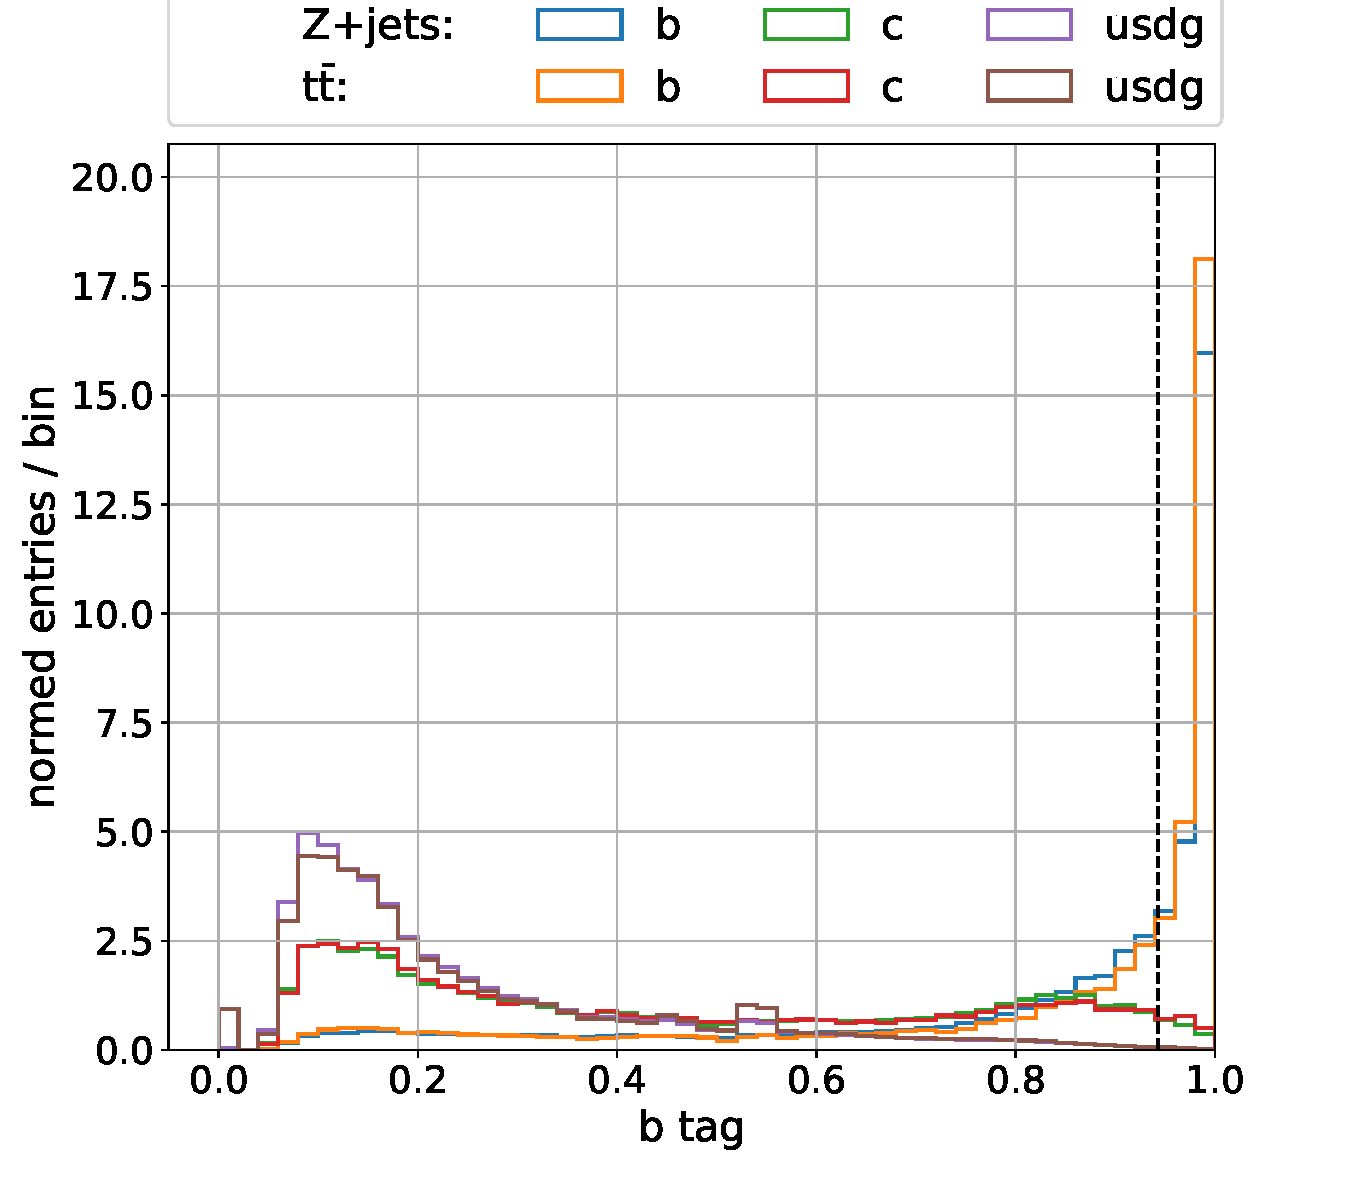
\includegraphics[width=0.45\textwidth]{chapters/Appendix/sectionBtag/figures/bmva_mc.pdf}
    \caption{Distribution of ``bmva" b tagging discriminator for the
    three flavor categories under consideration for Z + jet and
    \ttbar events (left).      
    \label{fig:btag_bmva}}
\end{figure}

\begin{figure}[h!]
    \centering
    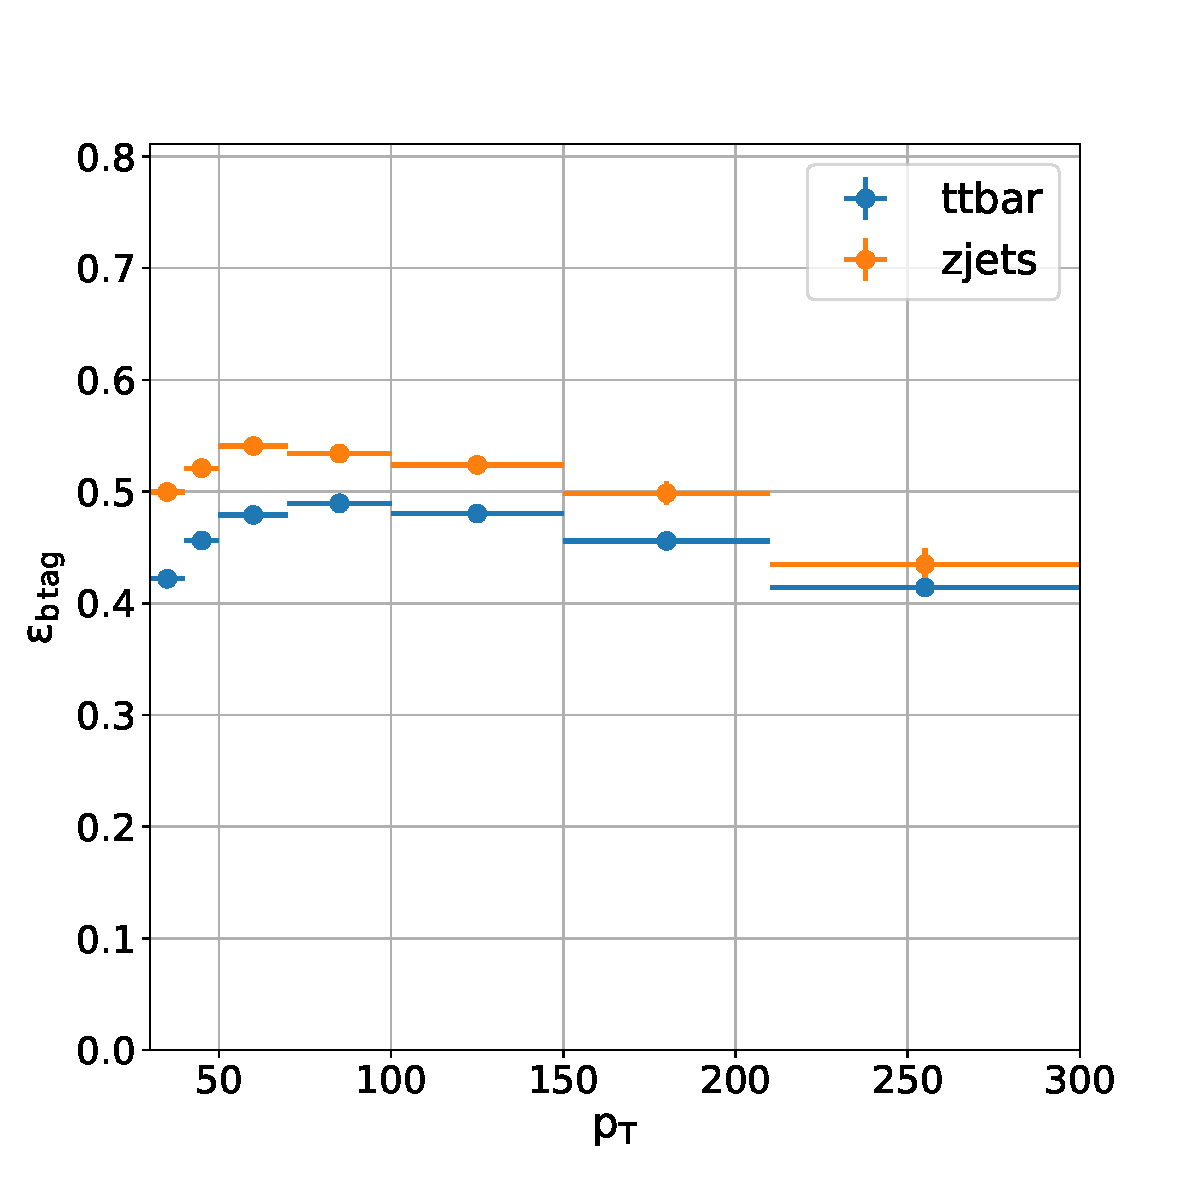
\includegraphics[width=0.3\textwidth]{chapters/Appendix/sectionBtag/figures/bmva_mceff_vs_pt_b}
    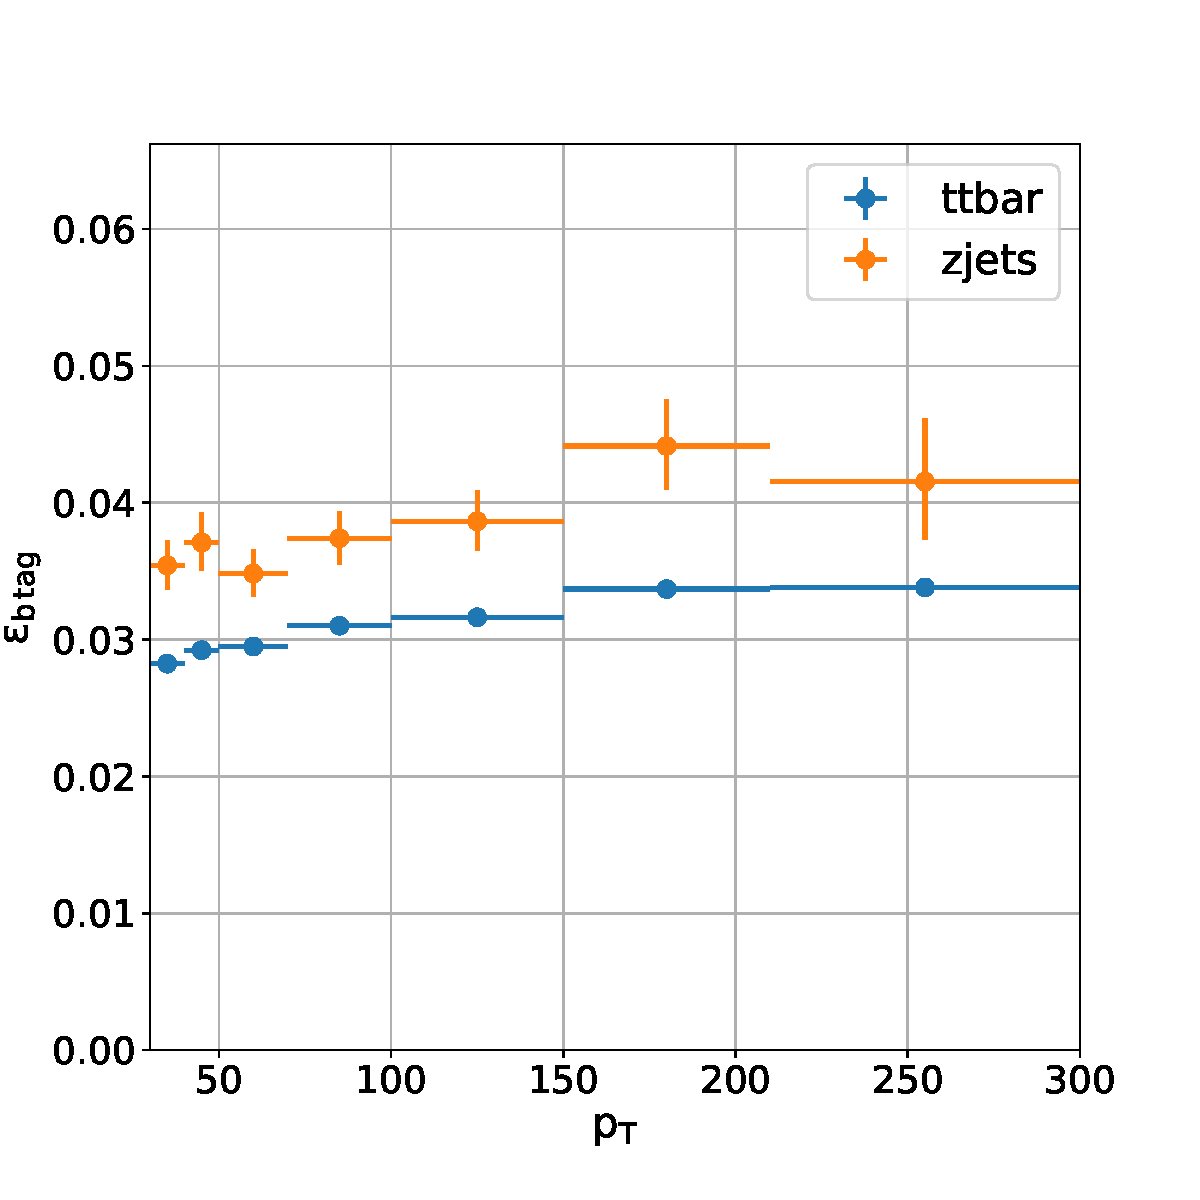
\includegraphics[width=0.3\textwidth]{chapters/Appendix/sectionBtag/figures/bmva_mceff_vs_pt_c}
    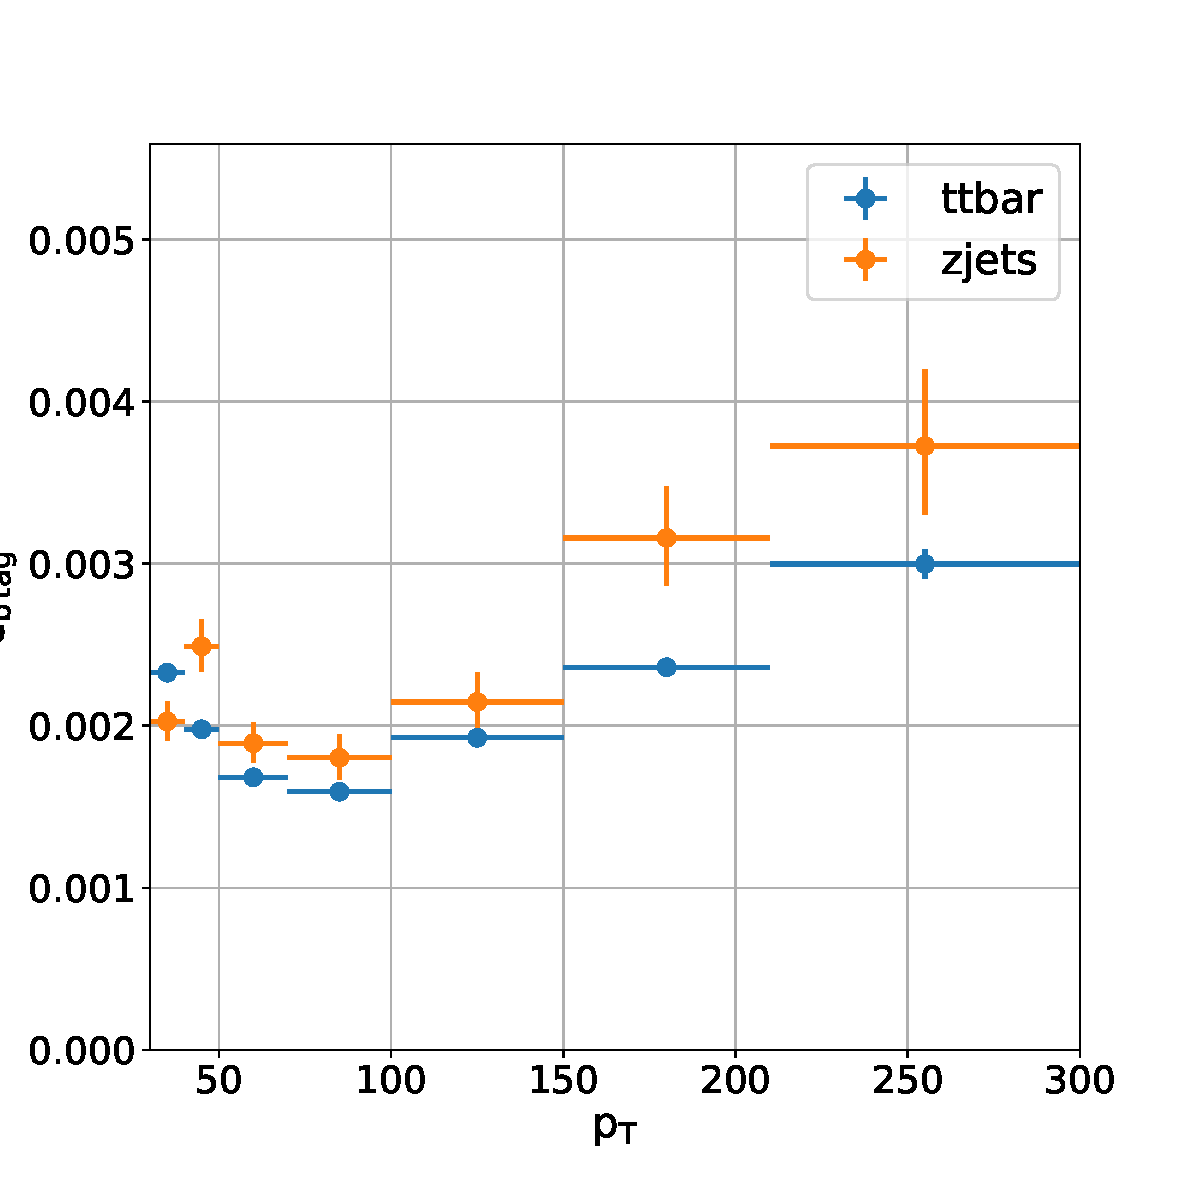
\includegraphics[width=0.3\textwidth]{chapters/Appendix/sectionBtag/figures/bmva_mceff_vs_pt_usdg}
    \caption{Efficiency to b tag a jet originating from a b quark (left), c quark (middle), and light quark (right).
    \label{fig:btag_eff}
    }
\end{figure}

\FloatBarrier



\section{Measurement of Scale Factors for the Single Electron Trigger}
\label{sec:app:eTriggerEff}

\subsection{Measurement Approach}

The data for the measurement of \PW branching fraction is triggered with single electron and single muon trigger. The difference between the trigger efficiencies in the simulation and data is accounted for by applying scale factors to the event weights of simulation. While the scale factors are provided by POG for the correction of single muon trigger efficiencies, those for the single electron has to be measured. 

Single electron trigger, \texttt{HLT\_Ele27\_WPTight\_Gsf}, is used in the $ee$, $e\mu$, $e\tau_h$, $e$+jets channels. Here a customized measurement of scale factor and the associated uncertainties of \texttt{HLT\_Ele27\_WPTight\_Gsf} trigger is performed based on 2016 re-reco dataset with the tag-prob approach. The uncertainty of the scale factor includes both statistical and systematical uncertainty, where systematical uncertainty are estimated by
"two shifts":

\begin{enumerate}
  \item shift up the tagging electron by 10 GeV to simulate a different trigger. This estimates the systematical effect that some L1 seed could have a threshold of 32 GeV.
  \item shift the probing electron pT up and down by 0.5 GeV. This estimates the effect of the electron \pt resolution.
\end{enumerate}


\begin{figure}
    \centering
    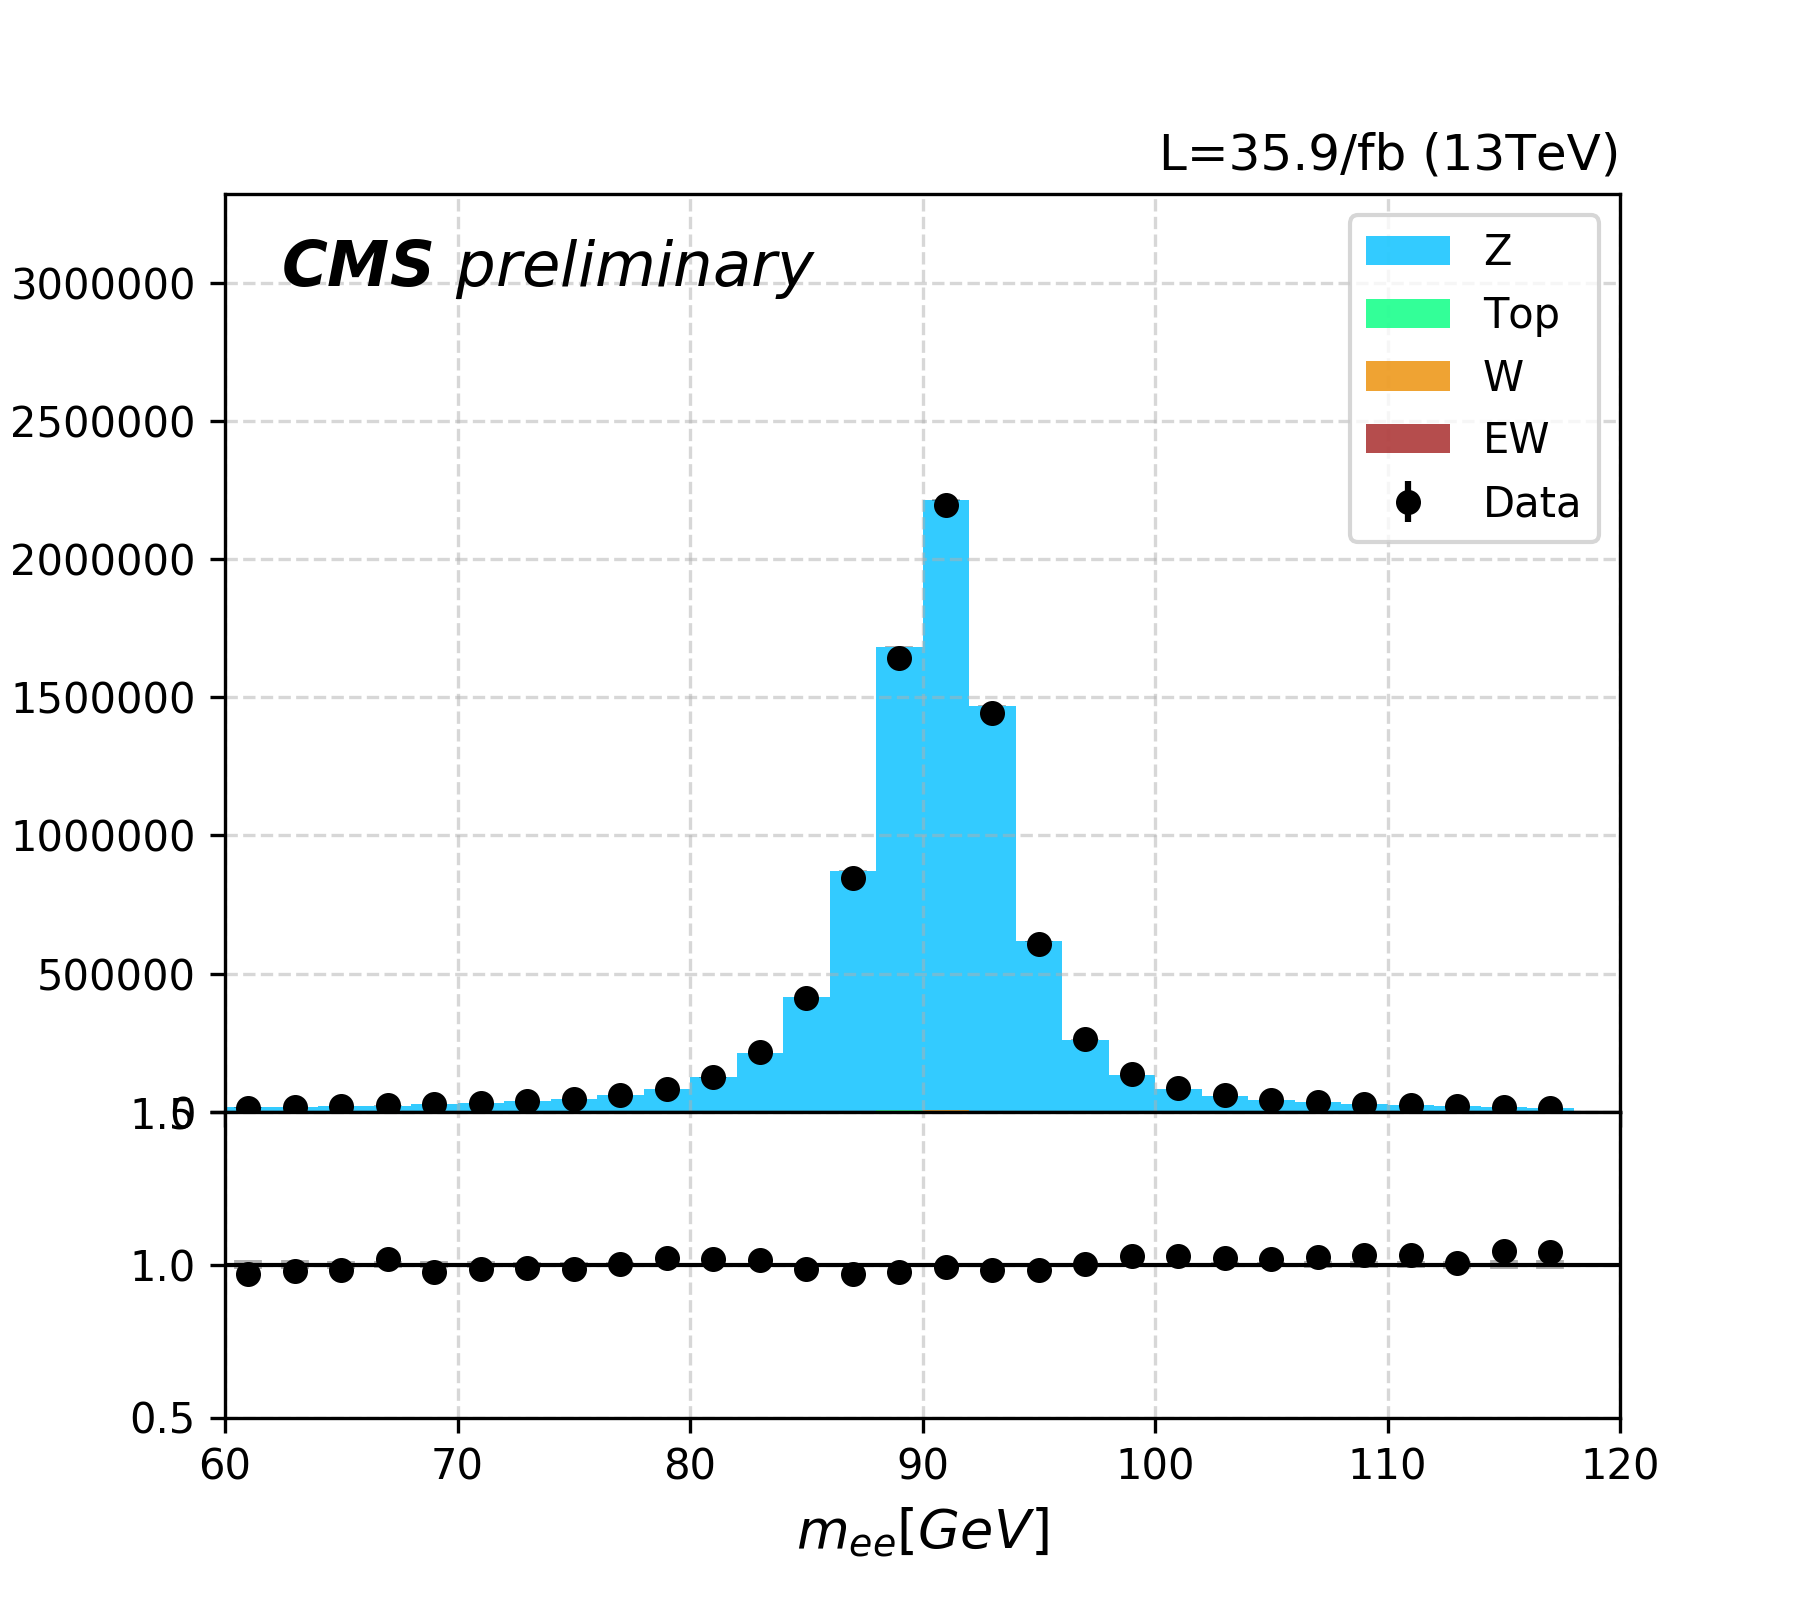
\includegraphics[width=0.6\textwidth]{chapters/Appendix/sectionEleTrigger/figures/dileptonMass_tag30.png}
    \caption{$m_{ee}$ of the selected events for the measurement of the SF of single-electron trigger efficiency.}
    \label{fig:appendix:ele27TriggerSF}
\end{figure}


The dataset used in the measurement is 2016 re-reco \texttt{SingleElectron} dataset with the golden certificate as luminosity mask. The simulations used in the measurement include \texttt{DYJETSToLL\_M-10to50\_amcatnlo}, \texttt{DYJETSToLL\_M-50\_amcatnlo} and \texttt{TT\_powheg}, reweighted to pile-up $\sigma_{mb} = 69.2\pm 2.3$ nb.

% The tag-prob method is used in the measurement of the scale factor of the trigger efficiency.
The electrons are selected with tight identification and tight particle-flow isolation with $p^T_e>20$ GeV and $|\eta_e|<2.5$. Corrections to the electrons in the simulation includes energy scale-smear, reconstruction and isolation. Among selected electrons, tagged electrons are defined as $p^T_e>30$ GeV and outside gap between barrel and endcap calorimeter $1.444<|\eta_e|<1.56$, and match with \texttt{HLT\_Ele27\_WPTight\_Gsf} triggering objects. Events are selected by requiring exactly 2 opposite electrons with at least 1 tagged electron and $60<m_{ee}<120$ GeV. This event selection yields a sample of events significantly dominated by Drell-Yan process. The distribution of $m_{ee}$ is shown in fig~\ref{fig:appendix:ele27TriggerSF}. The purity of Drell-Yan (DY) are very high in the selected events. Thus a signal-backgound fit is not necessary to get DY yields.





In each event, if one electron is tagged, the other become a prob. Each event provides either one or two tag-prob pairs. A prob is passing if it match with \texttt{HLT\_Ele27\_WPTight\_Gsf} triggering objects. The trigger efficiencies are calculated by the ratio between the number of passing probs over the total probs in $\pt-\eta$ bins, 

\begin{equation}
    \epsilon (\pt, \eta) = \frac{ N_{\rm passing} (\pt, \eta) } {  N_{\rm total} (\pt, \eta) }.
\end{equation}

\noindent The scale factors are derived by taking the ratio between efficiencies in the data over MC,
\begin{equation}
SF (\pt, \eta) = \frac{\epsilon_{\rm{data}} (\pt, \eta) }{\epsilon_{\rm{MC}} (\pt, \eta) }.
\end{equation}



\subsection{Result of the Scale Factors}

In 2016 B-F, the data efficiency in the endcap decreases because there is a decrease of signal over noise ratio associated 
to loss of	tracking hits caused by problems in the pre-amplifier of the APV chip. 
In the mid August 2016, this problem of Si-strip in endcap region is fixed by increase the drain speed of the pre-amplifier. Thus the 
trigger efficiencies are improved in 2016 GH. So the measurement of the scale factor of the trigger efficiency is divided into to
two parts based on data taking periods, the 2016 B-F and 2016 GH.

The 2D maps of $\epsilon_{\rm{data}}$, $\epsilon_{\rm{MC}}$ and $SF$ in both 2016 B-F and 2016 GH are shown in Figure~\ref{fig:appendix:ele27SF}. Figure~\ref{fig:appendix:ele27SFperiods} 
shows the $SF$ in each 2016 data taking period, where the improvement in the G period is clear.



\begin{figure}
    \centering
    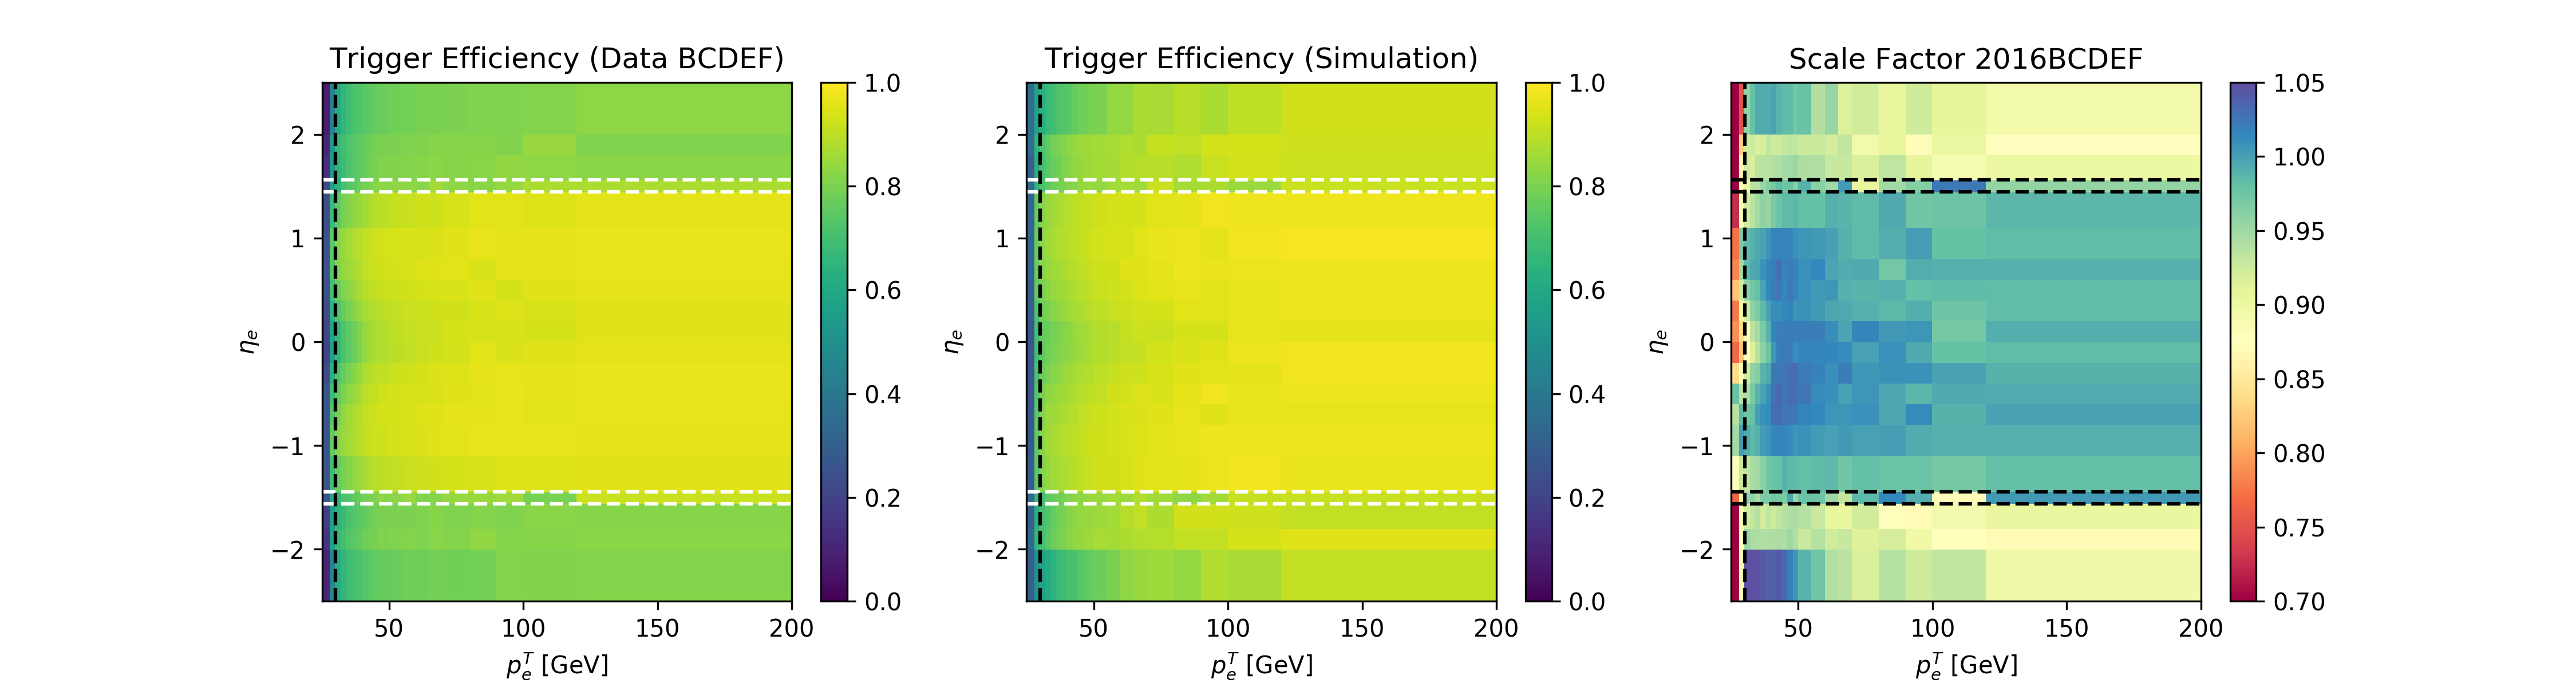
\includegraphics[width=0.99\textwidth]{chapters/Appendix/sectionEleTrigger/figures/eff2d_BCDEF.png}
    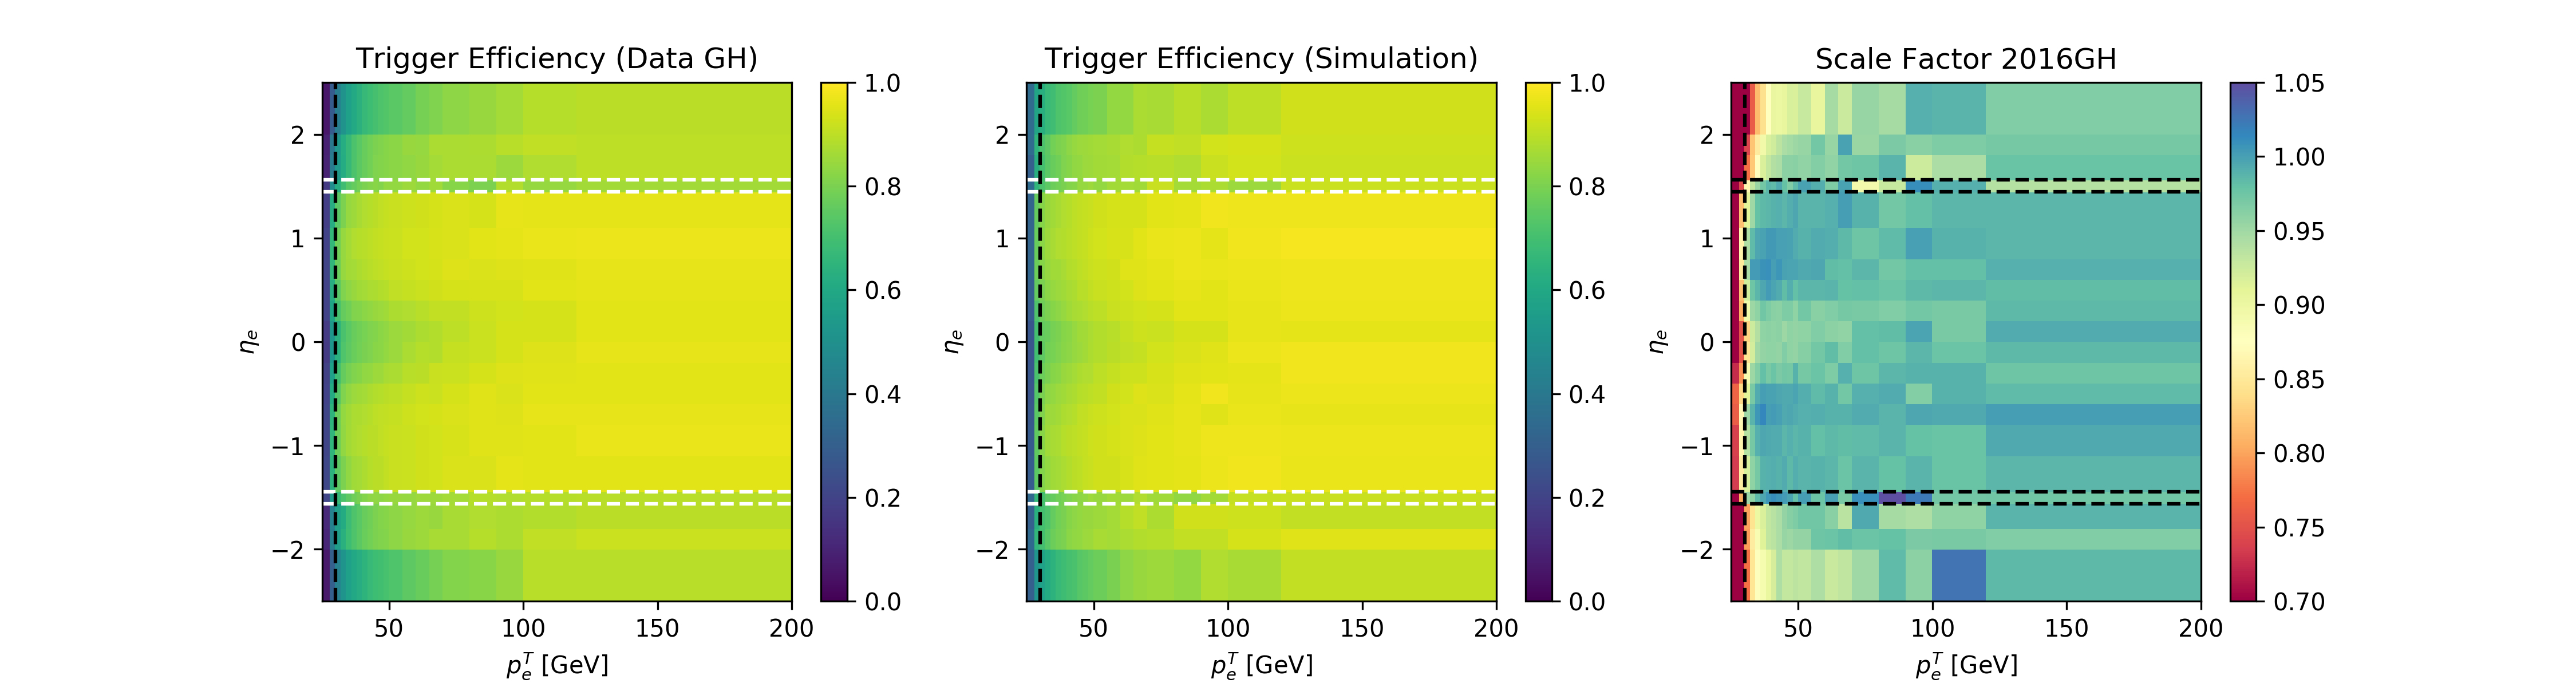
\includegraphics[width=0.99\textwidth]{chapters/Appendix/sectionEleTrigger/figures/eff2d_GH.png}
    \caption{The 2D maps of $\epsilon_{\rm{data}}$, $\epsilon_{\rm{MC}}$ and $SF$ in both 2016 B-F and 2016 GH.}
    \label{fig:appendix:ele27SF}
\end{figure}



\begin{figure}
    \centering
    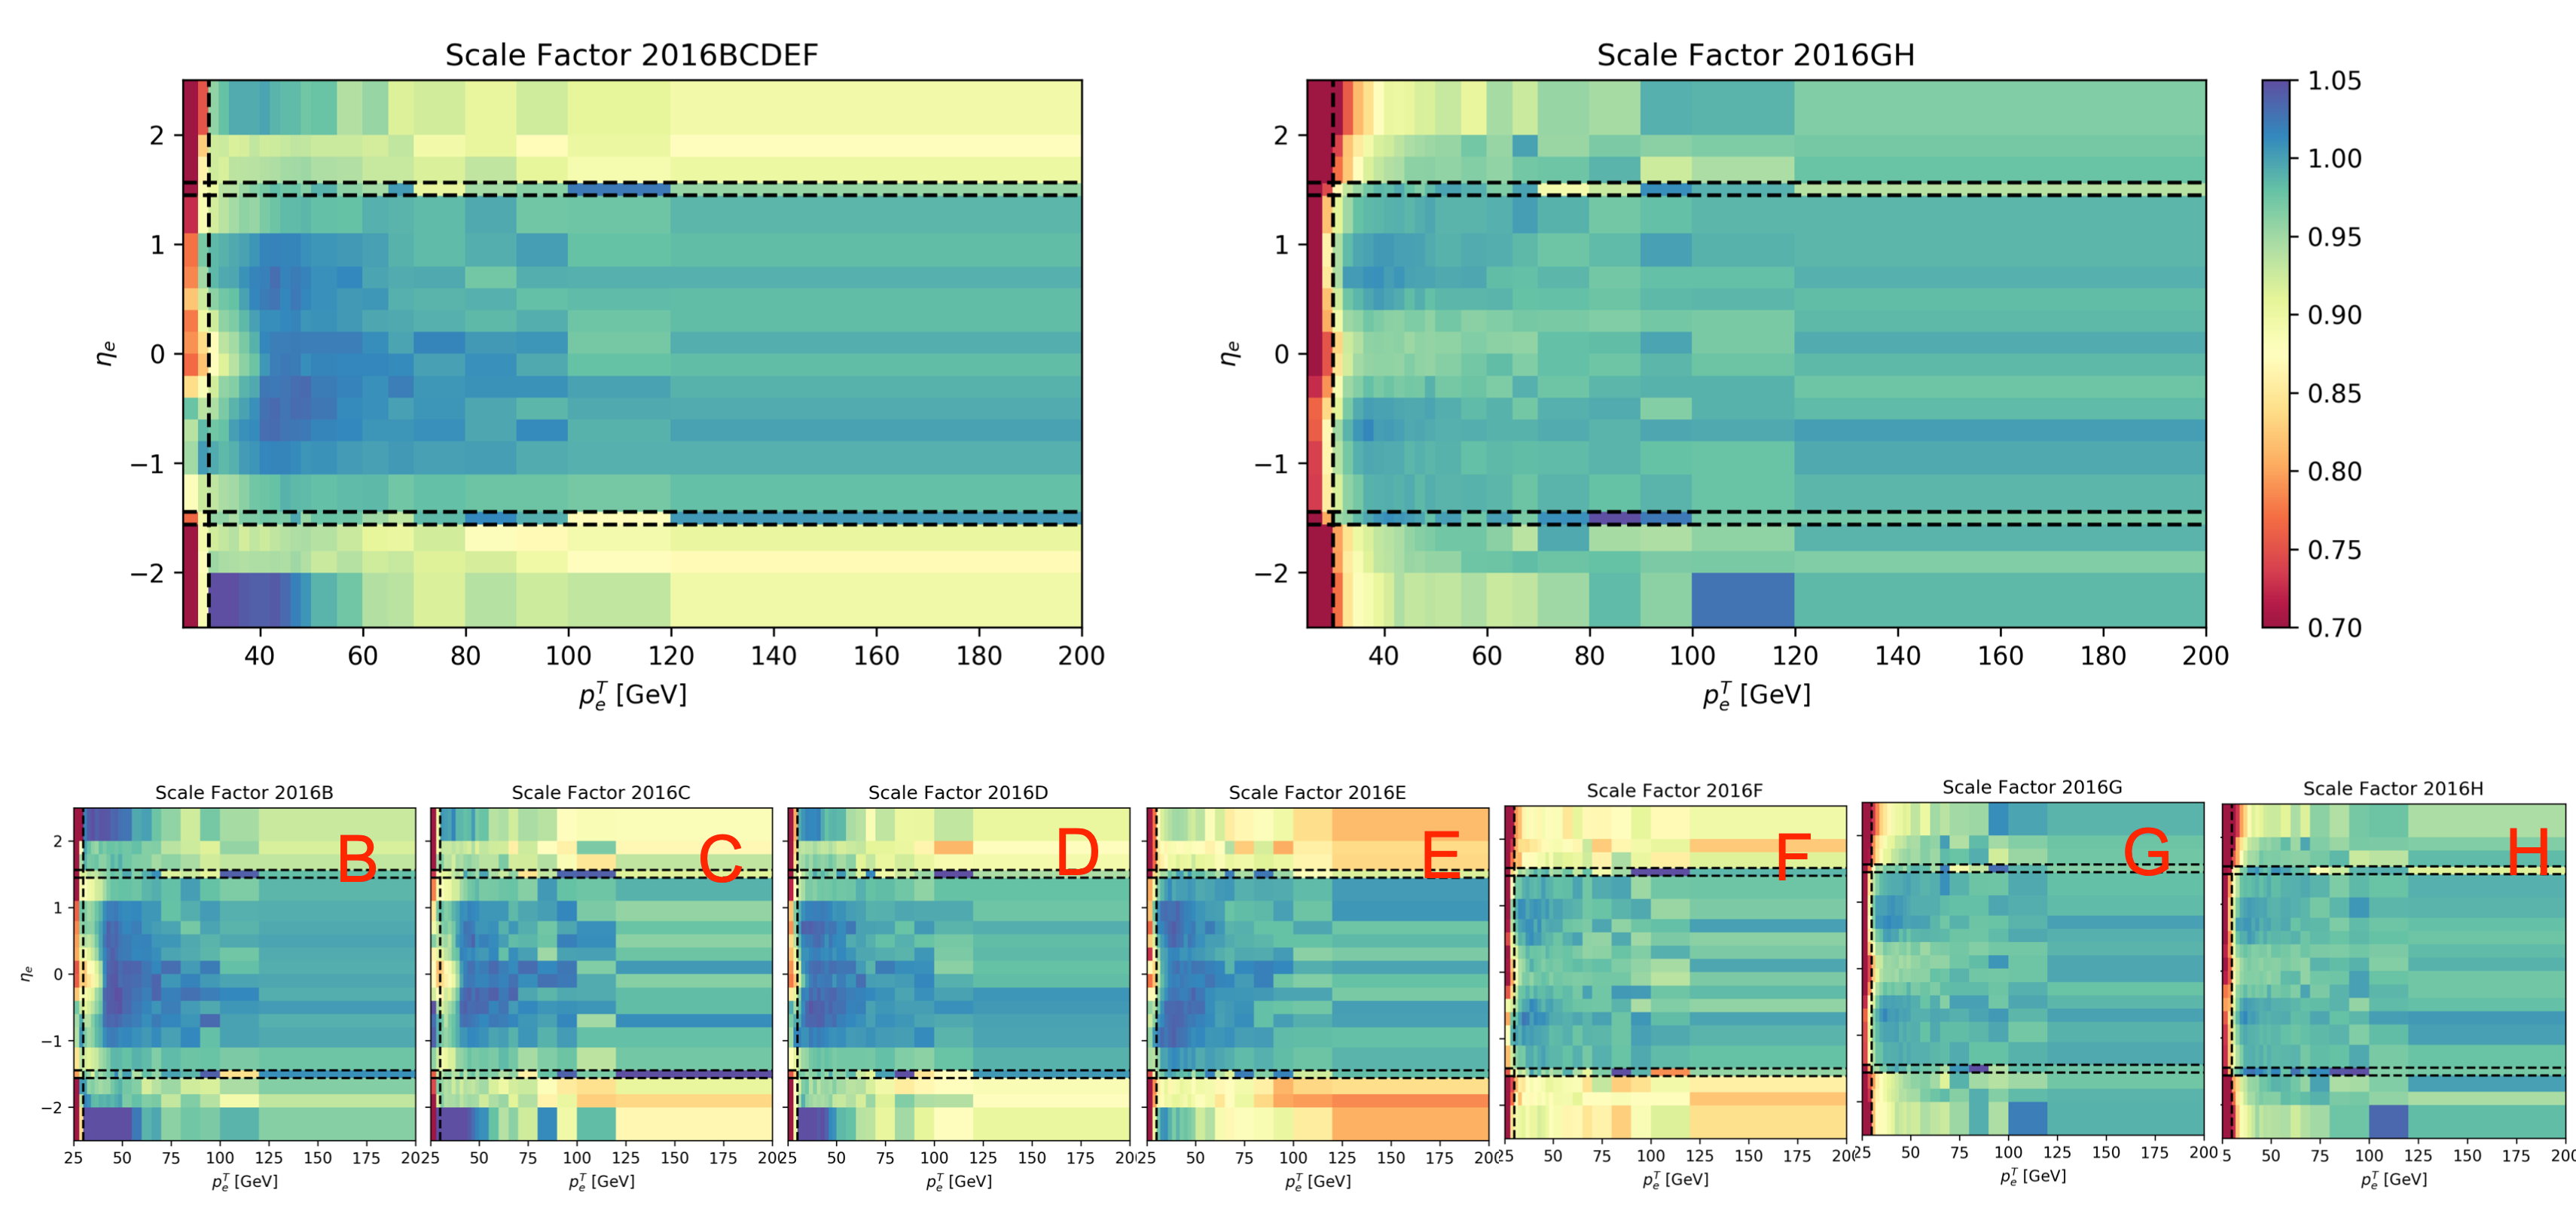
\includegraphics[width=0.99\textwidth, trim=0 0 0 1.1\textwidth, clip]{chapters/Appendix/sectionEleTrigger/figures/eTrSF_value.png}
    \caption{$SF$ in each 2016 data taking period.}
    \label{fig:appendix:ele27SFperiods}
\end{figure}





For the two parts, 2016 B-F and GH, the systematical uncertainties are estimated by the "two shifts" approach described above. 
The total uncertainty combines the statistical and systematical uncertainties from tag and prob "two shifts".
The final result of the SF and the associated uncertainties are shown in fig~\ref{fig:eTrSF_err_BCDEF} and \ref{fig:eTrSF_err_GH}.

\begin{figure}
    \centering
    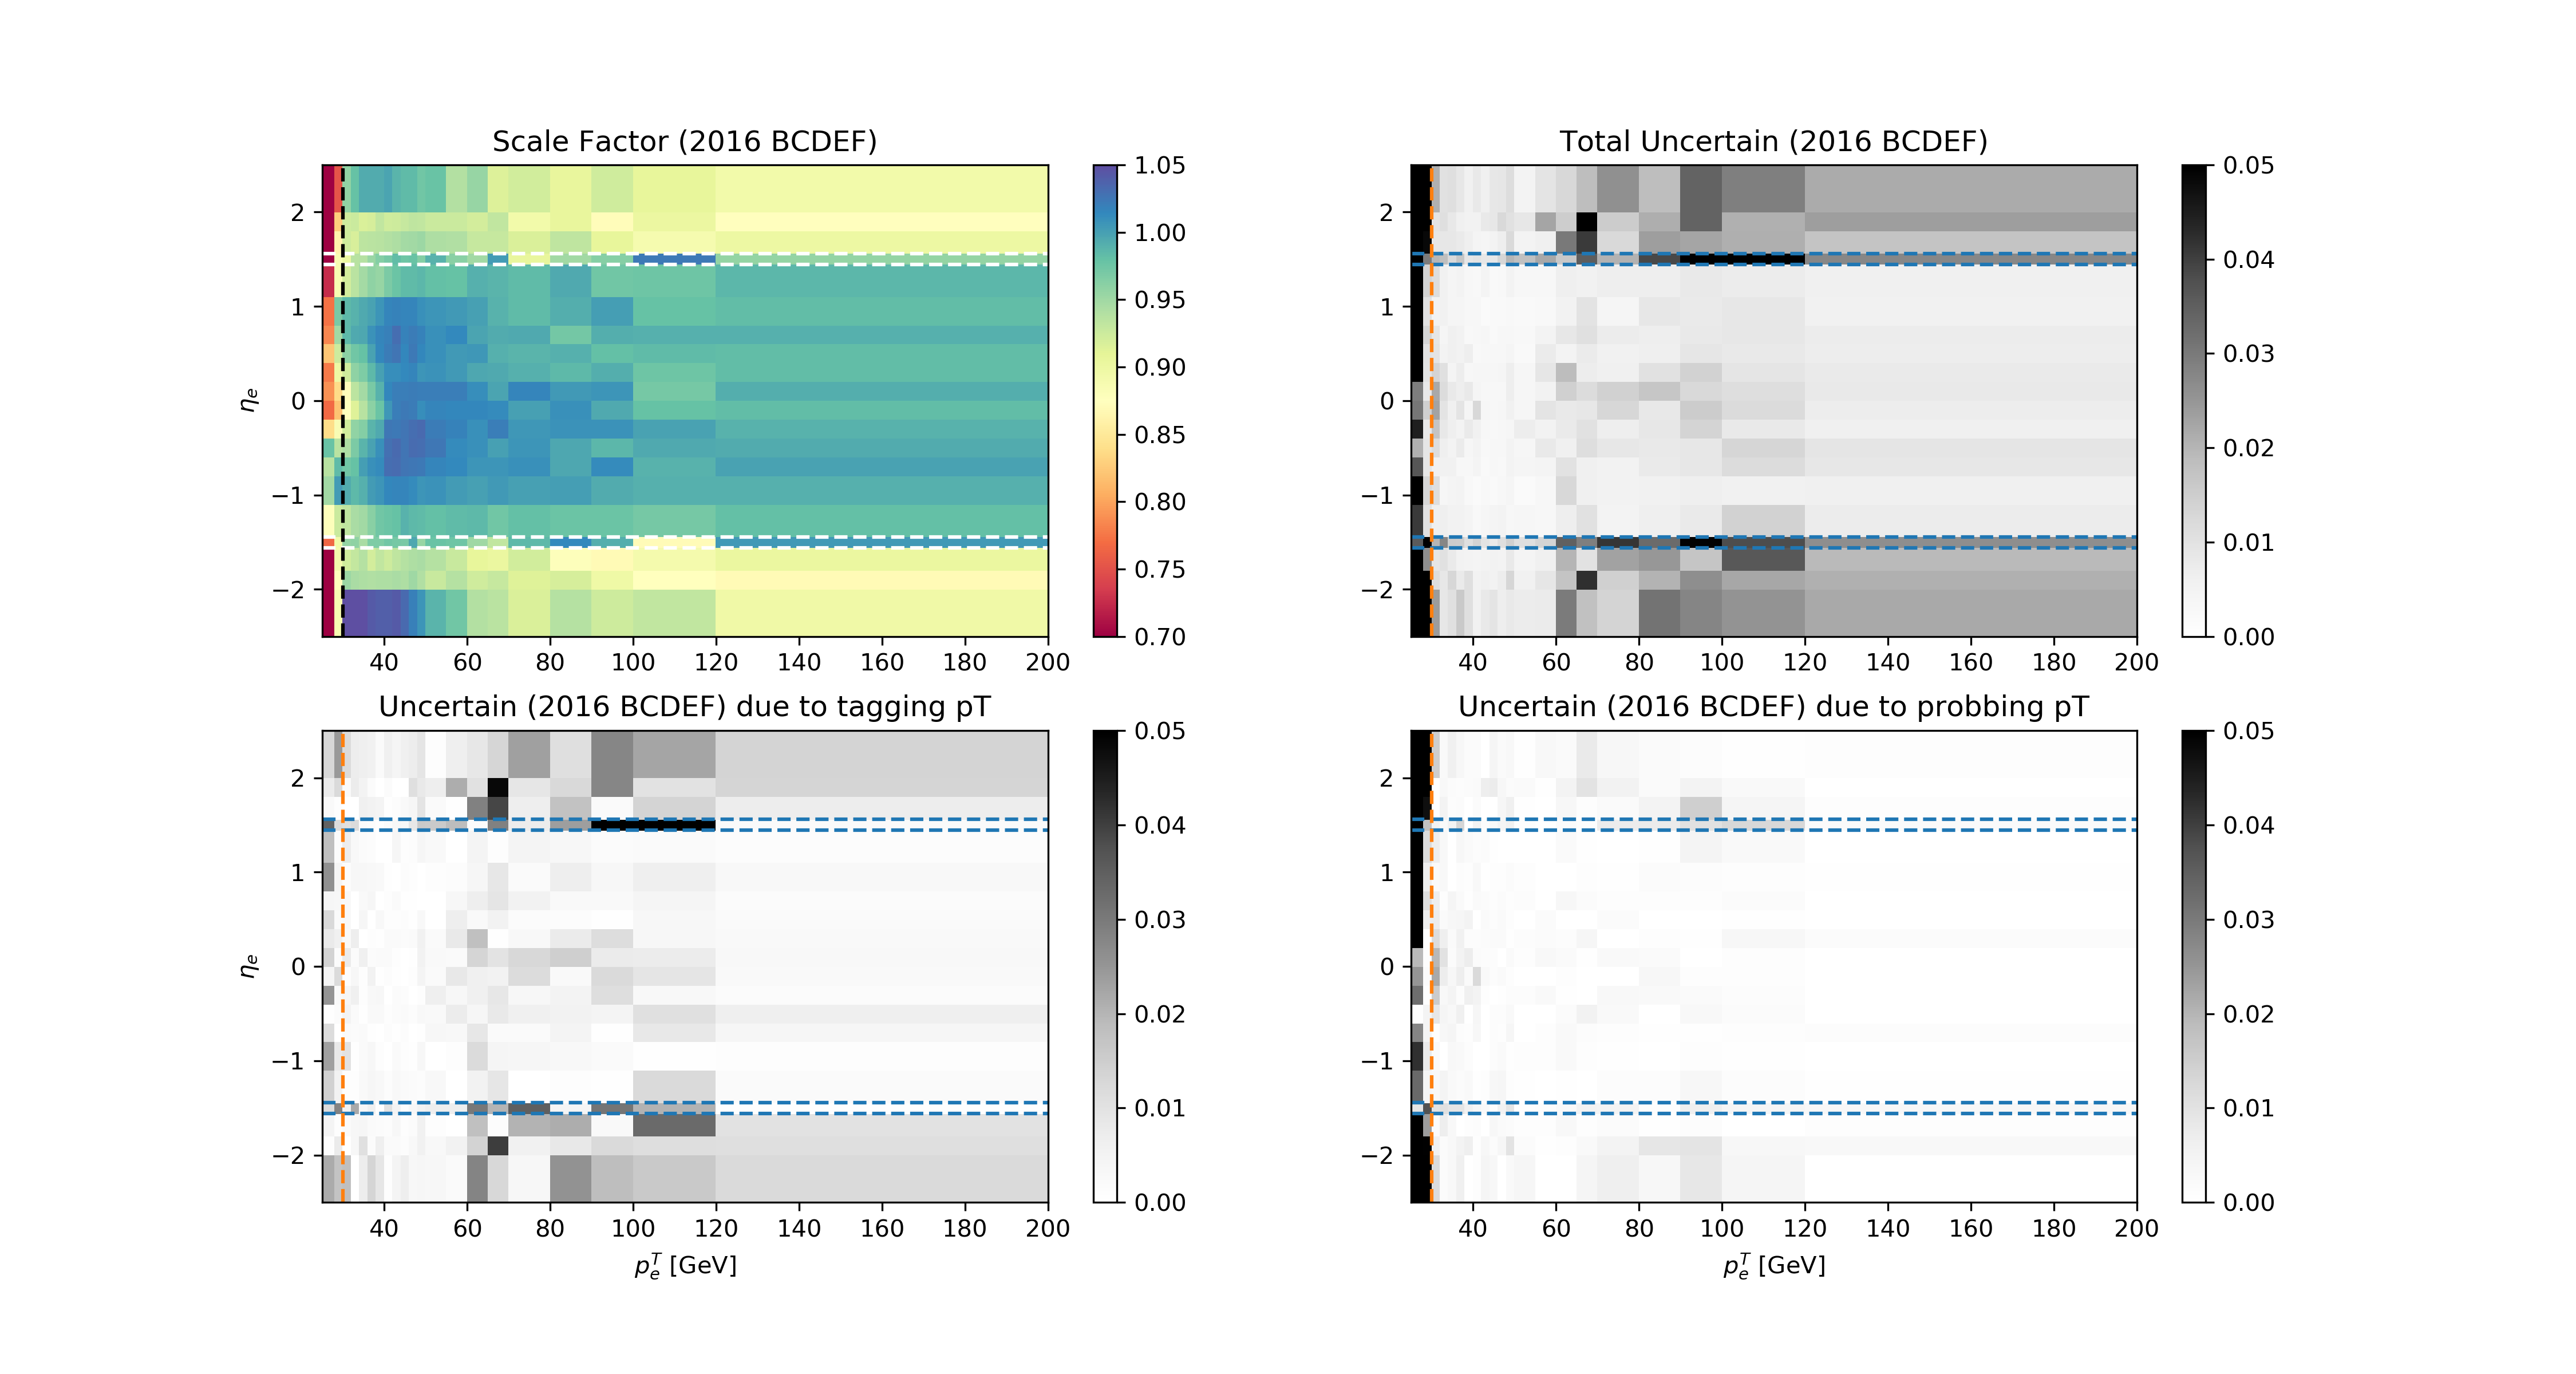
\includegraphics[width=0.99\textwidth]{chapters/Appendix/sectionEleTrigger/figures/result_BCDEF.png}
    
    \caption{SF and the associated uncertainties in the 2016 B-F.}
    \label{fig:eTrSF_err_BCDEF}
\end{figure}

\begin{figure}
    \centering
    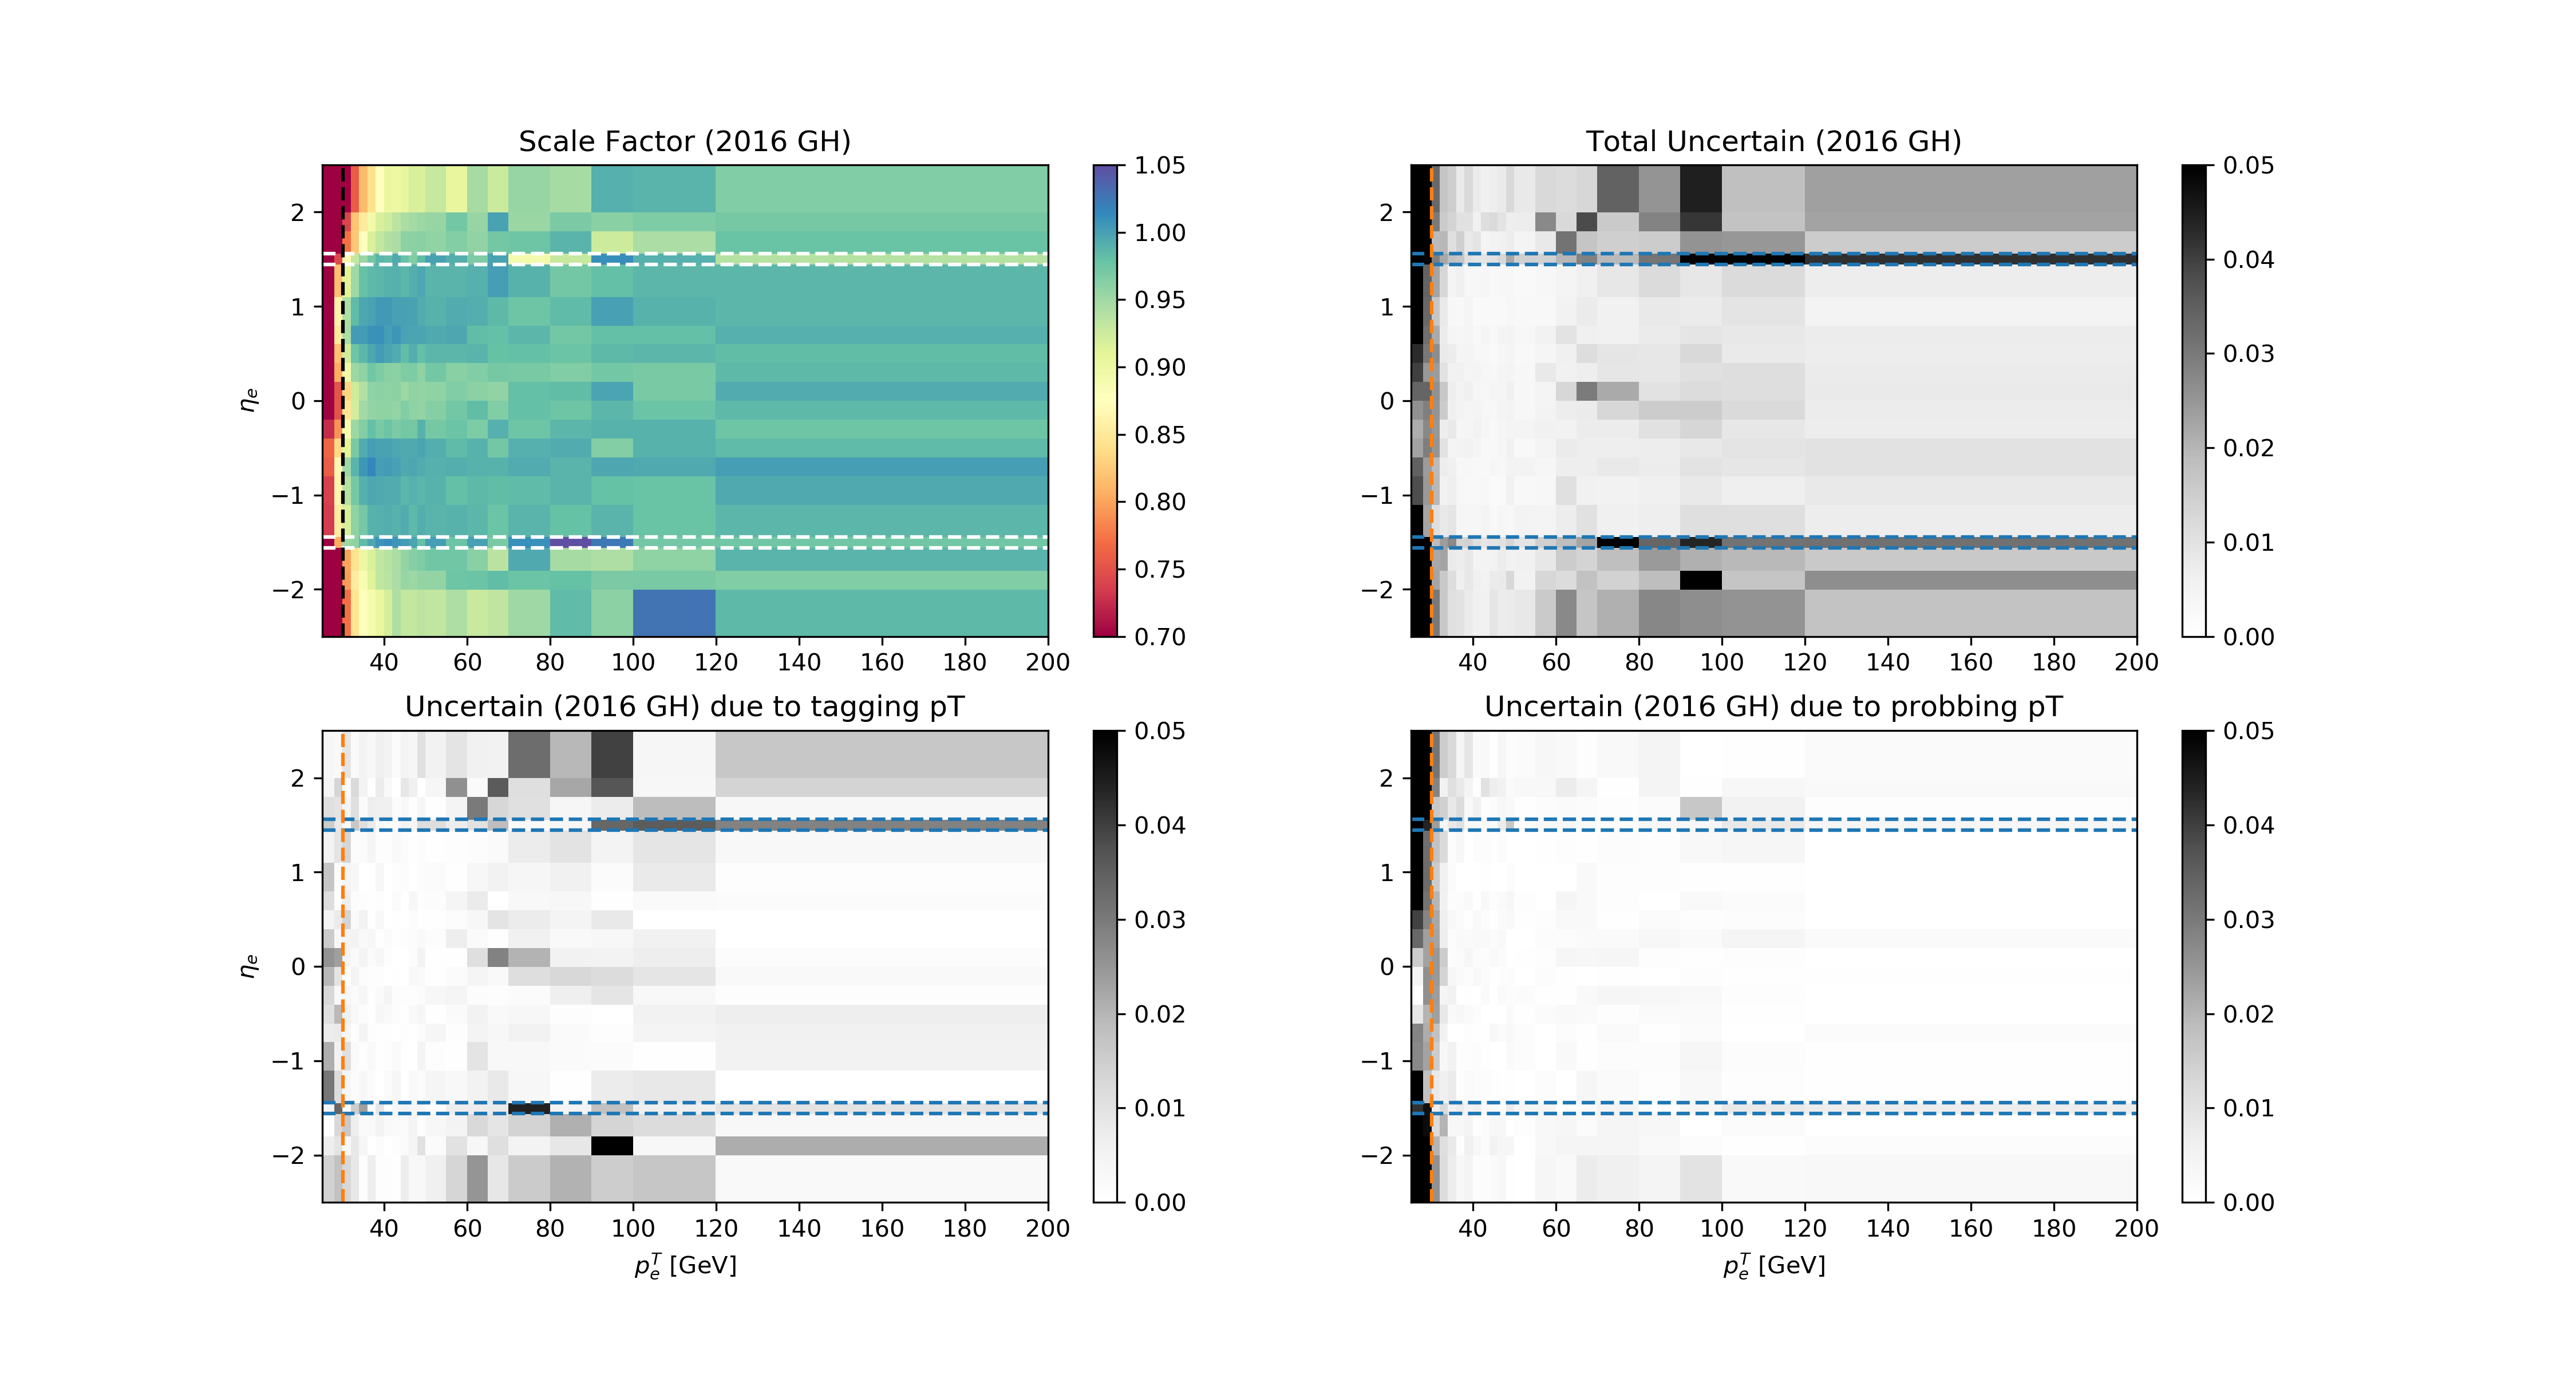
\includegraphics[width=0.99\textwidth]{chapters/Appendix/sectionEleTrigger/figures/result_GH.png}
    
    \caption{SF and the associated uncertainties in the 2016 GH.}
    \label{fig:eTrSF_err_GH}
\end{figure}

\FloatBarrier



\chapter{Measurement of \texorpdfstring{$j \to \tau_h$}{Lg} Scale Factor}

\begin{figure}
    \centering
    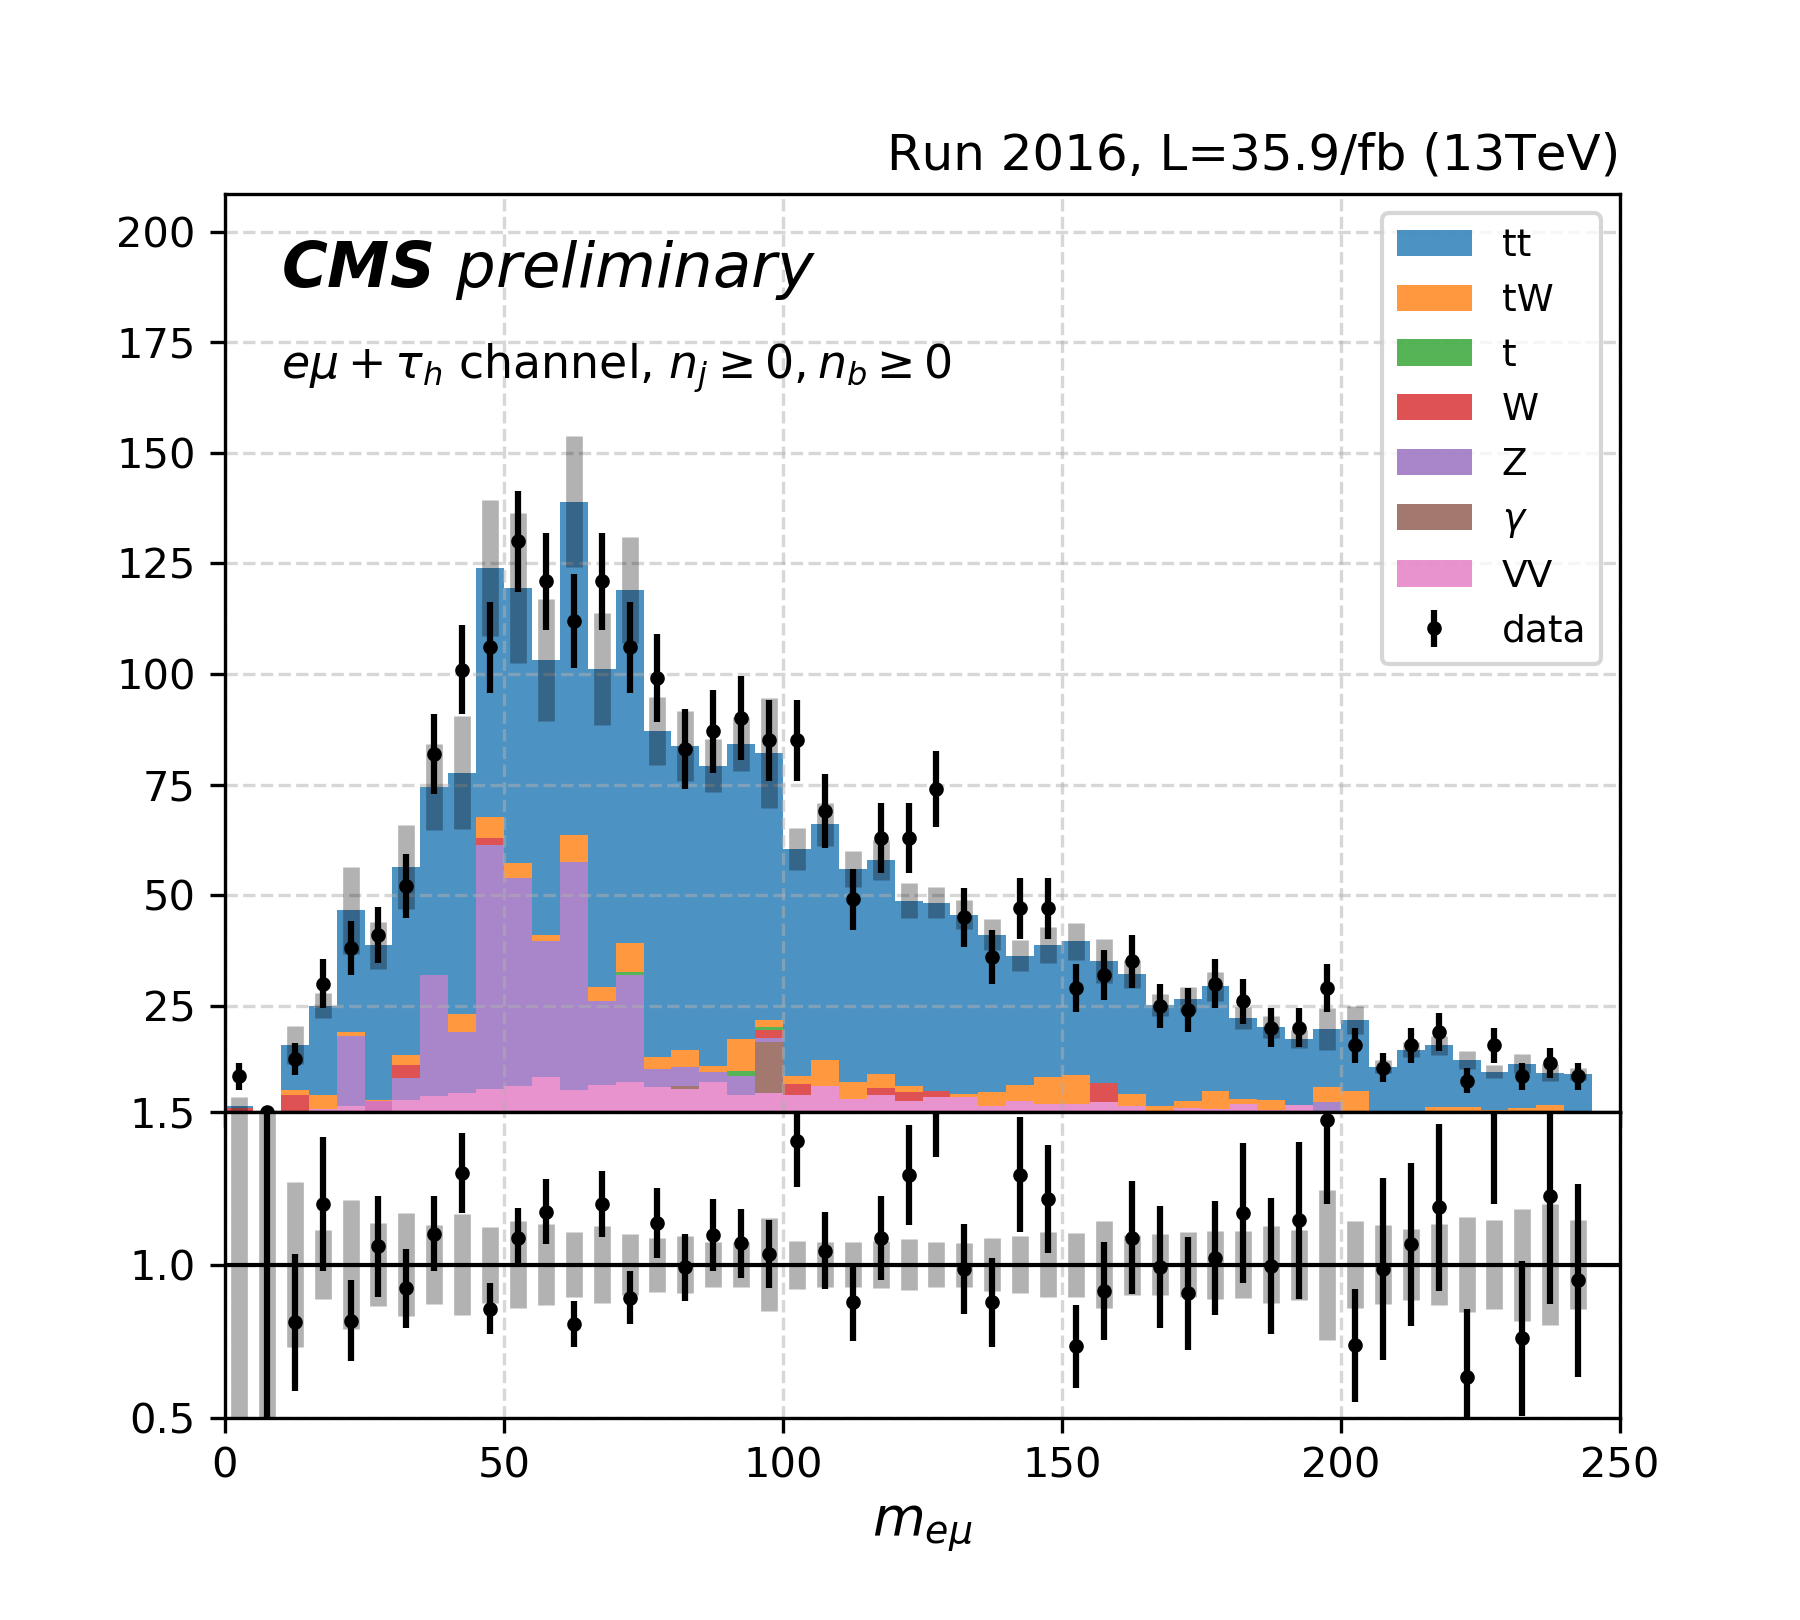
\includegraphics[width=0.4\textwidth]{chapters/Appendix/sectionJetToTauh/figures/emutau_dilepton_mass_pickles_lltauTight.png}
    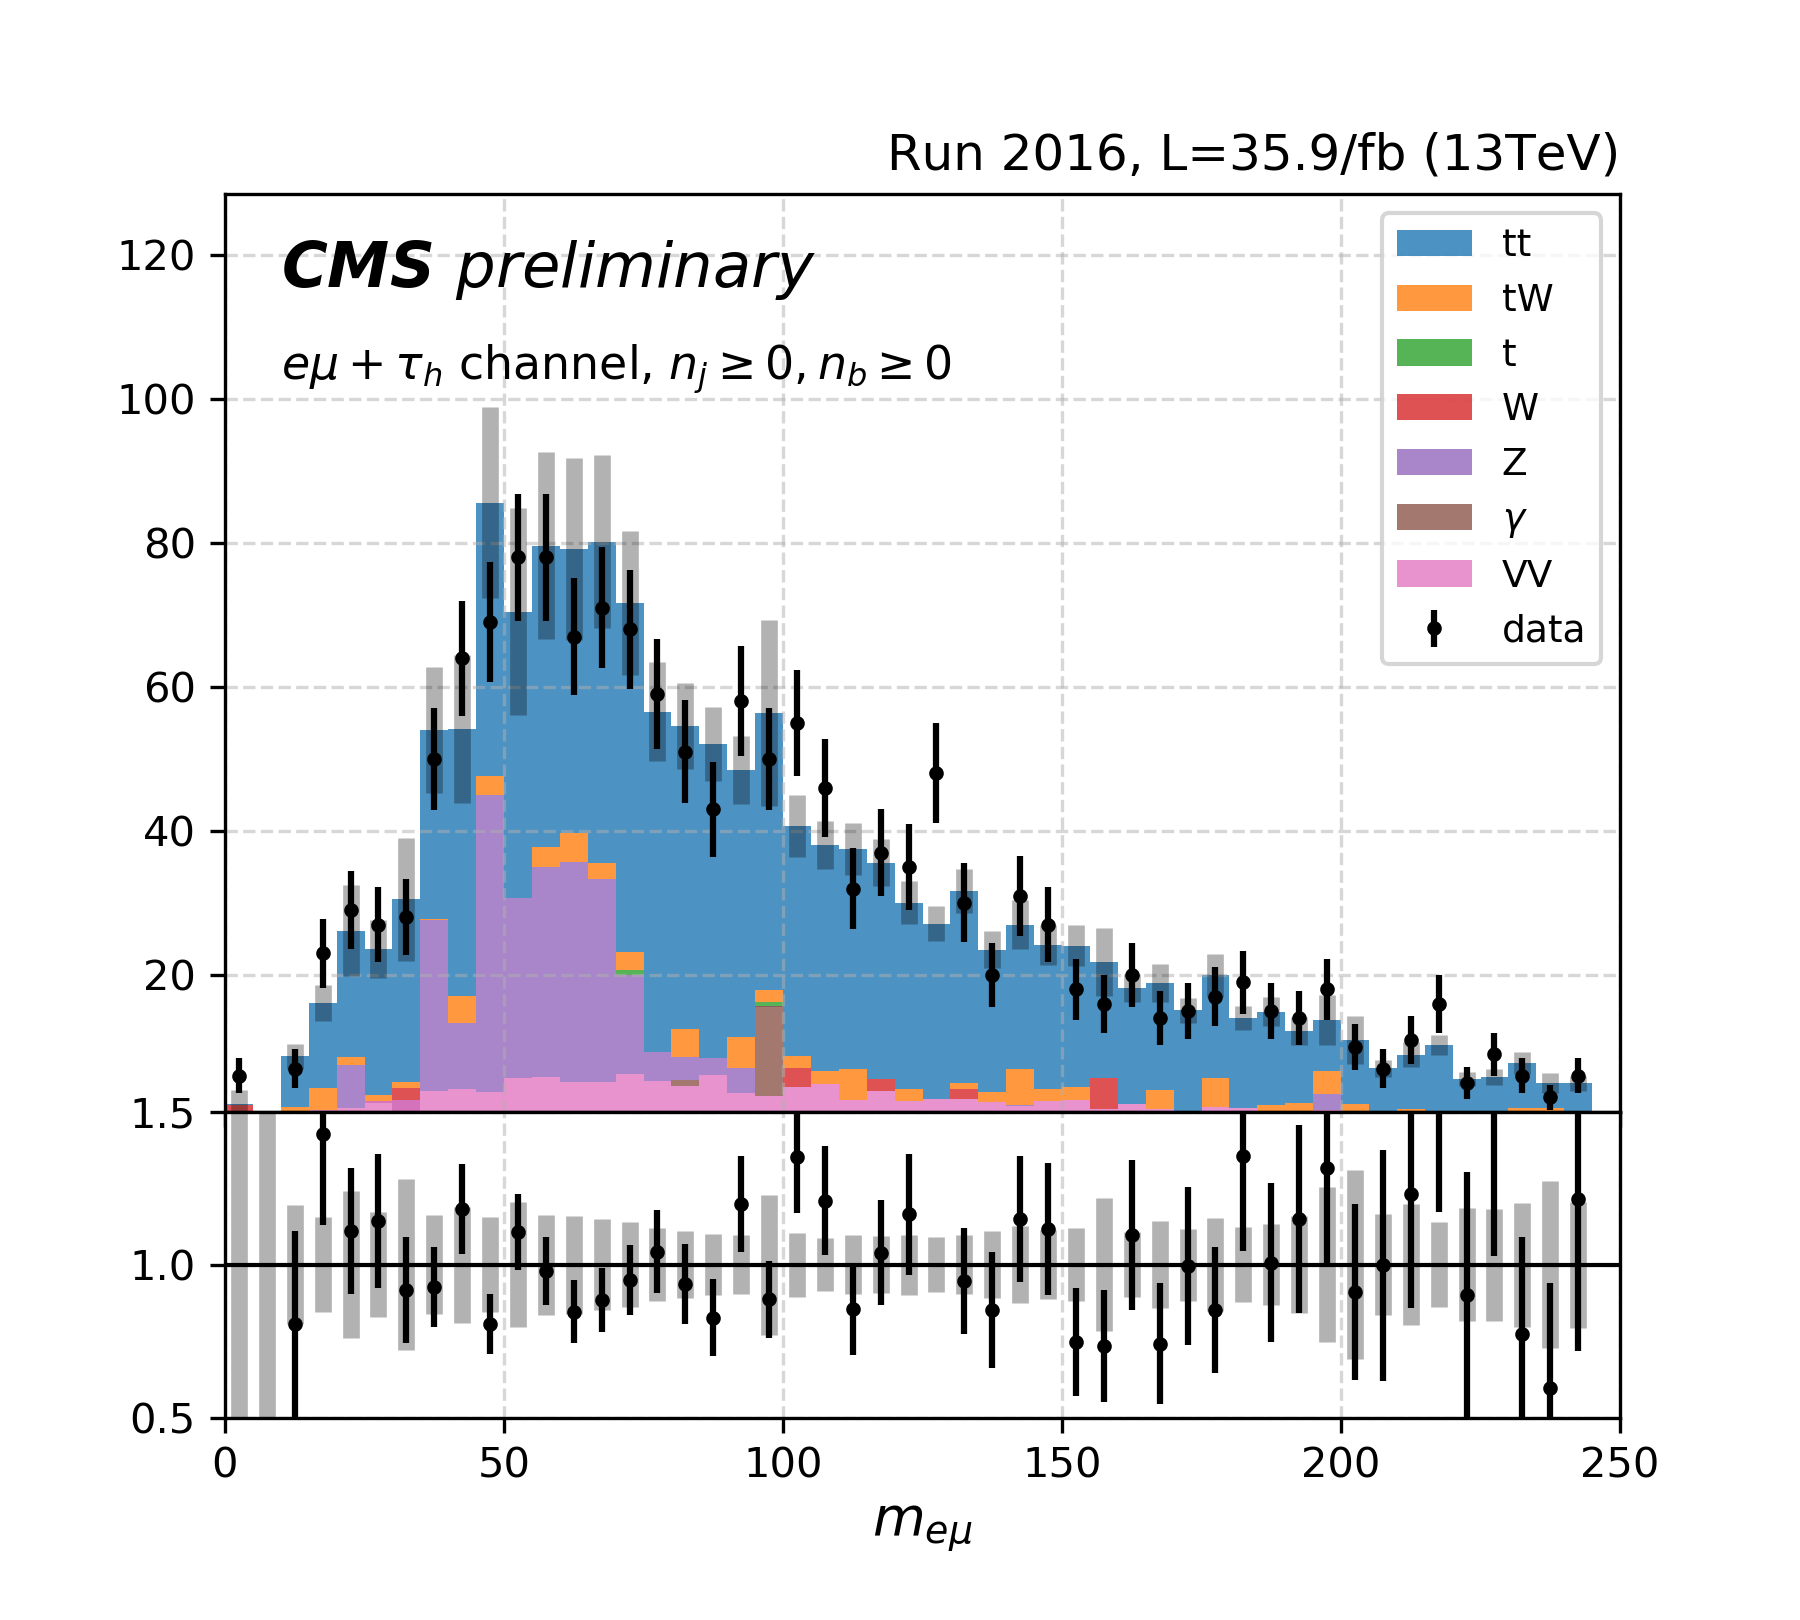
\includegraphics[width=0.4\textwidth]{chapters/Appendix/sectionJetToTauh/figures/emutau_dilepton_mass_pickles_lltauVTight.png}
    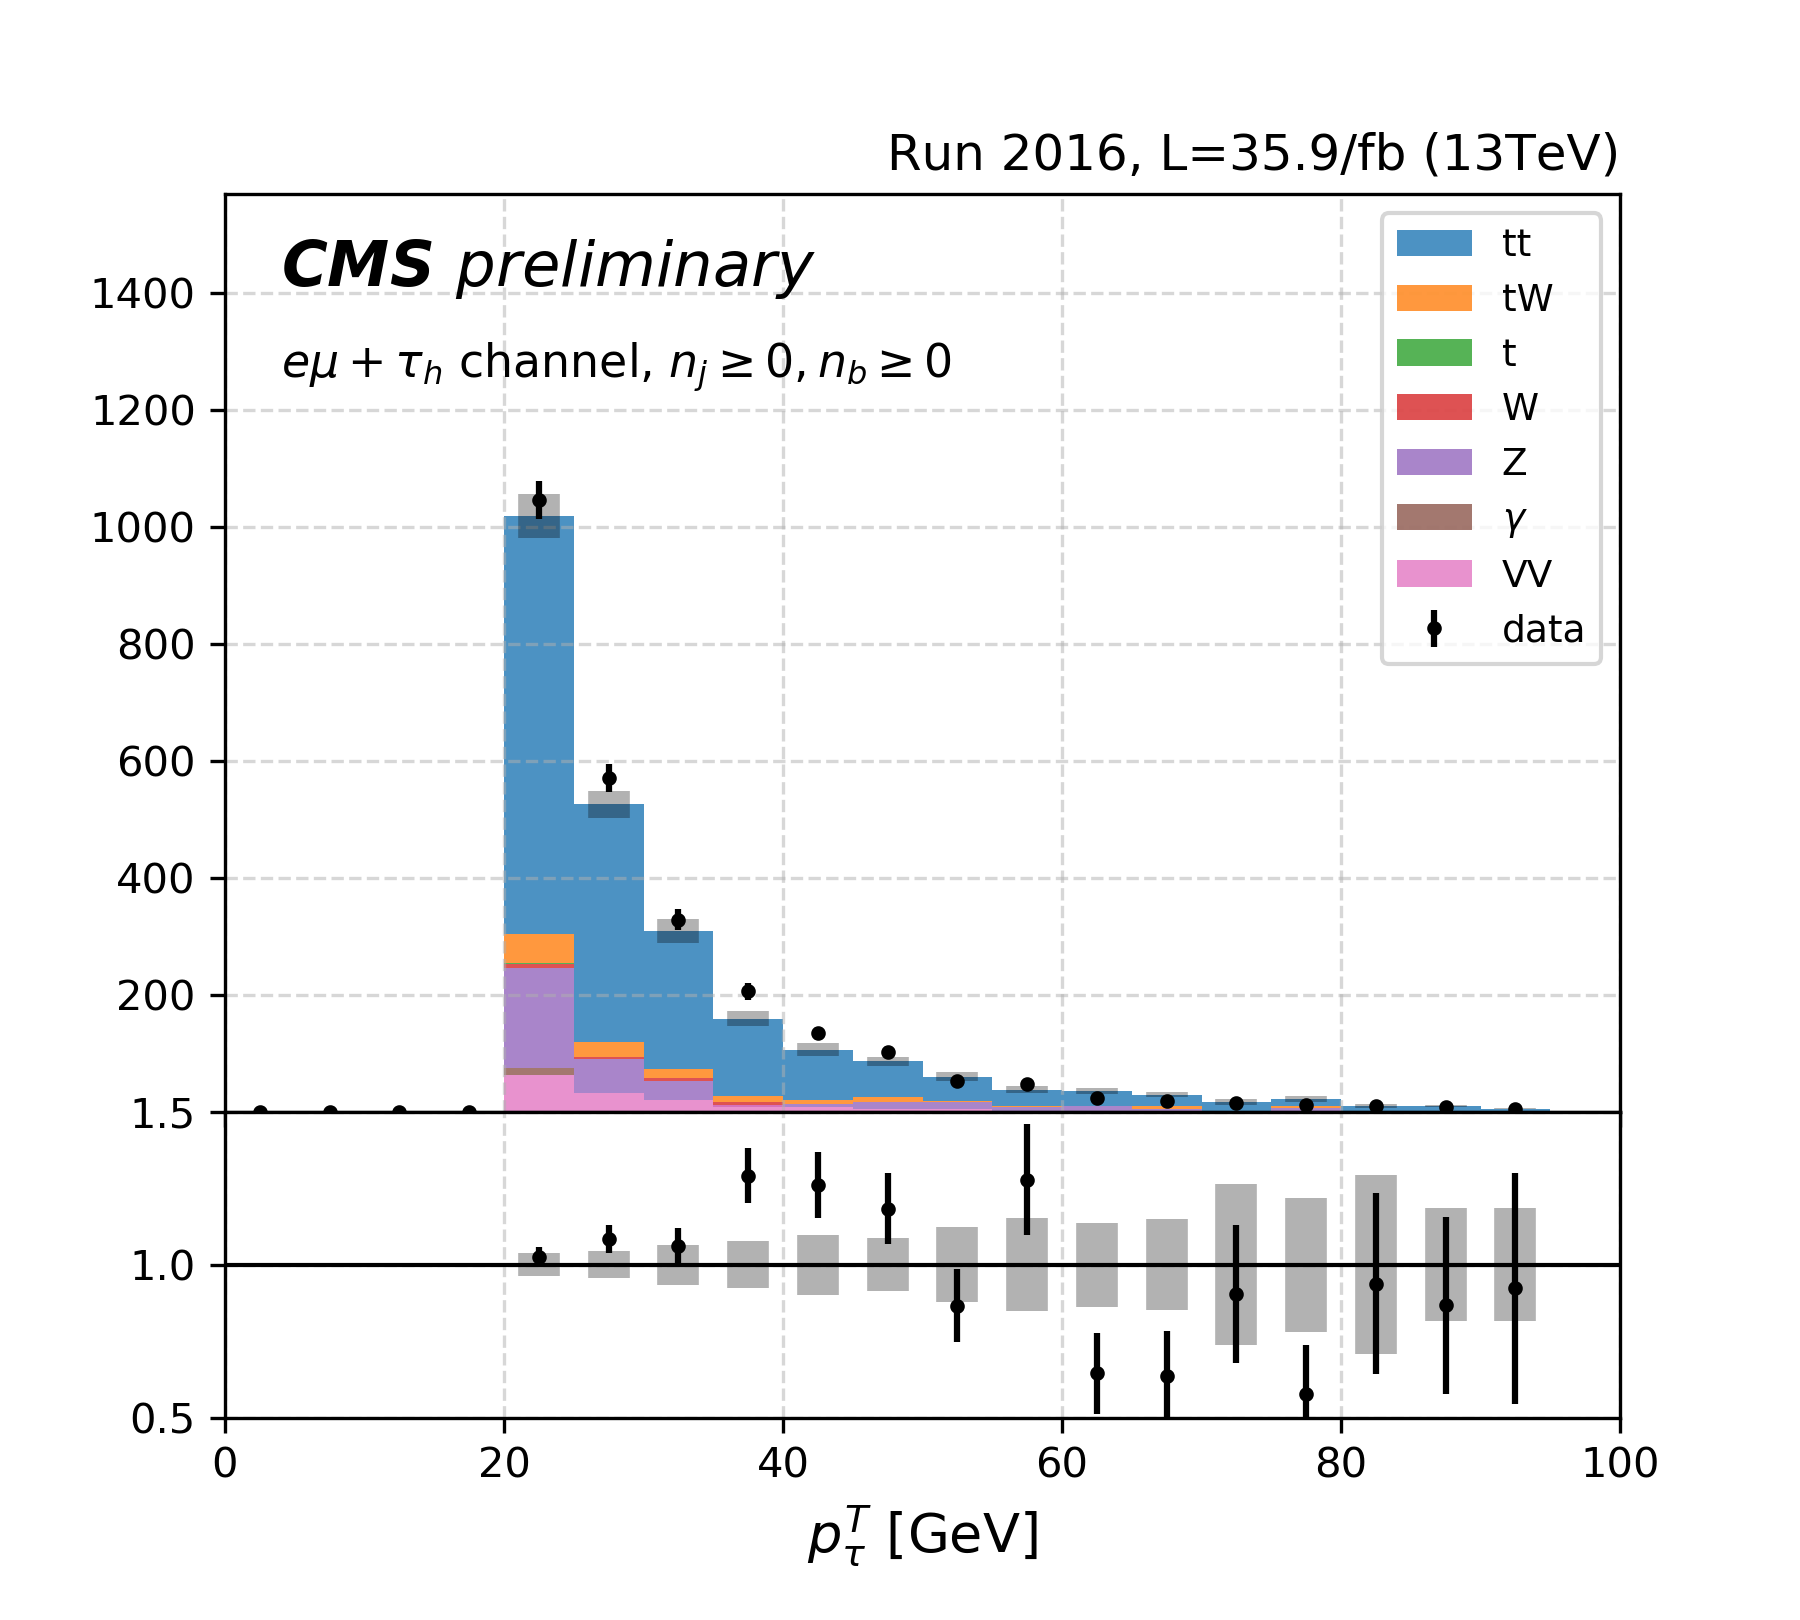
\includegraphics[width=0.4\textwidth]{chapters/Appendix/sectionJetToTauh/figures/emutau_tauPt_pickles_lltauTight.png}
    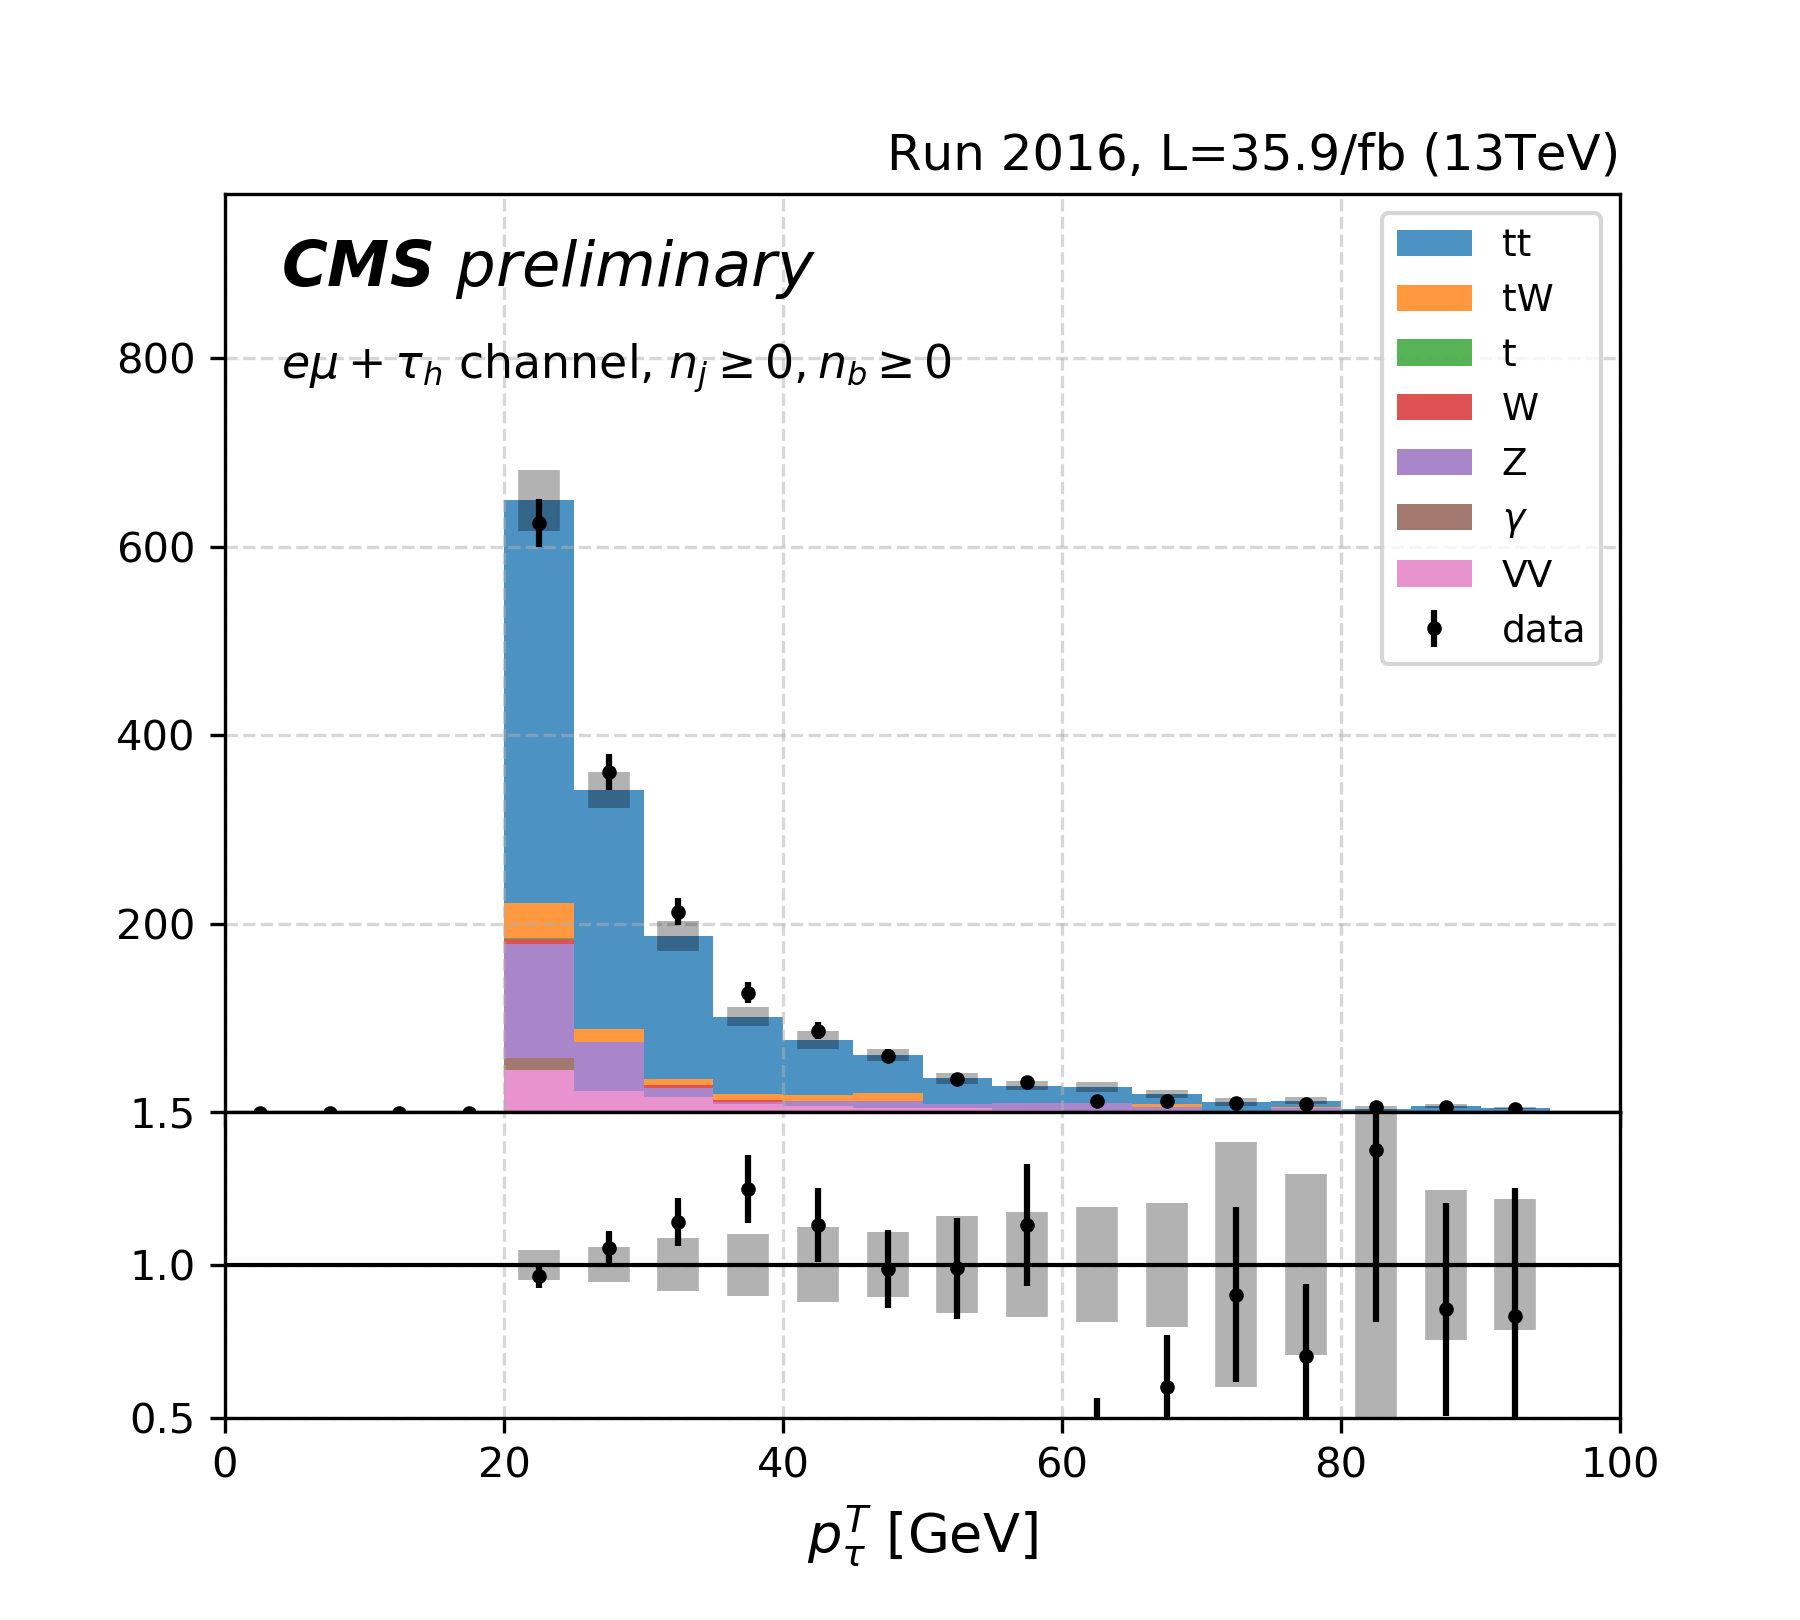
\includegraphics[width=0.4\textwidth]{chapters/Appendix/sectionJetToTauh/figures/emutau_tauPt_pickles_lltauVTight.png}
    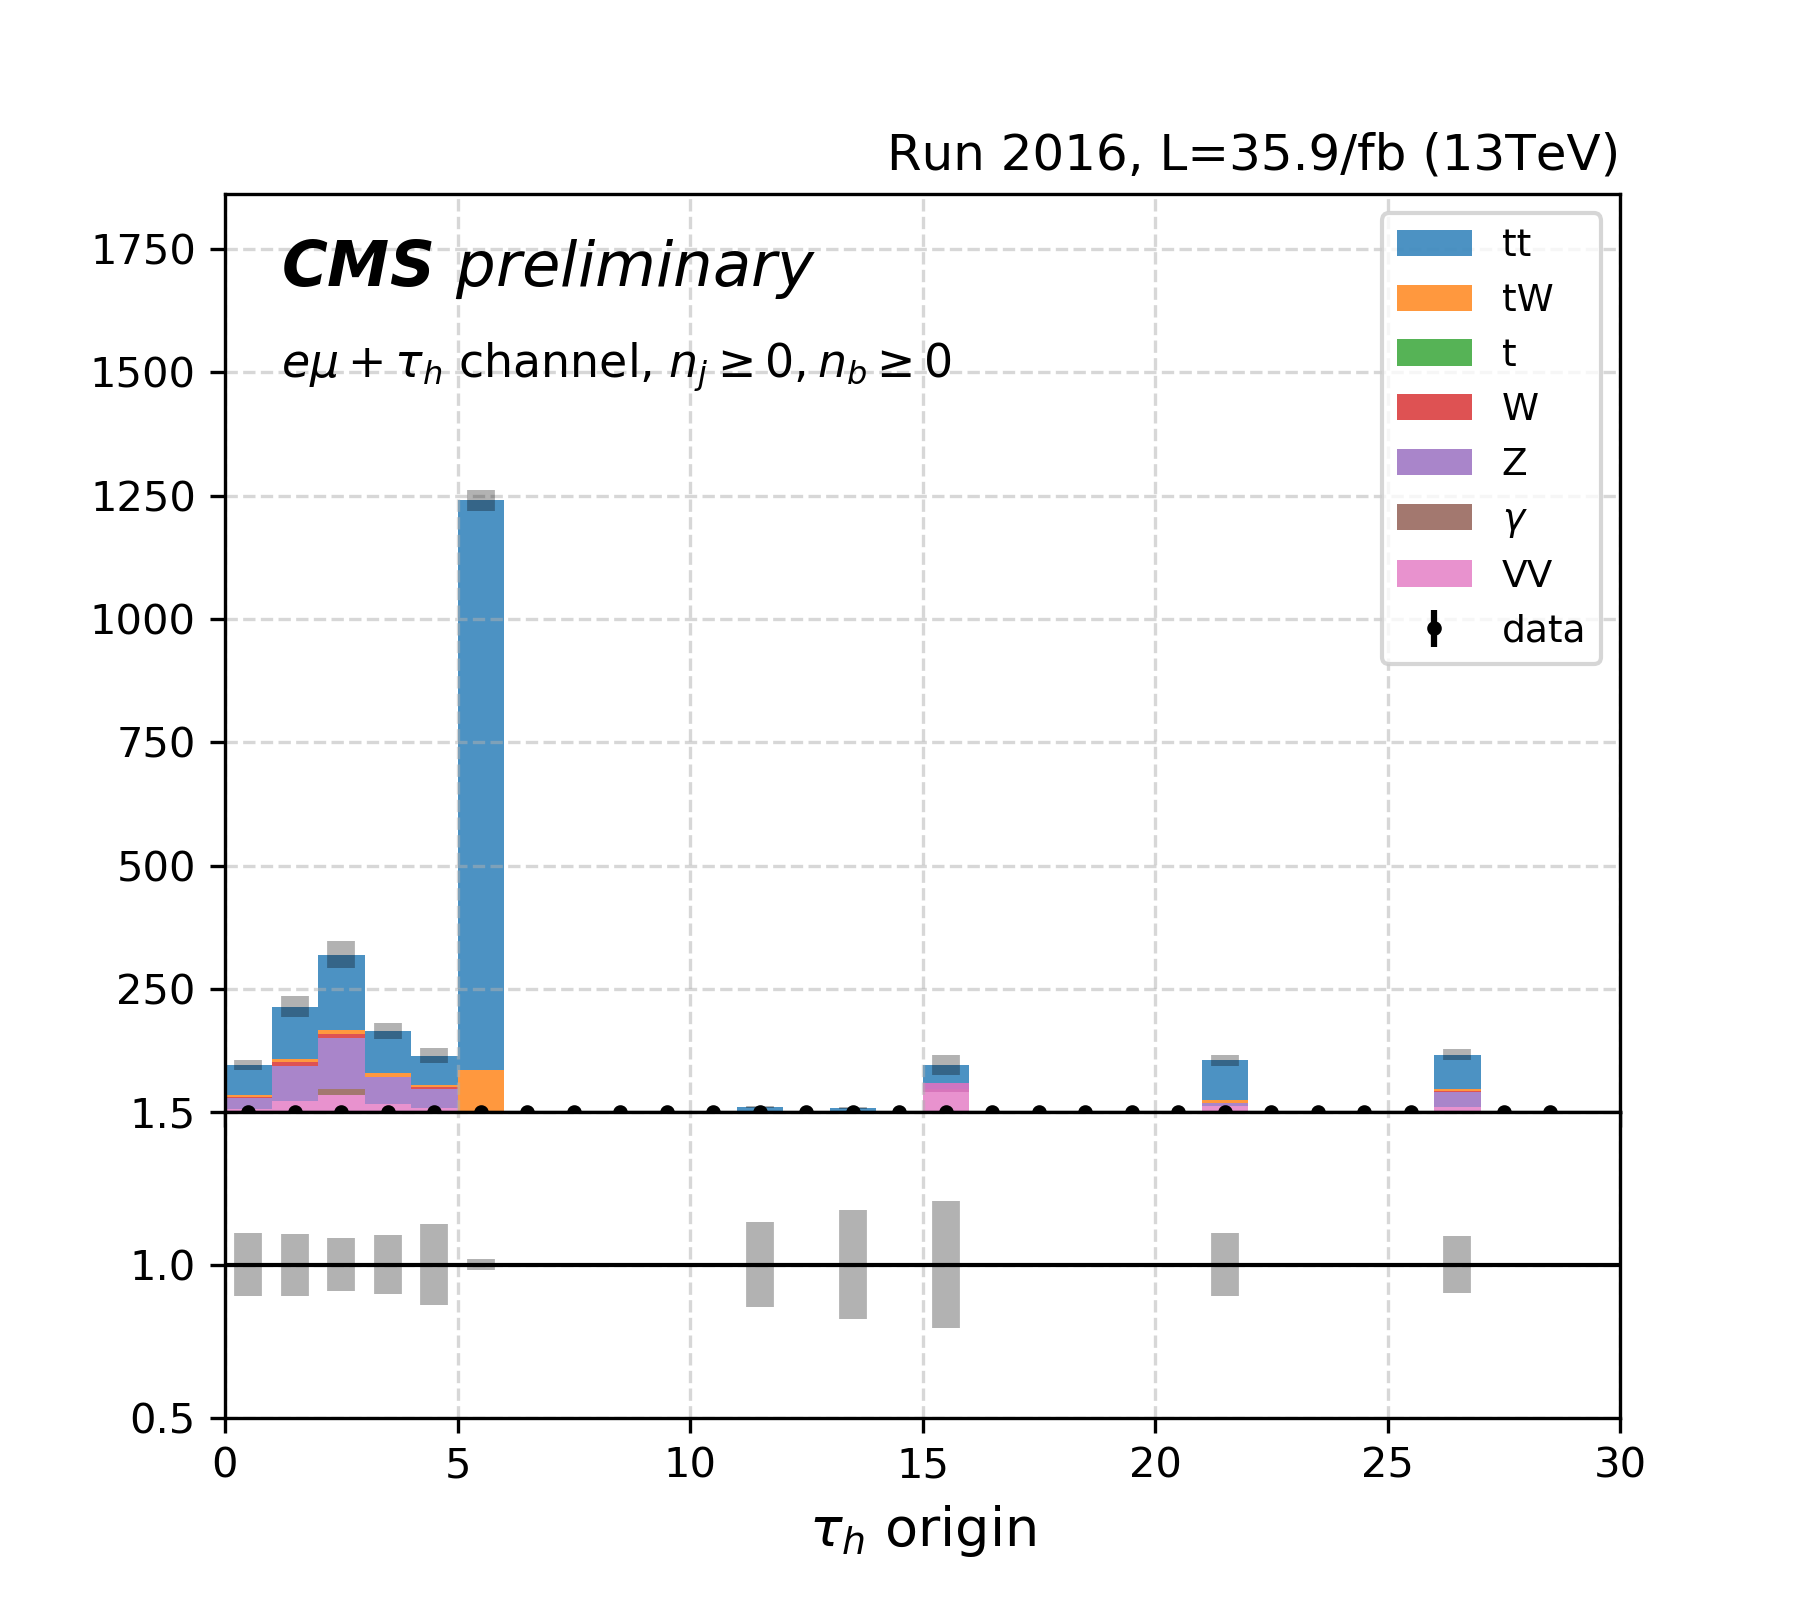
\includegraphics[width=0.4\textwidth]{chapters/Appendix/sectionJetToTauh/figures/emutau_tauGenFlavor_pickles_lltauTight.png}
    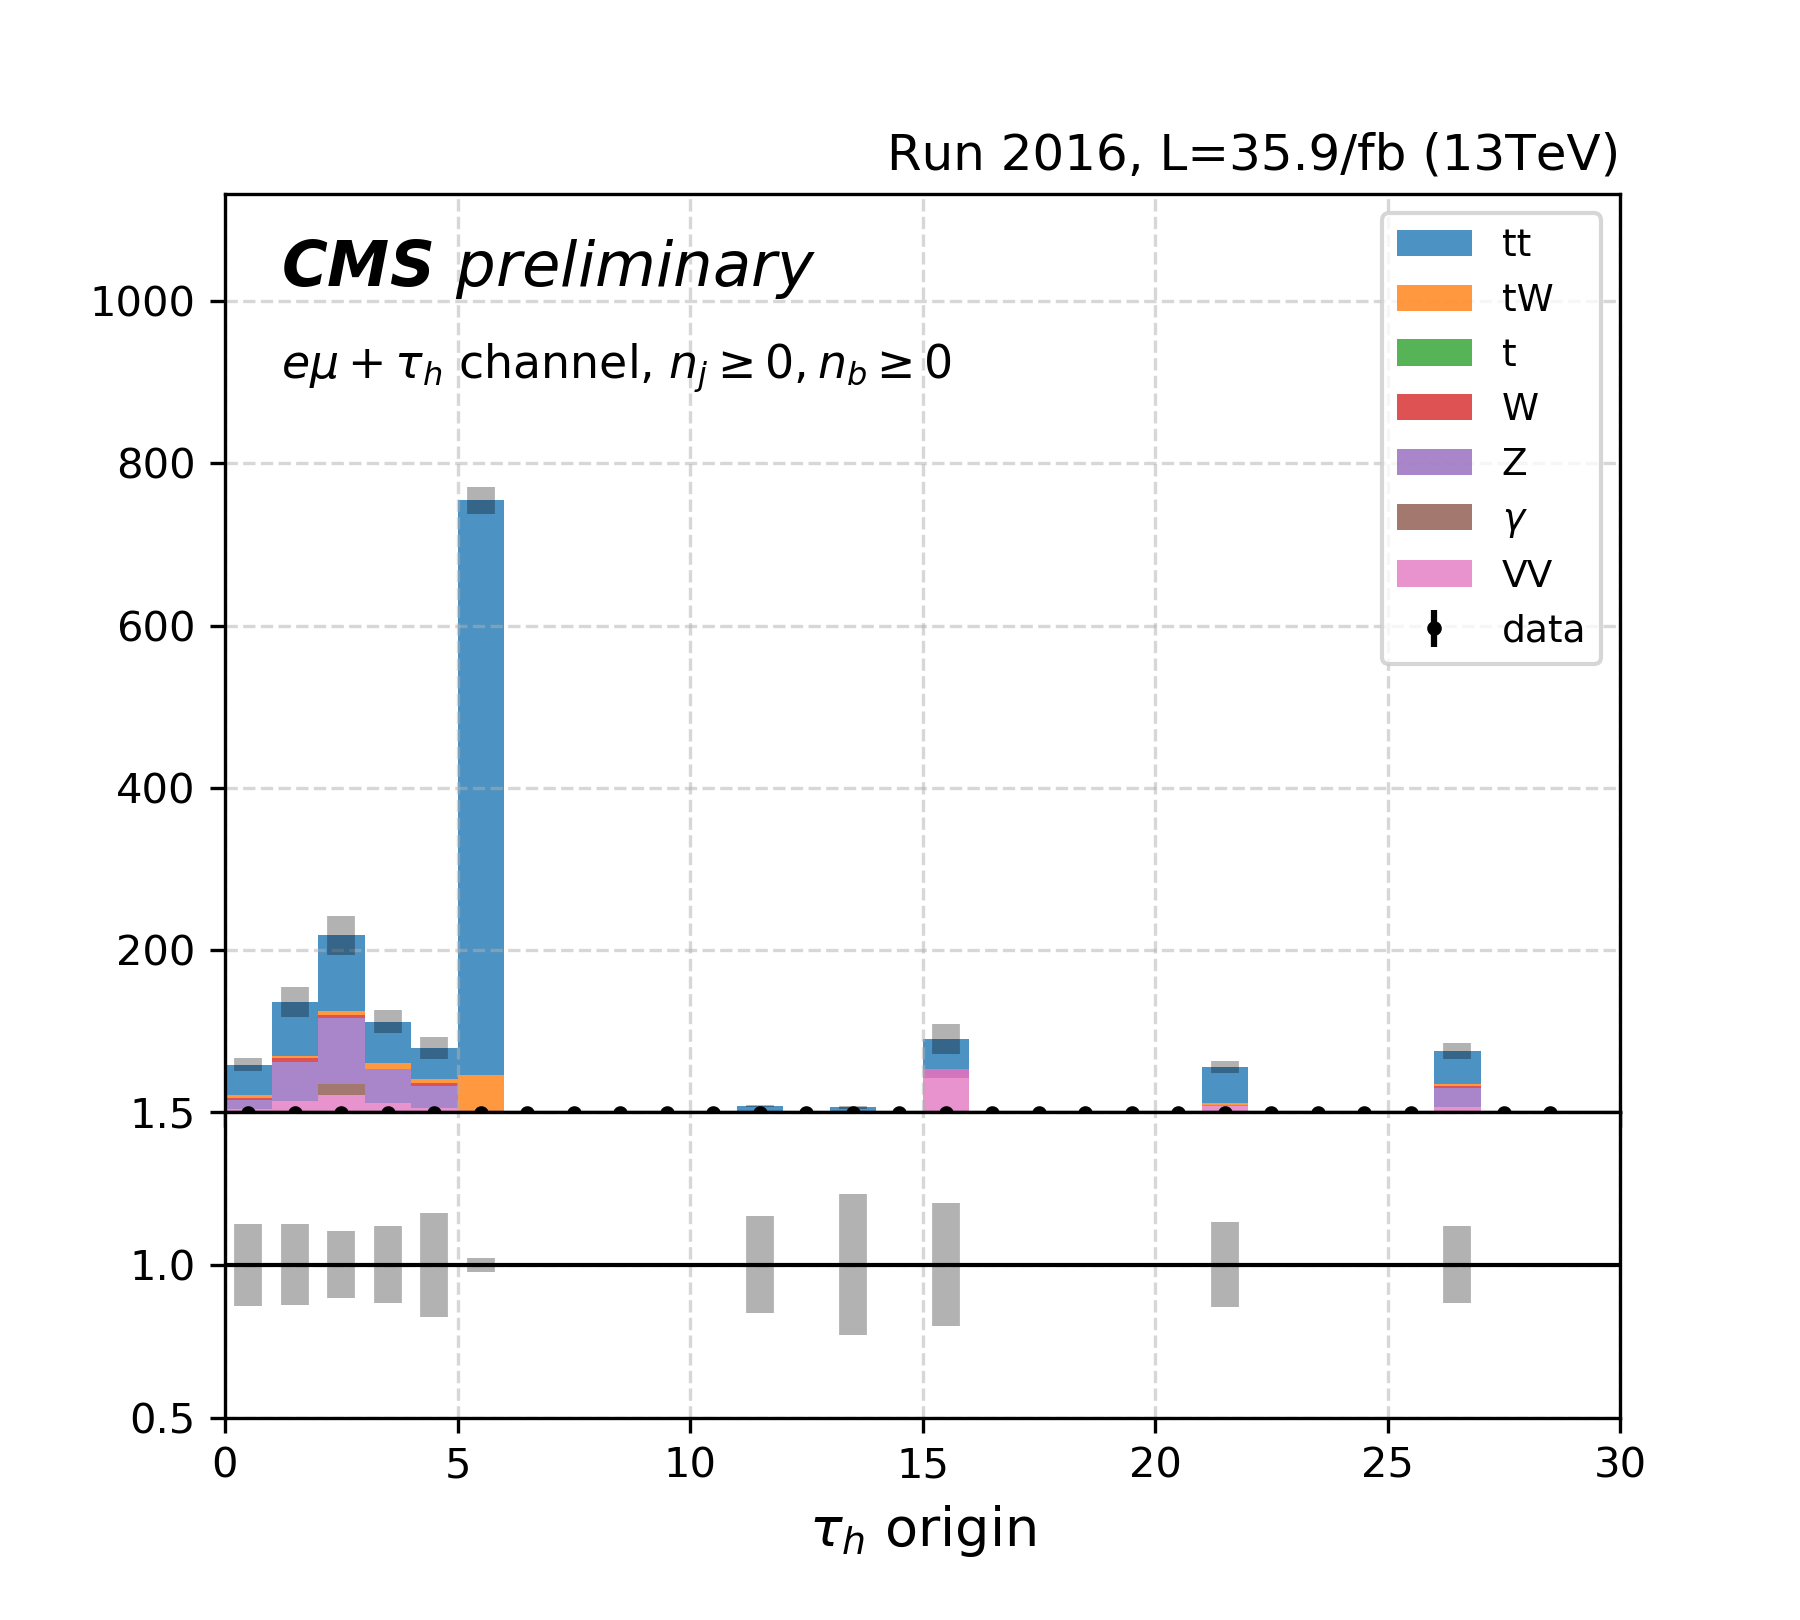
\includegraphics[width=0.4\textwidth]{chapters/Appendix/sectionJetToTauh/figures/emutau_tauGenFlavor_pickles_lltauVTight.png}
    \caption{Distributions of $m_{e\mu}$, $\tau pT$ and gen-level $\tau_h$ origin in the $e\mu+\tau$ channel. The left and right column shows the Tight and VTight $\tau_h$ WP respectively.}
    \label{fig:appendix:fakeTauId:emutau}
\end{figure}

\begin{figure}
    \centering
    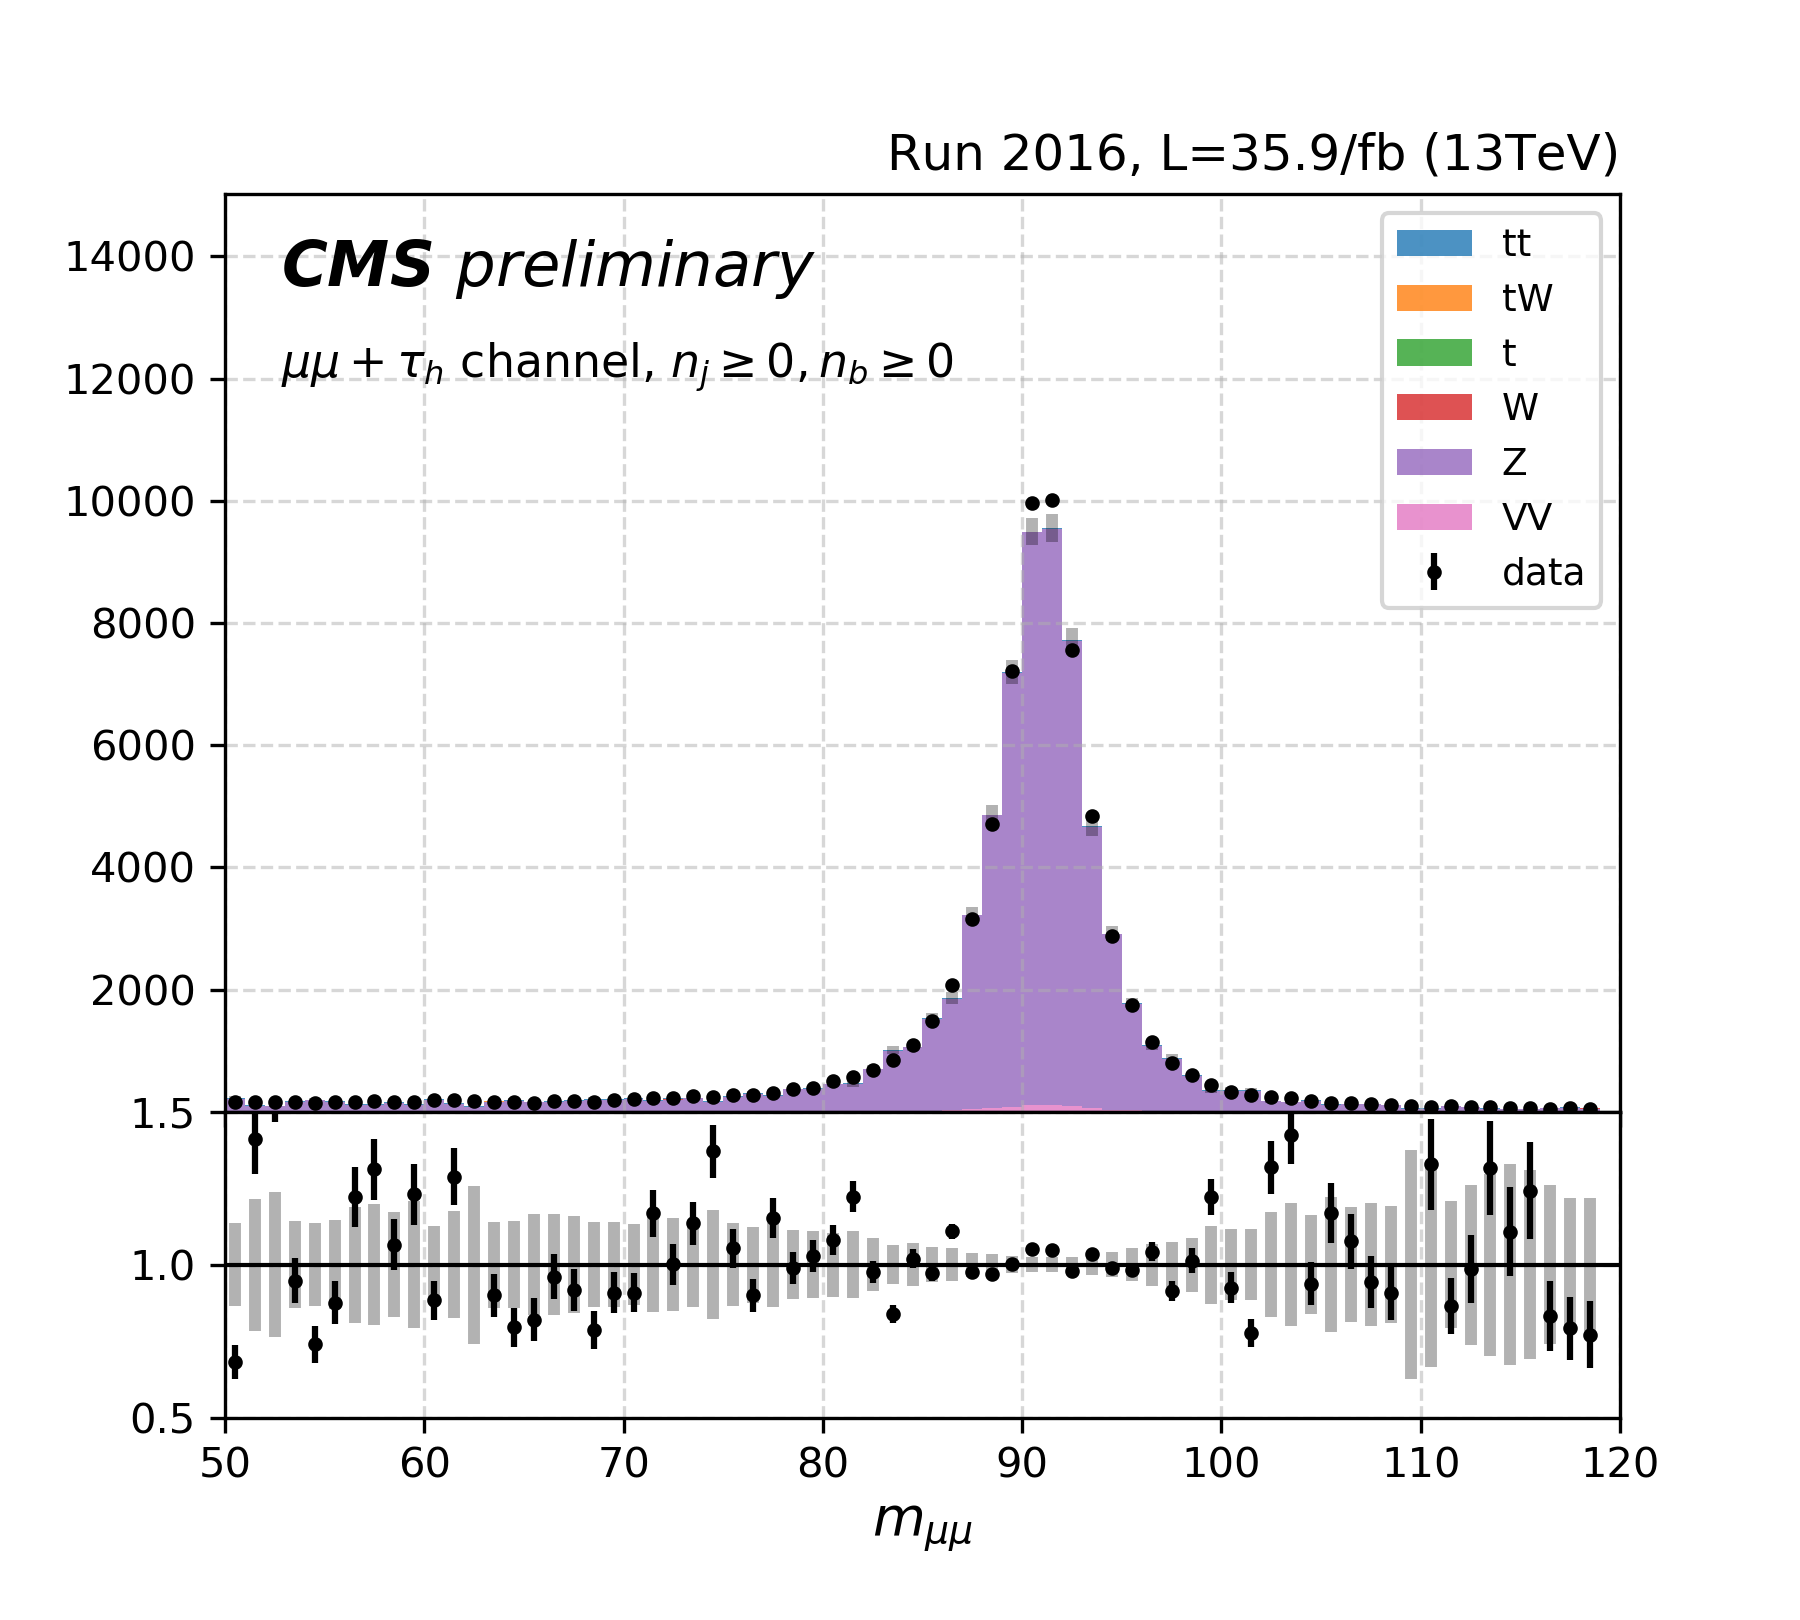
\includegraphics[width=0.4\textwidth]{chapters/Appendix/sectionJetToTauh/figures/mumutau_dilepton_mass_pickles_lltauTight.png}
    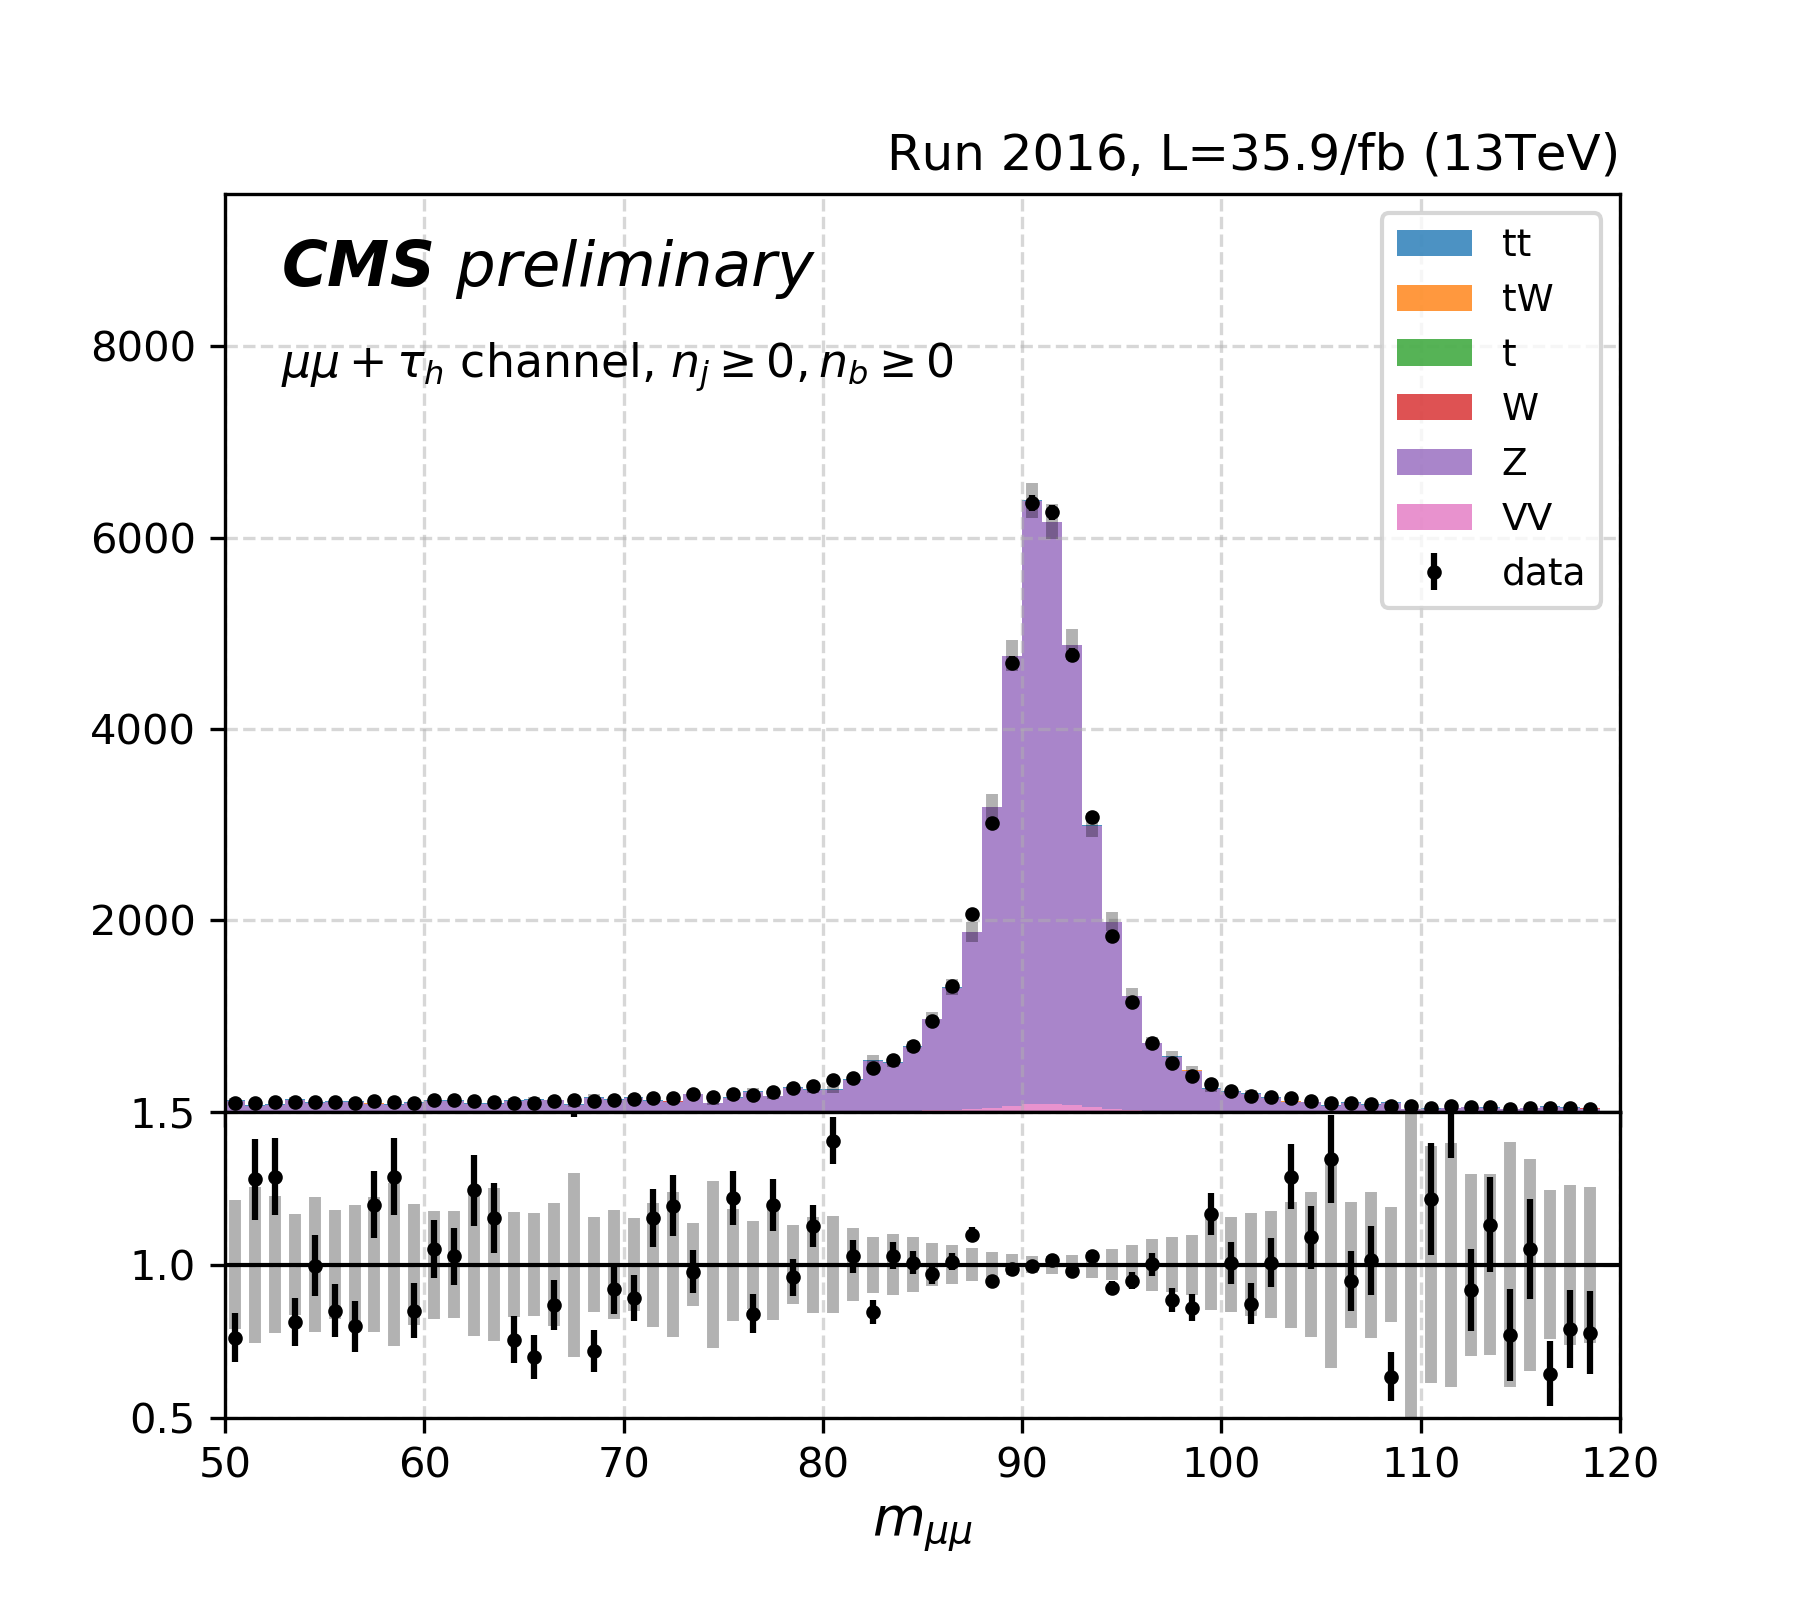
\includegraphics[width=0.4\textwidth]{chapters/Appendix/sectionJetToTauh/figures/mumutau_dilepton_mass_pickles_lltauVTight.png}
    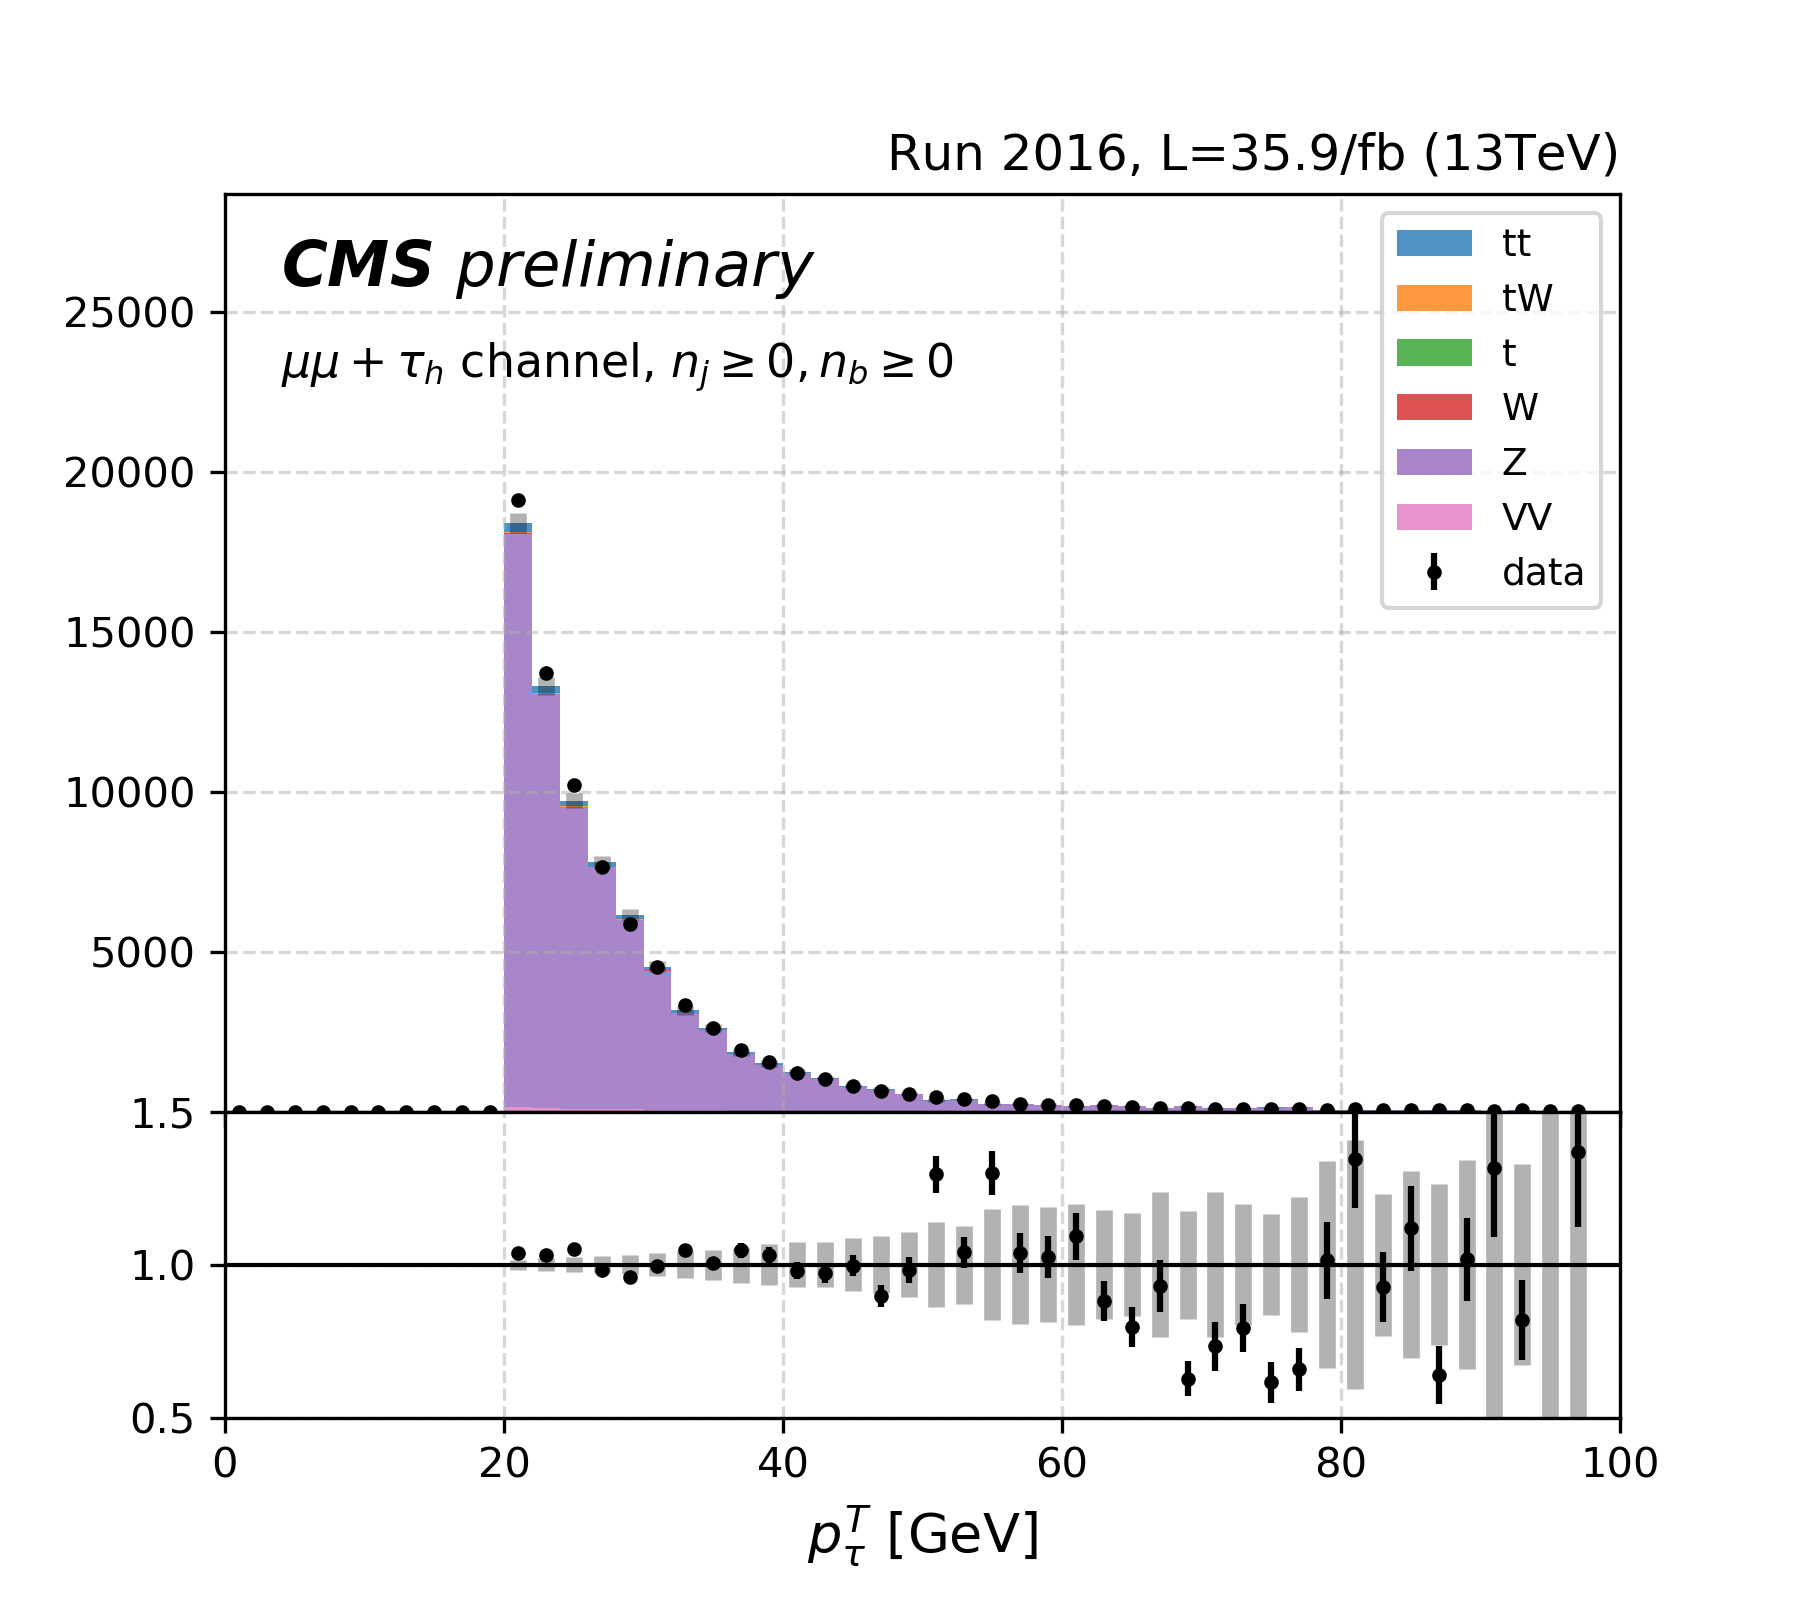
\includegraphics[width=0.4\textwidth]{chapters/Appendix/sectionJetToTauh/figures/mumutau_tauPt_pickles_lltauTight.png}
    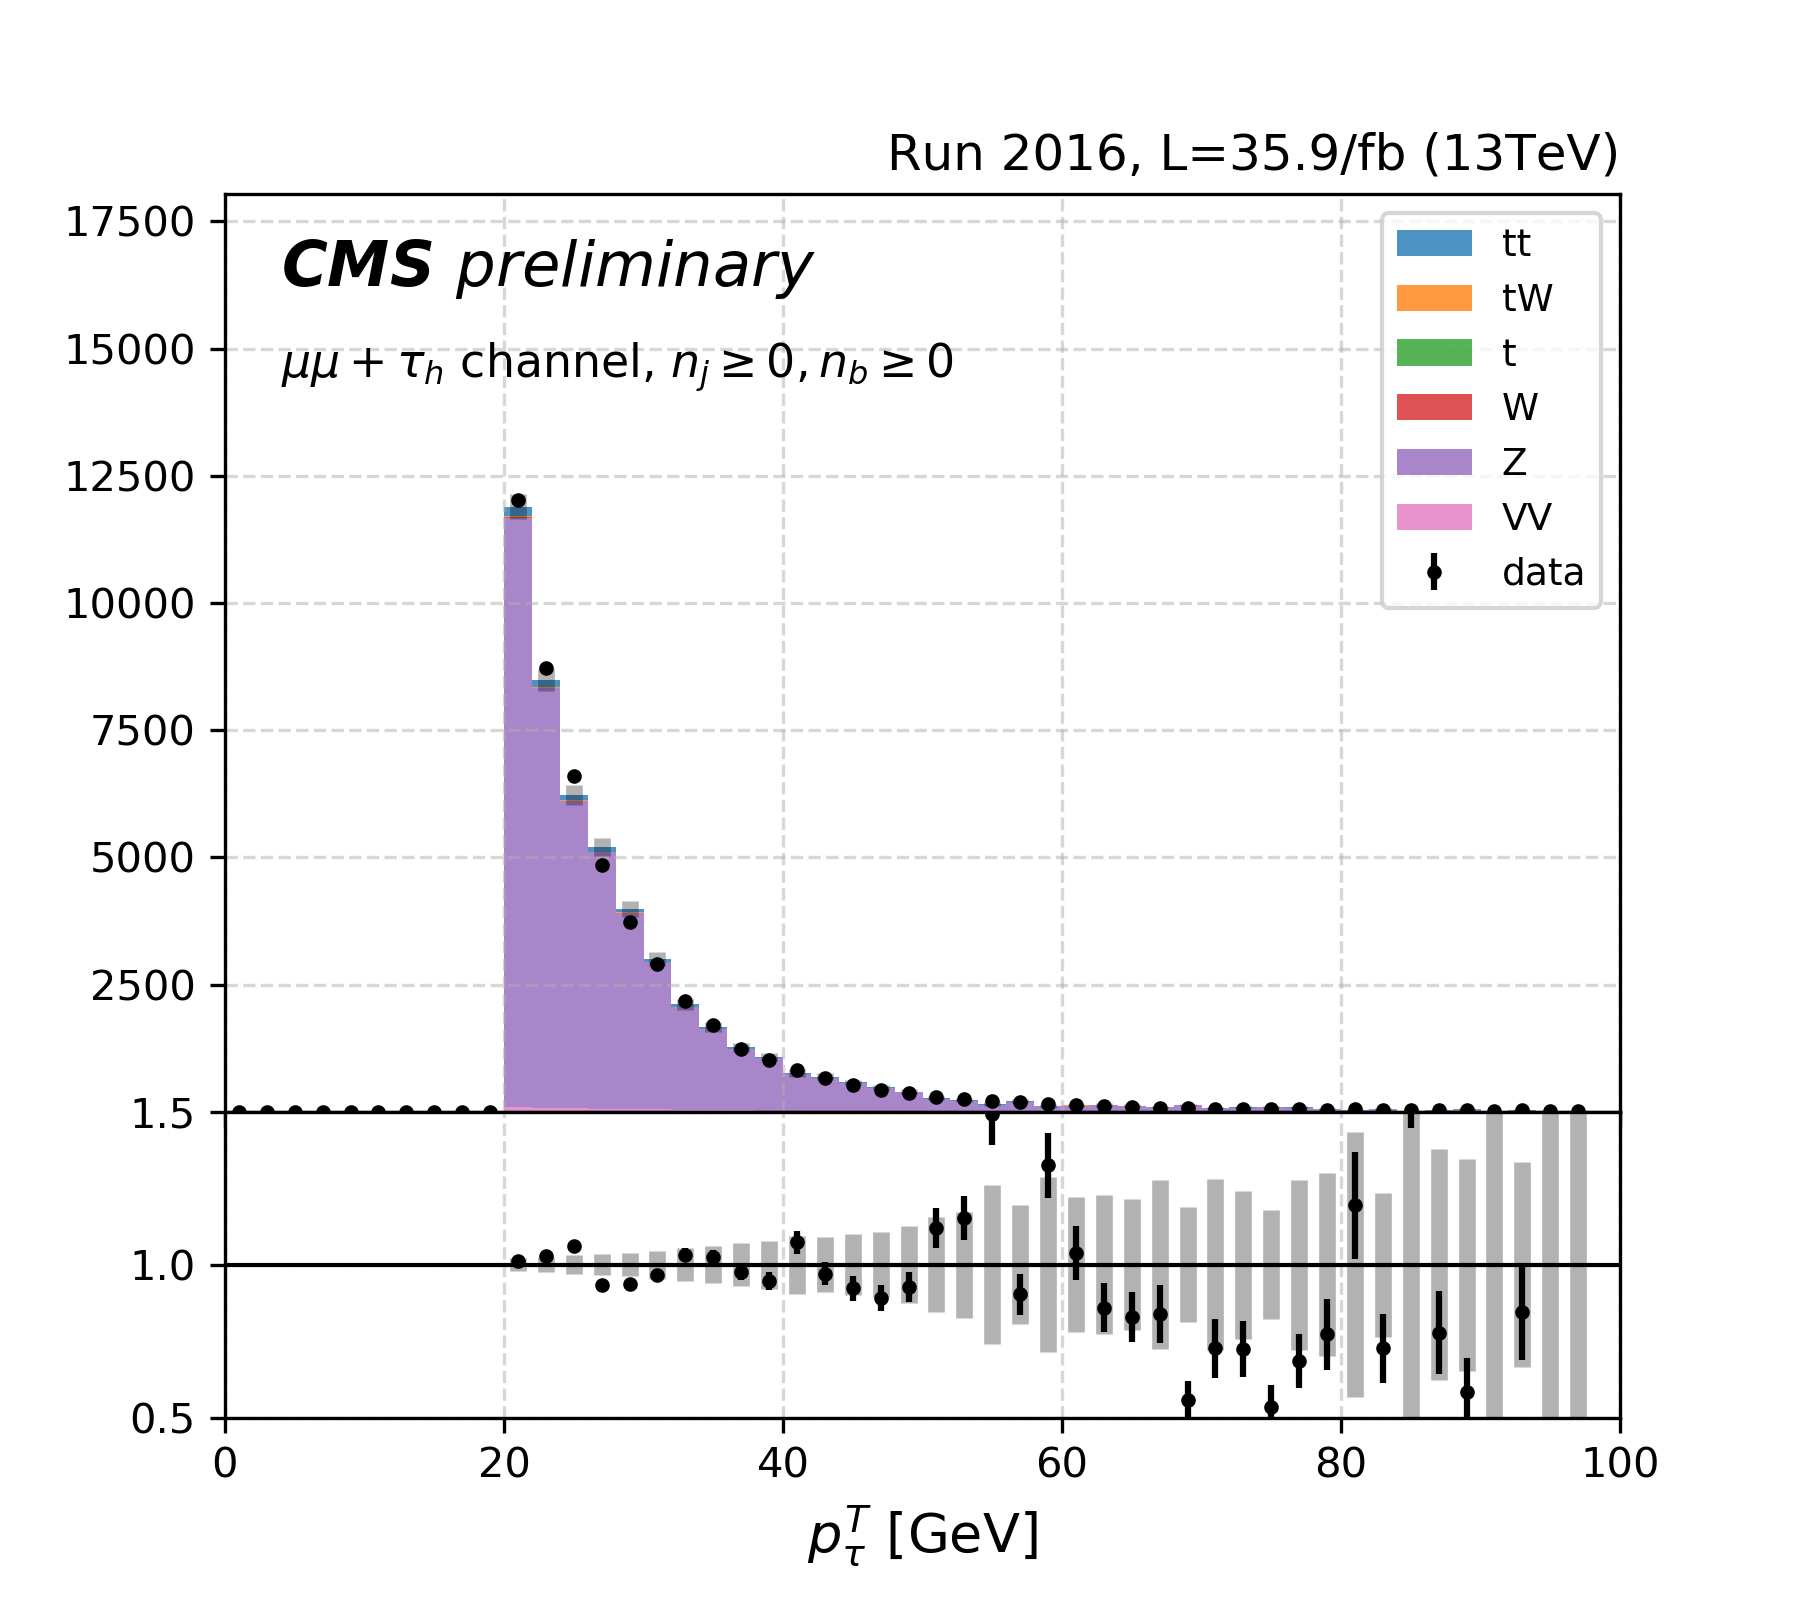
\includegraphics[width=0.4\textwidth]{chapters/Appendix/sectionJetToTauh/figures/mumutau_tauPt_pickles_lltauVTight.png}
    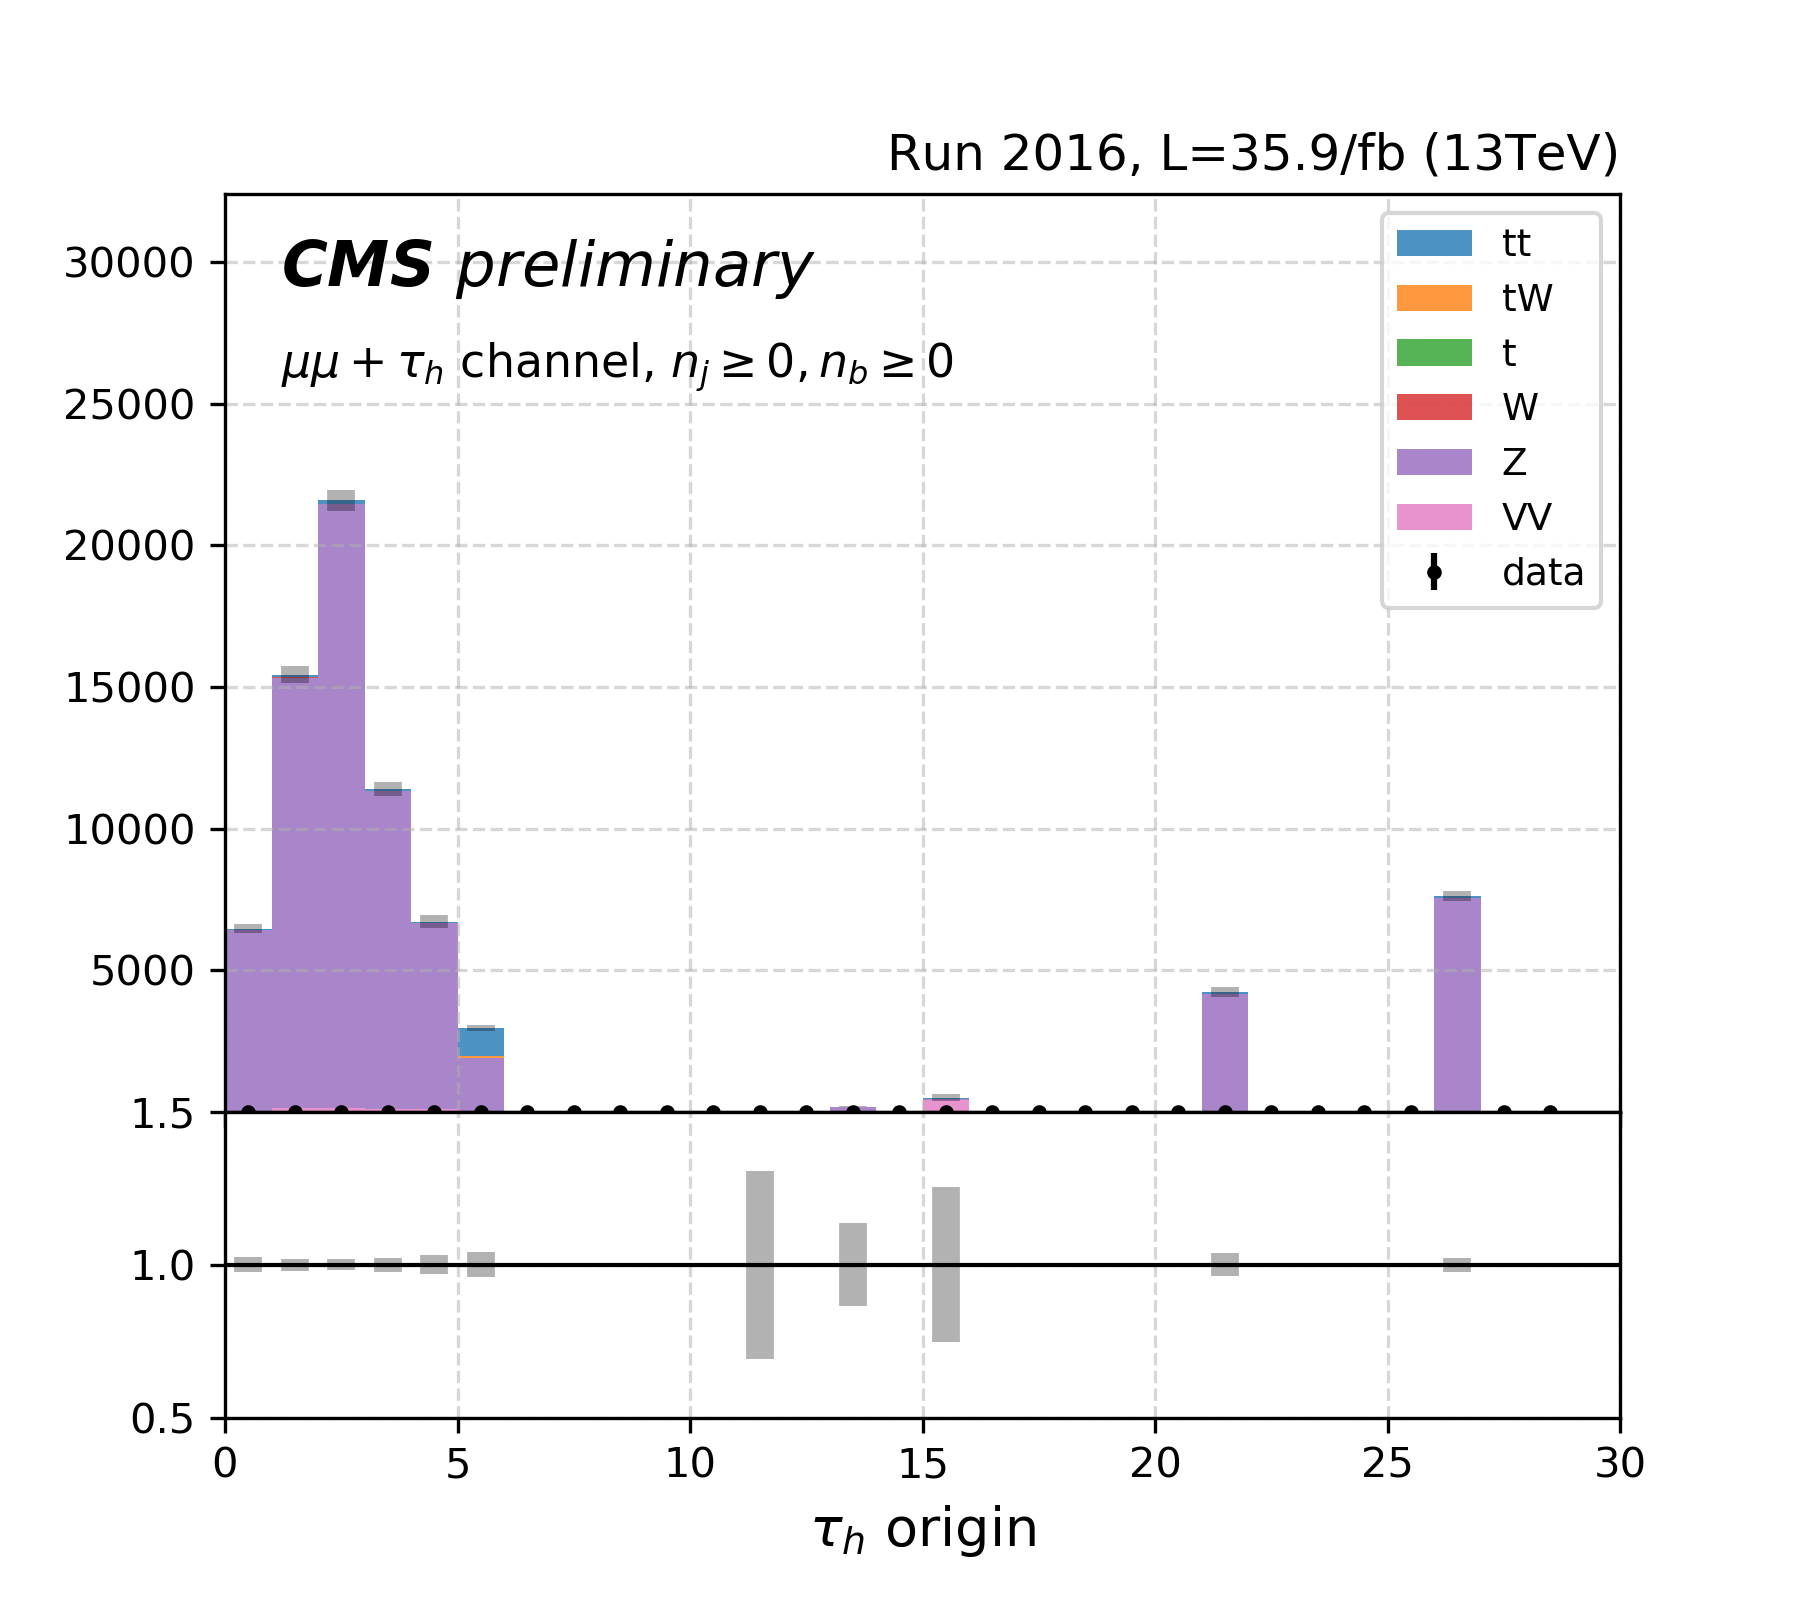
\includegraphics[width=0.4\textwidth]{chapters/Appendix/sectionJetToTauh/figures/mumutau_tauGenFlavor_pickles_lltauTight.png}
    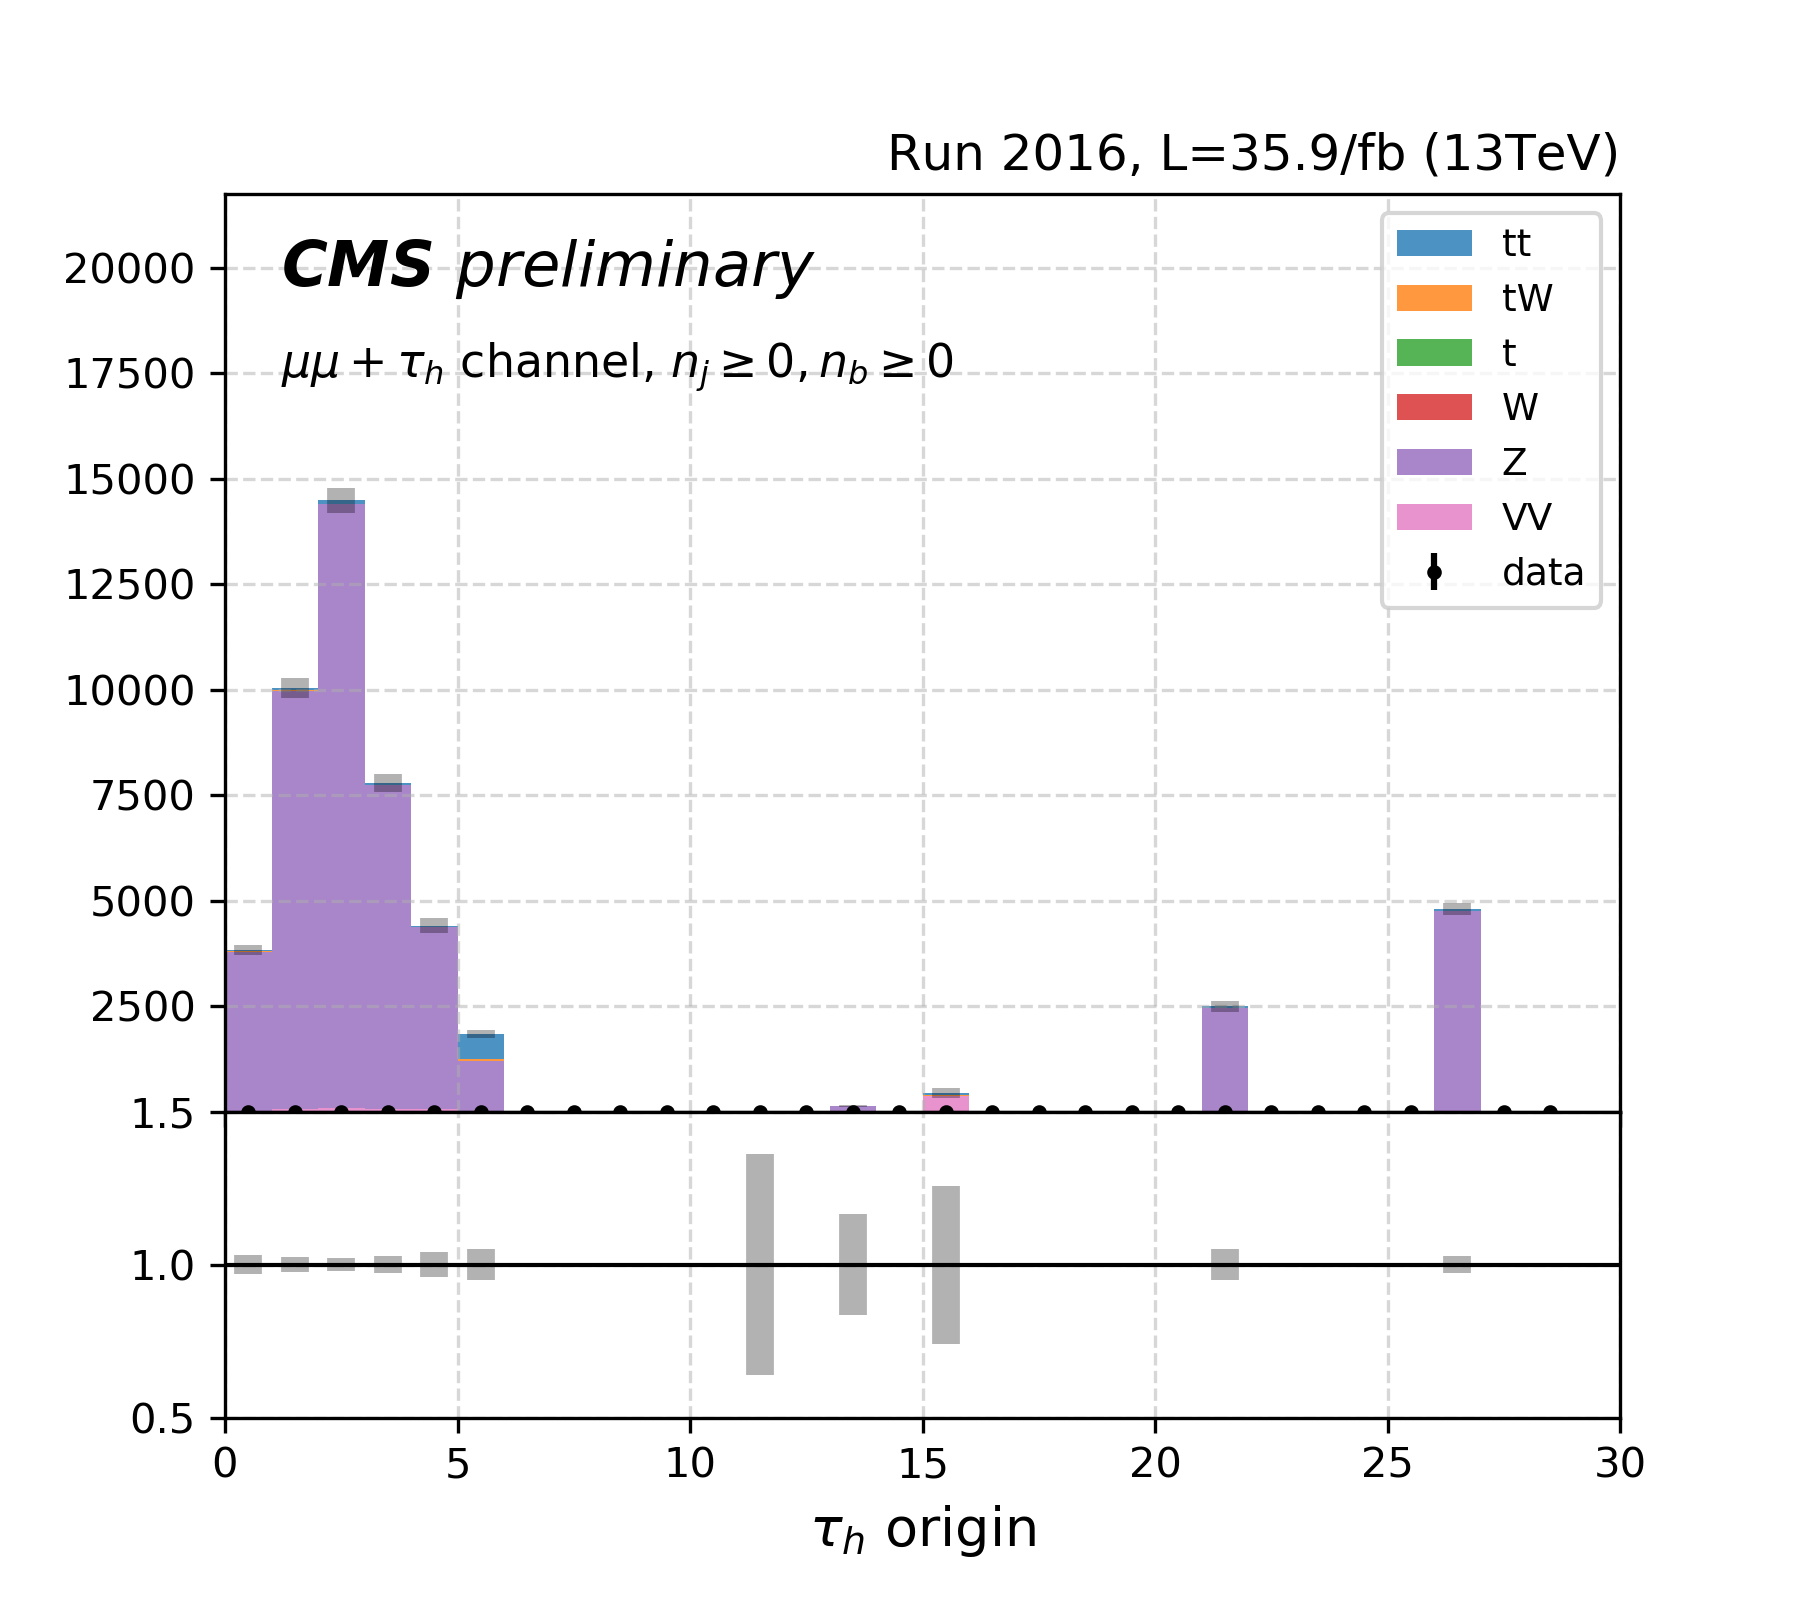
\includegraphics[width=0.4\textwidth]{chapters/Appendix/sectionJetToTauh/figures/mumutau_tauGenFlavor_pickles_lltauVTight.png}
    \caption{Distributions of $m_{\mu\mu}$, $\tau pT$ and gen-level $\tau_h$ origin in the $\mu\mu+\tau$ channel. The left and right column shows the Tight and VTight $\tau_h$ WP respectively.}
    \label{fig:appendix:fakeTauId:mumutau}
\end{figure}


\begin{figure}
    \centering
    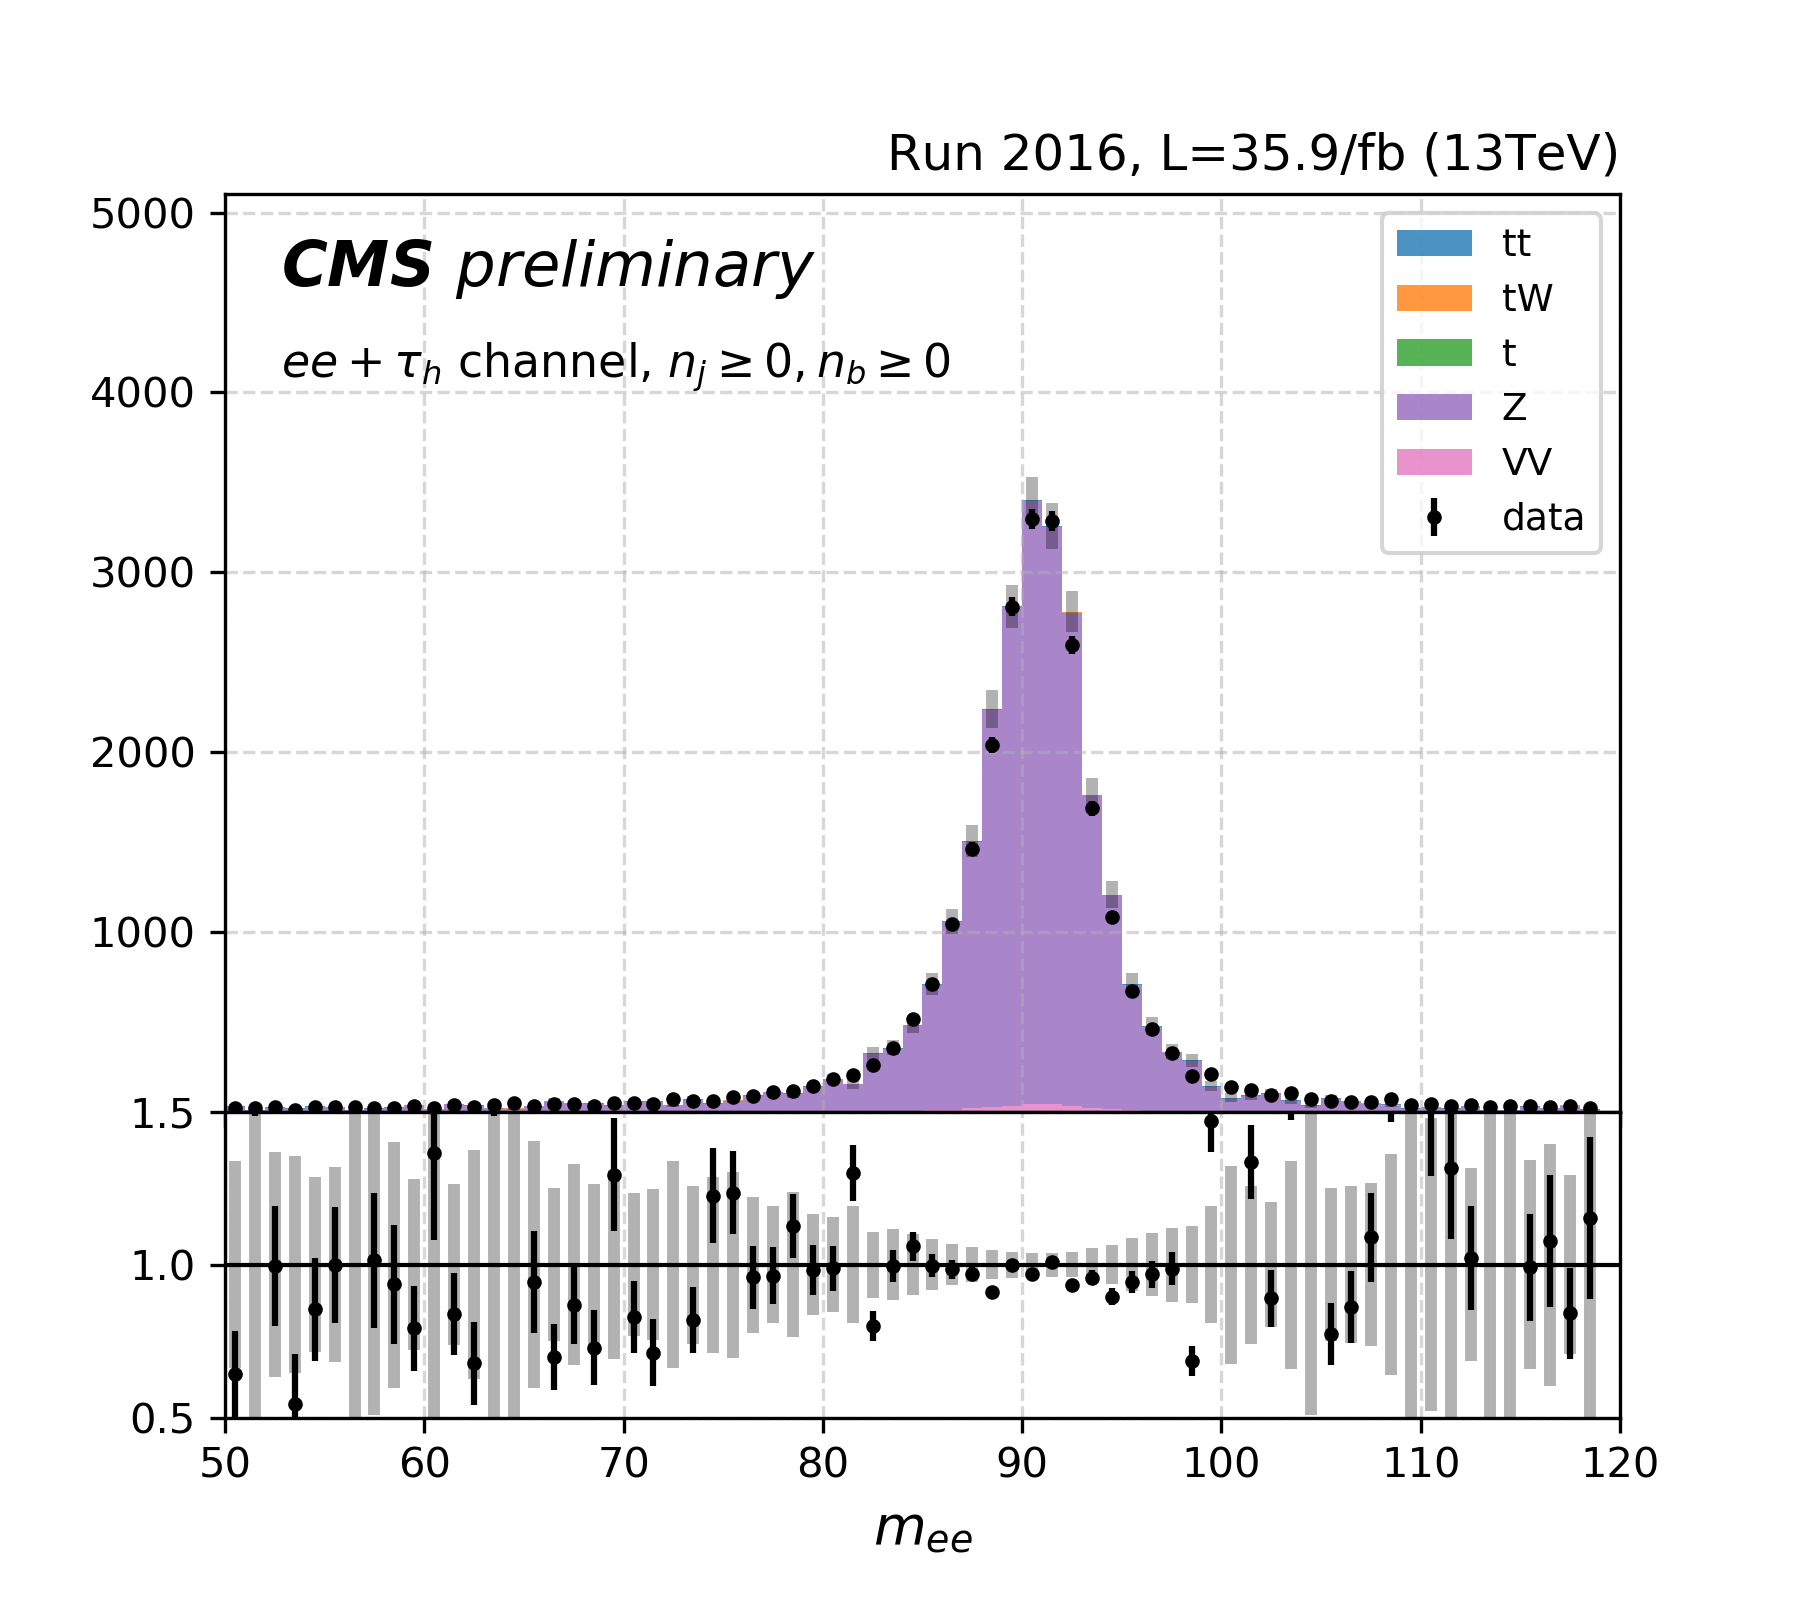
\includegraphics[width=0.4\textwidth]{chapters/Appendix/sectionJetToTauh/figures/eetau_dilepton_mass_pickles_lltauTight.png}
    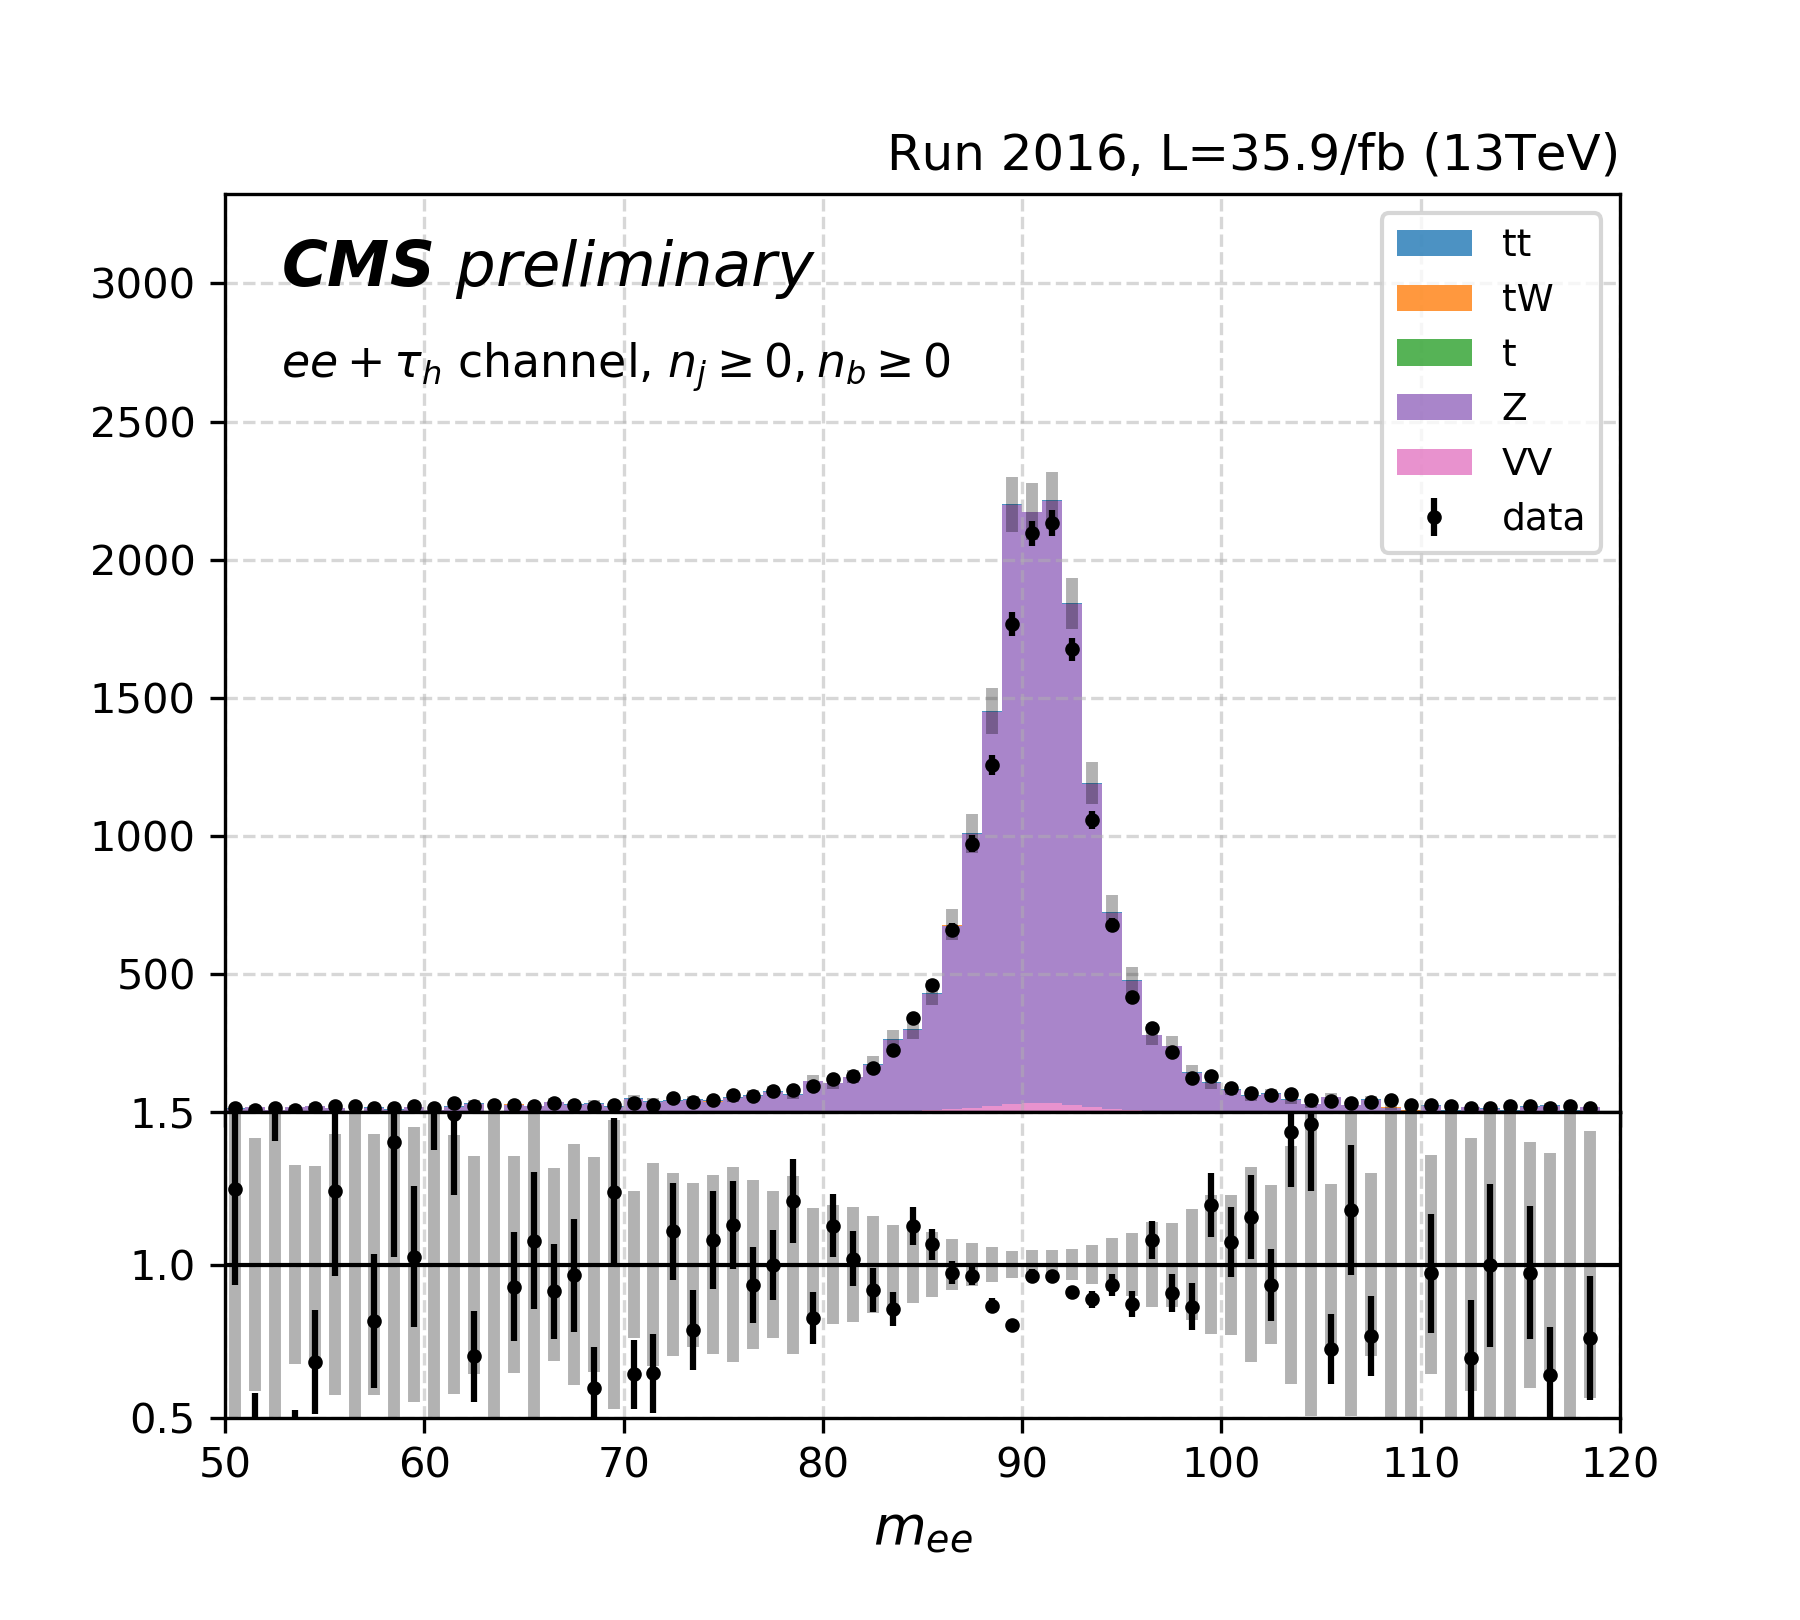
\includegraphics[width=0.4\textwidth]{chapters/Appendix/sectionJetToTauh/figures/eetau_dilepton_mass_pickles_lltauVTight.png}
    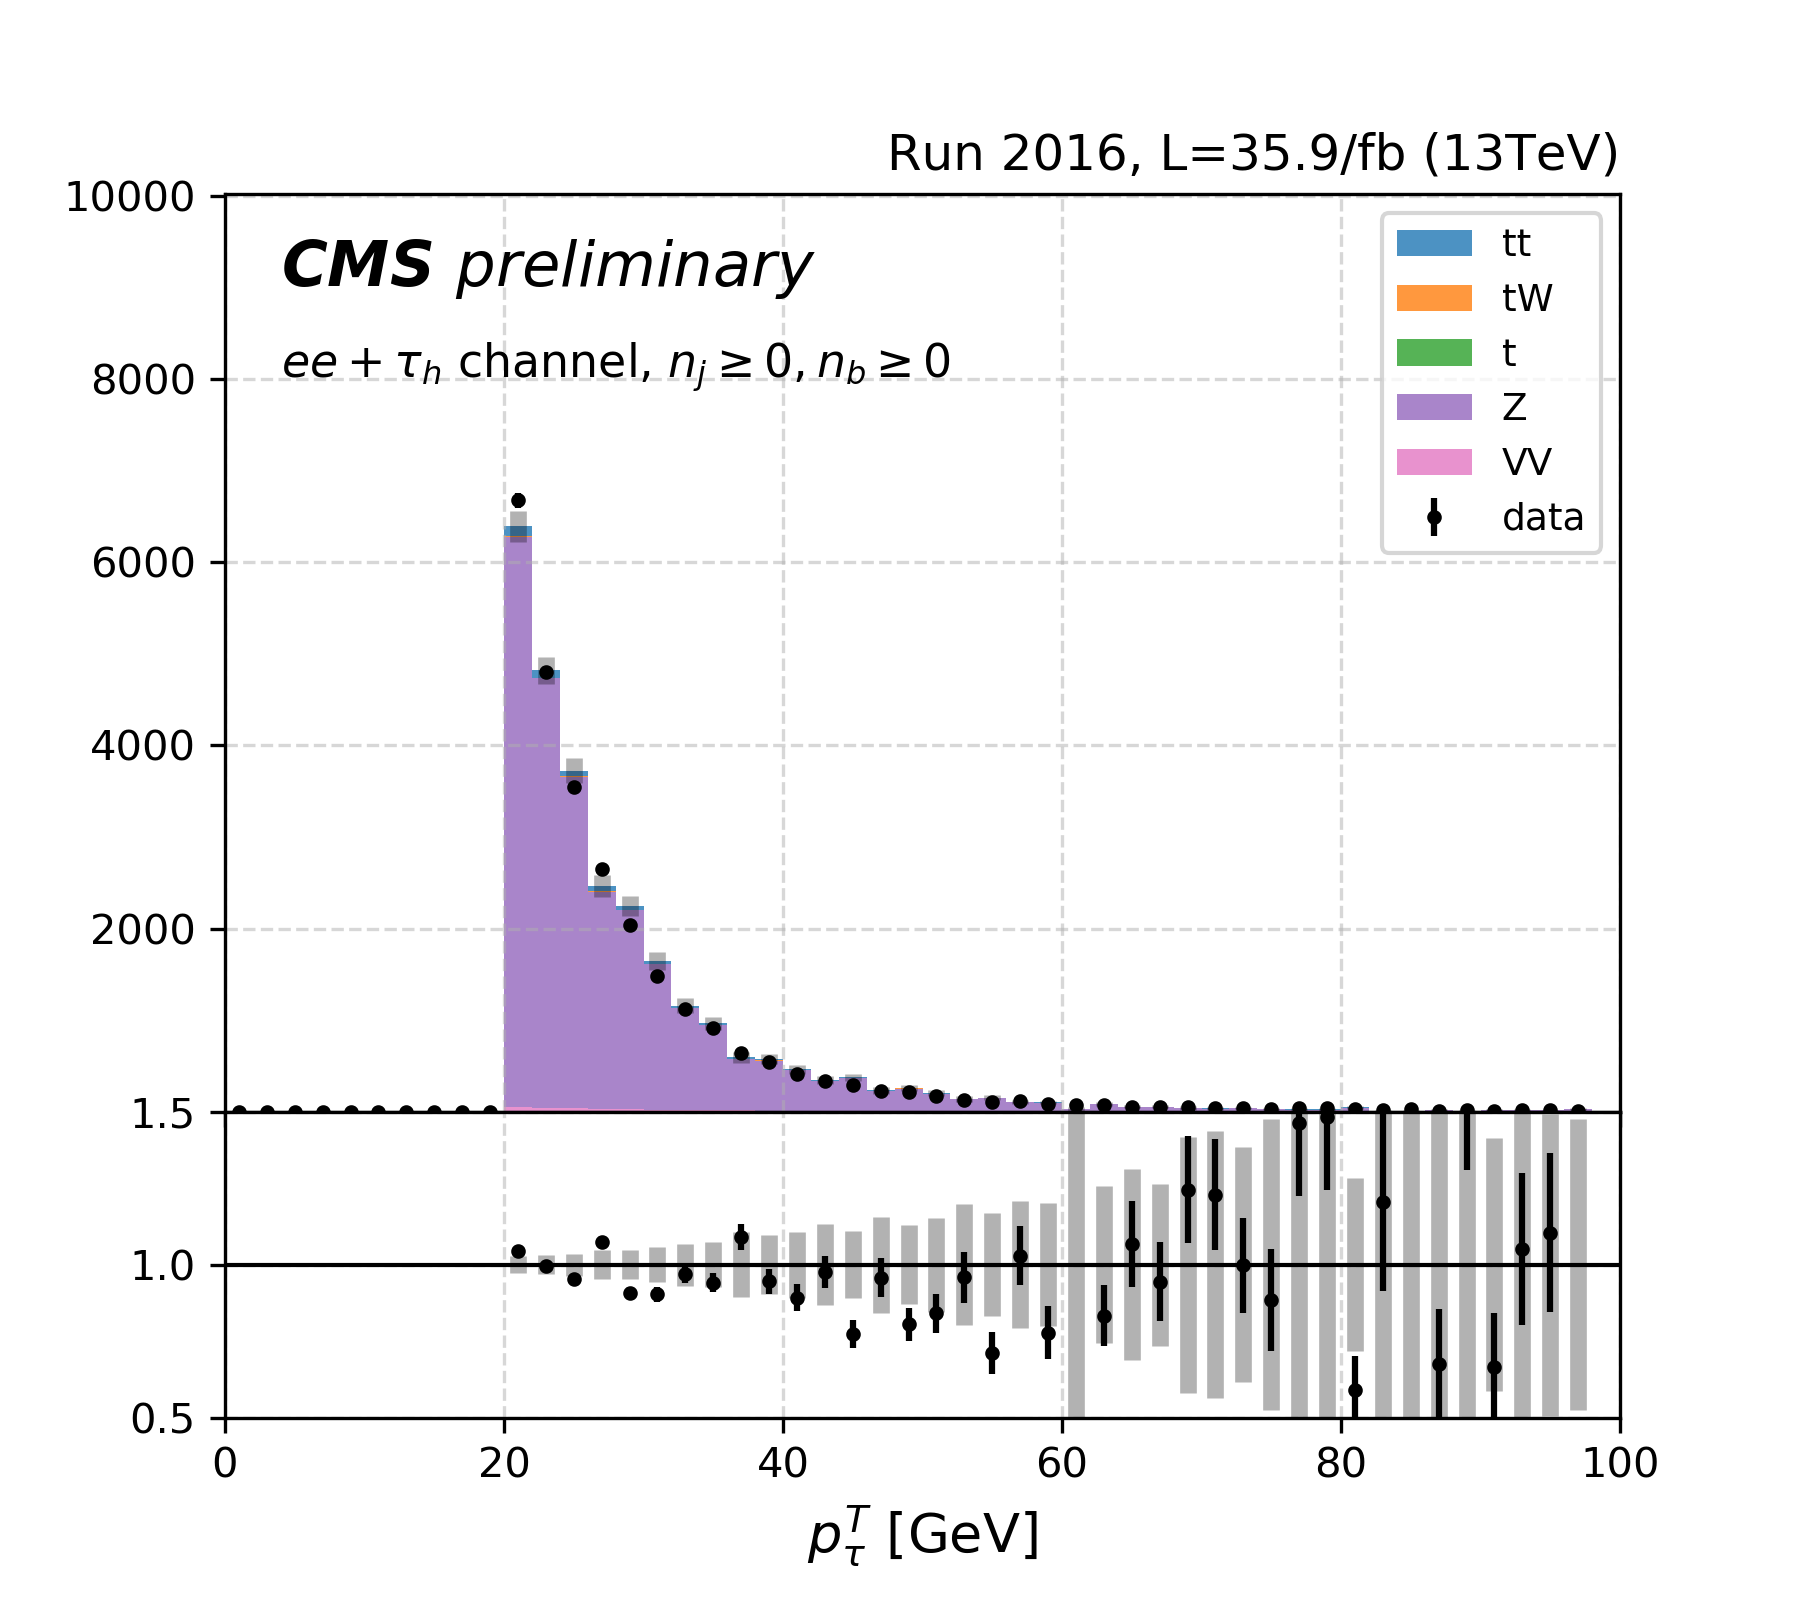
\includegraphics[width=0.4\textwidth]{chapters/Appendix/sectionJetToTauh/figures/eetau_tauPt_pickles_lltauTight.png}
    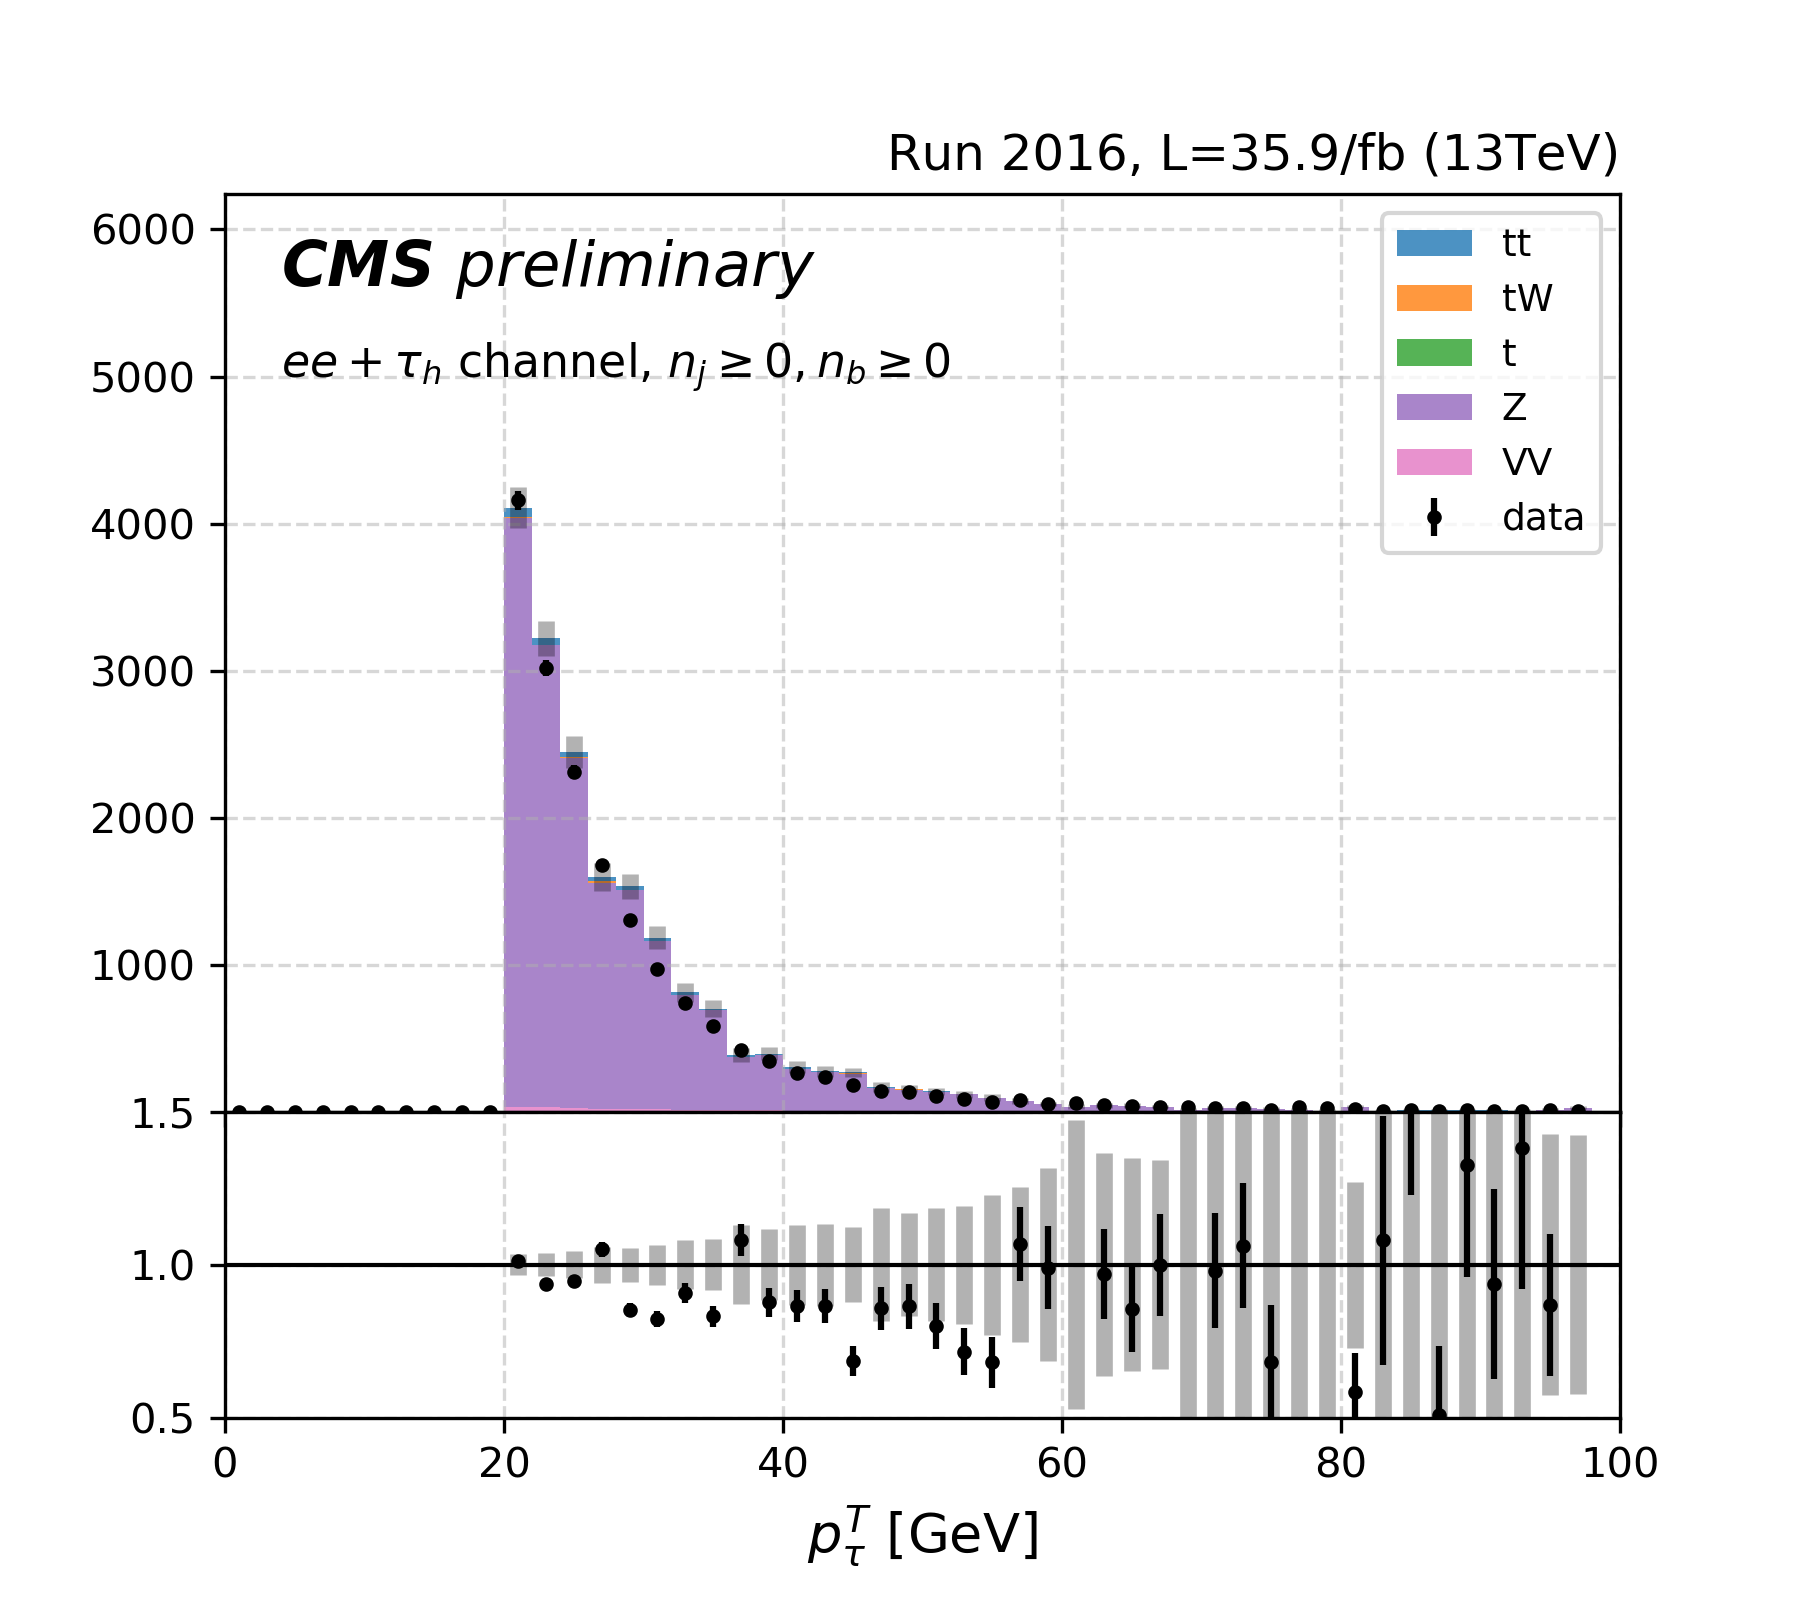
\includegraphics[width=0.4\textwidth]{chapters/Appendix/sectionJetToTauh/figures/eetau_tauPt_pickles_lltauVTight.png}
    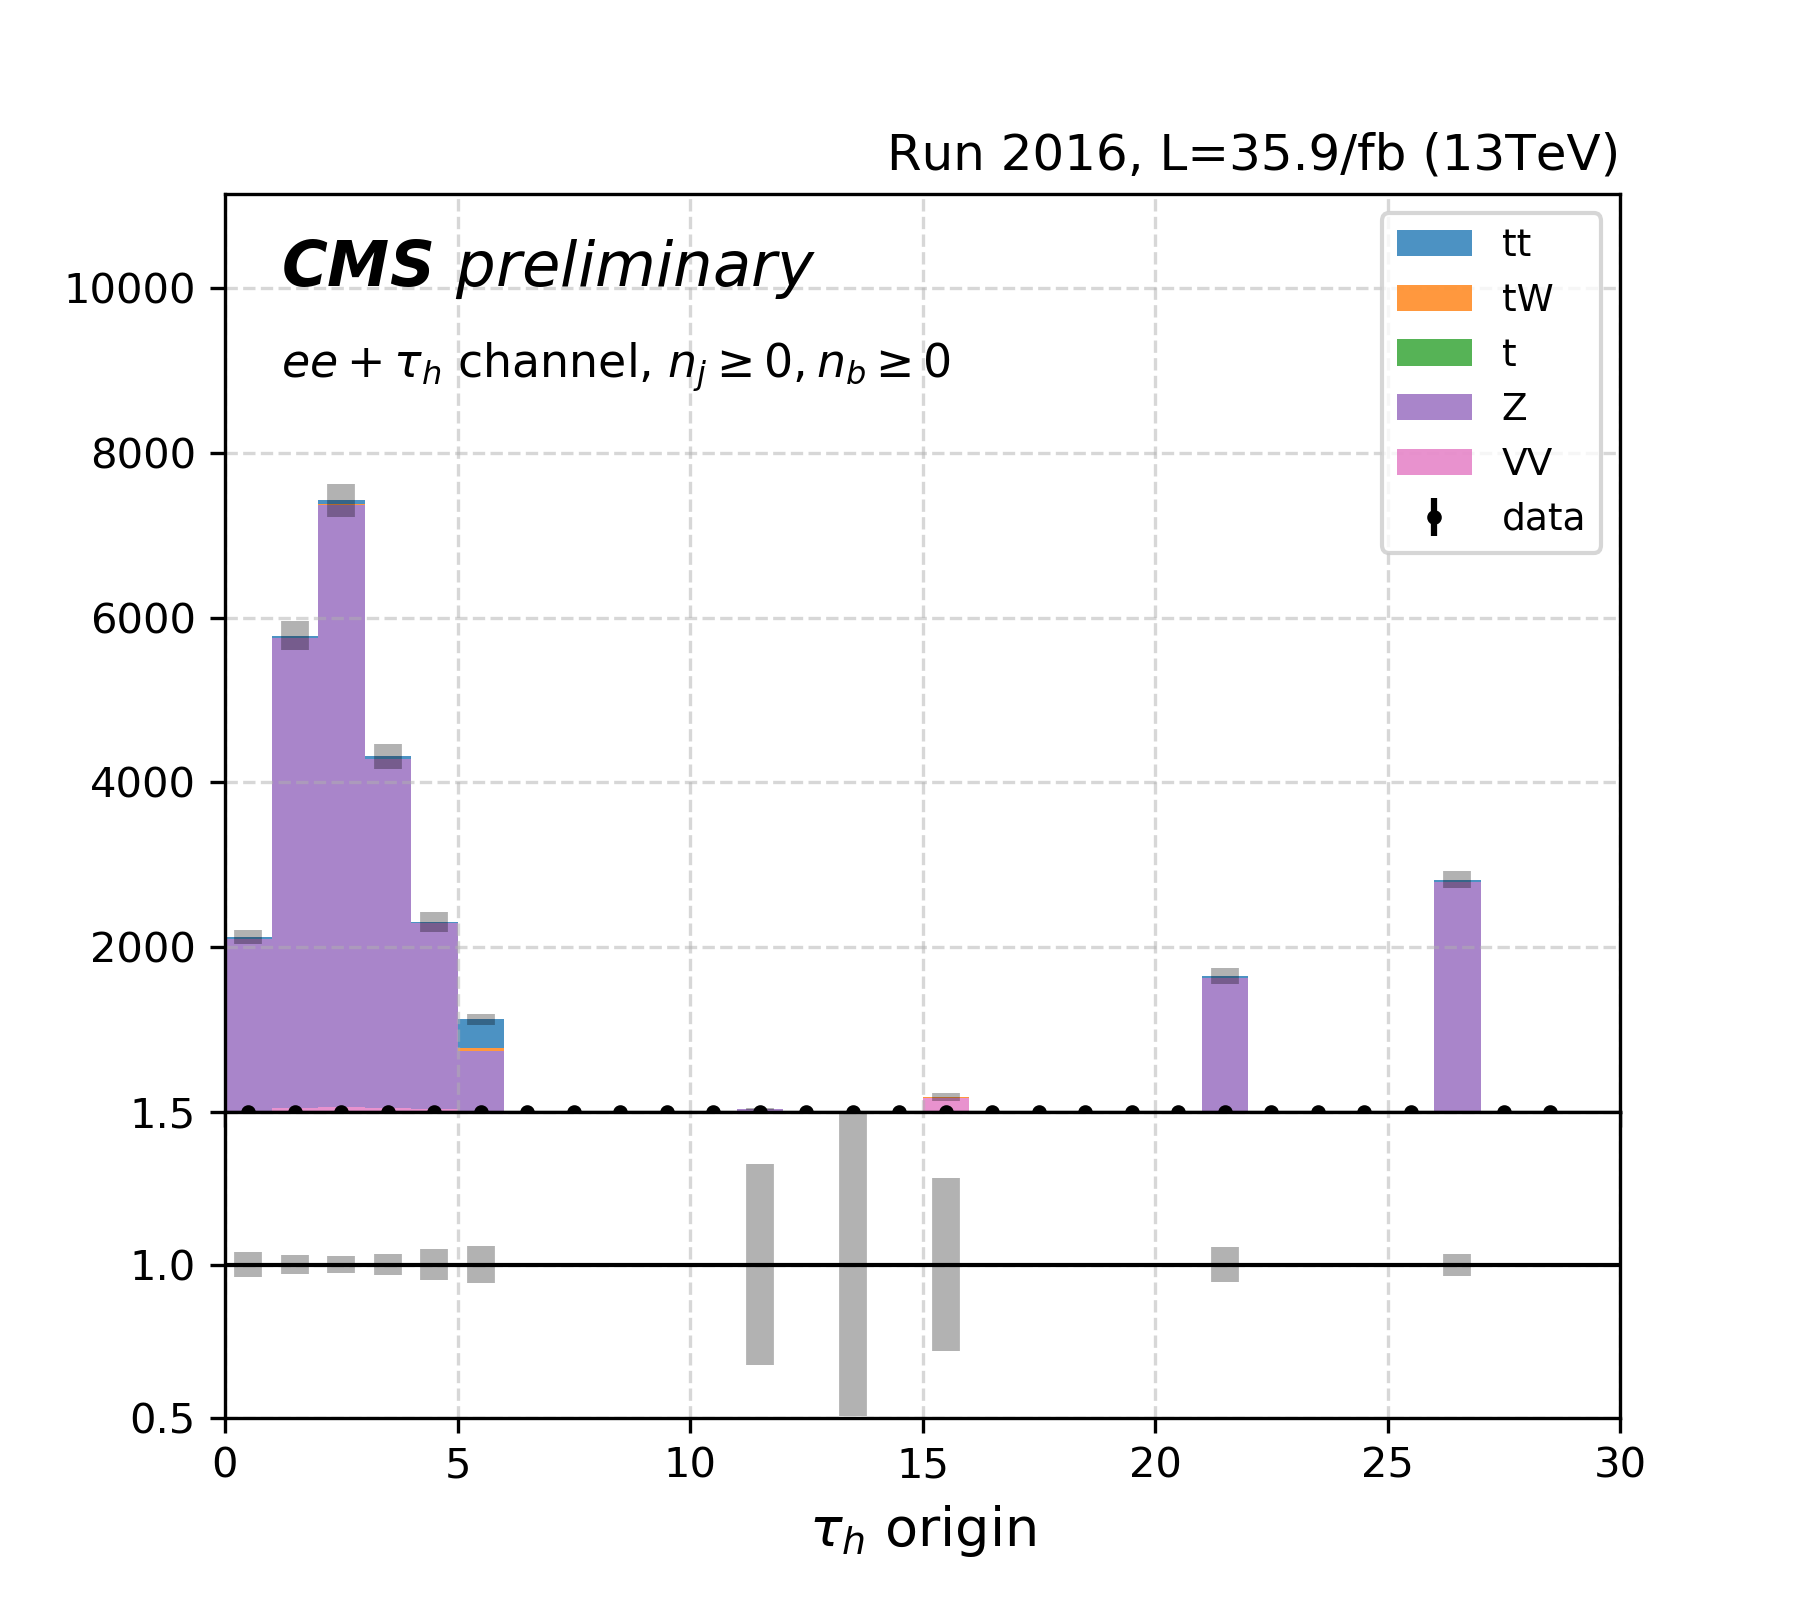
\includegraphics[width=0.4\textwidth]{chapters/Appendix/sectionJetToTauh/figures/eetau_tauGenFlavor_pickles_lltauTight.png}
    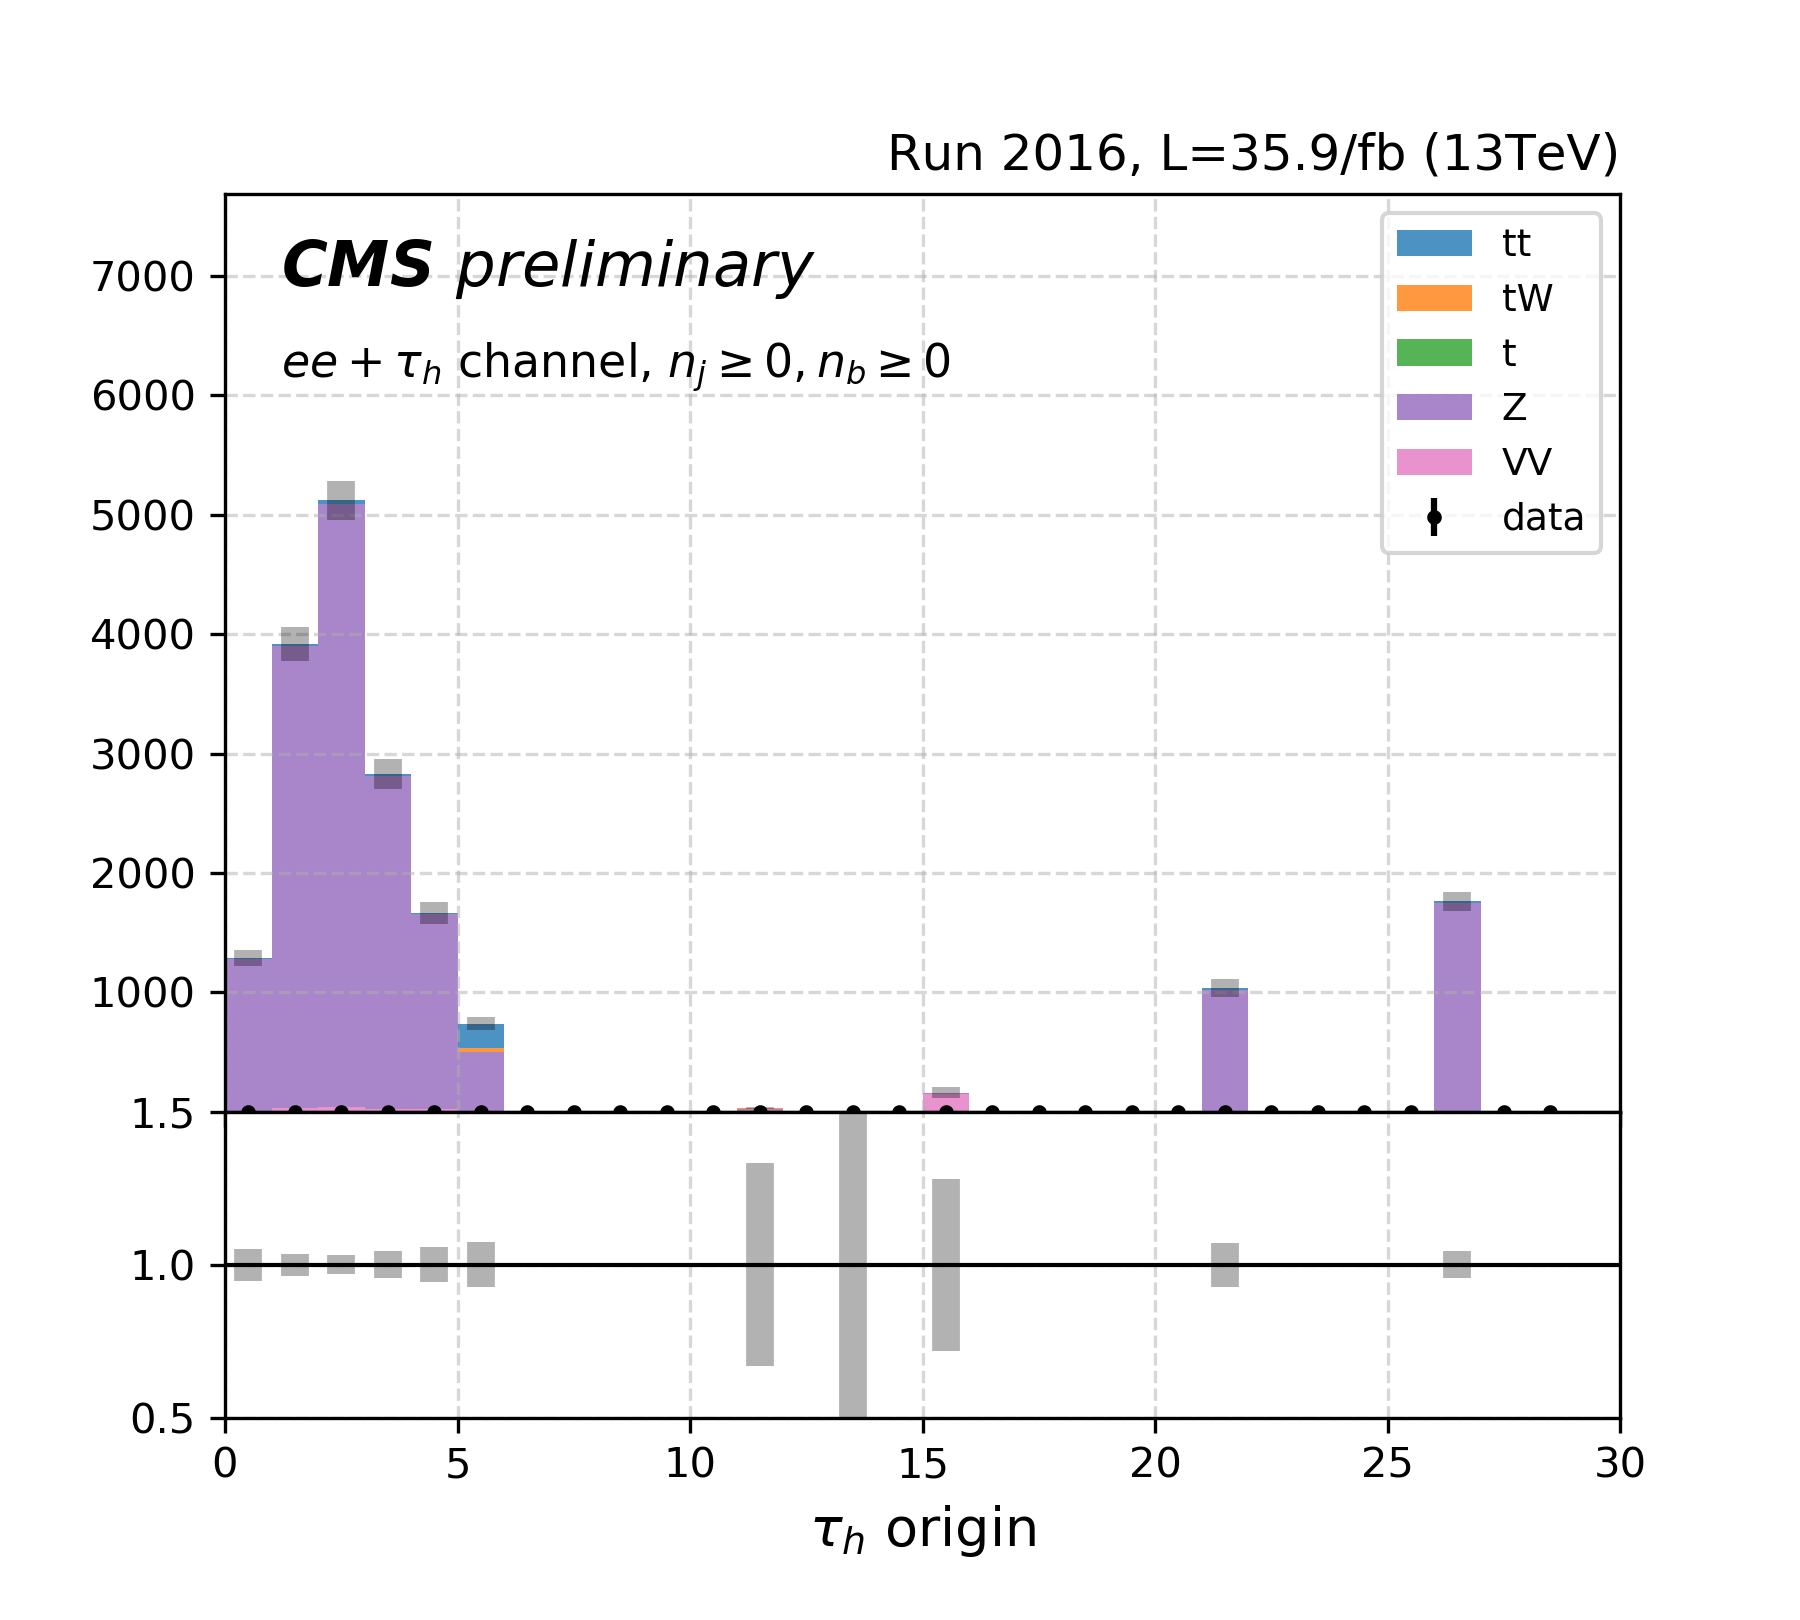
\includegraphics[width=0.4\textwidth]{chapters/Appendix/sectionJetToTauh/figures/eetau_tauGenFlavor_pickles_lltauVTight.png}
    \caption{Distributions of $m_{ee}$, $\tau pT$ and gen-level $\tau_h$ origin in the $ee+\tau$ channel. The left and right column shows the Tight and VTight $\tau_h$ WP respectively.}
    \label{fig:appendix:fakeTauId:eetau}
\end{figure}


\begin{figure}
    \centering
    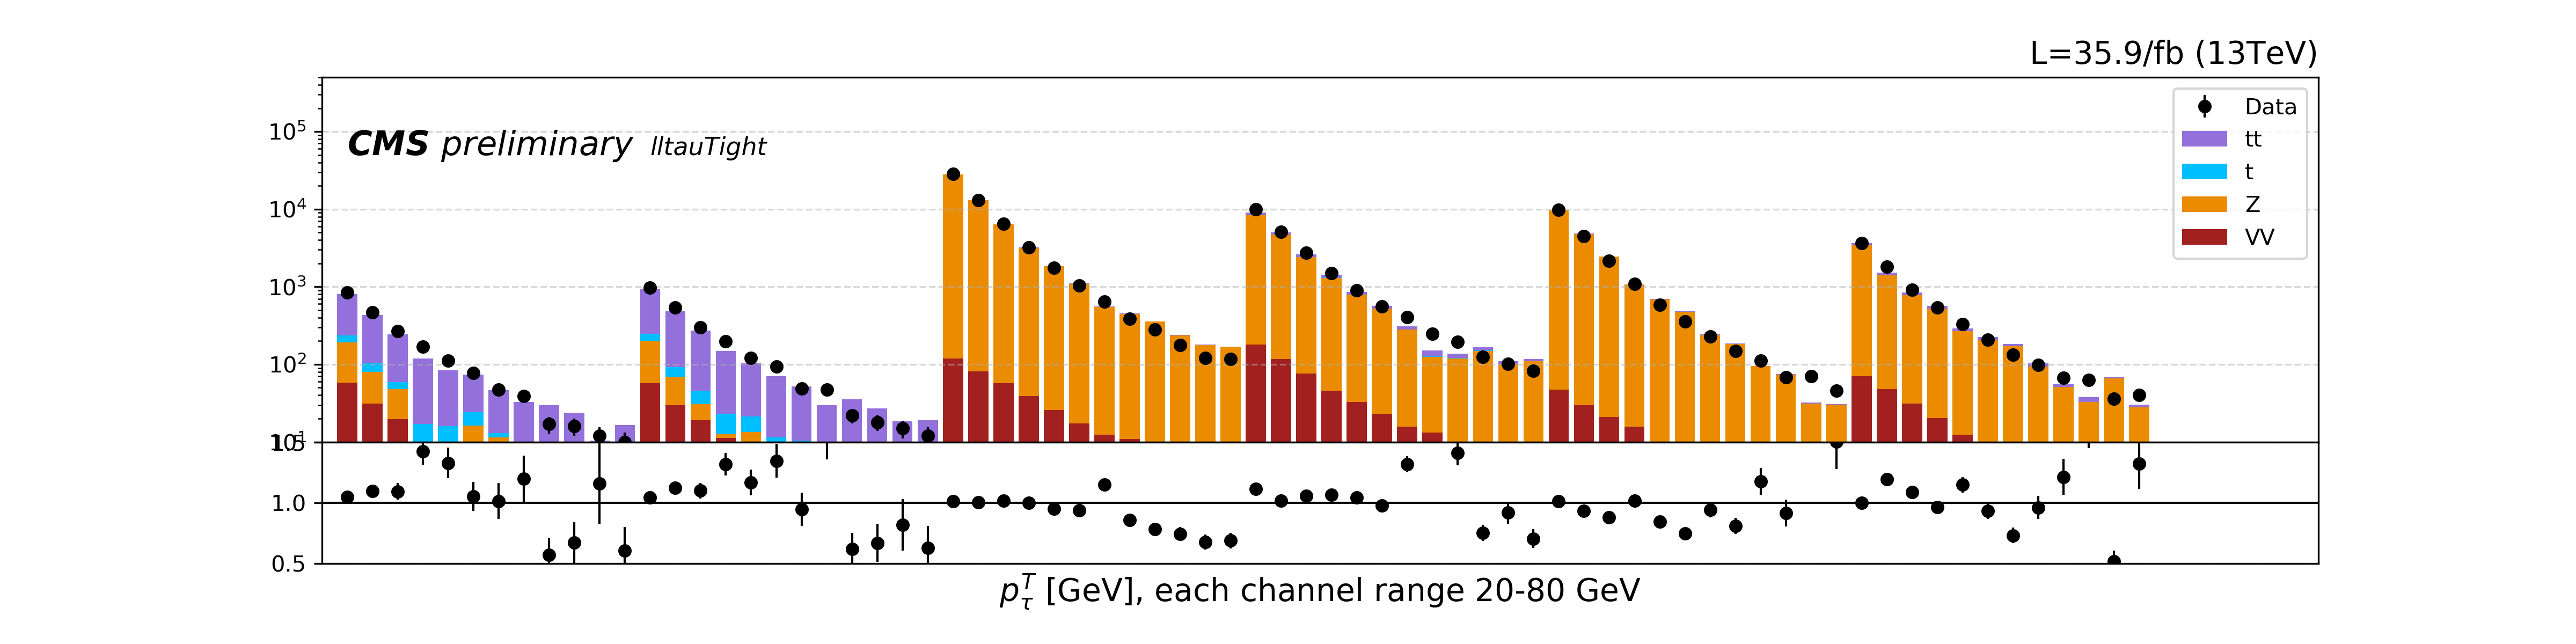
\includegraphics[width=0.99\textwidth]{chapters/Appendix/sectionJetToTauh/figures/2020_tauID_prefit_lltauTight.png}
    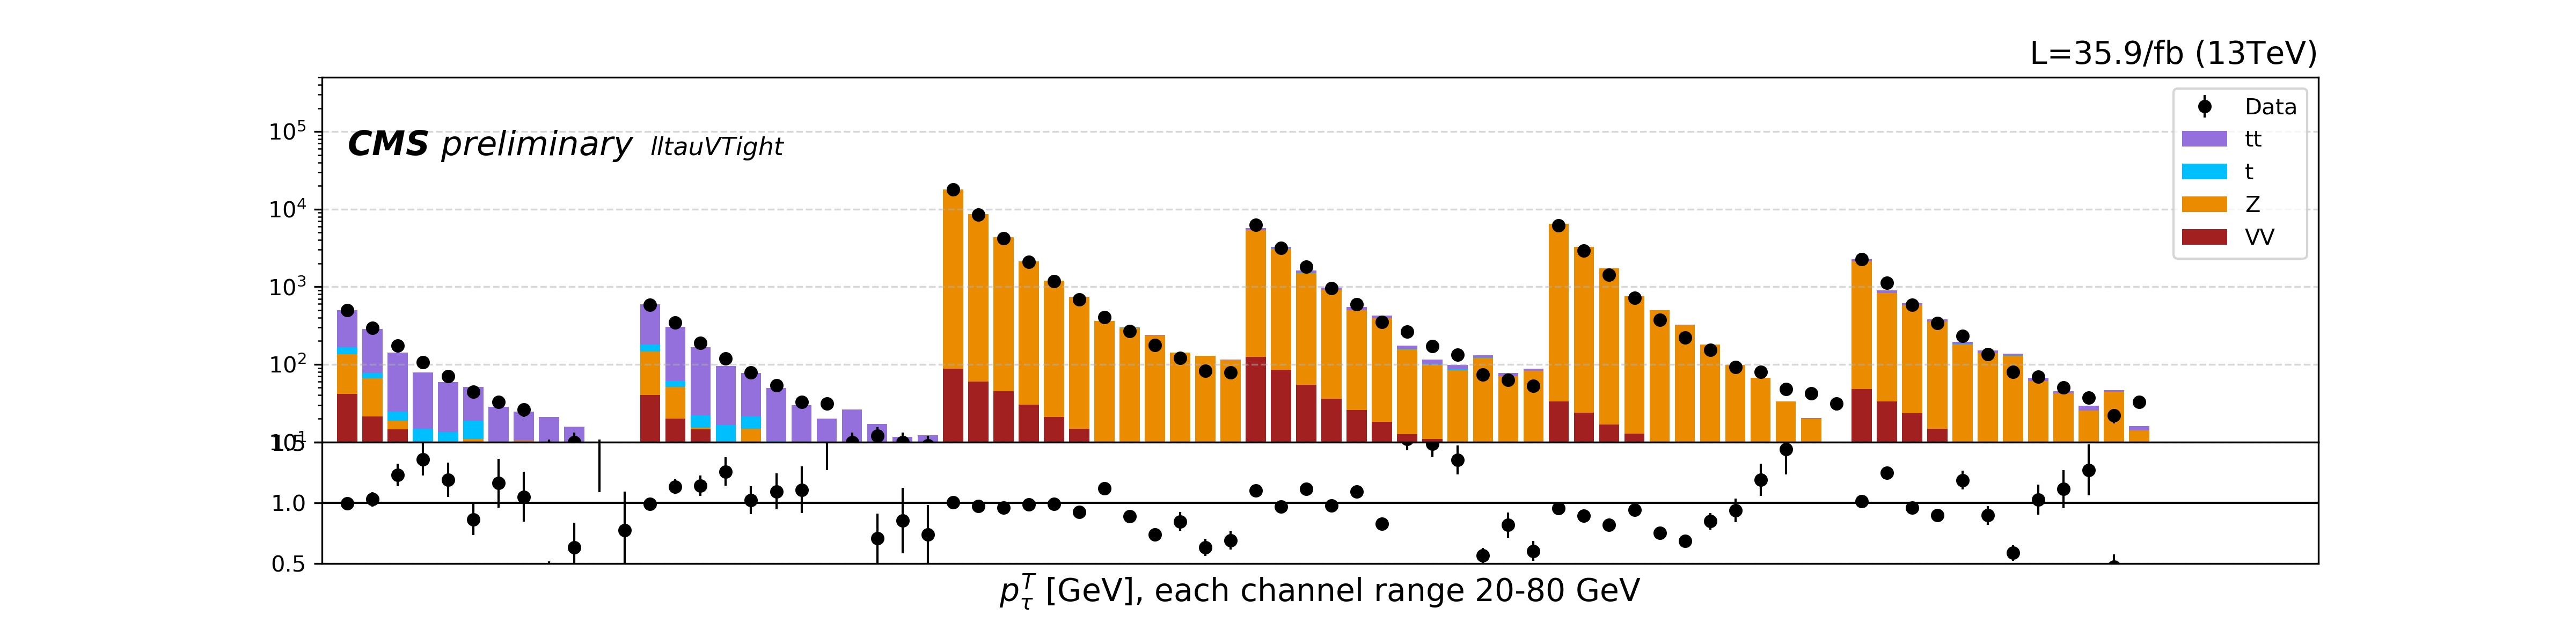
\includegraphics[width=0.99\textwidth]{chapters/Appendix/sectionJetToTauh/figures/2020_tauID_prefit_lltauVTight.png}
    \caption{Prefit distributions}
    \label{fig:appendix:fakeTauId:prefit}
\end{figure}

\begin{figure}
    \centering
    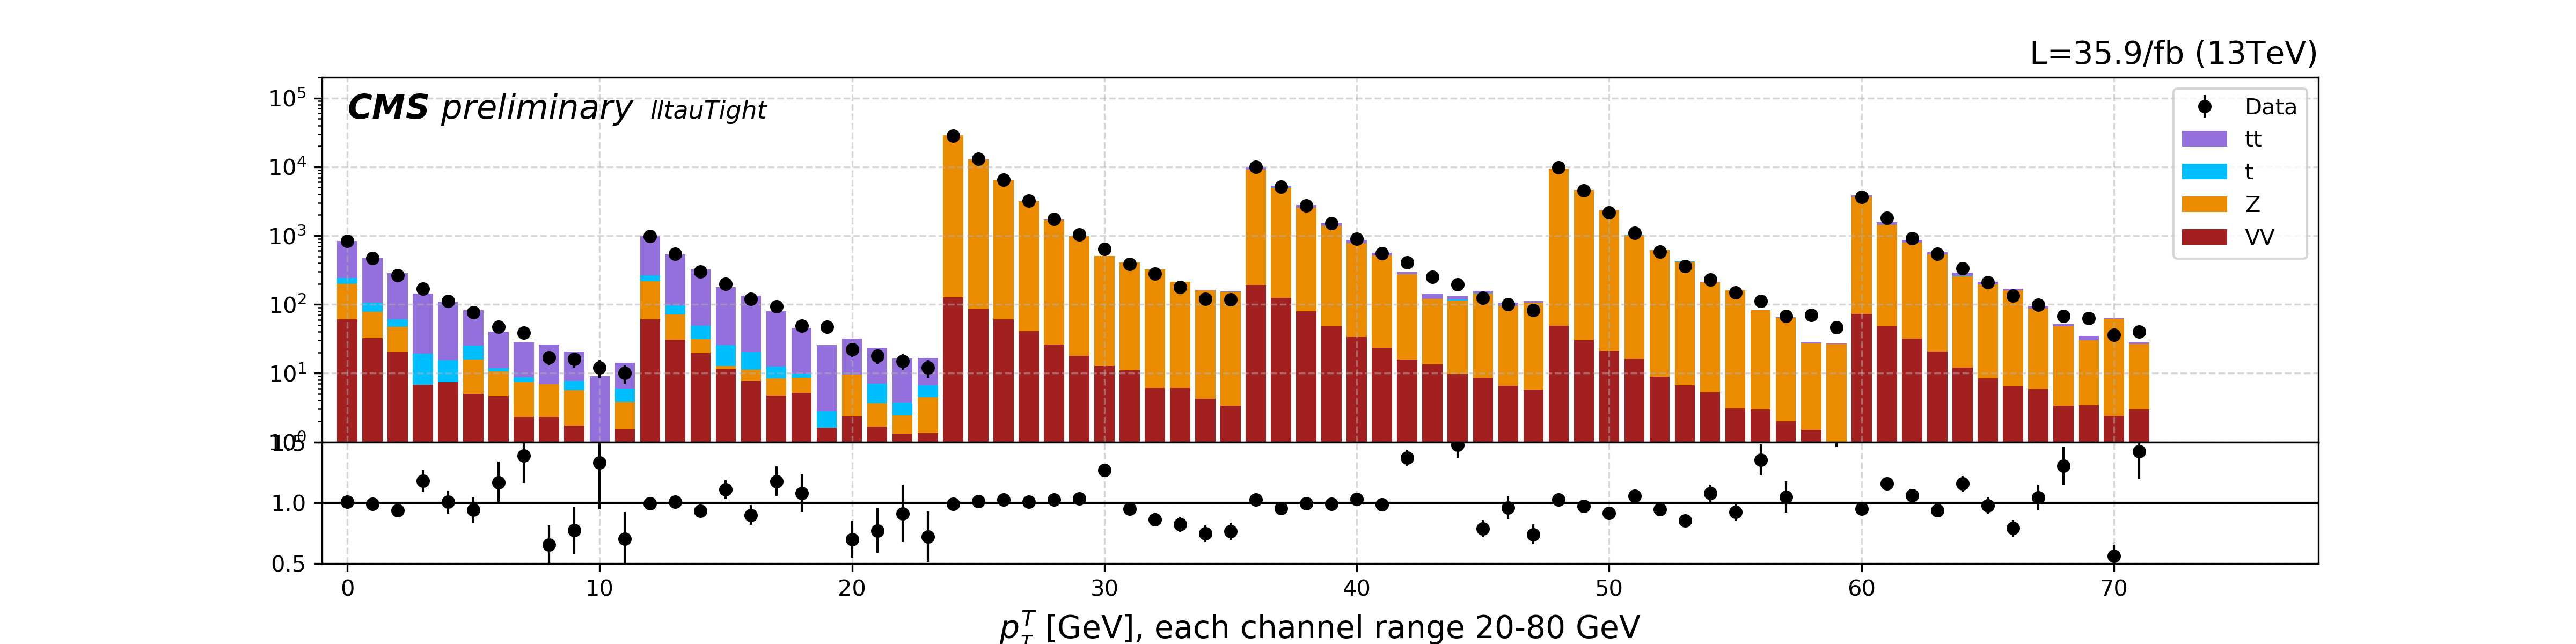
\includegraphics[width=0.99\textwidth]{chapters/Appendix/sectionJetToTauh/figures/2020_tauID_postfit_lltauTight.png}
    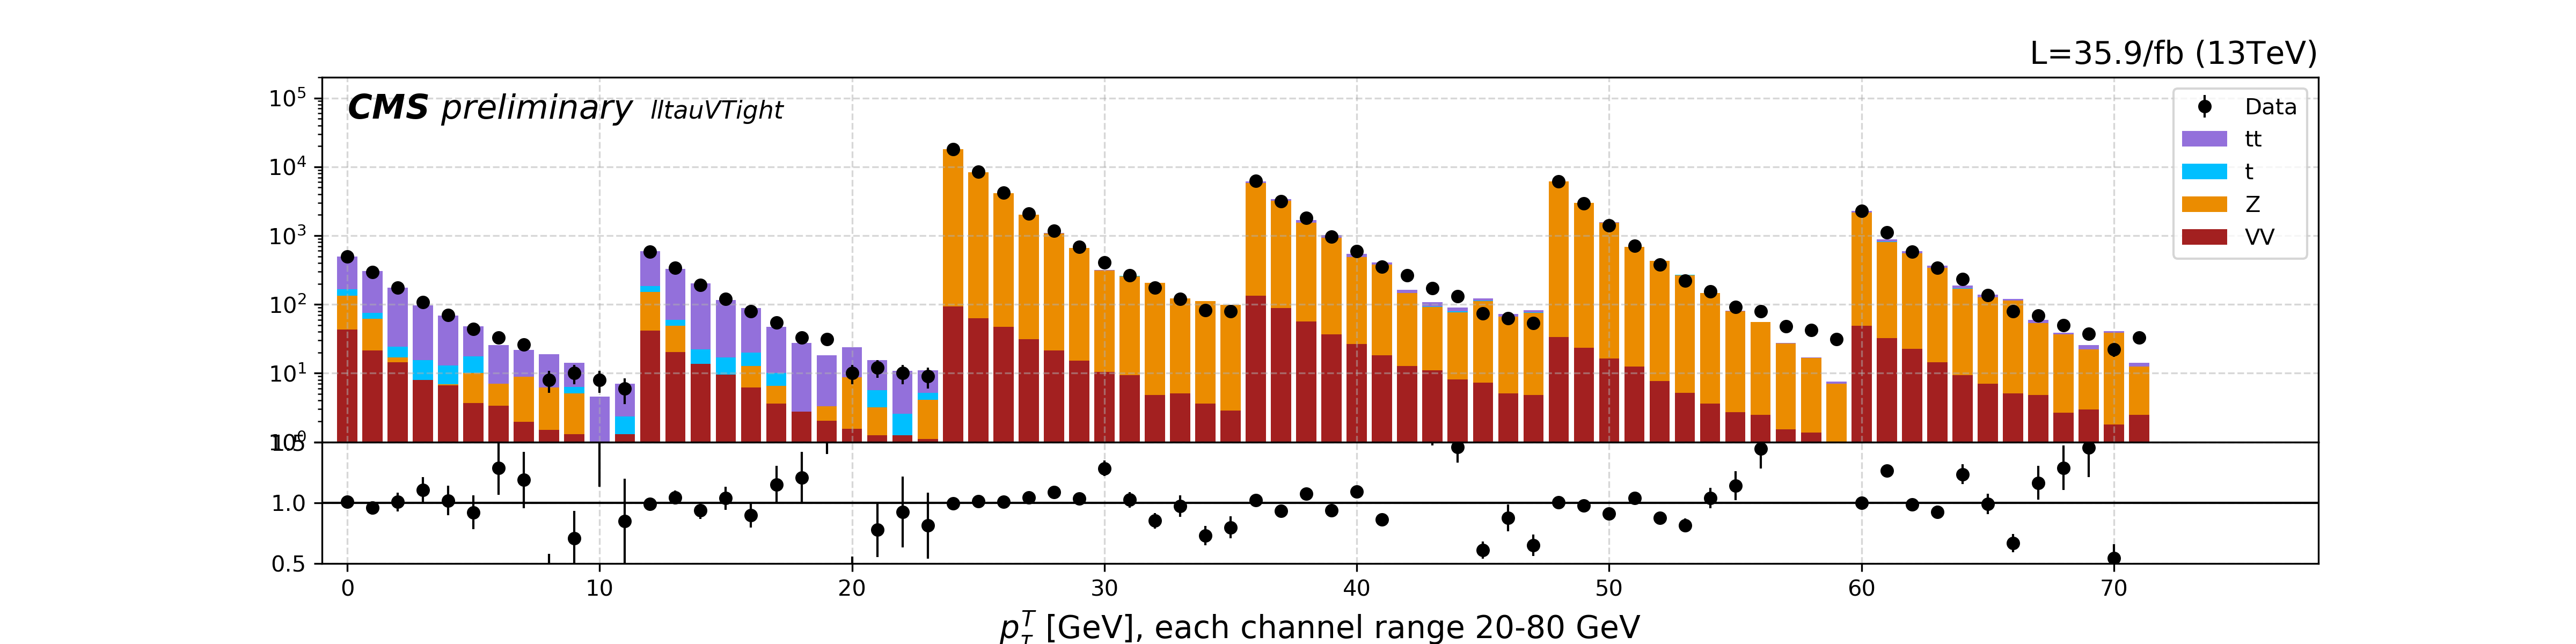
\includegraphics[width=0.99\textwidth]{chapters/Appendix/sectionJetToTauh/figures/2020_tauID_postfit_lltauVTight.png}
    \caption{Post distributions}
    \label{fig:appendix:fakeTauId:postfit}
\end{figure}


\begin{figure}
    \centering
    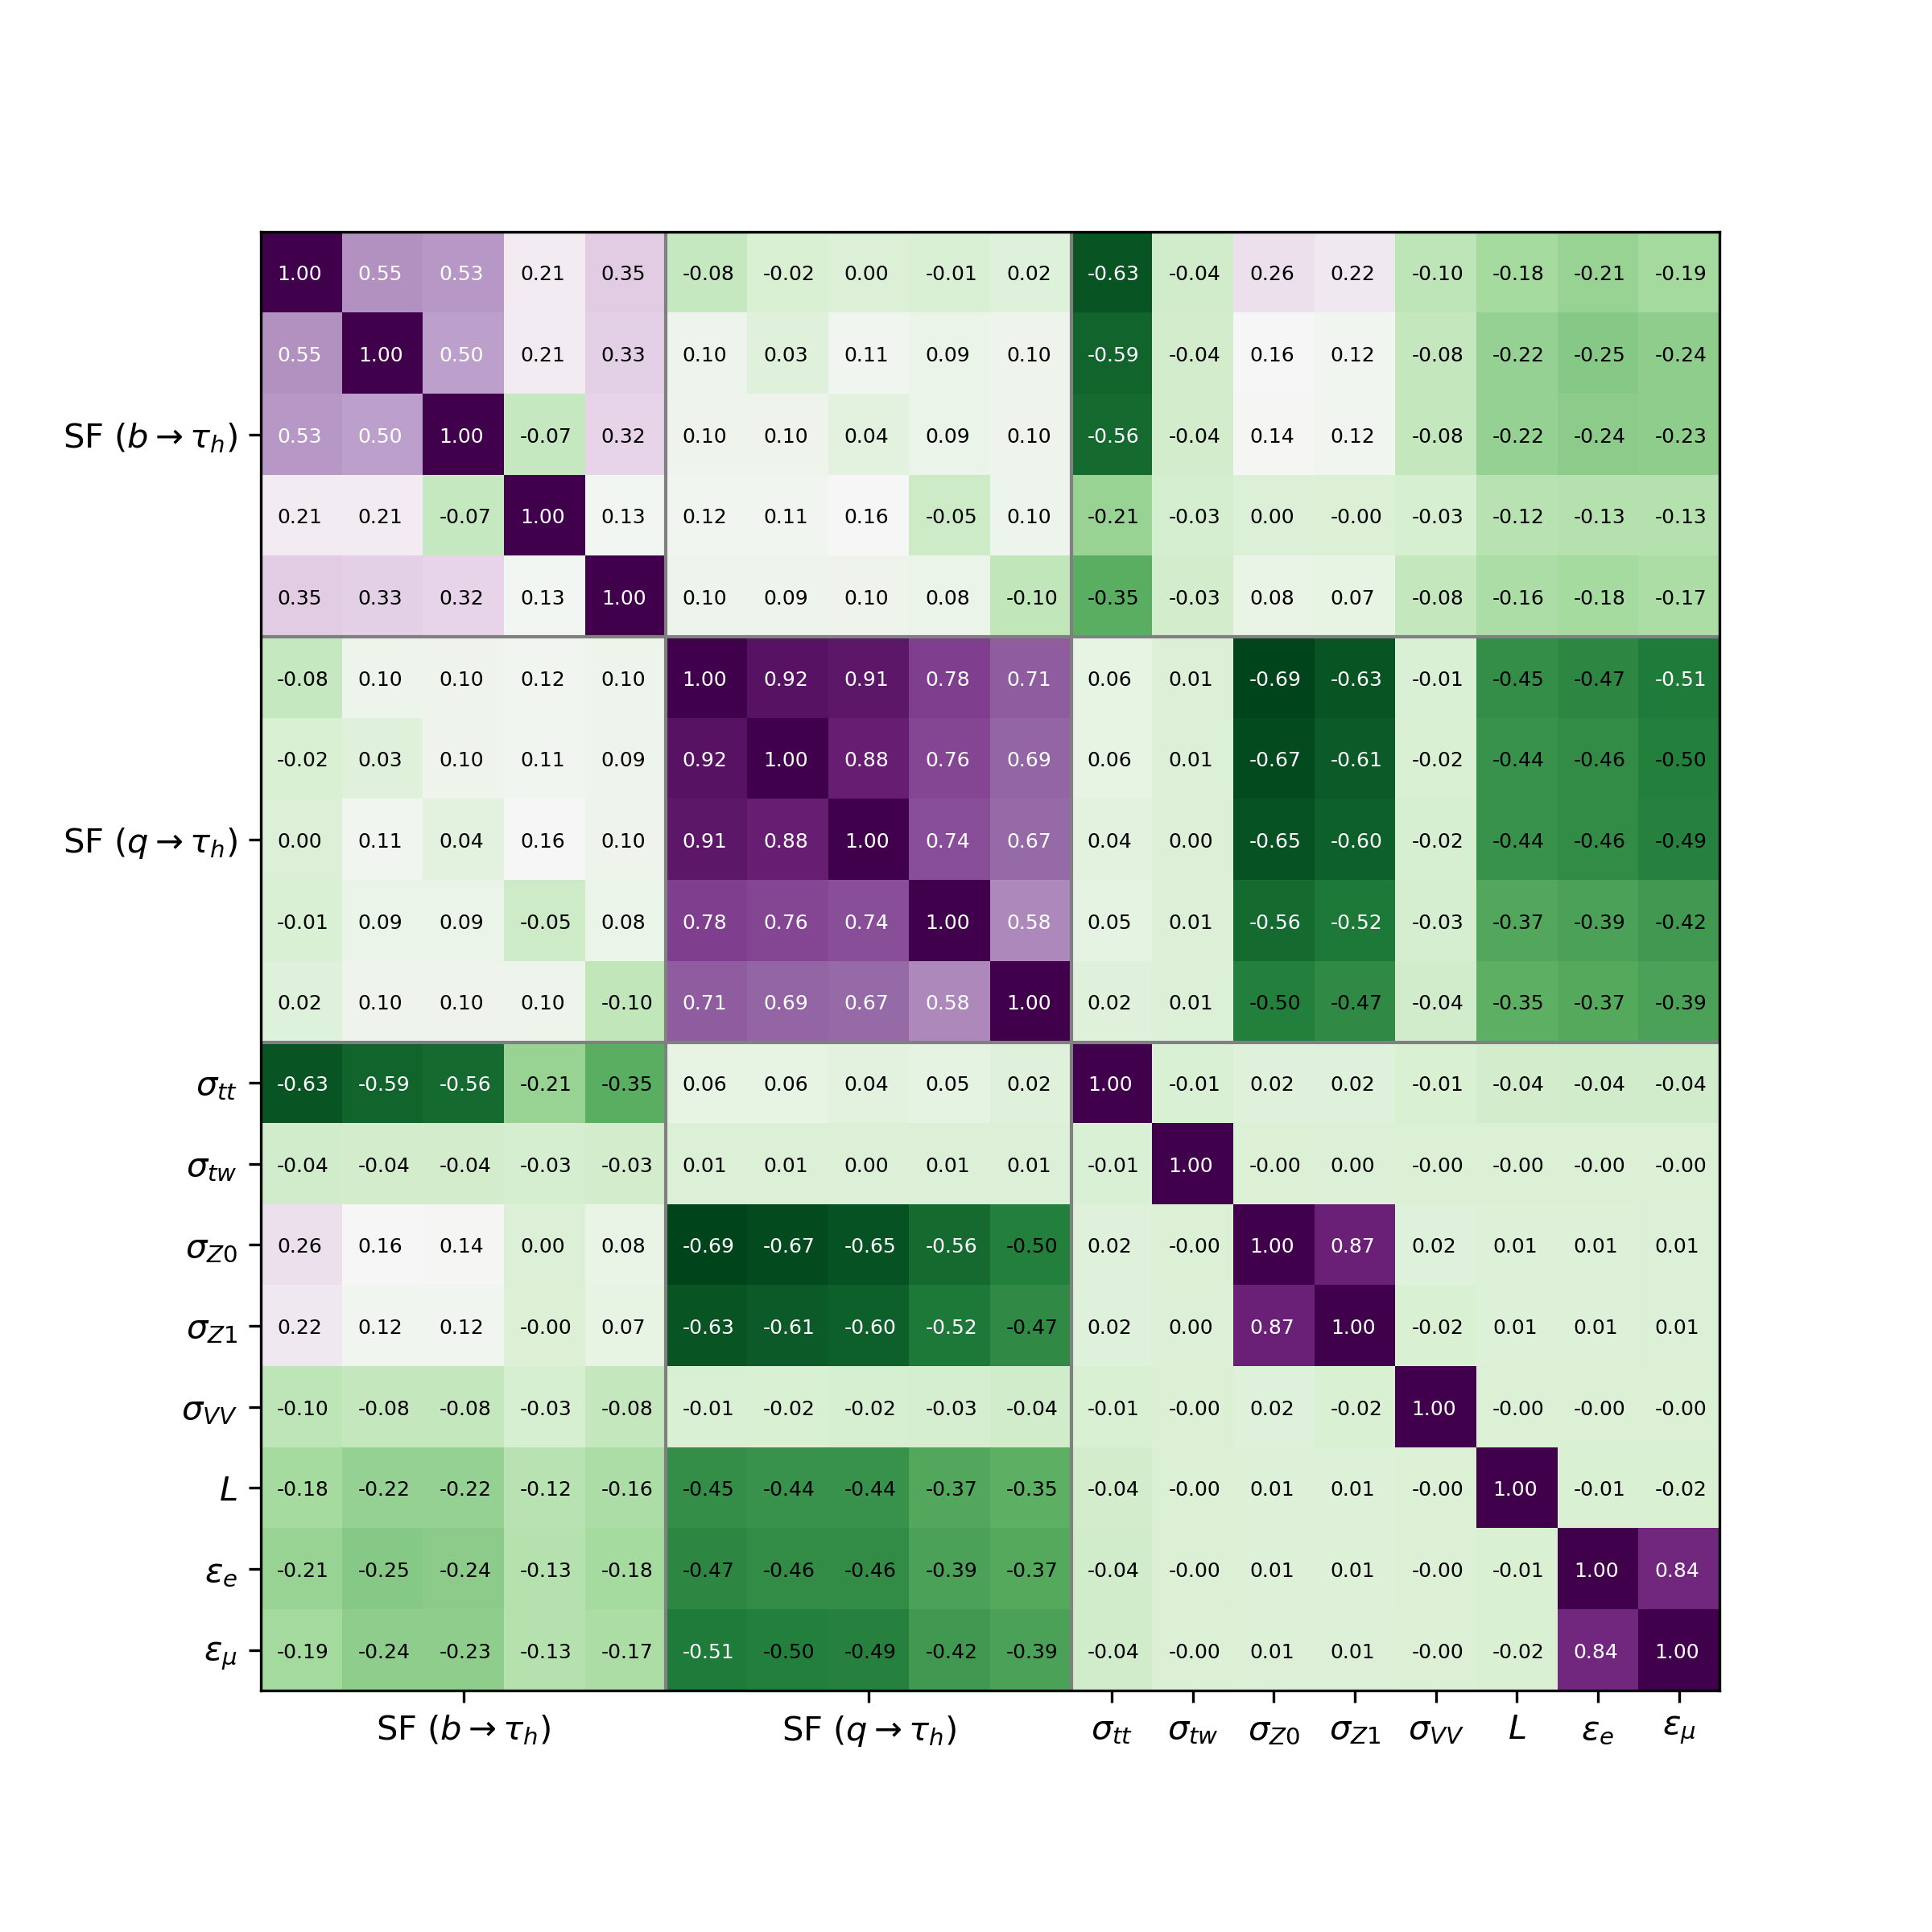
\includegraphics[width=0.49\textwidth]{chapters/Appendix/sectionJetToTauh/figures/corr2_lltauTight_splitJetFlavor.png}
    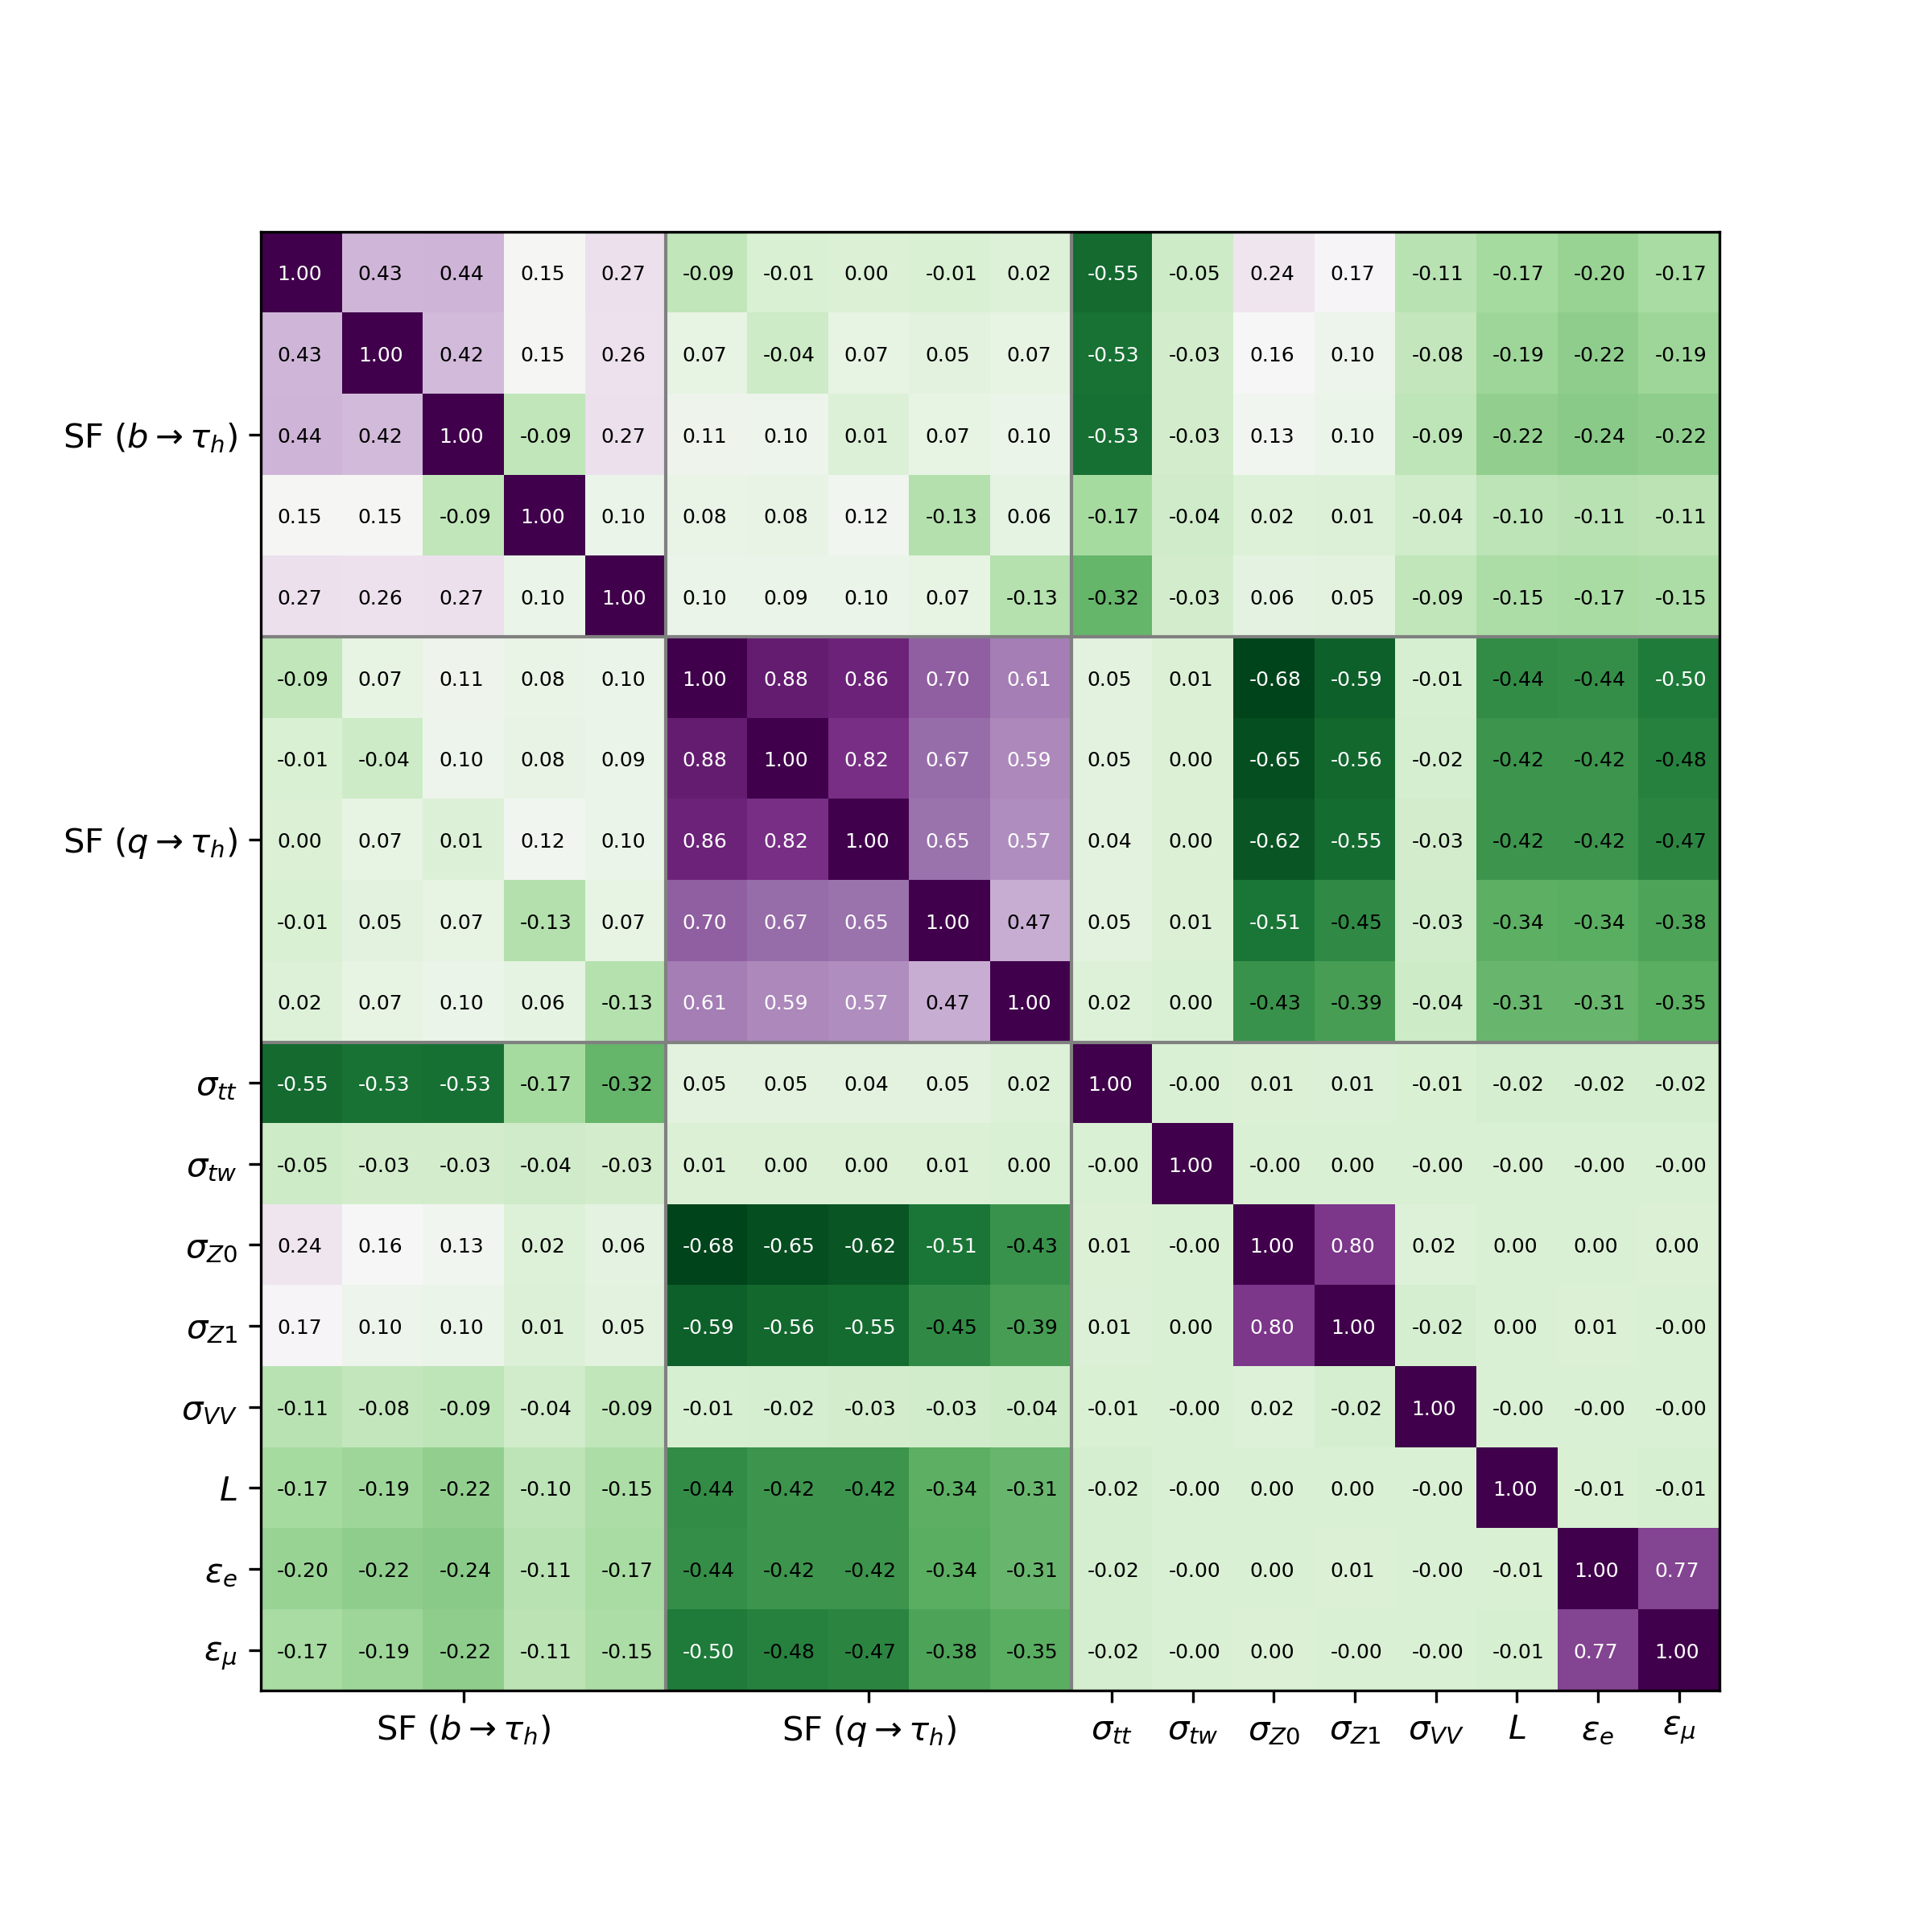
\includegraphics[width=0.49\textwidth]{chapters/Appendix/sectionJetToTauh/figures/corr2_lltauVTight_splitJetFlavor.png}
    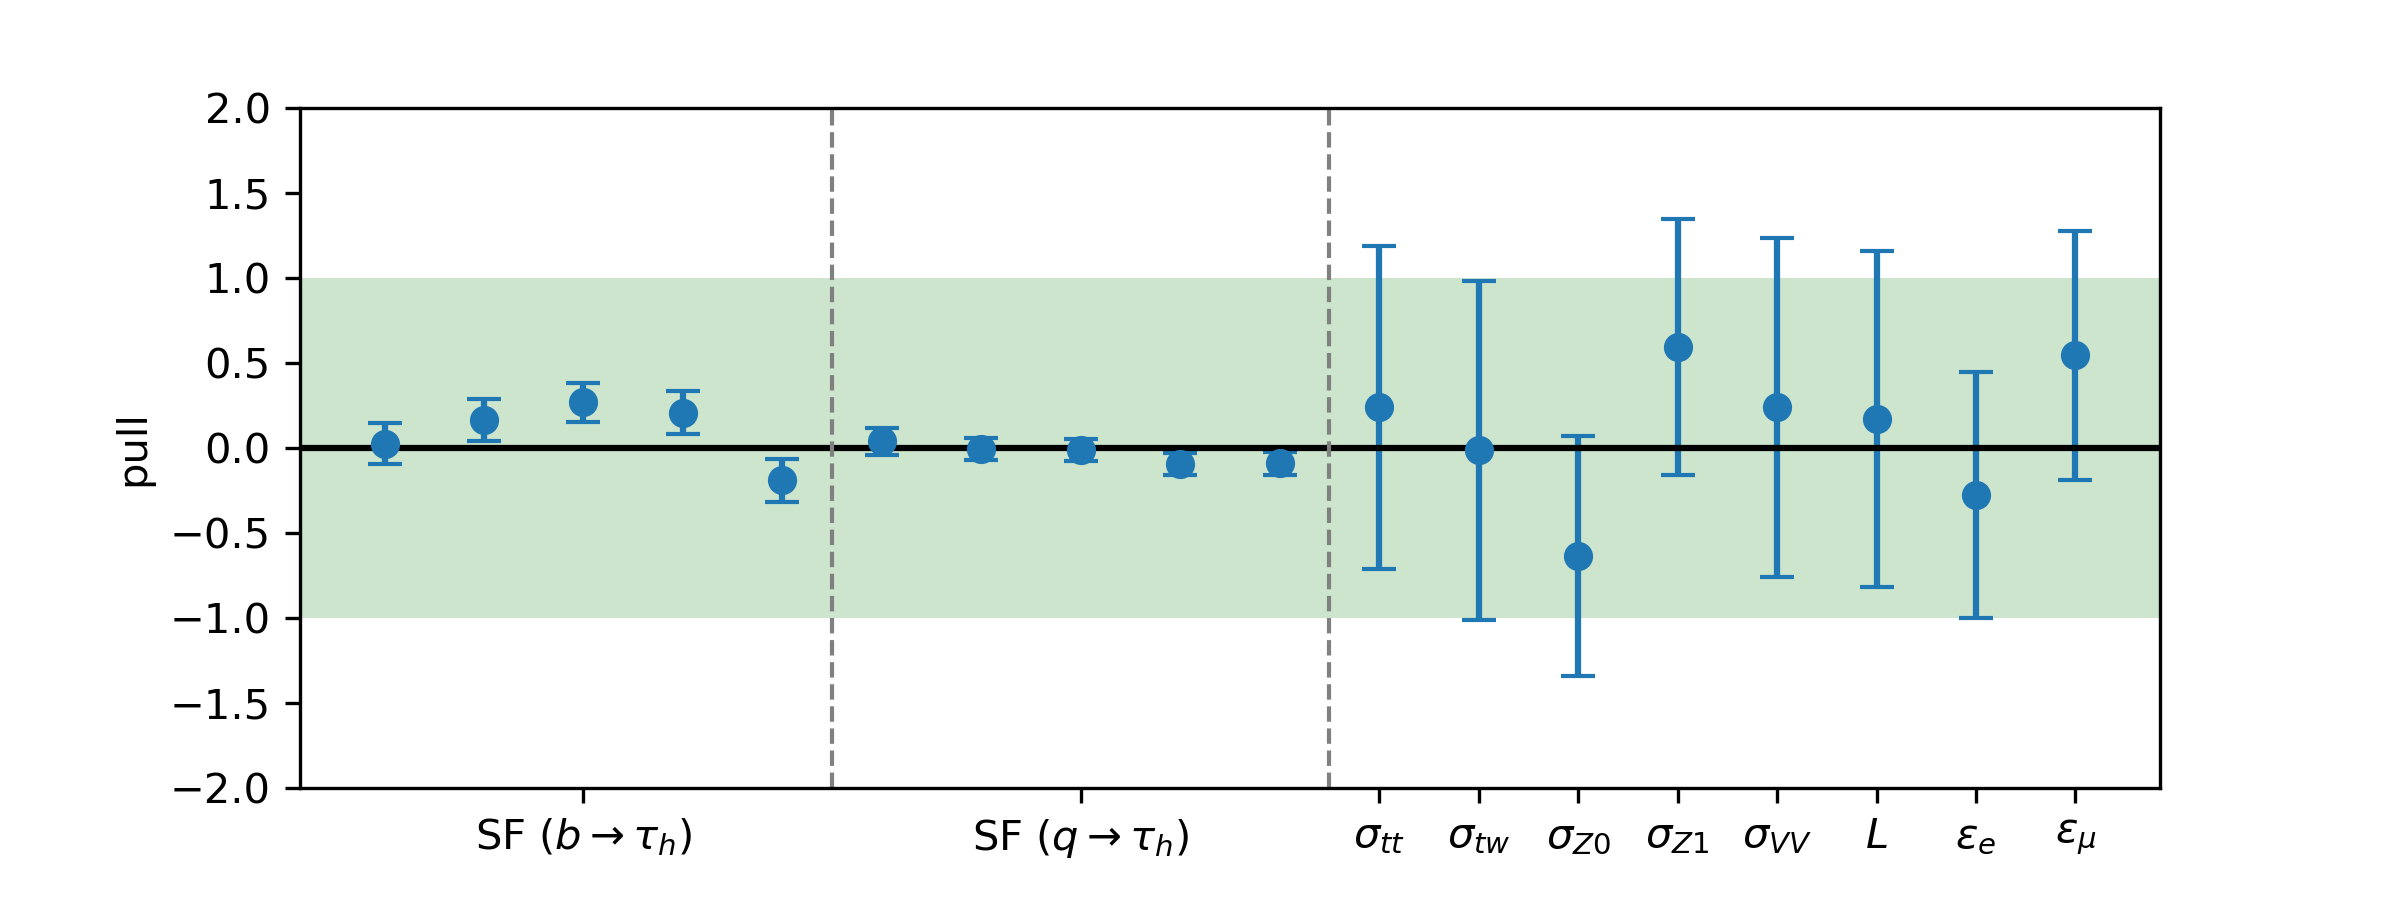
\includegraphics[width=0.49\textwidth]{chapters/Appendix/sectionJetToTauh/figures/pull2_lltauTight_splitJetFlavor.png}
    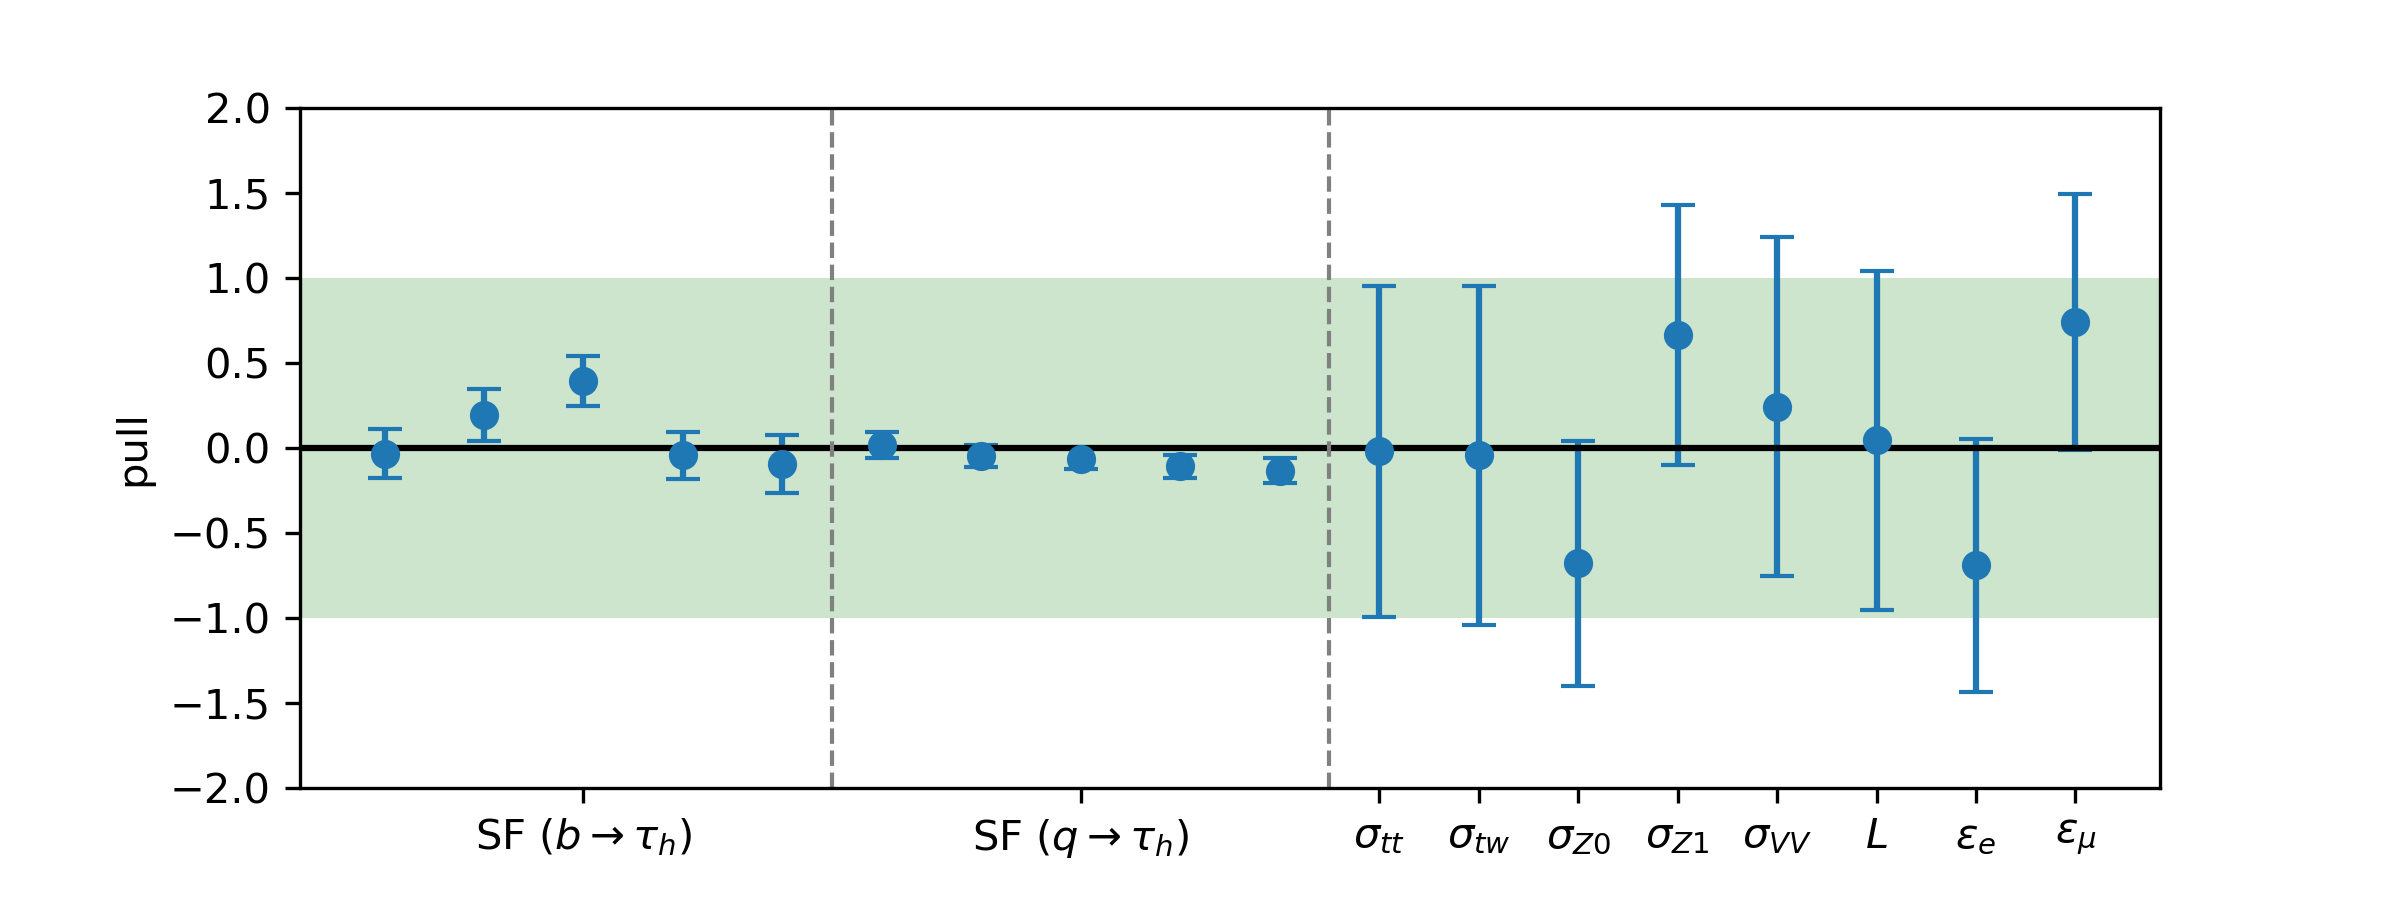
\includegraphics[width=0.49\textwidth]{chapters/Appendix/sectionJetToTauh/figures/pull2_lltauVTight_splitJetFlavor.png}
    \caption{The correlation coefficients and pull of fitting parameters}
    \label{fig:appendix:fakeTauId:fitparam}
\end{figure}

\begin{figure}
    \centering
    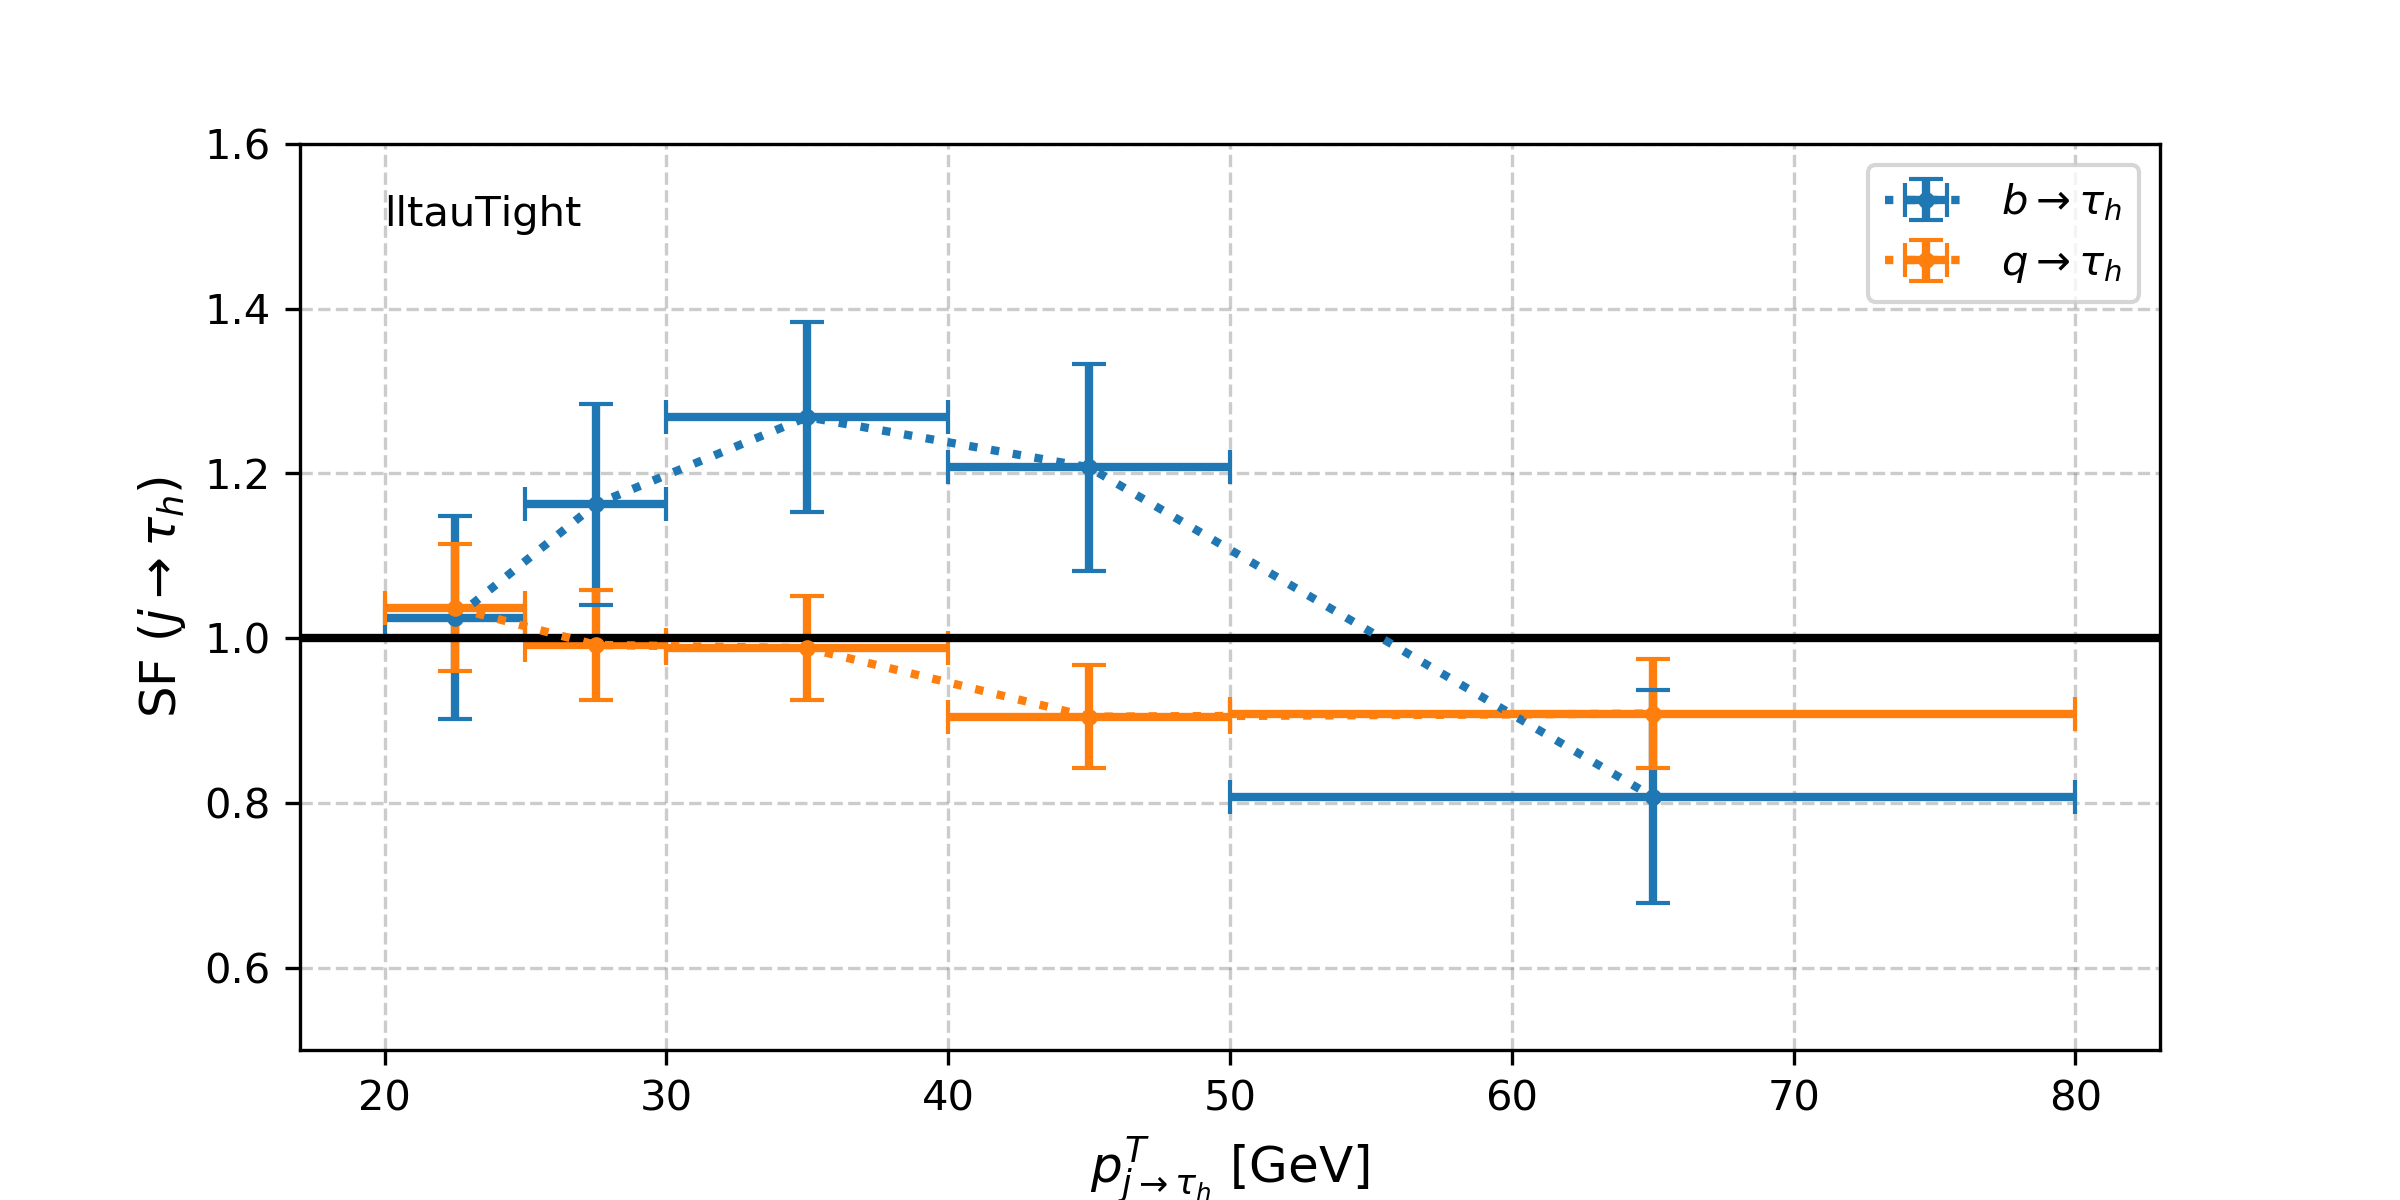
\includegraphics[width=0.49\textwidth]{chapters/Appendix/sectionJetToTauh/figures/fit2_ptflavor2_lltauTight.png}
    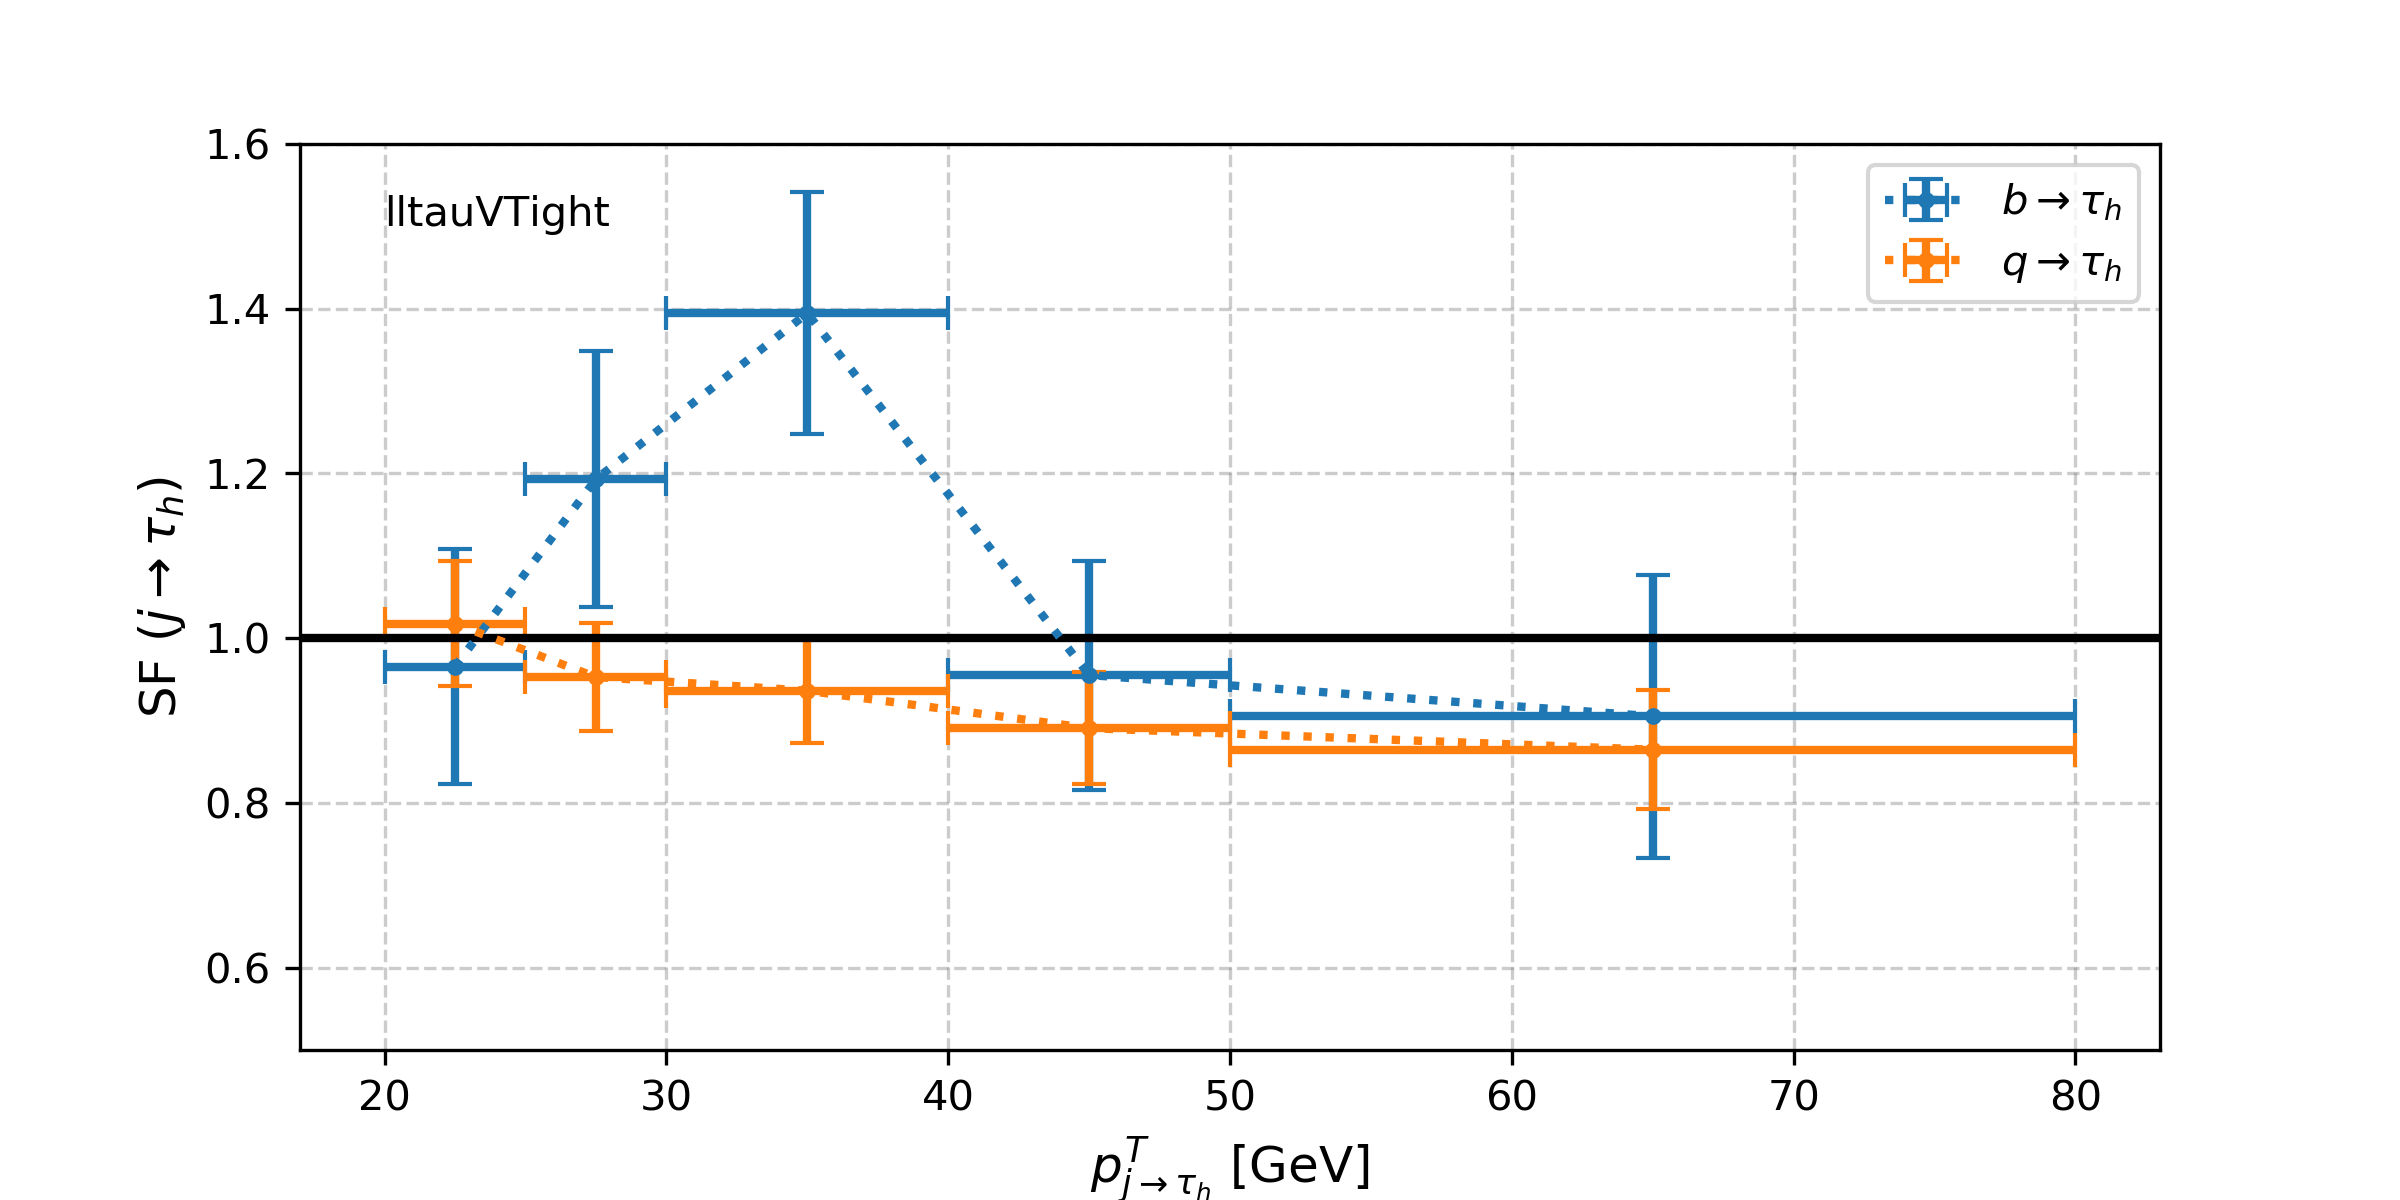
\includegraphics[width=0.49\textwidth]{chapters/Appendix/sectionJetToTauh/figures/fit2_ptflavor2_lltauVTight.png}
    \caption{SF}
    \label{fig:appendix:fakeTauId:fit}
\end{figure}

\begin{table}[h]
    \setlength{\tabcolsep}{6pt} % Default value: 6pt
    \renewcommand{\arraystretch}{1.5} % Default value: 1
    \begin{tabular}{c|ccccc}
    \hline
    $p^T_{\tau_h}$ [GeV]  & 20-25         & 25-30         & 30-40         & 40-50         & 50-80         \\
    \hline
    $SF(b\to Tight \cdot \tau_h)$  & $1.02\pm0.12$ & $1.16\pm0.12$ & $1.27\pm0.11$ & $1.21\pm0.13$ & $0.81\pm0.13$ \\
    $SF(q\to Tight \cdot \tau_h)$  & $1.04\pm0.08$ & $0.99\pm0.07$ & $0.99\pm0.06$ & $0.90\pm0.06$ & $0.91\pm0.07$ \\
    \hline
    $SF(b\to VTight \cdot\tau_h)$ & $0.97\pm0.14$ & $1.19\pm0.16$ & $1.39\pm0.15$ & $0.96\pm0.14$ & $0.91\pm0.17$ \\
    $SF(q\to VTight \cdot\tau_h)$ & $1.02\pm0.08$ & $0.95\pm0.07$ & $0.94\pm0.06$ & $0.89\pm0.07$ & $0.86\pm0.07$ \\
    \hline
    \end{tabular}
    \caption{ $SF (j\to \tau_h)$ for Tight and VTight tau MVA}
\end{table}

\section{Reweight of $B(\tau \to  \rm{hadrons})$}

The MC events with $\tau_h$ in the $e\tau$ and $\mu \tau$ channel is essential to the sensitivity of the
$Br(W\to\tau)$ measurement. However, the tau's hadronic decay branching fraction $B(\tau \to  \rm{hadrons})$
in the MC simulation are different from the experimental world average in the PDG.
The $\tau_h$ selection efficiency could be impacted by such difference because various tau's hadronic 
decay mode have different efficiencies in the CMS $\tau_h$ reconstruction with SPH algorithm.

Thus it is necessary to reweight the MC events to correct the deviation of tau's decay in the simulation
with respect to the PDG values. For the values in the \PYTHIA simulation assumption and the PDG world average,
tau's hadronic decay branching fractions are listed in table~\ref{tab:tauhReweighting}. The difference between 
values in \PYTHIA8 and PDG is about $0.5\%$. The ratios of PDG and
\PYTHIA values are also included, which are the event weights applied for the $\tau \to h$ reweighting.

    
    
\begin{table}[ht]
  \centering
  \setlength{\tabcolsep}{1 em}
  \renewcommand{\arraystretch}{1.5}
  \caption{ The values of $B(\tau \to  \rm{hadrons})$ in PYTHIA8 and in PDG.}
  \begin{tabular}{l|c|c|c}
  \hline
                              & PDG        & \PYTHIA   & PDG / \PYTHIA \\
  \hline
  $Br(\tau\to \pi^\pm)$       & 0.1082(5)  & 0.1076825 & 1.00481       \\
  $Br(\tau\to \pi^\pm+ \pi^0)$& 0.2549(9)  & 0.2537447 & 1.00455       \\
  $Br(\tau\to \pi^\pm+2\pi^0)$& 0.0926(10) & 0.0924697 & 1.00141       \\
  $Br(\tau\to3\pi^\pm)$       & 0.0931(5)  & 0.0925691 & 1.00574       \\
  $Br(\tau\to3\pi^\pm+ \pi^0)$& 0.0462(5)  & 0.0459365 & 1.00574       \\
  \hline
  \end{tabular}
  \label{tab:tauhReweighting}
\end{table}


\begin{figure}
    \centering
    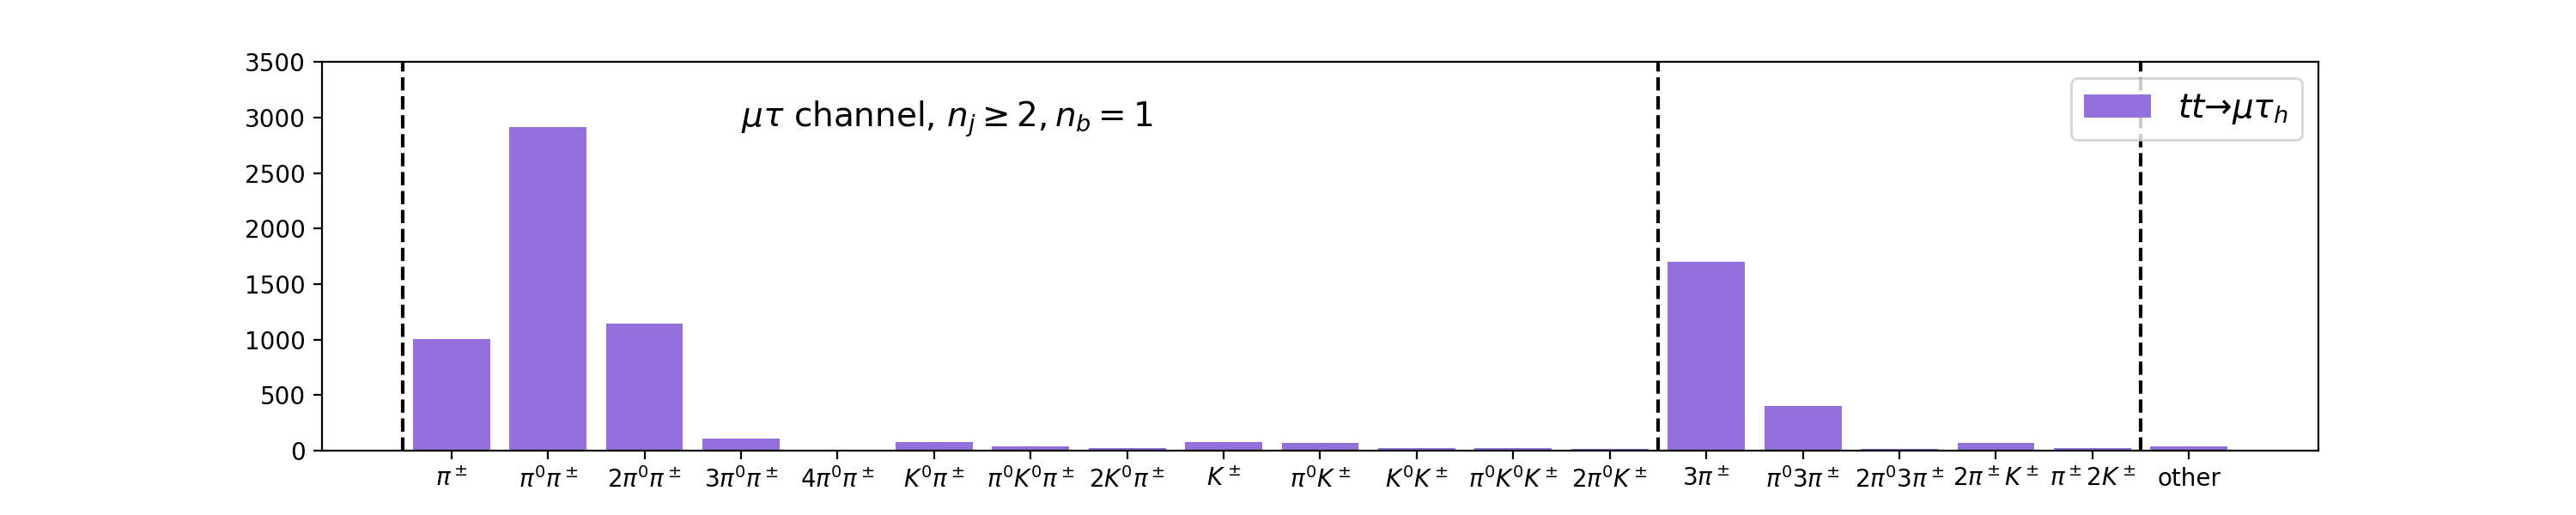
\includegraphics[width=0.99\textwidth]{chapters/Appendix/sectionTauBr/figures/tauhDecay_mutau.png}
    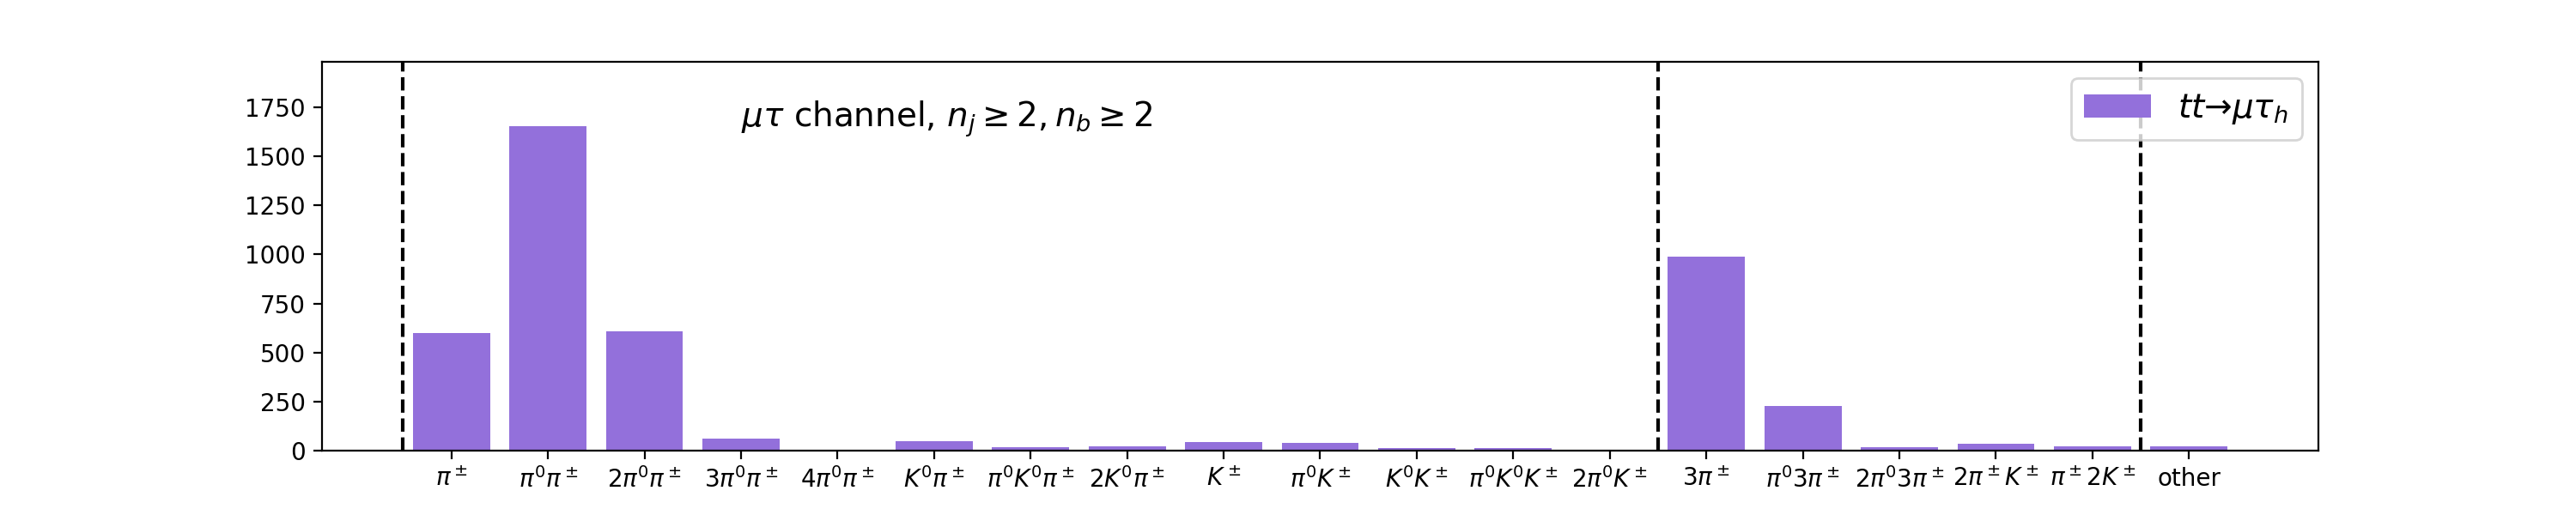
\includegraphics[width=0.99\textwidth]{chapters/Appendix/sectionTauBr/figures/tauhDecay_mutau2.png}
    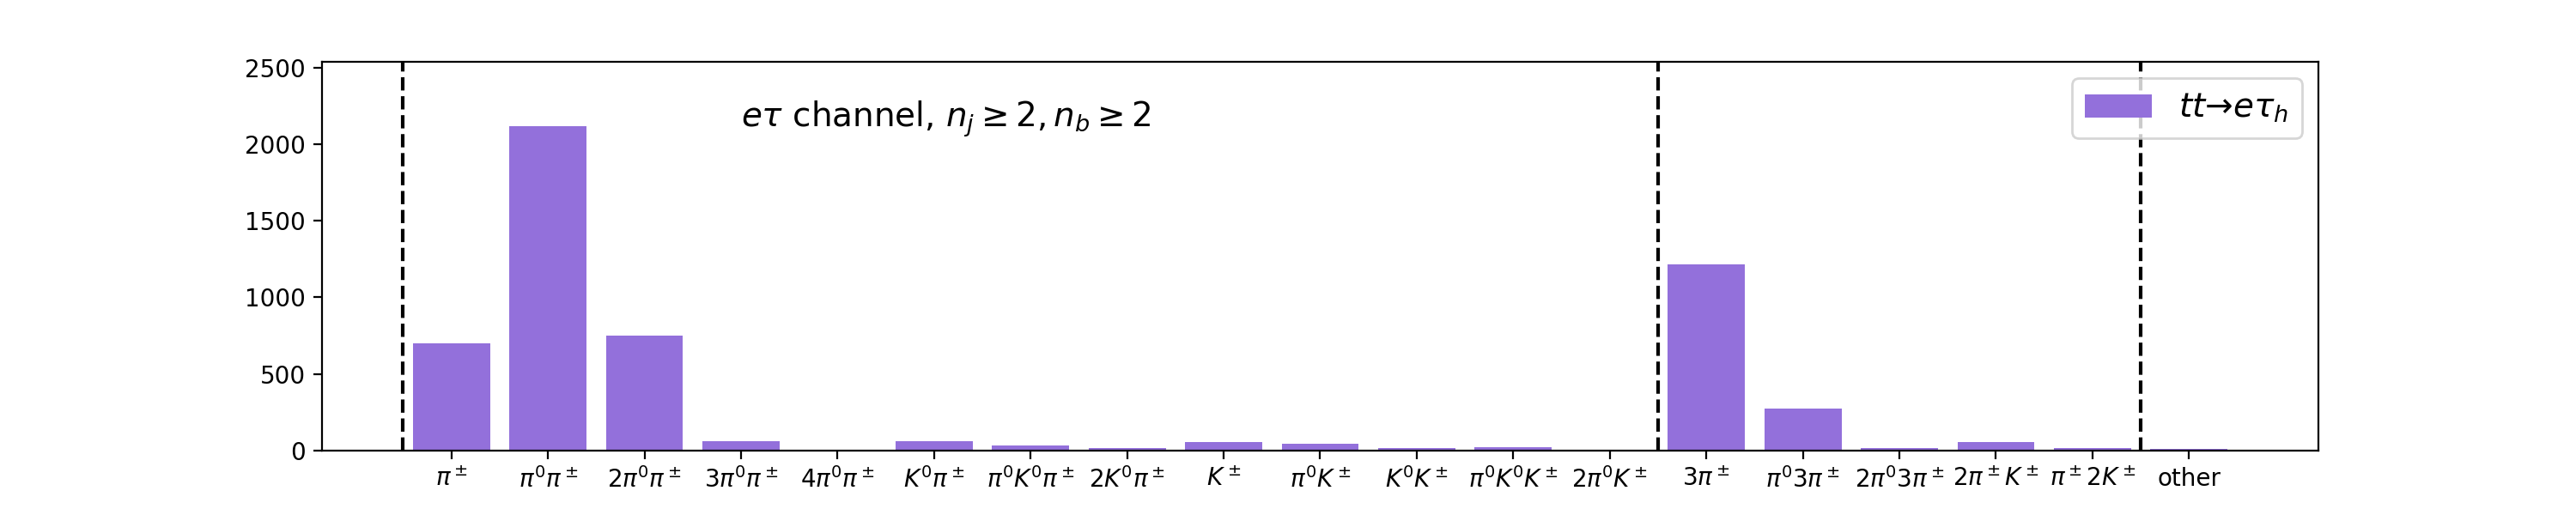
\includegraphics[width=0.99\textwidth]{chapters/Appendix/sectionTauBr/figures/tauhDecay_etau.png}
    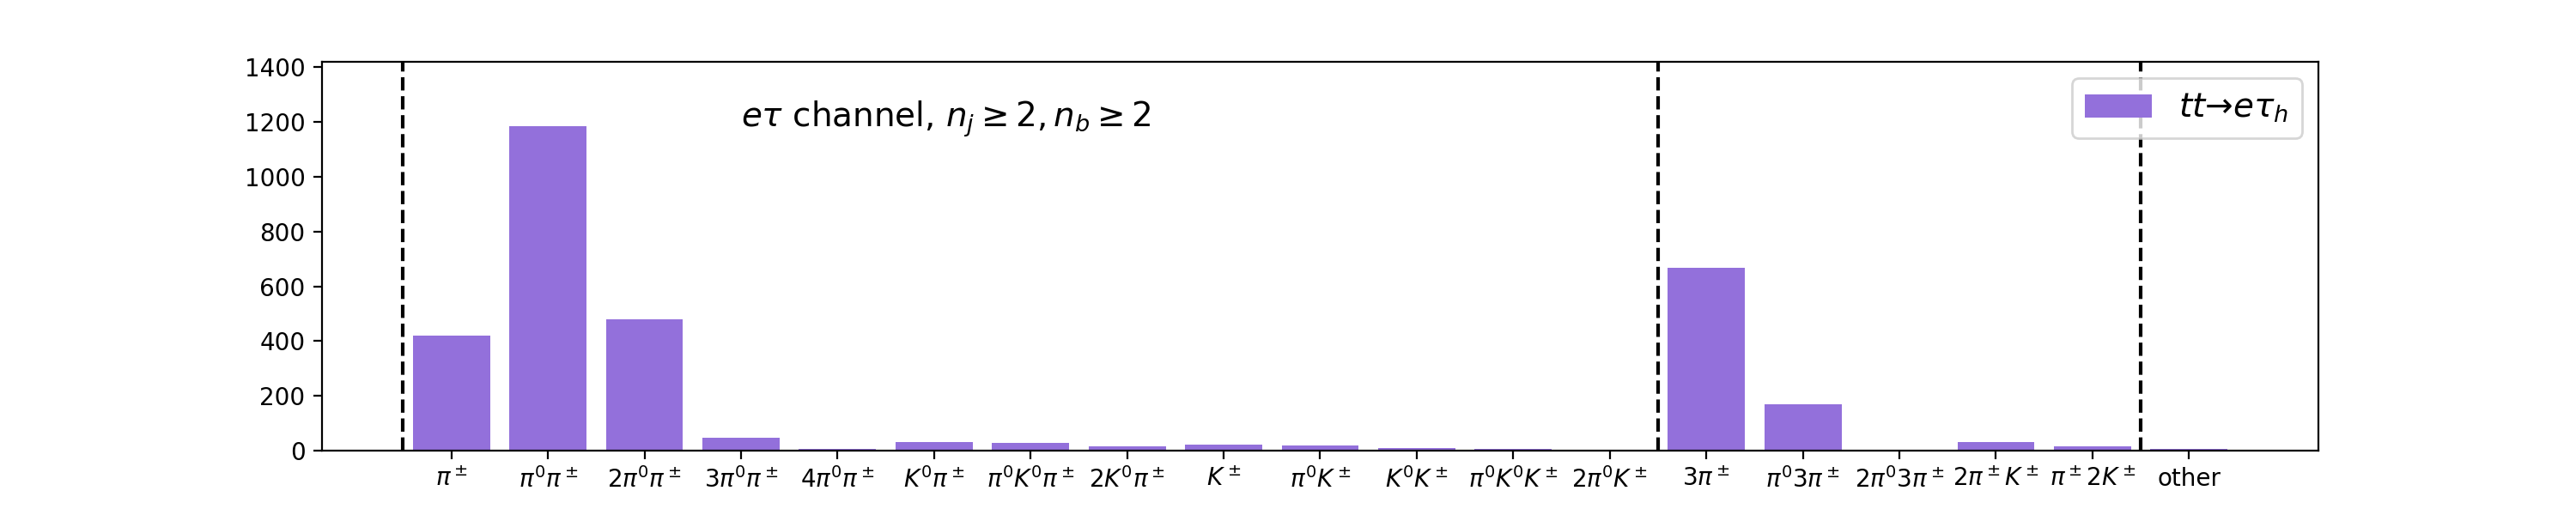
\includegraphics[width=0.99\textwidth]{chapters/Appendix/sectionTauBr/figures/tauhDecay_etau2.png}
    \caption{The gen-level daughter mesons from hadronicly decaying taus in the $tt\to \mu \tau_h, e \tau_h$ events passing $\mu \tau$ and $e \tau$ selection.}
    \label{fig:appendix:reweightTauhBr:tauhBr}
\end{figure}


In MC events, the gen-level daughter mesons from hadronicly decaying taus are saved. 
The $\tau_h$'s daughter mesons in the $tt\to \mu \tau_h, e \tau_h$ events 
passing $\mu \tau$ and $e \tau$ selection are shown
in Fig~\ref{fig:appendix:reweightTauhBr:tauhBr}
The leading contributions to the reconstructed $\tau_h$ are 
$\tau\to \pi^\pm+\pi^0 $, $\tau\to 3\pi^\pm$, $\tau\to \pi^\pm+2\pi^0$, $\tau\to
\pi^\pm$, $\tau\to 3\pi^\pm + \pi^0$. 
MC events with taus in those five decay modes are reweighted by 

\begin{equation}
  w = \frac{^{\rm PDG} B(\tau \to  \rm{hadrons}) }{^{\rm PYTHIA} B( \tau \to \rm{hadrons} )}. 
\end{equation} 


\noindent The uncertainties of the weights are from the the PDG uncertainties. 
The systematical uncertainty due to the uncertainties of $B(\tau \to  \rm{hadrons})$ 
reweighting can be estimated. The effect of the $B(\tau \to  \rm{hadrons})$ 
reweighting on the $B(W)$ result is small. The relative
systematics from $B(\tau \to  \rm{hadrons})$ reweighting are about $0.003 - 0.146 \%$, 
shown in table~ \ref{tab:syst_tauhReweighting}.



\begin{table}[p]
  \centering
  \caption{ Relative systematic uncertainty ($\%$) due to $B(\tau \to  \rm{hadrons})$ reweighting.}
  \setlength{\tabcolsep}{0.5 em}
  \renewcommand{\arraystretch}{2}
  \resizebox{\textwidth}{!}{
  \begin{tabular}{|l|ccc|ccc|ccc|ccc|ccc|}
    \hline
    Error Source & \multicolumn{3}{c|}{$\mu$-1b} & \multicolumn{3}{c|}{$\mu$-2b} & \multicolumn{3}{c|}{$e$-1b} & \multicolumn{3}{c|}{$e$-2b} \\
    \hline
                  & $B_e$ & $B_\mu$ & $B_\tau$ & $B_e$ & $B_\mu$ & $B_\tau$ & $B_e$ & $B_\mu$ & $B_\tau$ & $B_e$ & $B_\mu$ & $B_\tau$ \\
    \hline
    0.5$\%$ err of $Br_{\tau\to\pi^\pm}$       & 0.009 & 0.013 & 0.055 & 0.009 & 0.012 & 0.051 & 0.009 & 0.012 & 0.052 & 0.010 & 0.012 & 0.057 \\ 
    0.5$\%$ err of $Br_{\tau\to\pi^\pm\pi^0}$  & 0.025 & 0.033 & 0.141 & 0.026 & 0.033 & 0.147 & 0.024 & 0.032 & 0.146 & 0.025 & 0.032 & 0.146 \\ 
    0.2$\%$ err of $Br_{\tau\to\pi^\pm2\pi^0}$ & 0.003 & 0.004 & 0.017 & 0.003 & 0.004 & 0.015 & 0.003 & 0.004 & 0.017 & 0.003 & 0.004 & 0.019 \\ 
    0.6$\%$ err of $Br_{\tau\to3\pi^\pm}$      & 0.017 & 0.022 & 0.101 & 0.019 & 0.023 & 0.111 & 0.017 & 0.023 & 0.107 & 0.017 & 0.022 & 0.107 \\ 
    0.6$\%$ err of $Br_{\tau\to3\pi^\pm\pi^0}$ & 0.005 & 0.006 & 0.024 & 0.005 & 0.006 & 0.022 & 0.004 & 0.006 & 0.022 & 0.005 & 0.006 & 0.025 \\ 
    \hline
  \end{tabular}}
  \label{tab:syst_tauhReweighting}
\end{table}
\FloatBarrier

\section{Trigger Test of the Trailing Lepton}

In dilepton channel, at least one of leading and trailing lepton is 
required to pass the single lepton trigger.
In $e\mu$ channel, electron is required to fire single electron trigger and $p^T_e>p^T_\mu$.
In $\mu e$ channel, muon is required to fire single muon trigger and $p^T_\mu>p^T_e$.


Figure~\ref{fig:triggerTest} shows the trailing lepton \pt in the $\mu\mu$, $ee$, $\mu e$, $e\mu$ channel.
Events are split based on the trigger test of the leading and trailing lepton, which has four possible
scenarios, both pass (blue), only leading pass (orange), only trailing pass (green), both fail (red).
But the case of both fail should not appear due the event selection requirement. The scenario needs
attention is only the trailing lepton triggering the event. Since the shape analysis template fits the
trailing lepton \pt in the dilepton channel, it is good to know the contributions from such scenario and
decide whether extra treatment of trigger systematics is needed.


\begin{figure}[h!]
  \centering
  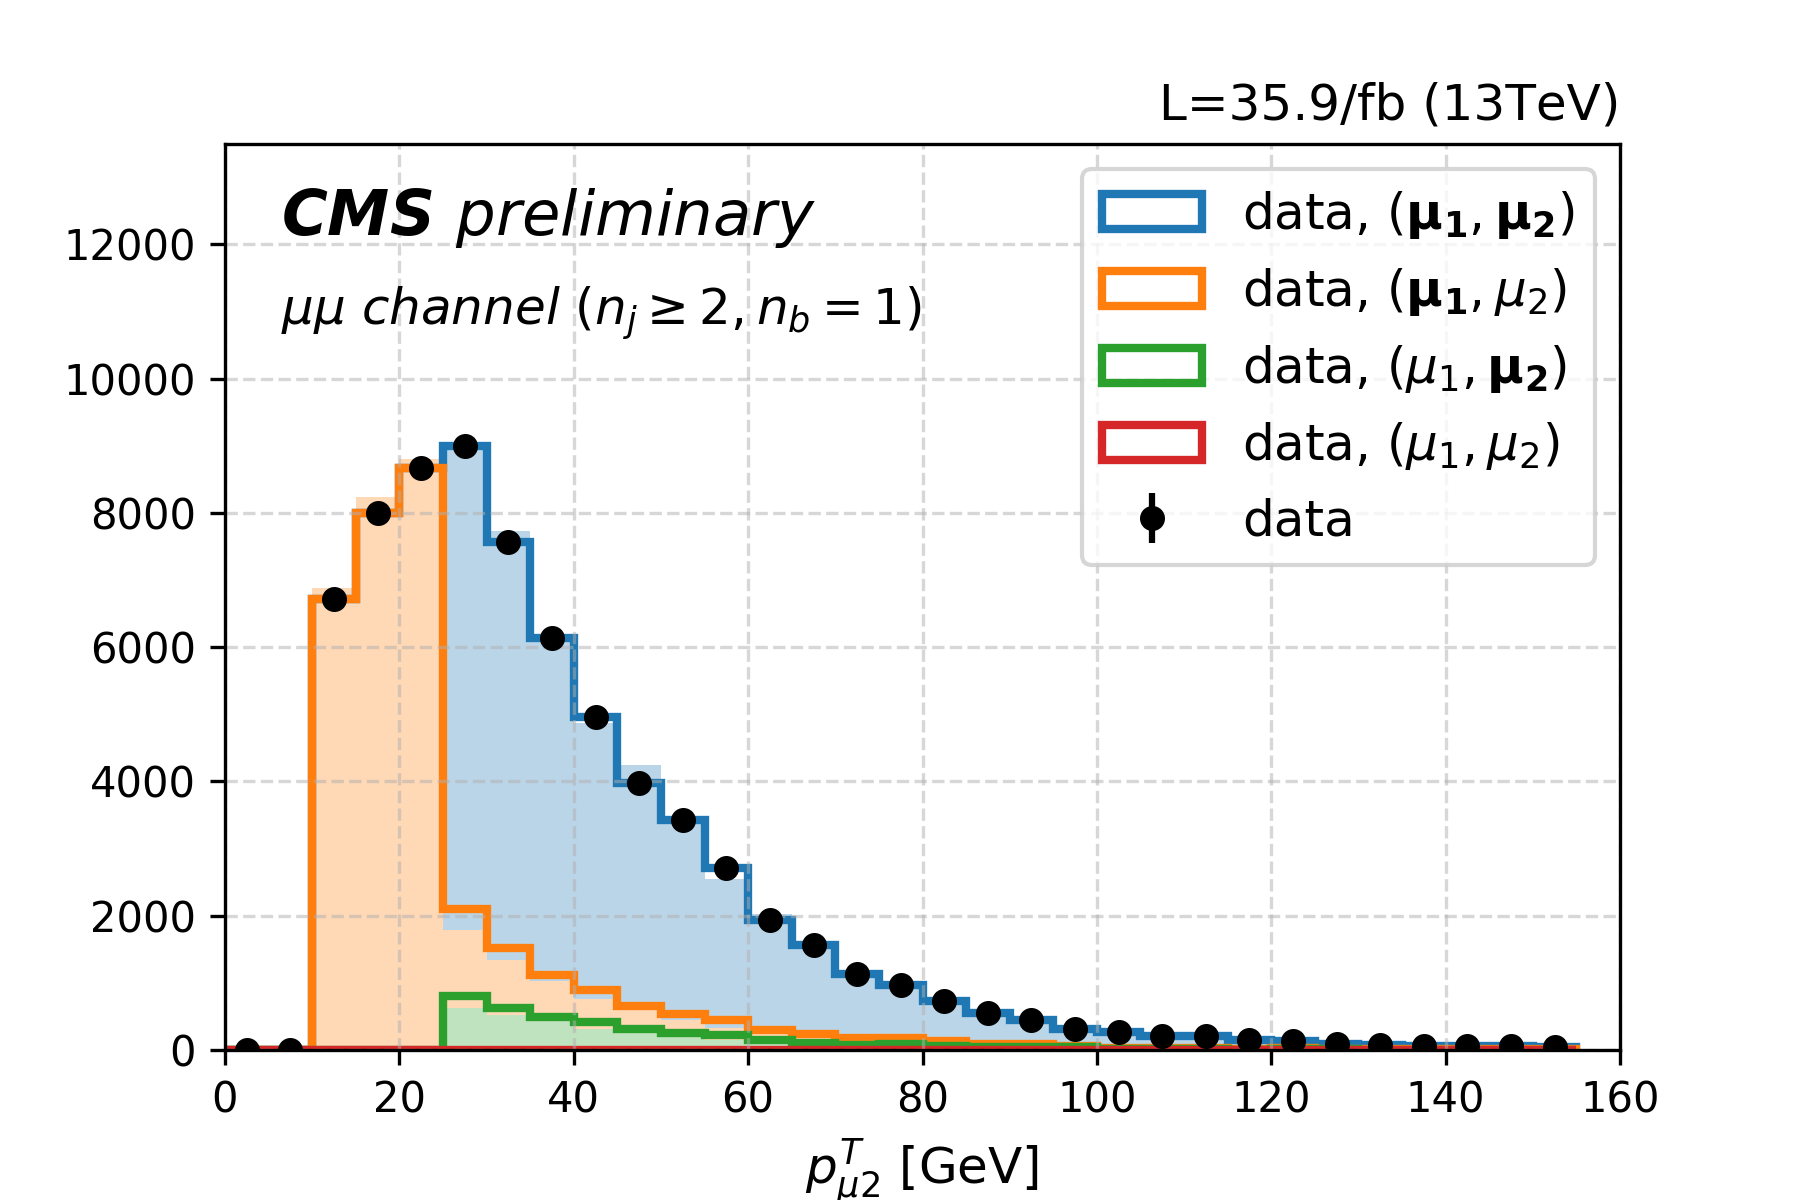
\includegraphics[width=0.49\textwidth]{chapters/Appendix/sectionTriggerTest/figures/trgLep_mumu.png}
  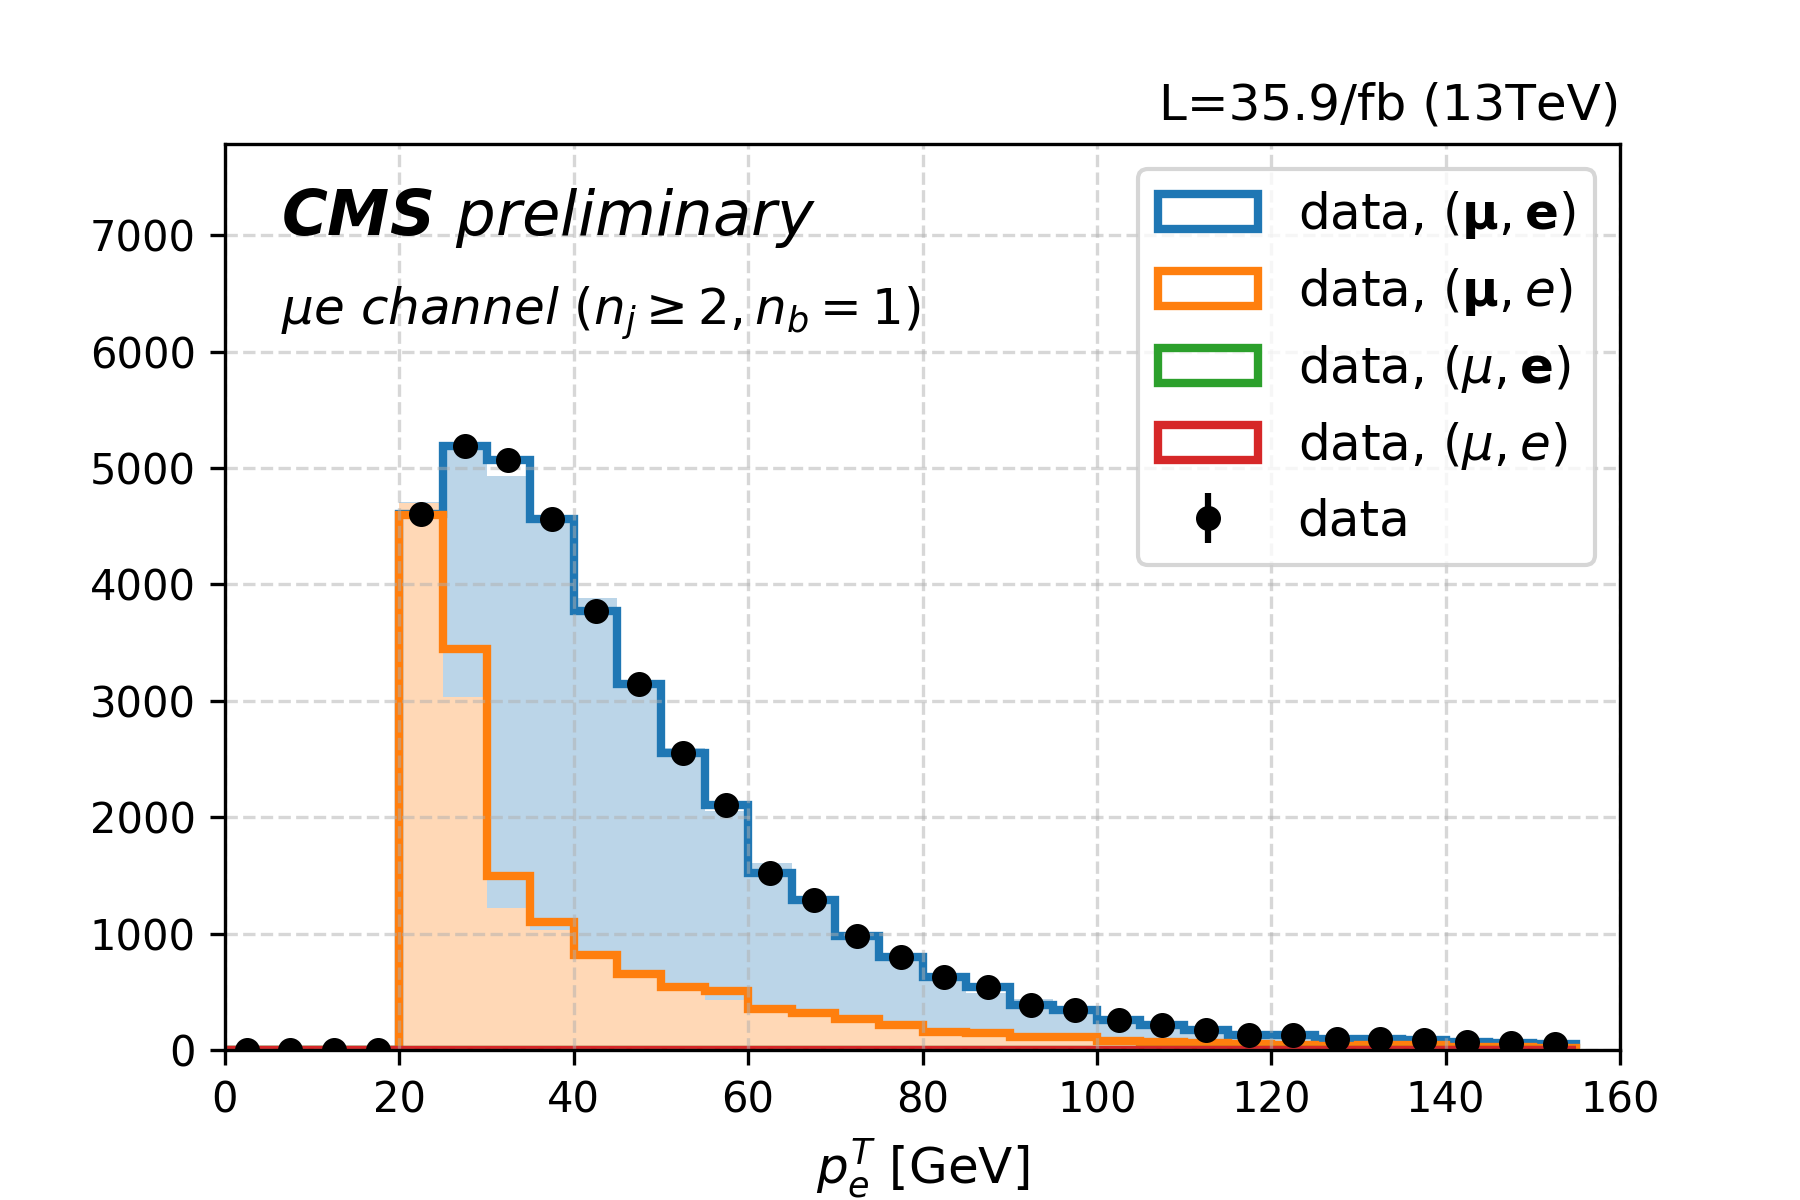
\includegraphics[width=0.49\textwidth]{chapters/Appendix/sectionTriggerTest/figures/trgLep_emu.png}
  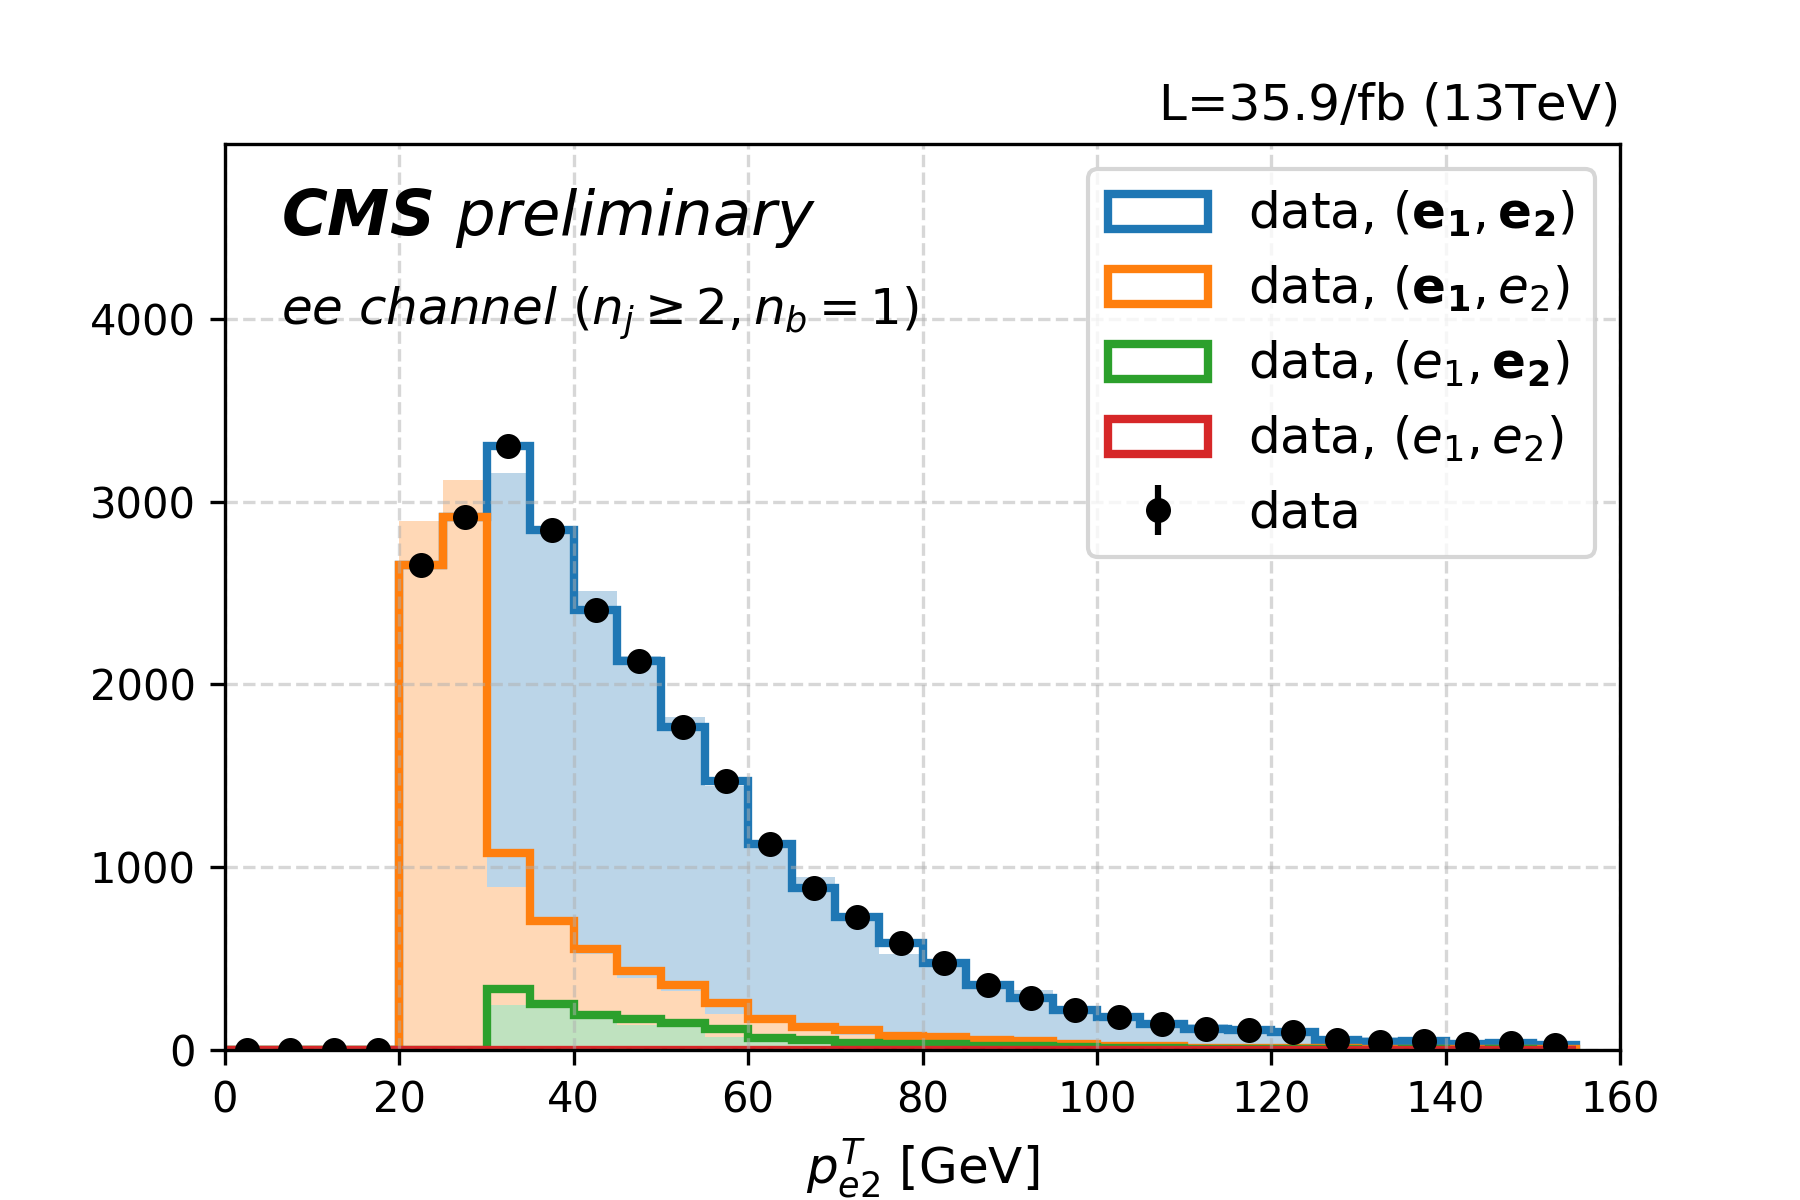
\includegraphics[width=0.49\textwidth]{chapters/Appendix/sectionTriggerTest/figures/trgLep_ee.png}
  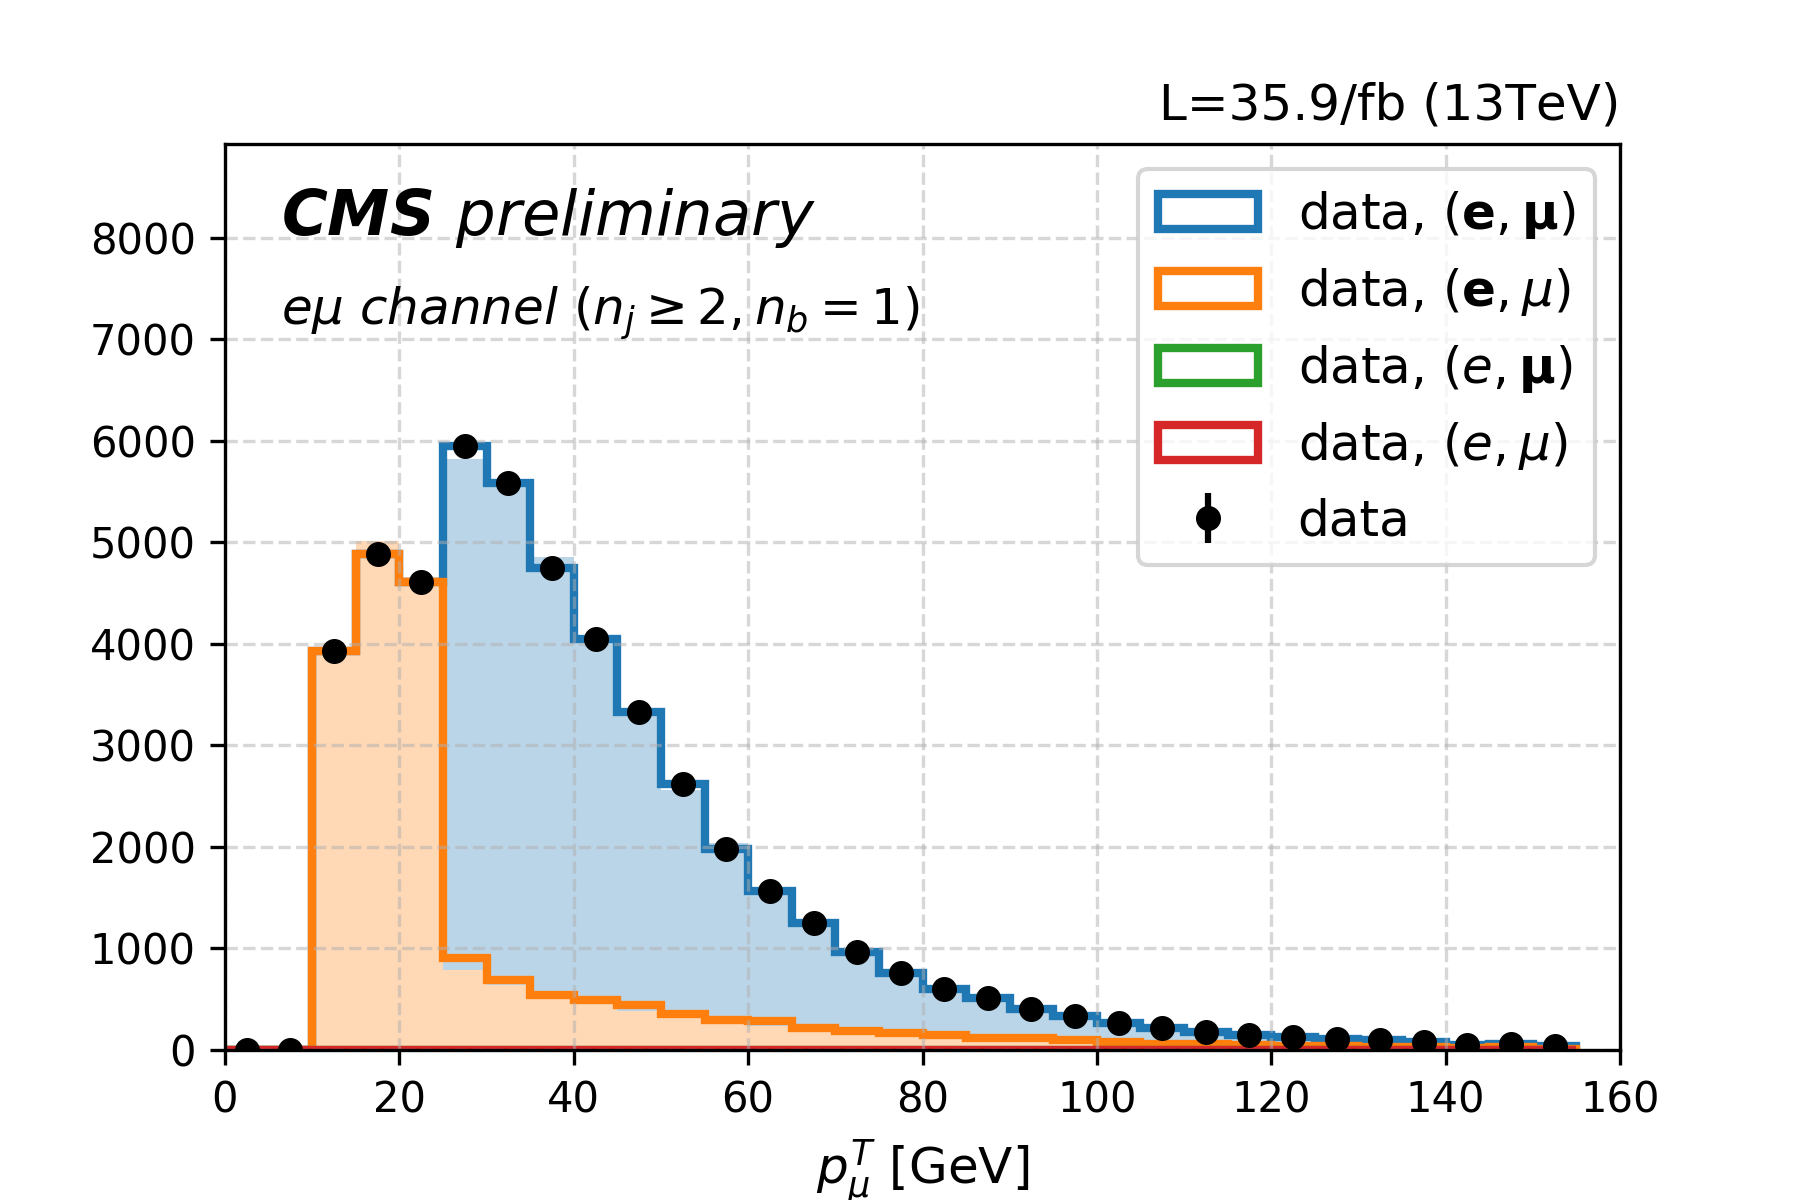
\includegraphics[width=0.49\textwidth]{chapters/Appendix/sectionTriggerTest/figures/trgLep_emu2.png}
  \caption{trailing lepton \pt in the $\mu\mu$,$ee$,$\mu e$,$e\mu$ channel. Data and MC events channel are split 
  based on the trigger test of leading and trailing lepton.
  \label{fig:triggerTest}}
\end{figure}
\FloatBarrier

\chapter{Reweight Dedicated TT MC Samples for the Estimation of theoretical uncertainties}

\begin{figure}
    \centering
    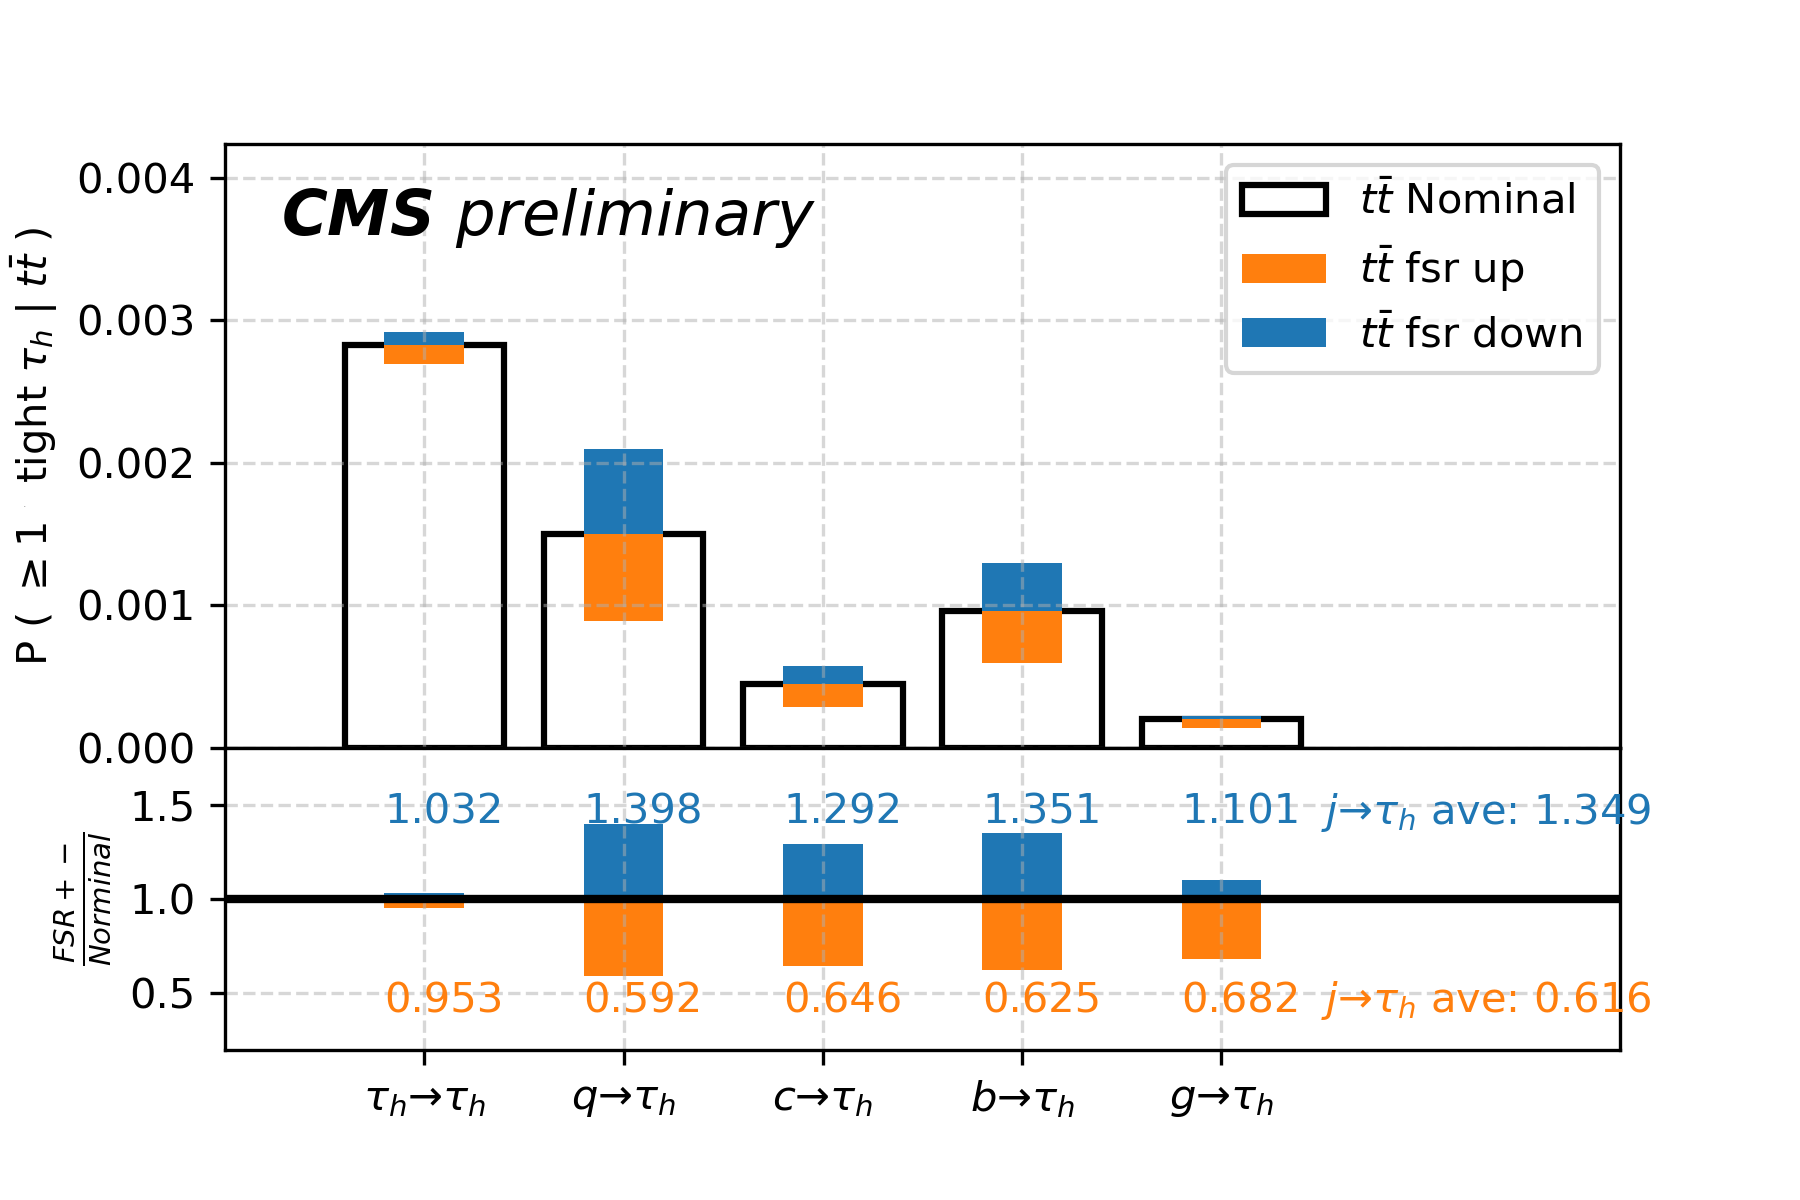
\includegraphics[width=0.49\textwidth]{chapters/Appendix/sectionTTSyst/figures/2020_MCRatio_fsr_tauGenFlavor_tauTight.png}
    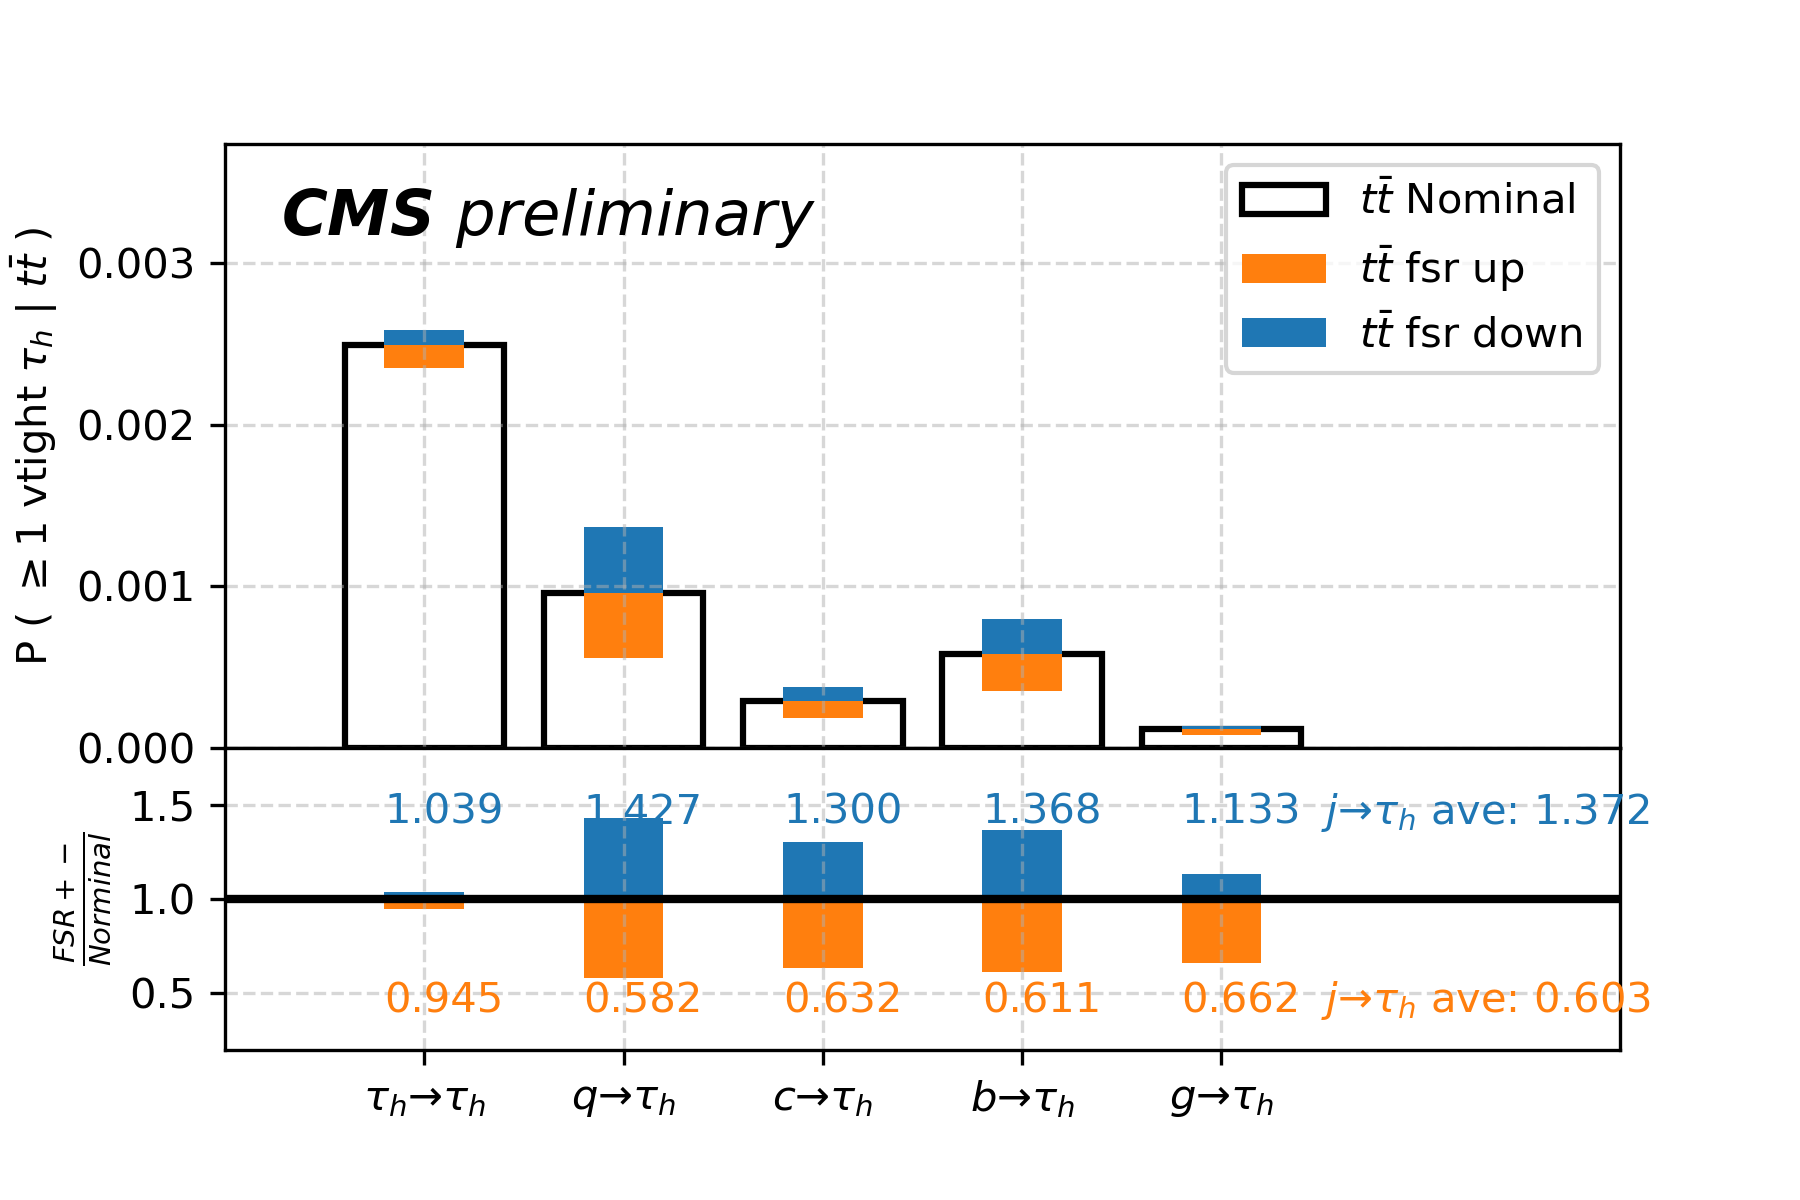
\includegraphics[width=0.49\textwidth]{chapters/Appendix/sectionTTSyst/figures/2020_MCRatio_fsr_tauGenFlavor_tauVTight.png}
    \caption{Reweight $\tau_h$ and $j \to \tau_h$ efficiencies in the dedicated FSR ttbar samples}
    \label{fig:appendix:reweighttt:sf}
\end{figure}

\begin{figure}
    \centering
    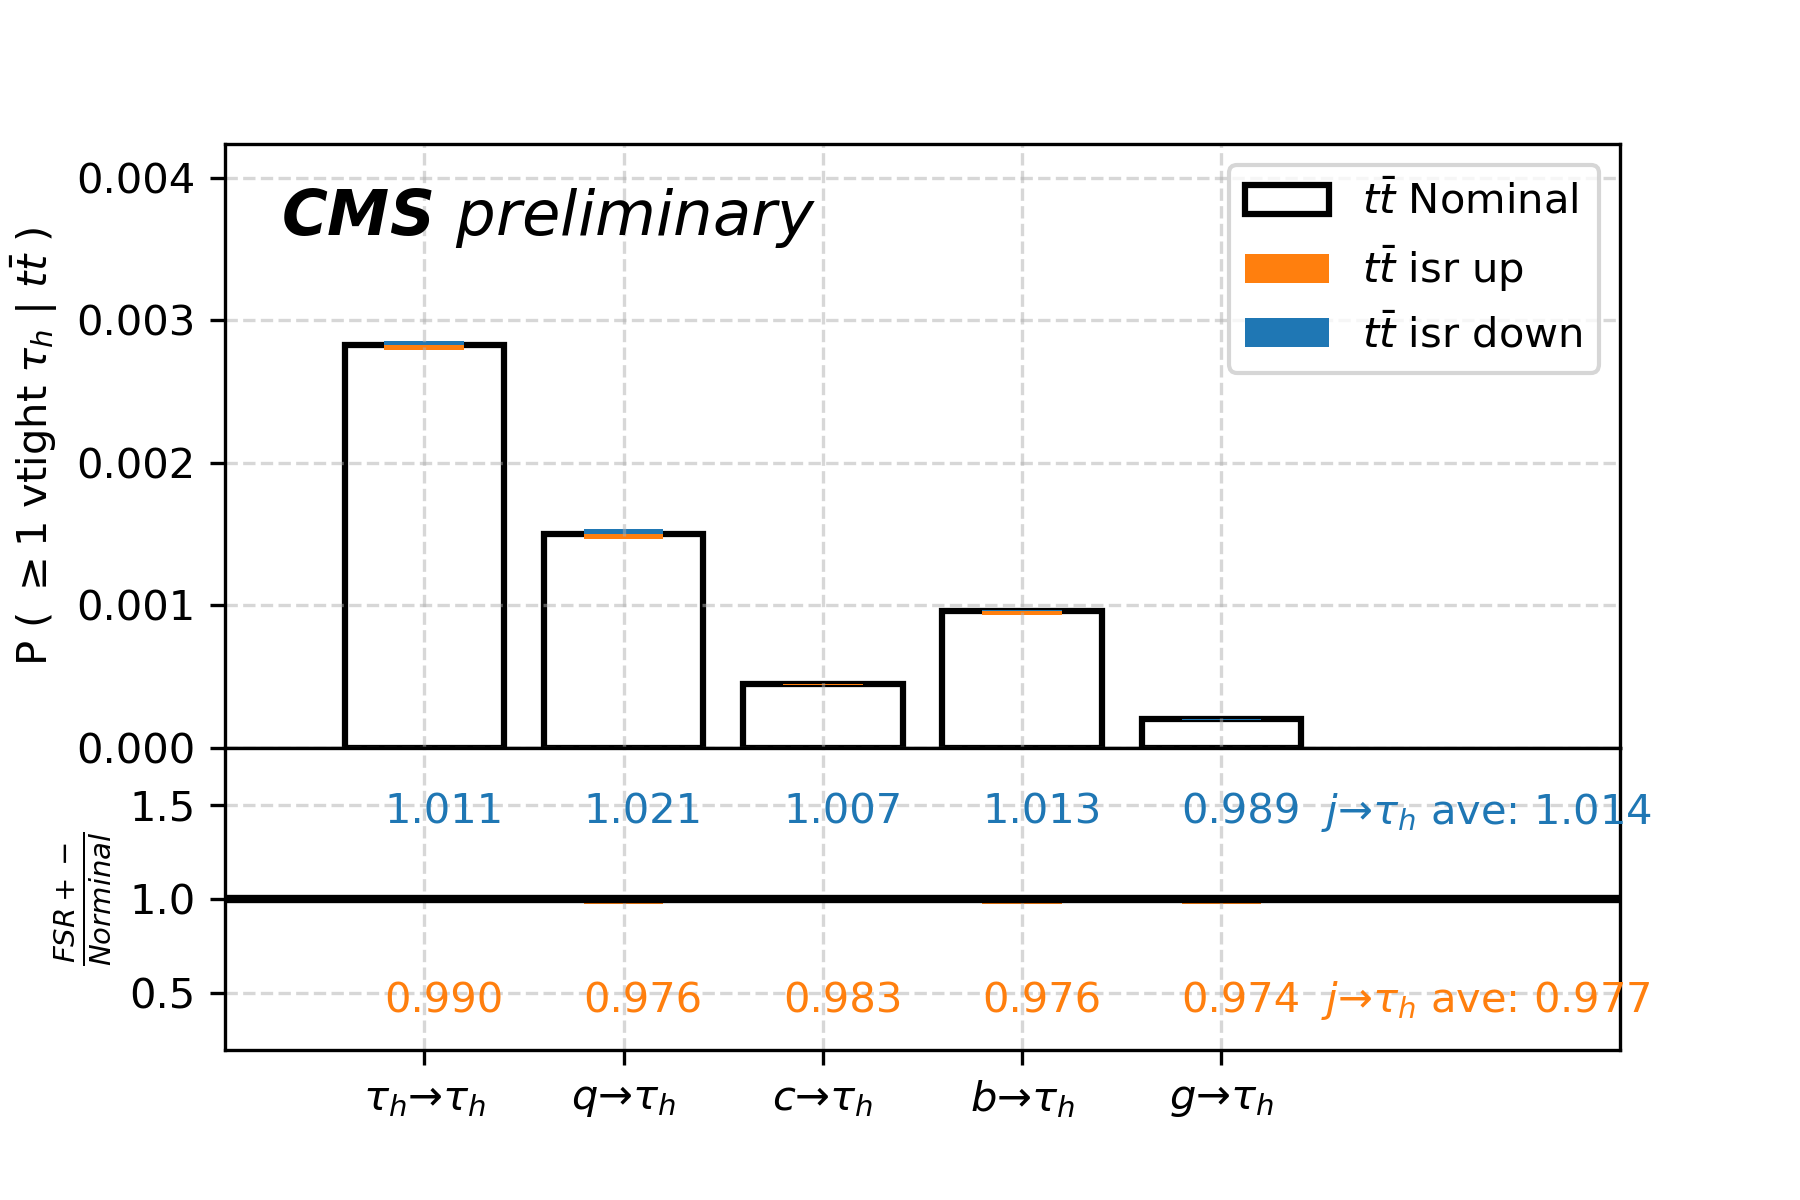
\includegraphics[width=0.49\textwidth]{chapters/Appendix/sectionTTSyst/figures/2020_MCRatio_isr_tauGenFlavor_tauTight.png}
    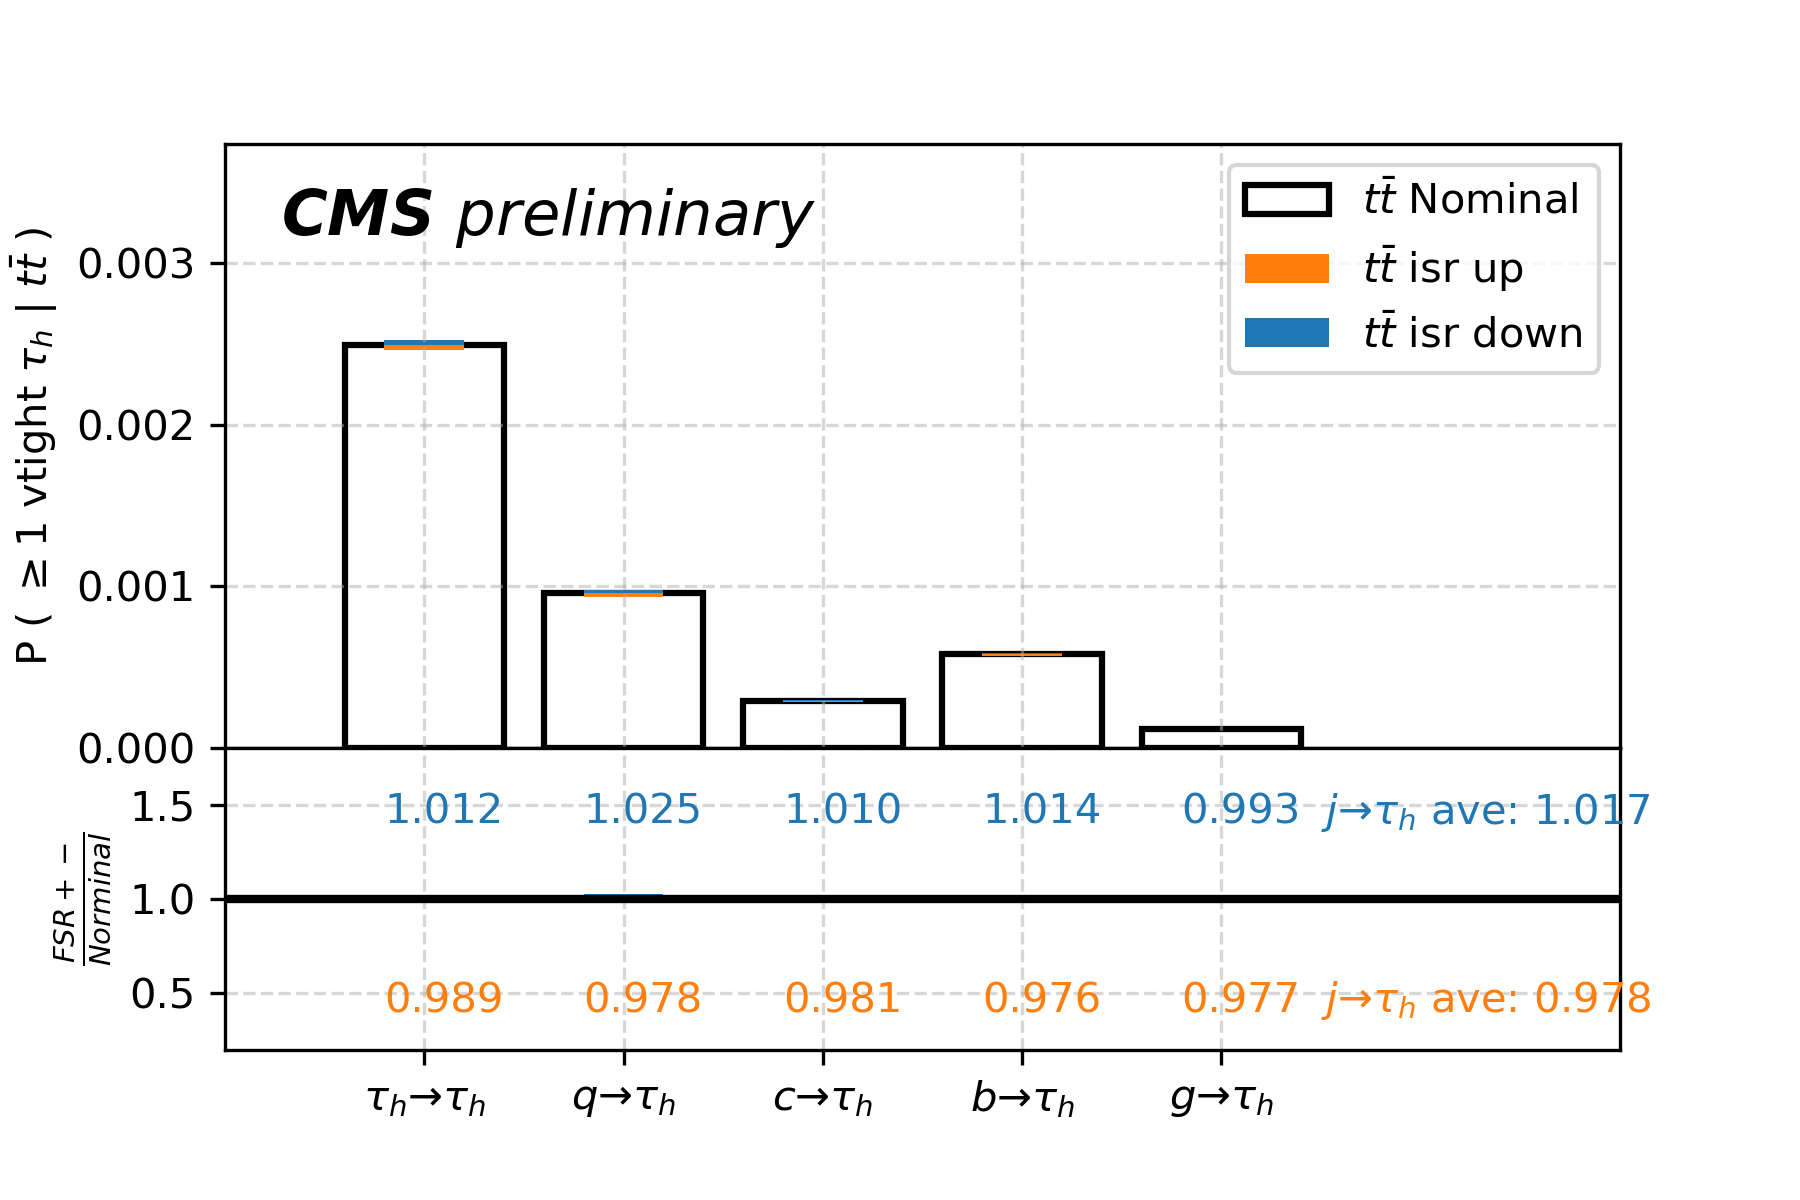
\includegraphics[width=0.49\textwidth]{chapters/Appendix/sectionTTSyst/figures/2020_MCRatio_isr_tauGenFlavor_tauVTight.png}
    \includegraphics[width=0.49\textwidth]{chapters/Appendix/sectionTTSyst/figures/2020_MCRatio_meps_tauGenFlavor_tauTight.png}
    \includegraphics[width=0.49\textwidth]{chapters/Appendix/sectionTTSyst/figures/2020_MCRatio_meps_tauGenFlavor_tauVTight.png}
    \includegraphics[width=0.49\textwidth]{chapters/Appendix/sectionTTSyst/figures/2020_MCRatio_ue_tauGenFlavor_tauTight.png}
    \includegraphics[width=0.49\textwidth]{chapters/Appendix/sectionTTSyst/figures/2020_MCRatio_ue_tauGenFlavor_tauVTight.png}
    \caption{Reweight $\tau_h$ and $j \to \tau_h$ efficiencies in the dedicated ISF, MEPS, UE ttbar samples}
    \label{fig:appendix:reweighttt:sf}
\end{figure}


\begin{figure}
    \centering
    \includegraphics[width=0.24\textwidth]{chapters/Appendix/sectionTTSyst/figures/afterCorr/icata0_ch0_fsr.png}
    \includegraphics[width=0.24\textwidth]{chapters/Appendix/sectionTTSyst/figures/afterCorr/icata0_ch1_fsr.png}
    \includegraphics[width=0.24\textwidth]{chapters/Appendix/sectionTTSyst/figures/afterCorr/icata0_ch2_fsr.png}
    \includegraphics[width=0.24\textwidth]{chapters/Appendix/sectionTTSyst/figures/afterCorr/icata0_ch3_fsr.png}

    \includegraphics[width=0.24\textwidth]{chapters/Appendix/sectionTTSyst/figures/afterCorr/icata1_ch0_fsr.png}
    \includegraphics[width=0.24\textwidth]{chapters/Appendix/sectionTTSyst/figures/afterCorr/icata1_ch1_fsr.png}
    \includegraphics[width=0.24\textwidth]{chapters/Appendix/sectionTTSyst/figures/afterCorr/icata1_ch2_fsr.png}
    \includegraphics[width=0.24\textwidth]{chapters/Appendix/sectionTTSyst/figures/afterCorr/icata1_ch3_fsr.png}
    
    \includegraphics[width=0.24\textwidth]{chapters/Appendix/sectionTTSyst/figures/afterCorr/icata2_ch0_fsr.png}
    \includegraphics[width=0.24\textwidth]{chapters/Appendix/sectionTTSyst/figures/afterCorr/icata2_ch1_fsr.png}
    \includegraphics[width=0.24\textwidth]{chapters/Appendix/sectionTTSyst/figures/afterCorr/icata2_ch2_fsr.png}
    \includegraphics[width=0.24\textwidth]{chapters/Appendix/sectionTTSyst/figures/afterCorr/icata2_ch3_fsr.png}

    \includegraphics[width=0.24\textwidth]{chapters/Appendix/sectionTTSyst/figures/afterCorr/icata3_ch0_fsr.png}
    \includegraphics[width=0.24\textwidth]{chapters/Appendix/sectionTTSyst/figures/afterCorr/icata3_ch1_fsr.png}
    \includegraphics[width=0.24\textwidth]{chapters/Appendix/sectionTTSyst/figures/afterCorr/icata3_ch2_fsr.png}
    \includegraphics[width=0.24\textwidth]{chapters/Appendix/sectionTTSyst/figures/afterCorr/icata3_ch3_fsr.png}
    
    \caption{Reweight $\tau_h$ and $j \to \tau_h$ efficiencies in the dedicated FSR, ISF, MEPS, UE ttbar samples}
    \label{fig:appendix:reweighttt:effAfterCorrFSR}
\end{figure}



\begin{figure}
    \centering
    \includegraphics[width=0.24\textwidth]{chapters/Appendix/sectionTTSyst/figures/afterCorr/icata0_ch0_isr.png}
    \includegraphics[width=0.24\textwidth]{chapters/Appendix/sectionTTSyst/figures/afterCorr/icata0_ch1_isr.png}
    \includegraphics[width=0.24\textwidth]{chapters/Appendix/sectionTTSyst/figures/afterCorr/icata0_ch2_isr.png}
    \includegraphics[width=0.24\textwidth]{chapters/Appendix/sectionTTSyst/figures/afterCorr/icata0_ch3_isr.png}

    \includegraphics[width=0.24\textwidth]{chapters/Appendix/sectionTTSyst/figures/afterCorr/icata1_ch0_isr.png}
    \includegraphics[width=0.24\textwidth]{chapters/Appendix/sectionTTSyst/figures/afterCorr/icata1_ch1_isr.png}
    \includegraphics[width=0.24\textwidth]{chapters/Appendix/sectionTTSyst/figures/afterCorr/icata1_ch2_isr.png}
    \includegraphics[width=0.24\textwidth]{chapters/Appendix/sectionTTSyst/figures/afterCorr/icata1_ch3_isr.png}
    
    \includegraphics[width=0.24\textwidth]{chapters/Appendix/sectionTTSyst/figures/afterCorr/icata2_ch0_isr.png}
    \includegraphics[width=0.24\textwidth]{chapters/Appendix/sectionTTSyst/figures/afterCorr/icata2_ch1_isr.png}
    \includegraphics[width=0.24\textwidth]{chapters/Appendix/sectionTTSyst/figures/afterCorr/icata2_ch2_isr.png}
    \includegraphics[width=0.24\textwidth]{chapters/Appendix/sectionTTSyst/figures/afterCorr/icata2_ch3_isr.png}

    \includegraphics[width=0.24\textwidth]{chapters/Appendix/sectionTTSyst/figures/afterCorr/icata3_ch0_isr.png}
    \includegraphics[width=0.24\textwidth]{chapters/Appendix/sectionTTSyst/figures/afterCorr/icata3_ch1_isr.png}
    \includegraphics[width=0.24\textwidth]{chapters/Appendix/sectionTTSyst/figures/afterCorr/icata3_ch2_isr.png}
    \includegraphics[width=0.24\textwidth]{chapters/Appendix/sectionTTSyst/figures/afterCorr/icata3_ch3_isr.png}
    
    \caption{Reweight $\tau_h$ and $j \to \tau_h$ efficiencies in the dedicated FSR, ISF, MEPS, UE ttbar samples}
    \label{fig:appendix:reweighttt:effAfterCorrFSR}
\end{figure}




\begin{figure}
    \centering
    \includegraphics[width=0.24\textwidth]{chapters/Appendix/sectionTTSyst/figures/afterCorr/icata0_ch0_meps.png}
    \includegraphics[width=0.24\textwidth]{chapters/Appendix/sectionTTSyst/figures/afterCorr/icata0_ch1_meps.png}
    \includegraphics[width=0.24\textwidth]{chapters/Appendix/sectionTTSyst/figures/afterCorr/icata0_ch2_meps.png}
    \includegraphics[width=0.24\textwidth]{chapters/Appendix/sectionTTSyst/figures/afterCorr/icata0_ch3_meps.png}

    \includegraphics[width=0.24\textwidth]{chapters/Appendix/sectionTTSyst/figures/afterCorr/icata1_ch0_meps.png}
    \includegraphics[width=0.24\textwidth]{chapters/Appendix/sectionTTSyst/figures/afterCorr/icata1_ch1_meps.png}
    \includegraphics[width=0.24\textwidth]{chapters/Appendix/sectionTTSyst/figures/afterCorr/icata1_ch2_meps.png}
    \includegraphics[width=0.24\textwidth]{chapters/Appendix/sectionTTSyst/figures/afterCorr/icata1_ch3_meps.png}
    
    \includegraphics[width=0.24\textwidth]{chapters/Appendix/sectionTTSyst/figures/afterCorr/icata2_ch0_meps.png}
    \includegraphics[width=0.24\textwidth]{chapters/Appendix/sectionTTSyst/figures/afterCorr/icata2_ch1_meps.png}
    \includegraphics[width=0.24\textwidth]{chapters/Appendix/sectionTTSyst/figures/afterCorr/icata2_ch2_meps.png}
    \includegraphics[width=0.24\textwidth]{chapters/Appendix/sectionTTSyst/figures/afterCorr/icata2_ch3_meps.png}

    \includegraphics[width=0.24\textwidth]{chapters/Appendix/sectionTTSyst/figures/afterCorr/icata3_ch0_meps.png}
    \includegraphics[width=0.24\textwidth]{chapters/Appendix/sectionTTSyst/figures/afterCorr/icata3_ch1_meps.png}
    \includegraphics[width=0.24\textwidth]{chapters/Appendix/sectionTTSyst/figures/afterCorr/icata3_ch2_meps.png}
    \includegraphics[width=0.24\textwidth]{chapters/Appendix/sectionTTSyst/figures/afterCorr/icata3_ch3_meps.png}
    
    \caption{Reweight $\tau_h$ and $j \to \tau_h$ efficiencies in the dedicated FSR, ISF, MEPS, UE ttbar samples}
    \label{fig:appendix:reweighttt:effAfterCorrFSR}
\end{figure}


\begin{figure}
    \centering
    \includegraphics[width=0.24\textwidth]{chapters/Appendix/sectionTTSyst/figures/afterCorr/icata0_ch0_ue.png}
    \includegraphics[width=0.24\textwidth]{chapters/Appendix/sectionTTSyst/figures/afterCorr/icata0_ch1_ue.png}
    \includegraphics[width=0.24\textwidth]{chapters/Appendix/sectionTTSyst/figures/afterCorr/icata0_ch2_ue.png}
    \includegraphics[width=0.24\textwidth]{chapters/Appendix/sectionTTSyst/figures/afterCorr/icata0_ch3_ue.png}

    \includegraphics[width=0.24\textwidth]{chapters/Appendix/sectionTTSyst/figures/afterCorr/icata1_ch0_ue.png}
    \includegraphics[width=0.24\textwidth]{chapters/Appendix/sectionTTSyst/figures/afterCorr/icata1_ch1_ue.png}
    \includegraphics[width=0.24\textwidth]{chapters/Appendix/sectionTTSyst/figures/afterCorr/icata1_ch2_ue.png}
    \includegraphics[width=0.24\textwidth]{chapters/Appendix/sectionTTSyst/figures/afterCorr/icata1_ch3_ue.png}
    
    \includegraphics[width=0.24\textwidth]{chapters/Appendix/sectionTTSyst/figures/afterCorr/icata2_ch0_ue.png}
    \includegraphics[width=0.24\textwidth]{chapters/Appendix/sectionTTSyst/figures/afterCorr/icata2_ch1_ue.png}
    \includegraphics[width=0.24\textwidth]{chapters/Appendix/sectionTTSyst/figures/afterCorr/icata2_ch2_ue.png}
    \includegraphics[width=0.24\textwidth]{chapters/Appendix/sectionTTSyst/figures/afterCorr/icata2_ch3_ue.png}

    \includegraphics[width=0.24\textwidth]{chapters/Appendix/sectionTTSyst/figures/afterCorr/icata3_ch0_ue.png}
    \includegraphics[width=0.24\textwidth]{chapters/Appendix/sectionTTSyst/figures/afterCorr/icata3_ch1_ue.png}
    \includegraphics[width=0.24\textwidth]{chapters/Appendix/sectionTTSyst/figures/afterCorr/icata3_ch2_ue.png}
    \includegraphics[width=0.24\textwidth]{chapters/Appendix/sectionTTSyst/figures/afterCorr/icata3_ch3_ue.png}
    
    \caption{Reweight $\tau_h$ and $j \to \tau_h$ efficiencies in the dedicated FSR, ISF, MEPS, UE ttbar samples}
    \label{fig:appendix:reweighttt:effAfterCorrFSR}
\end{figure}



Converting the distriution of branching fractions to the distribution of
ratios of branching fractions requires some care given the significant
correlation between the branching fractions.  The procedure is
nonetheless straight forward and has been carried in statistics
literature for the one dimensional case~\cite{10.1093/biomet/24.3-4.428,
10.2307/2334671}.  The procedure of transforming variables is the same
for the two dimensional case, namely, calculate the expectation value of
the absolute value of the branching fraction in the denominator.  Given
the derivation is straight forward, the result is quoted here without
going through all of the steps.  Starting from the pdf of the leptonic
branching fractions,

\begin{equation}
    g(\beta_{e}, \beta_{\mu}, \beta_{\tau}) =
    \mathcal{N}\left(\boldsymbol{\beta}; \hat{\boldsymbol{\beta}}, \boldsymbol{\Sigma}\right)
\end{equation}

where $\hat{\boldsymbol{\beta}}$ is the maximum likelihood estimates of the
leptonic branching fractions and $\boldsymbol{\Sigma}$ is the covariance.
The transformation to the PDF of the ratios is then found by evaluating
the integral,


\section{Ratios of Branching Fraction}

\begin{equation}
    f(r_{e\tau}, r_{\mu\tau}) = \int_{-\infty}^{\infty}
    \left| \beta_{\tau}\right|g(r_{e\tau}\beta_{\tau}, r_{\mu\tau}\beta_{\tau}, \beta_{\tau})
    d\beta_{\tau}
\end{equation}

Carrying out the integration is very similar to the one dimensional
case.  The resulting expression is,

\begin{equation}
    f(r_{e\tau}, r_{\mu\tau}) 
    = \frac{bd}{2\pi \sigma_{e}\sigma_{\mu}\sigma_{\tau} a^{3}}
        \left[ \Phi \left(\frac{b}{a\sqrt{\Psi}}\right)
         - \Phi\left(\frac{b}{a\sqrt{\Psi}}\right)\right] 
         +
         \frac{\sqrt{\Psi}}{\sqrt{2\pi^{3}}\sigma_{e}\sigma_{\mu}\sigma_{\tau}}e^{-\frac{c}{2\Psi}},
\end{equation}

where,

\begin{align} 
    a \equiv a\left(r_{e\tau}, r_{\mu\tau}\right) 
            &= \frac{r_{e\tau}^{2}\left(1 - \rho_{\mu\tau} \right)}{\sigma_{e}^{2}}
            + \frac{r_{\mu\tau}^{2}\left(1 - \rho_{e\tau} \right)}{\sigma_{\mu}^{2}}
            + \frac{\left(1 - \rho_{e\mu} \right)}{\sigma_{\tau}^{2}} \\
            \nonumber
            &+ \frac{2r_{e\tau}r_{\mu\tau}\left( \rho_{e\tau} \rho_{\mu\tau}   - \rho_{e\mu} \right)}{\sigma_{e}\sigma_{\mu}} 
            \nonumber
            + \frac{2r_{e\tau}\left( \rho_{e\mu} \rho_{\mu\tau}   - \rho_{e\tau} \right)}{\sigma_{e}\sigma_{\tau}} \\
            \nonumber
            &+ \frac{2r_{\mu\tau}\left( \rho_{e\mu} \rho_{e\tau}   - \rho_{\mu\tau} \right)}{\sigma_{\mu}\sigma_{\tau}}
\end{align}
\begin{align}
    b \equiv b(r_{e\tau}, r_{\mu\tau}) 
        &= \frac{r_{e\tau}\beta_{e}\left(1 - \rho_{\mu\tau} \right)}{\sigma_{e}^{2}}
        + \frac{r_{\mu\tau}\beta_{\mu}\left(1 - \rho_{e\tau} \right)}{\sigma_{\mu}^{2}}
        + \frac{\beta_{\tau}\left(1 - \rho_{e\mu} \right)}{\sigma_{\tau}^{2}} \\
        \nonumber
        &+ \frac{\left(r_{e\tau}\beta_{\mu} + r_{\mu\tau}\beta_{e}\right)\left( \rho_{e\tau} \rho_{\mu\tau} - \rho_{e\mu} \right)}{\sigma_{e}\sigma_{\mu}}
        \nonumber
        + \frac{\left(r_{e\tau}\beta_{\tau} + \beta_{e}\right)\left( \rho_{e\mu} \rho_{\mu\tau}   - \rho_{e\tau} \right)}{\sigma_{e}\sigma_{\tau}} \\ 
        \nonumber
        &+ \frac{\left(r_{\mu\tau}\beta_{\tau} + \beta_{\mu}\right)\left( \rho_{e\tau} \rho_{e\mu}   - \rho_{\mu\tau} \right)}{\sigma_{\mu}\sigma_{\tau}}
\end{align}
\begin{align}
    c &= \frac{\beta_{e}^{2}\left(1 - \rho_{\mu\tau} \right)}{\sigma_{e}^{2}}
    + \frac{\beta_{\mu}^{2}\left(1 - \rho_{e\tau} \right)}{\sigma_{\mu}^{2}}
    + \frac{\beta_{\tau}^{2}\left(1 - \rho_{e\mu} \right)}{\sigma_{\tau}^{2}} \\
        \nonumber
        &+ \frac{2\beta_{e}\beta_{\mu}\left( \rho_{e\tau} \rho_{\mu\tau} - \rho_{e\mu} \right)}{\sigma_{e}\sigma_{\mu}}
        \nonumber
        + \frac{2\beta_{e}\beta_{\tau}\left( \rho_{e\mu} \rho_{\mu\tau}   - \rho_{e\tau} \right)}{\sigma_{e}\sigma_{\tau}} \\ 
        \nonumber
        &+ \frac{2\beta_{\mu}\beta_{\tau}\left( \rho_{e\tau} \rho_{e\mu}   - \rho_{\mu\tau} \right)}{\sigma_{\mu}\sigma_{\tau}}
\end{align}

\begin{equation}
    \Psi = 1 - \rho_{e\mu}^{2} - \rho_{e\tau}^{2} - \rho_{\mu\tau}^{2} + 2\rho_{e\mu}\rho_{e\tau}\rho_{\mu\tau}
\end{equation}

This expression gives the analytic expression for the PDF of two ratios
derived from three normally distributed quantities accounting for their
correlations and is used in drawing figure~\ref{fig:ratio_contours_2D}.
\FloatBarrier
\section{Estimation of QCD in the $l\tau$ and $l\rm{jet}$ channel}


\begin{figure}
    \centering
    \includegraphics[width=0.24\textwidth]{chapters/Appendix/sectionQCD/figures/mutau_==0_==0_dilepton_mass.png}
    \includegraphics[width=0.24\textwidth]{chapters/Appendix/sectionQCD/figures/mutau_ss_==0_==0_dilepton_mass.png}
    \includegraphics[width=0.24\textwidth]{chapters/Appendix/sectionQCD/figures/etau_==0_==0_dilepton_mass.png}
    \includegraphics[width=0.24\textwidth]{chapters/Appendix/sectionQCD/figures/etau_ss_==0_==0_dilepton_mass.png}
    
    \includegraphics[width=0.24\textwidth]{chapters/Appendix/sectionQCD/figures/mutau_==1_==0_dilepton_mass.png}
    \includegraphics[width=0.24\textwidth]{chapters/Appendix/sectionQCD/figures/mutau_ss_==1_==0_dilepton_mass.png}
    \includegraphics[width=0.24\textwidth]{chapters/Appendix/sectionQCD/figures/etau_==1_==0_dilepton_mass.png}
    \includegraphics[width=0.24\textwidth]{chapters/Appendix/sectionQCD/figures/etau_ss_==1_==0_dilepton_mass.png}
    
    \includegraphics[width=0.24\textwidth]{chapters/Appendix/sectionQCD/figures/mutau_==1_==1_dilepton_mass.png}
    \includegraphics[width=0.24\textwidth]{chapters/Appendix/sectionQCD/figures/mutau_ss_==1_==1_dilepton_mass.png}
    \includegraphics[width=0.24\textwidth]{chapters/Appendix/sectionQCD/figures/etau_==1_==1_dilepton_mass.png}
    \includegraphics[width=0.24\textwidth]{chapters/Appendix/sectionQCD/figures/etau_ss_==1_==1_dilepton_mass.png}
    
    \includegraphics[width=0.24\textwidth]{chapters/Appendix/sectionQCD/figures/mutau_>=2_==0_dilepton_mass.png}
    \includegraphics[width=0.24\textwidth]{chapters/Appendix/sectionQCD/figures/mutau_ss_>=2_==0_dilepton_mass.png}
    \includegraphics[width=0.24\textwidth]{chapters/Appendix/sectionQCD/figures/etau_>=2_==0_dilepton_mass.png}
    \includegraphics[width=0.24\textwidth]{chapters/Appendix/sectionQCD/figures/etau_ss_>=2_==0_dilepton_mass.png}
    
    
    \includegraphics[width=0.24\textwidth]{chapters/Appendix/sectionQCD/figures/mutau_>=2_==1_dilepton_mass.png}
    \includegraphics[width=0.24\textwidth]{chapters/Appendix/sectionQCD/figures/mutau_ss_>=2_==1_dilepton_mass.png}
    \includegraphics[width=0.24\textwidth]{chapters/Appendix/sectionQCD/figures/etau_>=2_==1_dilepton_mass.png}
    \includegraphics[width=0.24\textwidth]{chapters/Appendix/sectionQCD/figures/etau_ss_>=2_==1_dilepton_mass.png}
    
    
    \includegraphics[width=0.24\textwidth]{chapters/Appendix/sectionQCD/figures/mutau_>=2_>=2_dilepton_mass.png}
    \includegraphics[width=0.24\textwidth]{chapters/Appendix/sectionQCD/figures/mutau_ss_>=2_>=2_dilepton_mass.png}
    \includegraphics[width=0.24\textwidth]{chapters/Appendix/sectionQCD/figures/etau_>=2_>=2_dilepton_mass.png}
    \includegraphics[width=0.24\textwidth]{chapters/Appendix/sectionQCD/figures/etau_ss_>=2_>=2_dilepton_mass.png}
    
    

    \caption{The $m_{l\tau}$ in the SS and OS region of $\mu\tau$ (left two columns) and $e\tau$ (right two columns) 
    channel. Different rows correspond to different $n_j,n_b$ configuration, which includes
    $n_j=0,n_b=0$, $n_j=1,n_b=0$, $n_j=1,n_b=1$, $n_j\geq 2,n_b=0$, $n_j\geq 2,n_b=1$, $n_j\geq 2,n_b\geq 2$, 
    from the first to the last row. The last two rows dominated by \ttbar are the channels used by the counting analysis.
    }
    \label{fig:appendix:qcdsf:ltau}
\end{figure}



\begin{figure}
    \centering
    \includegraphics[width=0.24\textwidth]{chapters/Appendix/sectionQCD/figures/123j1b/mu_leptonOnePt_True.png}
    \includegraphics[width=0.24\textwidth]{chapters/Appendix/sectionQCD/figures/123j1b/mu_leptonOnePt_False.png}
    \includegraphics[width=0.24\textwidth]{chapters/Appendix/sectionQCD/figures/123j1b/e_leptonOnePt_True.png}
    \includegraphics[width=0.24\textwidth]{chapters/Appendix/sectionQCD/figures/123j1b/e_leptonOnePt_False.png}
    
    \includegraphics[width=0.24\textwidth]{chapters/Appendix/sectionQCD/figures/123j1b/mu_leptonOneEta_True.png}
    \includegraphics[width=0.24\textwidth]{chapters/Appendix/sectionQCD/figures/123j1b/mu_leptonOneEta_False.png}
    \includegraphics[width=0.24\textwidth]{chapters/Appendix/sectionQCD/figures/123j1b/e_leptonOneEta_True.png}
    \includegraphics[width=0.24\textwidth]{chapters/Appendix/sectionQCD/figures/123j1b/e_leptonOneEta_False.png}
    
    \includegraphics[width=0.24\textwidth]{chapters/Appendix/sectionQCD/figures/123j1b/mu_nJets_True.png}
    \includegraphics[width=0.24\textwidth]{chapters/Appendix/sectionQCD/figures/123j1b/mu_nJets_False.png}
    \includegraphics[width=0.24\textwidth]{chapters/Appendix/sectionQCD/figures/123j1b/e_nJets_True.png}
    \includegraphics[width=0.24\textwidth]{chapters/Appendix/sectionQCD/figures/123j1b/e_nJets_False.png}
    
    \includegraphics[width=0.24\textwidth]{chapters/Appendix/sectionQCD/figures/123j1b/mu_nBJets_True.png}
    \includegraphics[width=0.24\textwidth]{chapters/Appendix/sectionQCD/figures/123j1b/mu_nBJets_False.png}
    \includegraphics[width=0.24\textwidth]{chapters/Appendix/sectionQCD/figures/123j1b/e_nBJets_True.png}
    \includegraphics[width=0.24\textwidth]{chapters/Appendix/sectionQCD/figures/123j1b/e_nBJets_False.png}
    

    \caption{The iso and anti-iso region of $\mu$+jet (left two columns) and $e$+jet (right two columns) channel 
    with $1\leq n_j <4, n_b\geq1$, which is orthogonal to the $n_j\geq4,n_b\geq1$ signal region.
    }
    \label{fig:appendix:123j1b}
\end{figure}


\begin{figure}
    \centering
    \includegraphics[width=0.49\textwidth]{chapters/Appendix/sectionQCD/figures/123j1b/SF_mu_1d.png}
    \includegraphics[width=0.49\textwidth]{chapters/Appendix/sectionQCD/figures/123j1b/SF_e_1d.png}
    \includegraphics[width=0.49\textwidth]{chapters/Appendix/sectionQCD/figures/123j1b/SF_mu_2d.png}
    \includegraphics[width=0.49\textwidth]{chapters/Appendix/sectionQCD/figures/123j1b/SF_e_2d.png}

    \caption{iso-to-antiiso SF in the $\mu$+jet (left) and $e$+jet (right) channel 
    with $1\leq n_j <4, n_b\geq1$ side-band region.}
    \label{fig:appendix:123j1b_sf}
\end{figure}



\begin{figure}
    \centering
    \includegraphics[width=0.24\textwidth]{chapters/Appendix/sectionQCD/figures/4j1b/mu_leptonOnePt_True_mcqcd.png}
    \includegraphics[width=0.24\textwidth]{chapters/Appendix/sectionQCD/figures/4j1b/mu_leptonOnePt_False.png}
    \includegraphics[width=0.24\textwidth]{chapters/Appendix/sectionQCD/figures/4j1b/e_leptonOnePt_True_mcqcd.png}
    \includegraphics[width=0.24\textwidth]{chapters/Appendix/sectionQCD/figures/4j1b/e_leptonOnePt_False.png}
    
    \includegraphics[width=0.24\textwidth]{chapters/Appendix/sectionQCD/figures/4j1b/mu_leptonOneEta_True_mcqcd.png}
    \includegraphics[width=0.24\textwidth]{chapters/Appendix/sectionQCD/figures/4j1b/mu_leptonOneEta_False.png}
    \includegraphics[width=0.24\textwidth]{chapters/Appendix/sectionQCD/figures/4j1b/e_leptonOneEta_True_mcqcd.png}
    \includegraphics[width=0.24\textwidth]{chapters/Appendix/sectionQCD/figures/4j1b/e_leptonOneEta_False.png}
    
    \includegraphics[width=0.24\textwidth]{chapters/Appendix/sectionQCD/figures/4j1b/mu_nJets_True_mcqcd.png}
    \includegraphics[width=0.24\textwidth]{chapters/Appendix/sectionQCD/figures/4j1b/mu_nJets_False.png}
    \includegraphics[width=0.24\textwidth]{chapters/Appendix/sectionQCD/figures/4j1b/e_nJets_True_mcqcd.png}
    \includegraphics[width=0.24\textwidth]{chapters/Appendix/sectionQCD/figures/4j1b/e_nJets_False.png}
    
    \includegraphics[width=0.24\textwidth]{chapters/Appendix/sectionQCD/figures/4j1b/mu_nBJets_True_mcqcd.png}
    \includegraphics[width=0.24\textwidth]{chapters/Appendix/sectionQCD/figures/4j1b/mu_nBJets_False.png}
    \includegraphics[width=0.24\textwidth]{chapters/Appendix/sectionQCD/figures/4j1b/e_nBJets_True_mcqcd.png}
    \includegraphics[width=0.24\textwidth]{chapters/Appendix/sectionQCD/figures/4j1b/e_nBJets_False.png}
    

    \caption{The iso and anti-iso region of $\mu$+jet (left two columns) and $e$+jet (right two columns) channel 
    with $n_j\geq4,n_b\geq1$, the signal region.}
    \label{fig:appendix:4j1b}
\end{figure}
\FloatBarrier





% 2
% --------------------------------------------------
\chapter{Plots for $Br(W)$ Analysis}



\section{Kinematics Plots in Counting Analysis}


%  emu channel
\begin{figure}[ht]
    \centering
    $ \mu  e - 1b$ \\
    \includegraphics[width=0.49\textwidth]{chapters/Appendix/sectionPlots/figures/kinematics_pickles/emu/1b/emu_1b_lepton1_pt.pdf}
    \includegraphics[width=0.49\textwidth]{chapters/Appendix/sectionPlots/figures/kinematics_pickles/emu/1b/emu_1b_lepton1_eta.pdf}
    \includegraphics[width=0.49\textwidth]{chapters/Appendix/sectionPlots/figures/kinematics_pickles/emu/1b/emu_1b_lepton2_pt.pdf}
    \includegraphics[width=0.49\textwidth]{chapters/Appendix/sectionPlots/figures/kinematics_pickles/emu/1b/emu_1b_lepton2_eta.pdf}
    \includegraphics[width=0.49\textwidth]{chapters/Appendix/sectionPlots/figures/kinematics_pickles/emu/1b/emu_1b_nJets.pdf}
    \includegraphics[width=0.49\textwidth]{chapters/Appendix/sectionPlots/figures/kinematics_pickles/emu/1b/emu_1b_nBJets.pdf}
    
    \caption{$e\mu$ channel. Plots in 1b(2b) case are top(bottom) two rows.}
\end{figure}

\begin{figure}[ht]
    \centering
    $ \mu e- 2b$ \\
    \includegraphics[width=0.49\textwidth]{chapters/Appendix/sectionPlots/figures/kinematics_pickles/emu/2b/emu_2b_lepton1_pt.pdf}
    \includegraphics[width=0.49\textwidth]{chapters/Appendix/sectionPlots/figures/kinematics_pickles/emu/2b/emu_2b_lepton1_eta.pdf}
    \includegraphics[width=0.49\textwidth]{chapters/Appendix/sectionPlots/figures/kinematics_pickles/emu/2b/emu_2b_lepton2_pt.pdf}
    \includegraphics[width=0.49\textwidth]{chapters/Appendix/sectionPlots/figures/kinematics_pickles/emu/2b/emu_2b_lepton2_eta.pdf}
    \includegraphics[width=0.49\textwidth]{chapters/Appendix/sectionPlots/figures/kinematics_pickles/emu/2b/emu_2b_nJets.pdf}
    \includegraphics[width=0.49\textwidth]{chapters/Appendix/sectionPlots/figures/kinematics_pickles/emu/2b/emu_2b_nBJets.pdf}
    
    \caption{$e\mu$ channel. Plots in 1b(2b) case are top(bottom) two rows.}
\end{figure}

%  mumu channel
\begin{figure}[ht]
    \centering
    $\mu\mu - 1b$ \\
    \includegraphics[width=0.49\textwidth]{chapters/Appendix/sectionPlots/figures/kinematics_pickles/mumu/1b/mumu_1b_lepton1_pt.pdf}
    \includegraphics[width=0.49\textwidth]{chapters/Appendix/sectionPlots/figures/kinematics_pickles/mumu/1b/mumu_1b_lepton1_eta.pdf}
    \includegraphics[width=0.49\textwidth]{chapters/Appendix/sectionPlots/figures/kinematics_pickles/mumu/1b/mumu_1b_lepton2_pt.pdf}
    \includegraphics[width=0.49\textwidth]{chapters/Appendix/sectionPlots/figures/kinematics_pickles/mumu/1b/mumu_1b_lepton2_eta.pdf}
    \includegraphics[width=0.49\textwidth]{chapters/Appendix/sectionPlots/figures/kinematics_pickles/mumu/1b/mumu_1b_nJets.pdf}
    \includegraphics[width=0.49\textwidth]{chapters/Appendix/sectionPlots/figures/kinematics_pickles/mumu/1b/mumu_1b_nBJets.pdf}
    
    \caption{$\mu\mu$ channel. Plots in 1b(2b) case are top(bottom) two rows.}
\end{figure}

\begin{figure}[ht]
    \centering
    $\mu\mu - 2b$ \\
    \includegraphics[width=0.49\textwidth]{chapters/Appendix/sectionPlots/figures/kinematics_pickles/mumu/2b/mumu_2b_lepton1_pt.pdf}
    \includegraphics[width=0.49\textwidth]{chapters/Appendix/sectionPlots/figures/kinematics_pickles/mumu/2b/mumu_2b_lepton1_eta.pdf}
    \includegraphics[width=0.49\textwidth]{chapters/Appendix/sectionPlots/figures/kinematics_pickles/mumu/2b/mumu_2b_lepton2_pt.pdf}
    \includegraphics[width=0.49\textwidth]{chapters/Appendix/sectionPlots/figures/kinematics_pickles/mumu/2b/mumu_2b_lepton2_eta.pdf}
    \includegraphics[width=0.49\textwidth]{chapters/Appendix/sectionPlots/figures/kinematics_pickles/mumu/2b/mumu_2b_nJets.pdf}
    \includegraphics[width=0.49\textwidth]{chapters/Appendix/sectionPlots/figures/kinematics_pickles/mumu/2b/mumu_2b_nBJets.pdf}
    
    \caption{$\mu\mu$ channel. Plots in 1b(2b) case are top(bottom) two rows.}
\end{figure}


%  mutau channel
\begin{figure}[ht]
    \centering
    $\mu\tau - 1b$ \\
    \includegraphics[width=0.49\textwidth]{chapters/Appendix/sectionPlots/figures/kinematics_pickles/mutau/1b/mutau_1b_lepton1_pt.pdf}
    \includegraphics[width=0.49\textwidth]{chapters/Appendix/sectionPlots/figures/kinematics_pickles/mutau/1b/mutau_1b_lepton1_eta.pdf}
    \includegraphics[width=0.49\textwidth]{chapters/Appendix/sectionPlots/figures/kinematics_pickles/mutau/1b/mutau_1b_lepton2_pt.pdf}
    \includegraphics[width=0.49\textwidth]{chapters/Appendix/sectionPlots/figures/kinematics_pickles/mutau/1b/mutau_1b_lepton2_eta.pdf}
    \includegraphics[width=0.49\textwidth]{chapters/Appendix/sectionPlots/figures/kinematics_pickles/mutau/1b/mutau_1b_nJets.pdf}
    \includegraphics[width=0.49\textwidth]{chapters/Appendix/sectionPlots/figures/kinematics_pickles/mutau/1b/mutau_1b_nBJets.pdf}
    
    \caption{$e\mu$ channel. Plots in 1b(2b) case are top(bottom) two rows.}
\end{figure}

\begin{figure}[ht]
    \centering
    $\mu\tau - 2b$ \\
    \includegraphics[width=0.49\textwidth]{chapters/Appendix/sectionPlots/figures/kinematics_pickles/mutau/2b/mutau_2b_lepton1_pt.pdf}
    \includegraphics[width=0.49\textwidth]{chapters/Appendix/sectionPlots/figures/kinematics_pickles/mutau/2b/mutau_2b_lepton1_eta.pdf}
    \includegraphics[width=0.49\textwidth]{chapters/Appendix/sectionPlots/figures/kinematics_pickles/mutau/2b/mutau_2b_lepton2_pt.pdf}
    \includegraphics[width=0.49\textwidth]{chapters/Appendix/sectionPlots/figures/kinematics_pickles/mutau/2b/mutau_2b_lepton2_eta.pdf}
    \includegraphics[width=0.49\textwidth]{chapters/Appendix/sectionPlots/figures/kinematics_pickles/mutau/2b/mutau_2b_nJets.pdf}
    \includegraphics[width=0.49\textwidth]{chapters/Appendix/sectionPlots/figures/kinematics_pickles/mutau/2b/mutau_2b_nBJets.pdf}
    
    \caption{$e\mu$ channel. Plots in 1b(2b) case are top(bottom) two rows.}
\end{figure}


% muj channel
\begin{figure}[ht]
    \centering
    $\mu j- 1b$ \\
    \includegraphics[width=0.49\textwidth]{chapters/Appendix/sectionPlots/figures/kinematics_pickles/mu4j/1b/mu4j_1b_lepton1_pt.pdf}
    \includegraphics[width=0.49\textwidth]{chapters/Appendix/sectionPlots/figures/kinematics_pickles/mu4j/1b/mu4j_1b_lepton1_eta.pdf}
    \includegraphics[width=0.49\textwidth]{chapters/Appendix/sectionPlots/figures/kinematics_pickles/mu4j/1b/mu4j_1b_nJets.pdf}
    \includegraphics[width=0.49\textwidth]{chapters/Appendix/sectionPlots/figures/kinematics_pickles/mu4j/1b/mu4j_1b_nBJets.pdf}
    
    \caption{$e\mu$ channel. Plots in 1b(2b) case are top(bottom) two rows.}
\end{figure}

\begin{figure}[ht]
    \centering
    $\mu j - 2b$ \\
    \includegraphics[width=0.49\textwidth]{chapters/Appendix/sectionPlots/figures/kinematics_pickles/mu4j/2b/mu4j_2b_lepton1_pt.pdf}
    \includegraphics[width=0.49\textwidth]{chapters/Appendix/sectionPlots/figures/kinematics_pickles/mu4j/2b/mu4j_2b_lepton1_eta.pdf}
    \includegraphics[width=0.49\textwidth]{chapters/Appendix/sectionPlots/figures/kinematics_pickles/mu4j/2b/mu4j_2b_nJets.pdf}
    \includegraphics[width=0.49\textwidth]{chapters/Appendix/sectionPlots/figures/kinematics_pickles/mu4j/2b/mu4j_2b_nBJets.pdf}
    
    \caption{$e\mu$ channel. Plots in 1b(2b) case are top(bottom) two rows.}
\end{figure}













%  ee channel
\begin{figure}[ht]
    \centering
    $ee - 1b$ \\
    \includegraphics[width=0.49\textwidth]{chapters/Appendix/sectionPlots/figures/kinematics_pickles/ee/1b/ee_1b_lepton1_pt.pdf}
    \includegraphics[width=0.49\textwidth]{chapters/Appendix/sectionPlots/figures/kinematics_pickles/ee/1b/ee_1b_lepton1_eta.pdf}
    \includegraphics[width=0.49\textwidth]{chapters/Appendix/sectionPlots/figures/kinematics_pickles/ee/1b/ee_1b_lepton2_pt.pdf}
    \includegraphics[width=0.49\textwidth]{chapters/Appendix/sectionPlots/figures/kinematics_pickles/ee/1b/ee_1b_lepton2_eta.pdf}
    \includegraphics[width=0.49\textwidth]{chapters/Appendix/sectionPlots/figures/kinematics_pickles/ee/1b/ee_1b_nJets.pdf}
    \includegraphics[width=0.49\textwidth]{chapters/Appendix/sectionPlots/figures/kinematics_pickles/ee/1b/ee_1b_nBJets.pdf}
    
    \caption{$e\mu$ channel. Plots in 1b(2b) case are top(bottom) two rows.}
\end{figure}

\begin{figure}[ht]
    \centering
    $ee - 2b$ \\
    \includegraphics[width=0.49\textwidth]{chapters/Appendix/sectionPlots/figures/kinematics_pickles/ee/2b/ee_2b_lepton1_pt.pdf}
    \includegraphics[width=0.49\textwidth]{chapters/Appendix/sectionPlots/figures/kinematics_pickles/ee/2b/ee_2b_lepton1_eta.pdf}
    \includegraphics[width=0.49\textwidth]{chapters/Appendix/sectionPlots/figures/kinematics_pickles/ee/2b/ee_2b_lepton2_pt.pdf}
    \includegraphics[width=0.49\textwidth]{chapters/Appendix/sectionPlots/figures/kinematics_pickles/ee/2b/ee_2b_lepton2_eta.pdf}
    \includegraphics[width=0.49\textwidth]{chapters/Appendix/sectionPlots/figures/kinematics_pickles/ee/2b/ee_2b_nJets.pdf}
    \includegraphics[width=0.49\textwidth]{chapters/Appendix/sectionPlots/figures/kinematics_pickles/ee/2b/ee_2b_nBJets.pdf}
    
    \caption{$e\mu$ channel. Plots in 1b(2b) case are top(bottom) two rows.}
\end{figure}

%  emu channel
\begin{figure}[ht]
    \centering
    $e \mu - 1b$ \\
    \includegraphics[width=0.49\textwidth]{chapters/Appendix/sectionPlots/figures/kinematics_pickles/emu2/1b/emu2_1b_lepton1_pt.pdf}
    \includegraphics[width=0.49\textwidth]{chapters/Appendix/sectionPlots/figures/kinematics_pickles/emu2/1b/emu2_1b_lepton1_eta.pdf}
    \includegraphics[width=0.49\textwidth]{chapters/Appendix/sectionPlots/figures/kinematics_pickles/emu2/1b/emu2_1b_lepton2_pt.pdf}
    \includegraphics[width=0.49\textwidth]{chapters/Appendix/sectionPlots/figures/kinematics_pickles/emu2/1b/emu2_1b_lepton2_eta.pdf}
    \includegraphics[width=0.49\textwidth]{chapters/Appendix/sectionPlots/figures/kinematics_pickles/emu2/1b/emu2_1b_nJets.pdf}
    \includegraphics[width=0.49\textwidth]{chapters/Appendix/sectionPlots/figures/kinematics_pickles/emu2/1b/emu2_1b_nBJets.pdf}
    
    \caption{$\mu\mu$ channel. Plots in 1b(2b) case are top(bottom) two rows.}
\end{figure}

\begin{figure}[ht]
    \centering
    $e\mu - 2b$ \\
    \includegraphics[width=0.49\textwidth]{chapters/Appendix/sectionPlots/figures/kinematics_pickles/emu2/2b/emu2_2b_lepton1_pt.pdf}
    \includegraphics[width=0.49\textwidth]{chapters/Appendix/sectionPlots/figures/kinematics_pickles/emu2/2b/emu2_2b_lepton1_eta.pdf}
    \includegraphics[width=0.49\textwidth]{chapters/Appendix/sectionPlots/figures/kinematics_pickles/emu2/2b/emu2_2b_lepton2_pt.pdf}
    \includegraphics[width=0.49\textwidth]{chapters/Appendix/sectionPlots/figures/kinematics_pickles/emu2/2b/emu2_2b_lepton2_eta.pdf}
    \includegraphics[width=0.49\textwidth]{chapters/Appendix/sectionPlots/figures/kinematics_pickles/emu2/2b/emu2_2b_nJets.pdf}
    \includegraphics[width=0.49\textwidth]{chapters/Appendix/sectionPlots/figures/kinematics_pickles/emu2/2b/emu2_2b_nBJets.pdf}
    
    \caption{$\mu\mu$ channel. Plots in 1b(2b) case are top(bottom) two rows.}
\end{figure}


%  etau channel
\begin{figure}[ht]
    \centering
    $e\tau - 1b$ \\
    \includegraphics[width=0.49\textwidth]{chapters/Appendix/sectionPlots/figures/kinematics_pickles/etau/1b/etau_1b_lepton1_pt.pdf}
    \includegraphics[width=0.49\textwidth]{chapters/Appendix/sectionPlots/figures/kinematics_pickles/etau/1b/etau_1b_lepton1_eta.pdf}
    \includegraphics[width=0.49\textwidth]{chapters/Appendix/sectionPlots/figures/kinematics_pickles/etau/1b/etau_1b_lepton2_pt.pdf}
    \includegraphics[width=0.49\textwidth]{chapters/Appendix/sectionPlots/figures/kinematics_pickles/etau/1b/etau_1b_lepton2_eta.pdf}
    \includegraphics[width=0.49\textwidth]{chapters/Appendix/sectionPlots/figures/kinematics_pickles/etau/1b/etau_1b_nJets.pdf}
    \includegraphics[width=0.49\textwidth]{chapters/Appendix/sectionPlots/figures/kinematics_pickles/etau/1b/etau_1b_nBJets.pdf}
    
    \caption{$e\mu$ channel. Plots in 1b(2b) case are top(bottom) two rows.}
\end{figure}

\begin{figure}[ht]
    \centering
    $e\tau - 2b$ \\
    \includegraphics[width=0.49\textwidth]{chapters/Appendix/sectionPlots/figures/kinematics_pickles/etau/2b/etau_2b_lepton1_pt.pdf}
    \includegraphics[width=0.49\textwidth]{chapters/Appendix/sectionPlots/figures/kinematics_pickles/etau/2b/etau_2b_lepton1_eta.pdf}
    \includegraphics[width=0.49\textwidth]{chapters/Appendix/sectionPlots/figures/kinematics_pickles/etau/2b/etau_2b_lepton2_pt.pdf}
    \includegraphics[width=0.49\textwidth]{chapters/Appendix/sectionPlots/figures/kinematics_pickles/etau/2b/etau_2b_lepton2_eta.pdf}
    \includegraphics[width=0.49\textwidth]{chapters/Appendix/sectionPlots/figures/kinematics_pickles/etau/2b/etau_2b_nJets.pdf}
    \includegraphics[width=0.49\textwidth]{chapters/Appendix/sectionPlots/figures/kinematics_pickles/etau/2b/etau_2b_nBJets.pdf}
    
    \caption{$e\mu$ channel. Plots in 1b(2b) case are top(bottom) two rows.}
\end{figure}


% ej channel
\begin{figure}[ht]
    \centering
    $e j- 1b$ \\
    \includegraphics[width=0.49\textwidth]{chapters/Appendix/sectionPlots/figures/kinematics_pickles/e4j/1b/e4j_1b_lepton1_pt.pdf}
    \includegraphics[width=0.49\textwidth]{chapters/Appendix/sectionPlots/figures/kinematics_pickles/e4j/1b/e4j_1b_lepton1_eta.pdf}
    \includegraphics[width=0.49\textwidth]{chapters/Appendix/sectionPlots/figures/kinematics_pickles/e4j/1b/e4j_1b_nJets.pdf}
    \includegraphics[width=0.49\textwidth]{chapters/Appendix/sectionPlots/figures/kinematics_pickles/e4j/1b/e4j_1b_nBJets.pdf}
    
    \caption{$e\mu$ channel. Plots in 1b(2b) case are top(bottom) two rows.}
\end{figure}

\begin{figure}[ht]
    \centering
    $e j - 2b$ \\
    \includegraphics[width=0.49\textwidth]{chapters/Appendix/sectionPlots/figures/kinematics_pickles/e4j/2b/e4j_2b_lepton1_pt.pdf}
    \includegraphics[width=0.49\textwidth]{chapters/Appendix/sectionPlots/figures/kinematics_pickles/e4j/2b/e4j_2b_lepton1_eta.pdf}
    \includegraphics[width=0.49\textwidth]{chapters/Appendix/sectionPlots/figures/kinematics_pickles/e4j/2b/e4j_2b_nJets.pdf}
    \includegraphics[width=0.49\textwidth]{chapters/Appendix/sectionPlots/figures/kinematics_pickles/e4j/2b/e4j_2b_nBJets.pdf}
    
    \caption{$e\mu$ channel. Plots in 1b(2b) case are top(bottom) two rows.}
\end{figure}

\FloatBarrier



\subsection{Kinematics Plots in Shape Analysis}
\begin{figure}[htb!]
    \centering
    \includegraphics[width=0.4\textwidth]{figures/data_mc_overlays/ee_2016/cat_gt2_eq1_b_signal/linear/lepton/lepton1_pt}
    \includegraphics[width=0.4\textwidth]{figures/data_mc_overlays/ee_2016/cat_gt2_eq1_b_signal/linear/lepton/lepton1_eta}

    \includegraphics[width=0.4\textwidth]{figures/data_mc_overlays/ee_2016/cat_gt2_eq1_b_signal/linear/lepton/lepton2_pt}
    \includegraphics[width=0.4\textwidth]{figures/data_mc_overlays/ee_2016/cat_gt2_eq1_b_signal/linear/lepton/lepton2_eta}
    \caption{\pt and $\eta$ distributions for leading (top) and trailing
    (bottom) electrons in the $ee$ channel with $N_{j} \geq 2$, $N_{b}
    = 1$, and Z boson veto.}
    \label{fig:ee_1_kinematic}
\end{figure}

\begin{figure}[htb!]
    \centering
    \includegraphics[width=0.3\textwidth]{figures/data_mc_overlays/ee_2016/cat_gt2_eq1_b_signal/linear/lepton/dilepton1_mass}
    \includegraphics[width=0.3\textwidth]{figures/data_mc_overlays/ee_2016/cat_gt2_eq1_b_signal/linear/lepton/dilepton1_pt}
    \includegraphics[width=0.3\textwidth]{figures/data_mc_overlays/ee_2016/cat_gt2_eq1_b_signal/linear/lepton/dilepton1_delta_r}
    \caption{Dielectron mass, \pt, and $\Delta R$ in the $ee$ channel
    with $N_{j} \geq 2$, $N_{b} = 1$, and Z boson veto.}
    \label{fig:ee_1_dilepton}
\end{figure}

\begin{figure}[htb!]
    \centering
    \includegraphics[width=0.4\textwidth]{figures/data_mc_overlays/ee_2016/cat_gt2_gt2_b_signal/linear/lepton/lepton1_pt}
    \includegraphics[width=0.4\textwidth]{figures/data_mc_overlays/ee_2016/cat_gt2_gt2_b_signal/linear/lepton/lepton1_eta}

    \includegraphics[width=0.4\textwidth]{figures/data_mc_overlays/ee_2016/cat_gt2_gt2_b_signal/linear/lepton/lepton2_pt}
    \includegraphics[width=0.4\textwidth]{figures/data_mc_overlays/ee_2016/cat_gt2_gt2_b_signal/linear/lepton/lepton2_eta}
    \caption{\pt and $\eta$ distributions for leading (top) and trailing
    (bottom) electrons in the $ee$ channel with $N_{j} \geq 2$, $N_{b}
    \geq 2$, and Z boson veto.}
    \label{fig:ee_2_kinematic}
\end{figure}

\begin{figure}[htb!]
    \centering
    \includegraphics[width=0.3\textwidth]{figures/data_mc_overlays/ee_2016/cat_gt2_gt2_b_signal/linear/lepton/dilepton1_mass}
    \includegraphics[width=0.3\textwidth]{figures/data_mc_overlays/ee_2016/cat_gt2_gt2_b_signal/linear/lepton/dilepton1_pt}
    \includegraphics[width=0.3\textwidth]{figures/data_mc_overlays/ee_2016/cat_gt2_gt2_b_signal/linear/lepton/dilepton1_delta_r}
    \caption{Dielectron mass, \pt, and $\Delta R$ in the $ee$ channel
    with $N_{j} \geq 2$, $N_{b} \geq 2$, and Z boson veto.}
    \label{fig:ee_2_dilepton}
\end{figure}

\begin{figure}[htb!]
    \centering
    \includegraphics[width=0.4\textwidth]{figures/data_mc_overlays/ee_2016/inclusive/linear/jet/n_bjets}
    \includegraphics[width=0.4\textwidth]{figures/data_mc_overlays/ee_2016/inclusive/linear/jet/n_jets}
    \includegraphics[width=0.3\textwidth]{figures/data_mc_overlays/ee_2016/inclusive/linear/misc/met_mag}
    \caption{Multiplicity of b tagged jets, non-tagged jets, and MET in
    $ee$ channel with $N_{j} \geq 2$.}
    \label{fig:ee_jetmet}
\end{figure}


\FloatBarrier

\begin{figure}[htb!]
    \centering
    \includegraphics[width=0.4\textwidth]{figures/data_mc_overlays/mumu_2016/cat_gt2_eq1_b_signal/linear/lepton/lepton1_pt}
    \includegraphics[width=0.4\textwidth]{figures/data_mc_overlays/mumu_2016/cat_gt2_eq1_b_signal/linear/lepton/lepton1_eta}

    \includegraphics[width=0.4\textwidth]{figures/data_mc_overlays/mumu_2016/cat_gt2_eq1_b_signal/linear/lepton/lepton2_pt}
    \includegraphics[width=0.4\textwidth]{figures/data_mc_overlays/mumu_2016/cat_gt2_eq1_b_signal/linear/lepton/lepton2_eta}
    \caption{\pt and $\eta$ distributions for leading (top) and trailing
    (bottom) electrons in the $\mu\mu$ channel with $N_{j} \geq 2$, $N_{b}
    = 1$, and Z boson veto.}
    \label{fig:mumu_1_kinematic}
\end{figure}

\begin{figure}[htb!]
    \centering
    \includegraphics[width=0.3\textwidth]{figures/data_mc_overlays/mumu_2016/cat_gt2_eq1_b_signal/linear/lepton/dilepton1_mass}
    \includegraphics[width=0.3\textwidth]{figures/data_mc_overlays/mumu_2016/cat_gt2_eq1_b_signal/linear/lepton/dilepton1_pt}
    \includegraphics[width=0.3\textwidth]{figures/data_mc_overlays/mumu_2016/cat_gt2_eq1_b_signal/linear/lepton/dilepton1_delta_r}
    \caption{Dielectron mass, \pt, and $\Delta R$ in the $\mu\mu$ channel
    with $N_{j} \geq 2$, $N_{b} = 1$, and Z boson veto.}
    \label{fig:mumu_1_dilepton}
\end{figure}

\begin{figure}[htb!]
    \centering
    \includegraphics[width=0.4\textwidth]{figures/data_mc_overlays/mumu_2016/cat_gt2_gt2_b_signal/linear/lepton/lepton1_pt}
    \includegraphics[width=0.4\textwidth]{figures/data_mc_overlays/mumu_2016/cat_gt2_gt2_b_signal/linear/lepton/lepton1_eta}

    \includegraphics[width=0.4\textwidth]{figures/data_mc_overlays/mumu_2016/cat_gt2_gt2_b_signal/linear/lepton/lepton2_pt}
    \includegraphics[width=0.4\textwidth]{figures/data_mc_overlays/mumu_2016/cat_gt2_gt2_b_signal/linear/lepton/lepton2_eta}
    \caption{\pt and $\eta$ distributions for leading (top) and trailing
    (bottom) electrons in the $\mu\mu$ channel with $N_{j} \geq 2$, $N_{b}
    \geq 2$, and Z boson veto.}
    \label{fig:mumu_2_kinematic}
\end{figure}

\begin{figure}[htb!]
    \centering
    \includegraphics[width=0.3\textwidth]{figures/data_mc_overlays/mumu_2016/cat_gt2_gt2_b_signal/linear/lepton/dilepton1_mass}
    \includegraphics[width=0.3\textwidth]{figures/data_mc_overlays/mumu_2016/cat_gt2_gt2_b_signal/linear/lepton/dilepton1_pt}
    \includegraphics[width=0.3\textwidth]{figures/data_mc_overlays/mumu_2016/cat_gt2_gt2_b_signal/linear/lepton/dilepton1_delta_r}
    \caption{Dielectron mass, \pt, and $\Delta R$ in the $\mu\mu$ channel
    with $N_{j} \geq 2$, $N_{b} \geq 2$, and Z boson veto.}
    \label{fig:mumu_2_dilepton}
\end{figure}

\begin{figure}[htb!]
    \centering
    \includegraphics[width=0.4\textwidth]{figures/data_mc_overlays/mumu_2016/inclusive/linear/jet/n_bjets}
    \includegraphics[width=0.4\textwidth]{figures/data_mc_overlays/mumu_2016/inclusive/linear/jet/n_jets}
    \includegraphics[width=0.3\textwidth]{figures/data_mc_overlays/mumu_2016/inclusive/linear/misc/met_mag}
    \caption{Multiplicity of b tagged jets, non-tagged jets, and MET in
    $\mu\mu$ channel with $N_{j} \geq 2$.}
    \label{fig:ee_jetmet}
\end{figure}


\FloatBarrier
\begin{figure}[htb!]
    \centering
    \includegraphics[width=0.4\textwidth]{figures/data_mc_overlays/emu_2016/cat_eq0_eq0_a_signal/linear/lepton/lepton1_pt}
    \includegraphics[width=0.4\textwidth]{figures/data_mc_overlays/emu_2016/cat_eq0_eq0_a_signal/linear/lepton/lepton1_eta}

    \includegraphics[width=0.4\textwidth]{figures/data_mc_overlays/emu_2016/cat_eq0_eq0_a_signal/linear/lepton/lepton2_pt}
    \includegraphics[width=0.4\textwidth]{figures/data_mc_overlays/emu_2016/cat_eq0_eq0_a_signal/linear/lepton/lepton2_eta}
    \caption{\pt and $\eta$ distributions for leading (top) and trailing
    (bottom) electrons in the $e\mu$ channel with $N_{j} = 0$.}
    \label{fig:emu_1_kinematic}
\end{figure}

\begin{figure}[htb!]
    \centering
    \includegraphics[width=0.3\textwidth]{figures/data_mc_overlays/emu_2016/cat_eq0_eq0_a_signal/linear/lepton/dilepton1_mass}
    \includegraphics[width=0.3\textwidth]{figures/data_mc_overlays/emu_2016/cat_eq0_eq0_a_signal/linear/lepton/dilepton1_pt}
    \includegraphics[width=0.3\textwidth]{figures/data_mc_overlays/emu_2016/cat_eq0_eq0_a_signal/linear/lepton/dilepton1_delta_r}
    \caption{Dielectron mass, \pt, and $\Delta R$ in the $e\mu$ channel
    with $N_{j} = 0$.}
    \label{fig:emu_1_dilepton}
\end{figure}

\begin{figure}[htb!]
    \centering
    \includegraphics[width=0.4\textwidth]{figures/data_mc_overlays/emu_2016/cat_eq1_eq0_a_signal/linear/lepton/lepton1_pt}
    \includegraphics[width=0.4\textwidth]{figures/data_mc_overlays/emu_2016/cat_eq1_eq0_a_signal/linear/lepton/lepton1_eta}

    \includegraphics[width=0.4\textwidth]{figures/data_mc_overlays/emu_2016/cat_eq1_eq0_a_signal/linear/lepton/lepton2_pt}
    \includegraphics[width=0.4\textwidth]{figures/data_mc_overlays/emu_2016/cat_eq1_eq0_a_signal/linear/lepton/lepton2_eta}
    \caption{\pt and $\eta$ distributions for leading (top) and trailing
        (bottom) electrons in the $e\mu$ channel with $N_{j} = 1$ and
        $N_{b} = 0$.}
    \label{fig:emu_2_kinematic}
\end{figure}

\begin{figure}[htb!]
    \centering
    \includegraphics[width=0.3\textwidth]{figures/data_mc_overlays/emu_2016/cat_eq1_eq0_a_signal/linear/lepton/dilepton1_mass}
    \includegraphics[width=0.3\textwidth]{figures/data_mc_overlays/emu_2016/cat_eq1_eq0_a_signal/linear/lepton/dilepton1_pt}
    \includegraphics[width=0.3\textwidth]{figures/data_mc_overlays/emu_2016/cat_eq1_eq0_a_signal/linear/lepton/dilepton1_delta_r}
    \caption{Dielectron mass, \pt, and $\Delta R$ in the $e\mu$ channel
    with $N_{j} = 0$ and $N_{b} = 0$.}
    \label{fig:emu_2_dilepton}
\end{figure}

\begin{figure}[htb!]
    \centering
    \includegraphics[width=0.4\textwidth]{figures/data_mc_overlays/emu_2016/cat_eq1_eq1_a_signal/linear/lepton/lepton1_pt}
    \includegraphics[width=0.4\textwidth]{figures/data_mc_overlays/emu_2016/cat_eq1_eq1_a_signal/linear/lepton/lepton1_eta}

    \includegraphics[width=0.4\textwidth]{figures/data_mc_overlays/emu_2016/cat_eq1_eq1_a_signal/linear/lepton/lepton2_pt}
    \includegraphics[width=0.4\textwidth]{figures/data_mc_overlays/emu_2016/cat_eq1_eq1_a_signal/linear/lepton/lepton2_eta}
    \caption{\pt and $\eta$ distributions for leading (top) and trailing
        (bottom) electrons in the $e\mu$ channel with $N_{j} = 1$ and
        $N_{b} = 1$.}
    \label{fig:emu_3_kinematic}
\end{figure}

\begin{figure}[htb!]
    \centering
    \includegraphics[width=0.3\textwidth]{figures/data_mc_overlays/emu_2016/cat_eq1_eq1_a_signal/linear/lepton/dilepton1_mass}
    \includegraphics[width=0.3\textwidth]{figures/data_mc_overlays/emu_2016/cat_eq1_eq1_a_signal/linear/lepton/dilepton1_pt}
    \includegraphics[width=0.3\textwidth]{figures/data_mc_overlays/emu_2016/cat_eq1_eq1_a_signal/linear/lepton/dilepton1_delta_r}
    \caption{Dielectron mass, \pt, and $\Delta R$ in the $e\mu$ channel
    with $N_{j} = 1$ and $N_{b} = 1$.}
    \label{fig:emu_3_dilepton}
\end{figure}

\begin{figure}[htb!]
    \centering
    \includegraphics[width=0.4\textwidth]{figures/data_mc_overlays/emu_2016/cat_gt2_eq0_signal/linear/lepton/lepton1_pt}
    \includegraphics[width=0.4\textwidth]{figures/data_mc_overlays/emu_2016/cat_gt2_eq0_signal/linear/lepton/lepton1_eta}

    \includegraphics[width=0.4\textwidth]{figures/data_mc_overlays/emu_2016/cat_gt2_eq0_signal/linear/lepton/lepton2_pt}
    \includegraphics[width=0.4\textwidth]{figures/data_mc_overlays/emu_2016/cat_gt2_eq0_signal/linear/lepton/lepton2_eta}
    \caption{\pt and $\eta$ distributions for leading (top) and trailing
        (bottom) electrons in the $e\mu$ channel with $N_{j} \geq 2$ and
        $N_{b} = 0$.}
    \label{fig:emu_4_kinematic}
\end{figure}

\begin{figure}[htb!]
    \centering
    \includegraphics[width=0.3\textwidth]{figures/data_mc_overlays/emu_2016/cat_gt2_eq0_signal/linear/lepton/dilepton1_mass}
    \includegraphics[width=0.3\textwidth]{figures/data_mc_overlays/emu_2016/cat_gt2_eq0_signal/linear/lepton/dilepton1_pt}
    \includegraphics[width=0.3\textwidth]{figures/data_mc_overlays/emu_2016/cat_gt2_eq0_signal/linear/lepton/dilepton1_delta_r}
    \caption{Dielectron mass, \pt, and $\Delta R$ in the $e\mu$ channel
    with $N_{j} \geq 2$ and $N_{b} = 0$.}
    \label{fig:emu_4_dilepton}
\end{figure}

\begin{figure}[htb!]
    \centering
    \includegraphics[width=0.4\textwidth]{figures/data_mc_overlays/emu_2016/cat_gt2_eq1_a_signal/linear/lepton/lepton1_pt}
    \includegraphics[width=0.4\textwidth]{figures/data_mc_overlays/emu_2016/cat_gt2_eq1_a_signal/linear/lepton/lepton1_eta}

    \includegraphics[width=0.4\textwidth]{figures/data_mc_overlays/emu_2016/cat_gt2_eq1_a_signal/linear/lepton/lepton2_pt}
    \includegraphics[width=0.4\textwidth]{figures/data_mc_overlays/emu_2016/cat_gt2_eq1_a_signal/linear/lepton/lepton2_eta}
    \caption{\pt and $\eta$ distributions for leading (top) and trailing
        (bottom) electrons in the $e\mu$ channel with $N_{j} \geq 2$ and
        $N_{b} = 1$.}
    \label{fig:emu_5_kinematic}
\end{figure}

\begin{figure}[htb!]
    \centering
    \includegraphics[width=0.3\textwidth]{figures/data_mc_overlays/emu_2016/cat_gt2_eq1_a_signal/linear/lepton/dilepton1_mass}
    \includegraphics[width=0.3\textwidth]{figures/data_mc_overlays/emu_2016/cat_gt2_eq1_a_signal/linear/lepton/dilepton1_pt}
    \includegraphics[width=0.3\textwidth]{figures/data_mc_overlays/emu_2016/cat_gt2_eq1_a_signal/linear/lepton/dilepton1_delta_r}
    \caption{Dielectron mass, \pt, and $\Delta R$ in the $e\mu$ channel
    with $N_{j} \geq 2$ and $N_{b} = 1$.}
    \label{fig:emu_5_dilepton}
\end{figure}

\begin{figure}[htb!]
    \centering
    \includegraphics[width=0.4\textwidth]{figures/data_mc_overlays/emu_2016/cat_gt2_gt2_a_signal/linear/lepton/lepton1_pt}
    \includegraphics[width=0.4\textwidth]{figures/data_mc_overlays/emu_2016/cat_gt2_gt2_a_signal/linear/lepton/lepton1_eta}

    \includegraphics[width=0.4\textwidth]{figures/data_mc_overlays/emu_2016/cat_gt2_gt2_a_signal/linear/lepton/lepton2_pt}
    \includegraphics[width=0.4\textwidth]{figures/data_mc_overlays/emu_2016/cat_gt2_gt2_a_signal/linear/lepton/lepton2_eta}
    \caption{\pt and $\eta$ distributions for leading (top) and trailing
        (bottom) electrons in the $e\mu$ channel with $N_{j} \geq 2$ and
        $N_{b} = 1$.}
    \label{fig:emu_6_kinematic}
\end{figure}

\begin{figure}[htb!]
    \centering
    \includegraphics[width=0.3\textwidth]{figures/data_mc_overlays/emu_2016/cat_gt2_gt2_a_signal/linear/lepton/dilepton1_mass}
    \includegraphics[width=0.3\textwidth]{figures/data_mc_overlays/emu_2016/cat_gt2_gt2_a_signal/linear/lepton/dilepton1_pt}
    \includegraphics[width=0.3\textwidth]{figures/data_mc_overlays/emu_2016/cat_gt2_gt2_a_signal/linear/lepton/dilepton1_delta_r}
    \caption{Dielectron mass, \pt, and $\Delta R$ in the $e\mu$ channel
    with $N_{j} \geq 2$ and $N_{b} = 1$.}
    \label{fig:emu_6_dilepton}
\end{figure}

\begin{figure}[htb!]
    \centering
    \includegraphics[width=0.4\textwidth]{figures/data_mc_overlays/emu_2016/inclusive/linear/jet/n_bjets}
    \includegraphics[width=0.4\textwidth]{figures/data_mc_overlays/emu_2016/inclusive/linear/jet/n_jets}
    \includegraphics[width=0.3\textwidth]{figures/data_mc_overlays/emu_2016/inclusive/linear/misc/met_mag}
    \caption{Multiplicity of b tagged jets, non-tagged jets, and MET in
    $e\mu$ channel.}
    \label{fig:emu_jetmet}
\end{figure}


\FloatBarrier
\subsubsection{etau}

\begin{figure}[htb!]
    \centering
    \includegraphics[width=0.4\textwidth]{chapters/Appendix/sectionPlots/figures/data_mc_overlays/etau_2016_cat_eq0_eq0_signal_linear_lepton_lepton1_pt}
    \includegraphics[width=0.4\textwidth]{chapters/Appendix/sectionPlots/figures/data_mc_overlays/etau_2016_cat_eq0_eq0_signal_linear_lepton_lepton1_eta}

    \includegraphics[width=0.4\textwidth]{chapters/Appendix/sectionPlots/figures/data_mc_overlays/etau_2016_cat_eq0_eq0_signal_linear_lepton_lepton2_pt}
    \includegraphics[width=0.4\textwidth]{chapters/Appendix/sectionPlots/figures/data_mc_overlays/etau_2016_cat_eq0_eq0_signal_linear_lepton_lepton2_eta}
    \caption{\pt and $\eta$ distributions for leading (top) and trailing
    (bottom) electrons in the $e\tau$ channel with $N_{j} = 0$.}
    \label{fig:etau_1_kinematic}
\end{figure}

\begin{figure}[htb!]
    \centering
    \includegraphics[width=0.3\textwidth]{chapters/Appendix/sectionPlots/figures/data_mc_overlays/etau_2016_cat_eq0_eq0_signal_linear_lepton_dilepton1_mass}
    \includegraphics[width=0.3\textwidth]{chapters/Appendix/sectionPlots/figures/data_mc_overlays/etau_2016_cat_eq0_eq0_signal_linear_lepton_dilepton1_pt}
    \includegraphics[width=0.3\textwidth]{chapters/Appendix/sectionPlots/figures/data_mc_overlays/etau_2016_cat_eq0_eq0_signal_linear_lepton_dilepton1_delta_r}
    \caption{Dielectron mass, \pt, and $\Delta R$ in the $e\tau$ channel
    with $N_{j} = 0$.}
    \label{fig:etau_1_dilepton}
\end{figure}

\begin{figure}[htb!]
    \centering
    \includegraphics[width=0.4\textwidth]{chapters/Appendix/sectionPlots/figures/data_mc_overlays/etau_2016_cat_eq1_eq0_signal_linear_lepton_lepton1_pt}
    \includegraphics[width=0.4\textwidth]{chapters/Appendix/sectionPlots/figures/data_mc_overlays/etau_2016_cat_eq1_eq0_signal_linear_lepton_lepton1_eta}

    \includegraphics[width=0.4\textwidth]{chapters/Appendix/sectionPlots/figures/data_mc_overlays/etau_2016_cat_eq1_eq0_signal_linear_lepton_lepton2_pt}
    \includegraphics[width=0.4\textwidth]{chapters/Appendix/sectionPlots/figures/data_mc_overlays/etau_2016_cat_eq1_eq0_signal_linear_lepton_lepton2_eta}
    \caption{\pt and $\eta$ distributions for leading (top) and trailing
        (bottom) electrons in the $e\tau$ channel with $N_{j} = 1$ and
        $N_{b} = 0$.}
    \label{fig:etau_2_kinematic}
\end{figure}

\begin{figure}[htb!]
    \centering
    \includegraphics[width=0.3\textwidth]{chapters/Appendix/sectionPlots/figures/data_mc_overlays/etau_2016_cat_eq1_eq0_signal_linear_lepton_dilepton1_mass}
    \includegraphics[width=0.3\textwidth]{chapters/Appendix/sectionPlots/figures/data_mc_overlays/etau_2016_cat_eq1_eq0_signal_linear_lepton_dilepton1_pt}
    \includegraphics[width=0.3\textwidth]{chapters/Appendix/sectionPlots/figures/data_mc_overlays/etau_2016_cat_eq1_eq0_signal_linear_lepton_dilepton1_delta_r}
    \caption{Dielectron mass, \pt, and $\Delta R$ in the $e\tau$ channel
    with $N_{j} = 0$ and $N_{b} = 0$.}
    \label{fig:etau_2_dilepton}
\end{figure}

\begin{figure}[htb!]
    \centering
    \includegraphics[width=0.4\textwidth]{chapters/Appendix/sectionPlots/figures/data_mc_overlays/etau_2016_cat_eq1_eq1_signal_linear_lepton_lepton1_pt}
    \includegraphics[width=0.4\textwidth]{chapters/Appendix/sectionPlots/figures/data_mc_overlays/etau_2016_cat_eq1_eq1_signal_linear_lepton_lepton1_eta}

    \includegraphics[width=0.4\textwidth]{chapters/Appendix/sectionPlots/figures/data_mc_overlays/etau_2016_cat_eq1_eq1_signal_linear_lepton_lepton2_pt}
    \includegraphics[width=0.4\textwidth]{chapters/Appendix/sectionPlots/figures/data_mc_overlays/etau_2016_cat_eq1_eq1_signal_linear_lepton_lepton2_eta}
    \caption{\pt and $\eta$ distributions for leading (top) and trailing
        (bottom) electrons in the $e\tau$ channel with $N_{j} = 1$ and
        $N_{b} = 1$.}
    \label{fig:etau_3_kinematic}
\end{figure}

\begin{figure}[htb!]
    \centering
    \includegraphics[width=0.3\textwidth]{chapters/Appendix/sectionPlots/figures/data_mc_overlays/etau_2016_cat_eq1_eq1_signal_linear_lepton_dilepton1_mass}
    \includegraphics[width=0.3\textwidth]{chapters/Appendix/sectionPlots/figures/data_mc_overlays/etau_2016_cat_eq1_eq1_signal_linear_lepton_dilepton1_pt}
    \includegraphics[width=0.3\textwidth]{chapters/Appendix/sectionPlots/figures/data_mc_overlays/etau_2016_cat_eq1_eq1_signal_linear_lepton_dilepton1_delta_r}
    \caption{Dielectron mass, \pt, and $\Delta R$ in the $e\tau$ channel
    with $N_{j} = 1$ and $N_{b} = 1$.}
    \label{fig:etau_3_dilepton}
\end{figure}

\begin{figure}[htb!]
    \centering
    \includegraphics[width=0.4\textwidth]{chapters/Appendix/sectionPlots/figures/data_mc_overlays/etau_2016_cat_gt2_eq0_signal_linear_lepton_lepton1_pt}
    \includegraphics[width=0.4\textwidth]{chapters/Appendix/sectionPlots/figures/data_mc_overlays/etau_2016_cat_gt2_eq0_signal_linear_lepton_lepton1_eta}

    \includegraphics[width=0.4\textwidth]{chapters/Appendix/sectionPlots/figures/data_mc_overlays/etau_2016_cat_gt2_eq0_signal_linear_lepton_lepton2_pt}
    \includegraphics[width=0.4\textwidth]{chapters/Appendix/sectionPlots/figures/data_mc_overlays/etau_2016_cat_gt2_eq0_signal_linear_lepton_lepton2_eta}
    \caption{\pt and $\eta$ distributions for leading (top) and trailing
        (bottom) electrons in the $e\tau$ channel with $N_{j} \geq 2$ and
        $N_{b} = 0$.}
    \label{fig:etau_4_kinematic}
\end{figure}

\begin{figure}[htb!]
    \centering
    \includegraphics[width=0.3\textwidth]{chapters/Appendix/sectionPlots/figures/data_mc_overlays/etau_2016_cat_gt2_eq0_signal_linear_lepton_dilepton1_mass}
    \includegraphics[width=0.3\textwidth]{chapters/Appendix/sectionPlots/figures/data_mc_overlays/etau_2016_cat_gt2_eq0_signal_linear_lepton_dilepton1_pt}
    \includegraphics[width=0.3\textwidth]{chapters/Appendix/sectionPlots/figures/data_mc_overlays/etau_2016_cat_gt2_eq0_signal_linear_lepton_dilepton1_delta_r}
    \caption{Dielectron mass, \pt, and $\Delta R$ in the $e\tau$ channel
    with $N_{j} \geq 2$ and $N_{b} = 0$.}
    \label{fig:etau_4_dilepton}
\end{figure}

\begin{figure}[htb!]
    \centering
    \includegraphics[width=0.4\textwidth]{chapters/Appendix/sectionPlots/figures/data_mc_overlays/etau_2016_cat_eq2_eq1_signal_linear_lepton_lepton1_pt}
    \includegraphics[width=0.4\textwidth]{chapters/Appendix/sectionPlots/figures/data_mc_overlays/etau_2016_cat_eq2_eq1_signal_linear_lepton_lepton1_eta}

    \includegraphics[width=0.4\textwidth]{chapters/Appendix/sectionPlots/figures/data_mc_overlays/etau_2016_cat_eq2_eq1_signal_linear_lepton_lepton2_pt}
    \includegraphics[width=0.4\textwidth]{chapters/Appendix/sectionPlots/figures/data_mc_overlays/etau_2016_cat_eq2_eq1_signal_linear_lepton_lepton2_eta}
    \caption{\pt and $\eta$ distributions for leading (top) and trailing
        (bottom) electrons in the $e\tau$ channel with $N_{j} = 2$ and
        $N_{b} = 1$.}
    \label{fig:etau_5_kinematic}
\end{figure}

\begin{figure}[htb!]
    \centering
    \includegraphics[width=0.3\textwidth]{chapters/Appendix/sectionPlots/figures/data_mc_overlays/etau_2016_cat_eq2_eq1_signal_linear_lepton_dilepton1_mass}
    \includegraphics[width=0.3\textwidth]{chapters/Appendix/sectionPlots/figures/data_mc_overlays/etau_2016_cat_eq2_eq1_signal_linear_lepton_dilepton1_pt}
    \includegraphics[width=0.3\textwidth]{chapters/Appendix/sectionPlots/figures/data_mc_overlays/etau_2016_cat_eq2_eq1_signal_linear_lepton_dilepton1_delta_r}
    \caption{Dielectron mass, \pt, and $\Delta R$ in the $e\tau$ channel
    with $N_{j} = 2$ and $N_{b} = 1$.}
    \label{fig:etau_5_dilepton}
\end{figure}

\begin{figure}[htb!]
    \centering
    \includegraphics[width=0.4\textwidth]{chapters/Appendix/sectionPlots/figures/data_mc_overlays/etau_2016_cat_eq2_eq2_signal_linear_lepton_lepton1_pt}
    \includegraphics[width=0.4\textwidth]{chapters/Appendix/sectionPlots/figures/data_mc_overlays/etau_2016_cat_eq2_eq2_signal_linear_lepton_lepton1_eta}

    \includegraphics[width=0.4\textwidth]{chapters/Appendix/sectionPlots/figures/data_mc_overlays/etau_2016_cat_eq2_eq2_signal_linear_lepton_lepton2_pt}
    \includegraphics[width=0.4\textwidth]{chapters/Appendix/sectionPlots/figures/data_mc_overlays/etau_2016_cat_eq2_eq2_signal_linear_lepton_lepton2_eta}
    \caption{\pt and $\eta$ distributions for leading (top) and trailing
        (bottom) electrons in the $e\tau$ channel with $N_{j} = 2$ and
        $N_{b} = 2$.}
    \label{fig:etau_6_kinematic}
\end{figure}

\begin{figure}[htb!]
    \centering
    \includegraphics[width=0.3\textwidth]{chapters/Appendix/sectionPlots/figures/data_mc_overlays/etau_2016_cat_eq2_eq2_signal_linear_lepton_dilepton1_mass}
    \includegraphics[width=0.3\textwidth]{chapters/Appendix/sectionPlots/figures/data_mc_overlays/etau_2016_cat_eq2_eq2_signal_linear_lepton_dilepton1_pt}
    \includegraphics[width=0.3\textwidth]{chapters/Appendix/sectionPlots/figures/data_mc_overlays/etau_2016_cat_eq2_eq2_signal_linear_lepton_dilepton1_delta_r}
    \caption{Dielectron mass, \pt, and $\Delta R$ in the $e\tau$ channel
    with $N_{j} = 2$ and $N_{b} = 2$.}
    \label{fig:etau_6_dilepton}
\end{figure}

\begin{figure}[htb!]
    \centering
    \includegraphics[width=0.4\textwidth]{chapters/Appendix/sectionPlots/figures/data_mc_overlays/etau_2016_cat_gt3_eq1_signal_linear_lepton_lepton1_pt}
    \includegraphics[width=0.4\textwidth]{chapters/Appendix/sectionPlots/figures/data_mc_overlays/etau_2016_cat_gt3_eq1_signal_linear_lepton_lepton1_eta}

    \includegraphics[width=0.4\textwidth]{chapters/Appendix/sectionPlots/figures/data_mc_overlays/etau_2016_cat_gt3_eq1_signal_linear_lepton_lepton2_pt}
    \includegraphics[width=0.4\textwidth]{chapters/Appendix/sectionPlots/figures/data_mc_overlays/etau_2016_cat_gt3_eq1_signal_linear_lepton_lepton2_eta}
    \caption{\pt and $\eta$ distributions for leading (top) and trailing
        (bottom) electrons in the $e\tau$ channel with $N_{j} \geq 3$ and
        $N_{b} = 1$.}
    \label{fig:etau_7_kinematic}
\end{figure}

\begin{figure}[htb!]
    \centering
    \includegraphics[width=0.3\textwidth]{chapters/Appendix/sectionPlots/figures/data_mc_overlays/etau_2016_cat_gt3_eq1_signal_linear_lepton_dilepton1_mass}
    \includegraphics[width=0.3\textwidth]{chapters/Appendix/sectionPlots/figures/data_mc_overlays/etau_2016_cat_gt3_eq1_signal_linear_lepton_dilepton1_pt}
    \includegraphics[width=0.3\textwidth]{chapters/Appendix/sectionPlots/figures/data_mc_overlays/etau_2016_cat_gt3_eq1_signal_linear_lepton_dilepton1_delta_r}
    \caption{Dielectron mass, \pt, and $\Delta R$ in the $e\tau$ channel
    with $N_{j} \geq 3$ and $N_{b} = 1$.}
    \label{fig:etau_7_dilepton}
\end{figure}

\begin{figure}[htb!]
    \centering
    \includegraphics[width=0.4\textwidth]{chapters/Appendix/sectionPlots/figures/data_mc_overlays/etau_2016_cat_gt3_gt2_signal_linear_lepton_lepton1_pt}
    \includegraphics[width=0.4\textwidth]{chapters/Appendix/sectionPlots/figures/data_mc_overlays/etau_2016_cat_gt3_gt2_signal_linear_lepton_lepton1_eta}

    \includegraphics[width=0.4\textwidth]{chapters/Appendix/sectionPlots/figures/data_mc_overlays/etau_2016_cat_gt3_gt2_signal_linear_lepton_lepton2_pt}
    \includegraphics[width=0.4\textwidth]{chapters/Appendix/sectionPlots/figures/data_mc_overlays/etau_2016_cat_gt3_gt2_signal_linear_lepton_lepton2_eta}
    \caption{\pt and $\eta$ distributions for leading (top) and trailing
        (bottom) electrons in the $e\tau$ channel with $N_{j} \geq 3$ and
        $N_{b} \geq 2$.}
    \label{fig:etau_8_kinematic}
\end{figure}

\begin{figure}[htb!]
    \centering
    \includegraphics[width=0.3\textwidth]{chapters/Appendix/sectionPlots/figures/data_mc_overlays/etau_2016_cat_gt3_gt2_signal_linear_lepton_dilepton1_mass}
    \includegraphics[width=0.3\textwidth]{chapters/Appendix/sectionPlots/figures/data_mc_overlays/etau_2016_cat_gt3_gt2_signal_linear_lepton_dilepton1_pt}
    \includegraphics[width=0.3\textwidth]{chapters/Appendix/sectionPlots/figures/data_mc_overlays/etau_2016_cat_gt3_gt2_signal_linear_lepton_dilepton1_delta_r}
    \caption{Dielectron mass, \pt, and $\Delta R$ in the $e\tau$ channel
        with $N_{j} \geq 3$ and $N_{b} \geq 2$.}
    \label{fig:etau_8_dilepton}
\end{figure}

\begin{figure}[htb!]
    \centering
    \includegraphics[width=0.4\textwidth]{chapters/Appendix/sectionPlots/figures/data_mc_overlays/etau_2016_inclusive_linear_jet_n_bjets}
    \includegraphics[width=0.4\textwidth]{chapters/Appendix/sectionPlots/figures/data_mc_overlays/etau_2016_inclusive_linear_jet_n_jets}
    \includegraphics[width=0.3\textwidth]{chapters/Appendix/sectionPlots/figures/data_mc_overlays/etau_2016_inclusive_linear_misc_met_mag}
    \caption{Multiplicity of b tagged jets, non-tagged jets, and MET in
        $e\tau$ channel.}
    \label{fig:etau_jetmet}
\end{figure}


\FloatBarrier
\begin{figure}[htb!]
    \centering
    \includegraphics[width=0.4\textwidth]{figures/data_mc_overlays/mutau_2016/cat_eq0_eq0_signal/linear/lepton/lepton1_pt}
    \includegraphics[width=0.4\textwidth]{figures/data_mc_overlays/mutau_2016/cat_eq0_eq0_signal/linear/lepton/lepton1_eta}

    \includegraphics[width=0.4\textwidth]{figures/data_mc_overlays/mutau_2016/cat_eq0_eq0_signal/linear/lepton/lepton2_pt}
    \includegraphics[width=0.4\textwidth]{figures/data_mc_overlays/mutau_2016/cat_eq0_eq0_signal/linear/lepton/lepton2_eta}
    \caption{\pt and $\eta$ distributions for leading (top) and trailing
    (bottom) electrons in the $\mu\tau$ channel with $N_{j} = 0$.}
    \label{fig:mutau_1_kinematic}
\end{figure}

\begin{figure}[htb!]
    \centering
    \includegraphics[width=0.3\textwidth]{figures/data_mc_overlays/mutau_2016/cat_eq0_eq0_signal/linear/lepton/dilepton1_mass}
    \includegraphics[width=0.3\textwidth]{figures/data_mc_overlays/mutau_2016/cat_eq0_eq0_signal/linear/lepton/dilepton1_pt}
    \includegraphics[width=0.3\textwidth]{figures/data_mc_overlays/mutau_2016/cat_eq0_eq0_signal/linear/lepton/dilepton1_delta_r}
    \caption{Dielectron mass, \pt, and $\Delta R$ in the $\mu\tau$ channel
    with $N_{j} = 0$.}
    \label{fig:mutau_1_dilepton}
\end{figure}

\begin{figure}[htb!]
    \centering
    \includegraphics[width=0.4\textwidth]{figures/data_mc_overlays/mutau_2016/cat_eq1_eq0_signal/linear/lepton/lepton1_pt}
    \includegraphics[width=0.4\textwidth]{figures/data_mc_overlays/mutau_2016/cat_eq1_eq0_signal/linear/lepton/lepton1_eta}

    \includegraphics[width=0.4\textwidth]{figures/data_mc_overlays/mutau_2016/cat_eq1_eq0_signal/linear/lepton/lepton2_pt}
    \includegraphics[width=0.4\textwidth]{figures/data_mc_overlays/mutau_2016/cat_eq1_eq0_signal/linear/lepton/lepton2_eta}
    \caption{\pt and $\eta$ distributions for leading (top) and trailing
        (bottom) electrons in the $\mu\tau$ channel with $N_{j} = 1$ and
        $N_{b} = 0$.}
    \label{fig:mutau_2_kinematic}
\end{figure}

\begin{figure}[htb!]
    \centering
    \includegraphics[width=0.3\textwidth]{figures/data_mc_overlays/mutau_2016/cat_eq1_eq0_signal/linear/lepton/dilepton1_mass}
    \includegraphics[width=0.3\textwidth]{figures/data_mc_overlays/mutau_2016/cat_eq1_eq0_signal/linear/lepton/dilepton1_pt}
    \includegraphics[width=0.3\textwidth]{figures/data_mc_overlays/mutau_2016/cat_eq1_eq0_signal/linear/lepton/dilepton1_delta_r}
    \caption{Dielectron mass, \pt, and $\Delta R$ in the $\mu\tau$ channel
    with $N_{j} = 0$ and $N_{b} = 0$.}
    \label{fig:mutau_2_dilepton}
\end{figure}

\begin{figure}[htb!]
    \centering
    \includegraphics[width=0.4\textwidth]{figures/data_mc_overlays/mutau_2016/cat_eq1_eq1_signal/linear/lepton/lepton1_pt}
    \includegraphics[width=0.4\textwidth]{figures/data_mc_overlays/mutau_2016/cat_eq1_eq1_signal/linear/lepton/lepton1_eta}

    \includegraphics[width=0.4\textwidth]{figures/data_mc_overlays/mutau_2016/cat_eq1_eq1_signal/linear/lepton/lepton2_pt}
    \includegraphics[width=0.4\textwidth]{figures/data_mc_overlays/mutau_2016/cat_eq1_eq1_signal/linear/lepton/lepton2_eta}
    \caption{\pt and $\eta$ distributions for leading (top) and trailing
        (bottom) electrons in the $\mu\tau$ channel with $N_{j} = 1$ and
        $N_{b} = 1$.}
    \label{fig:mutau_3_kinematic}
\end{figure}

\begin{figure}[htb!]
    \centering
    \includegraphics[width=0.3\textwidth]{figures/data_mc_overlays/mutau_2016/cat_eq1_eq1_signal/linear/lepton/dilepton1_mass}
    \includegraphics[width=0.3\textwidth]{figures/data_mc_overlays/mutau_2016/cat_eq1_eq1_signal/linear/lepton/dilepton1_pt}
    \includegraphics[width=0.3\textwidth]{figures/data_mc_overlays/mutau_2016/cat_eq1_eq1_signal/linear/lepton/dilepton1_delta_r}
    \caption{Dielectron mass, \pt, and $\Delta R$ in the $\mu\tau$ channel
    with $N_{j} = 1$ and $N_{b} = 1$.}
    \label{fig:mutau_3_dilepton}
\end{figure}

\begin{figure}[htb!]
    \centering
    \includegraphics[width=0.4\textwidth]{figures/data_mc_overlays/mutau_2016/cat_gt2_eq0_signal/linear/lepton/lepton1_pt}
    \includegraphics[width=0.4\textwidth]{figures/data_mc_overlays/mutau_2016/cat_gt2_eq0_signal/linear/lepton/lepton1_eta}

    \includegraphics[width=0.4\textwidth]{figures/data_mc_overlays/mutau_2016/cat_gt2_eq0_signal/linear/lepton/lepton2_pt}
    \includegraphics[width=0.4\textwidth]{figures/data_mc_overlays/mutau_2016/cat_gt2_eq0_signal/linear/lepton/lepton2_eta}
    \caption{\pt and $\eta$ distributions for leading (top) and trailing
        (bottom) electrons in the $\mu\tau$ channel with $N_{j} \geq 2$ and
        $N_{b} = 0$.}
    \label{fig:mutau_4_kinematic}
\end{figure}

\begin{figure}[htb!]
    \centering
    \includegraphics[width=0.3\textwidth]{figures/data_mc_overlays/mutau_2016/cat_gt2_eq0_signal/linear/lepton/dilepton1_mass}
    \includegraphics[width=0.3\textwidth]{figures/data_mc_overlays/mutau_2016/cat_gt2_eq0_signal/linear/lepton/dilepton1_pt}
    \includegraphics[width=0.3\textwidth]{figures/data_mc_overlays/mutau_2016/cat_gt2_eq0_signal/linear/lepton/dilepton1_delta_r}
    \caption{Dielectron mass, \pt, and $\Delta R$ in the $\mu\tau$ channel
    with $N_{j} \geq 2$ and $N_{b} = 0$.}
    \label{fig:mutau_4_dilepton}
\end{figure}

\begin{figure}[htb!]
    \centering
    \includegraphics[width=0.4\textwidth]{figures/data_mc_overlays/mutau_2016/cat_eq2_eq1_signal/linear/lepton/lepton1_pt}
    \includegraphics[width=0.4\textwidth]{figures/data_mc_overlays/mutau_2016/cat_eq2_eq1_signal/linear/lepton/lepton1_eta}

    \includegraphics[width=0.4\textwidth]{figures/data_mc_overlays/mutau_2016/cat_eq2_eq1_signal/linear/lepton/lepton2_pt}
    \includegraphics[width=0.4\textwidth]{figures/data_mc_overlays/mutau_2016/cat_eq2_eq1_signal/linear/lepton/lepton2_eta}
    \caption{\pt and $\eta$ distributions for leading (top) and trailing
        (bottom) electrons in the $\mu\tau$ channel with $N_{j} = 2$ and
        $N_{b} = 1$.}
    \label{fig:mutau_5_kinematic}
\end{figure}

\begin{figure}[htb!]
    \centering
    \includegraphics[width=0.3\textwidth]{figures/data_mc_overlays/mutau_2016/cat_eq2_eq1_signal/linear/lepton/dilepton1_mass}
    \includegraphics[width=0.3\textwidth]{figures/data_mc_overlays/mutau_2016/cat_eq2_eq1_signal/linear/lepton/dilepton1_pt}
    \includegraphics[width=0.3\textwidth]{figures/data_mc_overlays/mutau_2016/cat_eq2_eq1_signal/linear/lepton/dilepton1_delta_r}
    \caption{Dielectron mass, \pt, and $\Delta R$ in the $\mu\tau$ channel
    with $N_{j} = 2$ and $N_{b} = 1$.}
    \label{fig:mutau_5_dilepton}
\end{figure}

\begin{figure}[htb!]
    \centering
    \includegraphics[width=0.4\textwidth]{figures/data_mc_overlays/mutau_2016/cat_eq2_eq2_signal/linear/lepton/lepton1_pt}
    \includegraphics[width=0.4\textwidth]{figures/data_mc_overlays/mutau_2016/cat_eq2_eq2_signal/linear/lepton/lepton1_eta}

    \includegraphics[width=0.4\textwidth]{figures/data_mc_overlays/mutau_2016/cat_eq2_eq2_signal/linear/lepton/lepton2_pt}
    \includegraphics[width=0.4\textwidth]{figures/data_mc_overlays/mutau_2016/cat_eq2_eq2_signal/linear/lepton/lepton2_eta}
    \caption{\pt and $\eta$ distributions for leading (top) and trailing
        (bottom) electrons in the $\mu\tau$ channel with $N_{j} = 2$ and
        $N_{b} = 2$.}
    \label{fig:mutau_6_kinematic}
\end{figure}

\begin{figure}[htb!]
    \centering
    \includegraphics[width=0.3\textwidth]{figures/data_mc_overlays/mutau_2016/cat_eq2_eq2_signal/linear/lepton/dilepton1_mass}
    \includegraphics[width=0.3\textwidth]{figures/data_mc_overlays/mutau_2016/cat_eq2_eq2_signal/linear/lepton/dilepton1_pt}
    \includegraphics[width=0.3\textwidth]{figures/data_mc_overlays/mutau_2016/cat_eq2_eq2_signal/linear/lepton/dilepton1_delta_r}
    \caption{Dielectron mass, \pt, and $\Delta R$ in the $\mu\tau$ channel
    with $N_{j} = 2$ and $N_{b} = 2$.}
    \label{fig:mutau_6_dilepton}
\end{figure}

\begin{figure}[htb!]
    \centering
    \includegraphics[width=0.4\textwidth]{figures/data_mc_overlays/mutau_2016/cat_gt3_eq1_signal/linear/lepton/lepton1_pt}
    \includegraphics[width=0.4\textwidth]{figures/data_mc_overlays/mutau_2016/cat_gt3_eq1_signal/linear/lepton/lepton1_eta}

    \includegraphics[width=0.4\textwidth]{figures/data_mc_overlays/mutau_2016/cat_gt3_eq1_signal/linear/lepton/lepton2_pt}
    \includegraphics[width=0.4\textwidth]{figures/data_mc_overlays/mutau_2016/cat_gt3_eq1_signal/linear/lepton/lepton2_eta}
    \caption{\pt and $\eta$ distributions for leading (top) and trailing
        (bottom) electrons in the $\mu\tau$ channel with $N_{j} \geq 3$ and
        $N_{b} = 1$.}
    \label{fig:mutau_7_kinematic}
\end{figure}

\begin{figure}[htb!]
    \centering
    \includegraphics[width=0.3\textwidth]{figures/data_mc_overlays/mutau_2016/cat_gt3_eq1_signal/linear/lepton/dilepton1_mass}
    \includegraphics[width=0.3\textwidth]{figures/data_mc_overlays/mutau_2016/cat_gt3_eq1_signal/linear/lepton/dilepton1_pt}
    \includegraphics[width=0.3\textwidth]{figures/data_mc_overlays/mutau_2016/cat_gt3_eq1_signal/linear/lepton/dilepton1_delta_r}
    \caption{Dielectron mass, \pt, and $\Delta R$ in the $\mu\tau$ channel
    with $N_{j} \geq 3$ and $N_{b} = 1$.}
    \label{fig:mutau_7_dilepton}
\end{figure}

\begin{figure}[htb!]
    \centering
    \includegraphics[width=0.4\textwidth]{figures/data_mc_overlays/mutau_2016/cat_gt3_gt2_signal/linear/lepton/lepton1_pt}
    \includegraphics[width=0.4\textwidth]{figures/data_mc_overlays/mutau_2016/cat_gt3_gt2_signal/linear/lepton/lepton1_eta}

    \includegraphics[width=0.4\textwidth]{figures/data_mc_overlays/mutau_2016/cat_gt3_gt2_signal/linear/lepton/lepton2_pt}
    \includegraphics[width=0.4\textwidth]{figures/data_mc_overlays/mutau_2016/cat_gt3_gt2_signal/linear/lepton/lepton2_eta}
    \caption{\pt and $\eta$ distributions for leading (top) and trailing
        (bottom) electrons in the $\mu\tau$ channel with $N_{j} \geq 3$ and
        $N_{b} \geq 2$.}
    \label{fig:mutau_8_kinematic}
\end{figure}

\begin{figure}[htb!]
    \centering
    \includegraphics[width=0.3\textwidth]{figures/data_mc_overlays/mutau_2016/cat_gt3_gt2_signal/linear/lepton/dilepton1_mass}
    \includegraphics[width=0.3\textwidth]{figures/data_mc_overlays/mutau_2016/cat_gt3_gt2_signal/linear/lepton/dilepton1_pt}
    \includegraphics[width=0.3\textwidth]{figures/data_mc_overlays/mutau_2016/cat_gt3_gt2_signal/linear/lepton/dilepton1_delta_r}
    \caption{Dielectron mass, \pt, and $\Delta R$ in the $\mu\tau$ channel
    with $N_{j} \geq 3$ and $N_{b} \geq 2$.}
    \label{fig:mutau_8_dilepton}
\end{figure}

\begin{figure}[htb!]
    \centering
    \includegraphics[width=0.4\textwidth]{figures/data_mc_overlays/mutau_2016/inclusive/linear/jet/n_bjets}
    \includegraphics[width=0.4\textwidth]{figures/data_mc_overlays/mutau_2016/inclusive/linear/jet/n_jets}
    \includegraphics[width=0.3\textwidth]{figures/data_mc_overlays/mutau_2016/inclusive/linear/misc/met_mag}
    \caption{Multiplicity of b tagged jets, non-tagged jets, and MET in
    $\mu\tau$ channel.}
    \label{fig:mutau_jetmet}
\end{figure}



\FloatBarrier

\subsubsection{ejet}


\begin{figure}[htb!]
    \centering
    \includegraphics[width=0.4\textwidth]{chapters/Appendix/sectionPlots/figures/data_mc_overlays/ejet_2016_cat_gt4_eq1_signal_linear_lepton_lepton1_pt}
    \includegraphics[width=0.4\textwidth]{chapters/Appendix/sectionPlots/figures/data_mc_overlays/ejet_2016_cat_gt4_eq1_signal_linear_lepton_lepton1_eta}
    \caption{\pt and $\eta$ distributions for the muon in the $e$ + jets
    channel with $N_{j} \geq 4$ and $N_{b} = 1$.
    \label{fig:ejet_1_kinematic}}
\end{figure}

\begin{figure}[htb!]
    \centering
    \includegraphics[width=0.3\textwidth]{chapters/Appendix/sectionPlots/figures/data_mc_overlays/ejet_2016_cat_gt4_eq1_signal_linear_jet_n_bjets}
    \includegraphics[width=0.3\textwidth]{chapters/Appendix/sectionPlots/figures/data_mc_overlays/ejet_2016_cat_gt4_eq1_signal_linear_jet_n_jets}
    \includegraphics[width=0.3\textwidth]{chapters/Appendix/sectionPlots/figures/data_mc_overlays/ejet_2016_cat_gt4_eq1_signal_linear_misc_met_mag}
    \caption{Multiplicity of b tagged jets, non-tagged jets, and MET in
    $e$ + jets channel with $N_{j} \geq 4$ and $N_{b} = 1$.
    \label{fig:ejet_1_jetmet}}
\end{figure}

\begin{figure}[htb!]
    \centering
    \includegraphics[width=0.4\textwidth]{chapters/Appendix/sectionPlots/figures/data_mc_overlays/ejet_2016_cat_gt4_gt2_signal_linear_lepton_lepton1_pt}
    \includegraphics[width=0.4\textwidth]{chapters/Appendix/sectionPlots/figures/data_mc_overlays/ejet_2016_cat_gt4_gt2_signal_linear_lepton_lepton1_eta}
    \caption{\pt and $\eta$ distributions for the muon in the $e$ + jets
    channel with $N_{j} \geq 2$ and $N_{b} \geq 2$.
    \label{fig:ejet_2_kinematic}}
\end{figure}

\begin{figure}[htb!]
    \centering
    \includegraphics[width=0.3\textwidth]{chapters/Appendix/sectionPlots/figures/data_mc_overlays/ejet_2016_cat_gt4_gt2_signal_linear_jet_n_bjets}
    \includegraphics[width=0.3\textwidth]{chapters/Appendix/sectionPlots/figures/data_mc_overlays/ejet_2016_cat_gt4_gt2_signal_linear_jet_n_jets}
    \includegraphics[width=0.3\textwidth]{chapters/Appendix/sectionPlots/figures/data_mc_overlays/ejet_2016_cat_gt4_gt2_signal_linear_misc_met_mag}
    \caption{Multiplicity of b tagged jets, non-tagged jets, and MET in
    $e$ + jets channel with $N_{j} \geq 4$ and $N_{b} \geq 2$.
    \label{fig:ejet_2_jetmet}}
\end{figure}

\FloatBarrier
\begin{figure}[htb!]
    \centering
    \includegraphics[width=0.4\textwidth]{figures/data_mc_overlays/mujet_2016/cat_gt4_eq1_signal/linear/lepton/lepton1_pt}
    \includegraphics[width=0.4\textwidth]{figures/data_mc_overlays/mujet_2016/cat_gt4_eq1_signal/linear/lepton/lepton1_eta}
    \caption{\pt and $\eta$ distributions for the muon in the $\mu$ + jets
    channel with $N_{j} \geq 4$ and $N_{b} = 1$.
    \label{fig:mujet_1_kinematic}}
\end{figure}

\begin{figure}[htb!]
    \centering
    \includegraphics[width=0.3\textwidth]{figures/data_mc_overlays/mujet_2016/cat_gt4_eq1_signal/linear/jet/n_bjets}
    \includegraphics[width=0.3\textwidth]{figures/data_mc_overlays/mujet_2016/cat_gt4_eq1_signal/linear/jet/n_jets}
    \includegraphics[width=0.3\textwidth]{figures/data_mc_overlays/mujet_2016/cat_gt4_eq1_signal/linear/misc/met_mag}
    \caption{Multiplicity of b tagged jets, non-tagged jets, and MET in
    $\mu$ + jets channel with $N_{j} \geq 4$ and $N_{b} = 1$.
    \label{fig:mujet_1_jetmet}}
\end{figure}

\begin{figure}[htb!]
    \centering
    \includegraphics[width=0.4\textwidth]{figures/data_mc_overlays/mujet_2016/cat_gt4_gt2_signal/linear/lepton/lepton1_pt}
    \includegraphics[width=0.4\textwidth]{figures/data_mc_overlays/mujet_2016/cat_gt4_gt2_signal/linear/lepton/lepton1_eta}
    \caption{\pt and $\eta$ distributions for the muon in the $\mu$ + jets
    channel with $N_{j} \geq 2$ and $N_{b} \geq 2$.
    \label{fig:mujet_2_kinematic}}
\end{figure}

\begin{figure}[htb!]
    \centering
    \includegraphics[width=0.3\textwidth]{figures/data_mc_overlays/mujet_2016/cat_gt4_gt2_signal/linear/jet/n_bjets}
    \includegraphics[width=0.3\textwidth]{figures/data_mc_overlays/mujet_2016/cat_gt4_gt2_signal/linear/jet/n_jets}
    \includegraphics[width=0.3\textwidth]{figures/data_mc_overlays/mujet_2016/cat_gt4_gt2_signal/linear/misc/met_mag}
    \caption{Multiplicity of b tagged jets, non-tagged jets, and MET in
    $\mu$ + jets channel with $N_{j} \geq 4$ and $N_{b} \geq 2$.
    \label{fig:mujet_2_jetmet}}
\end{figure}

\FloatBarrier





% 3
% --------------------------------------------------
\chapter{Supplement Materials for CLUE clustering algorithm}

\section{Pseudocode}

Pseudocode of CLUE in serialized implementation. Parallelization is discussed in Section~\ref{sec:implementation}.


\begin{algorithm}[h]
% \SetAlgoLined
    \For{$i \in$ points}{
        $\rho_{[i]} = 0$ \\
        \For{$j \in \Omega_{d_c}(i)$ }{
            \If{$ dist(i,j) < d_c$}{
                $\rho_{[i]}$ += $w_{[j]}$
            }
        }
    }
\caption{calculate $\rho$}    
\end{algorithm}




\begin{algorithm}[h]
% \SetAlgoLined
    \For{$i \in$ points}{
        $\delta_{[i]} = +\infty$ \\
        $nh_{[i]} = -1$ \\
        \For{$j \in \Omega_{d_m}(i)$ }{
            \If{ $dist(i,j) < d_m$ \textbf{and} $\rho_{[j]} > \rho_{[i]}$}{
                \If {$dist(i,j) < \delta_{[i]} $}{
                    $nh_{[i]} = j$  \\
                    $\delta_{[i]} = d_{ij}$ \\
                }
            }
        }
    }
\caption{calculate $\delta$}    
\end{algorithm}



\begin{algorithm}[h]
% \SetAlgoLined
    k = 0\;
    stack = [] \;
    \For{i $\in$ points}{
        $isSeed = \rho_{[i]} > \rho_c \textbf{ and } \delta_{[i]} > \delta_c$ \\
        $isOutlier = \rho_{[i]} < \rho_c \textbf{ and } \delta_{[i]} > \delta_o$ \\
        \eIf {$isSeed$}{
            $clusterId_{[i]}$ = k \\
            k++ \\
            stack.pushback(i) \\
        } { \If{not $isOutlier$ }{
            $followers_{[nh_{[i]}]}.pushback(i)$
            }
        }
    }
    
    \While{stack.size $>$ 0}{
        i = stack.back \\
        stack.popback \\
        \For{$j \in followers_{[i]}$}{
            $clusterId_{[j]} = clusterId_{[i]}$ \\
            stack.pushback(j) \\
        }
    }
    
\caption{find seeds and outliers, assign clusters}
\label{algo:algorithm:assignClusters}
\end{algorithm}



\section{Extra Performance Tests}




%%%%%%%%%%%%%%%%%%%%%%%%%%%
% ryzen
%%%%%%%%%%%%%%%%%%%%%%%%%%%
\subsection{Ryzen}
\begin{figure}[ht!]
    \centering
    \includegraphics[width=0.82\textwidth]{chapters/HGCal/figures/clue/private/Figure5_1.pdf}
    \caption{Execution time of CLUE on CPU and GPU both scale linearly with number of input points, ranging from $10^5$ to $10^6$ in total on 100 layers. Mean and standard deviation are based on 200 trial runs. \texttt{AMD Ryzen 2700X} and \texttt{NVIDIA GTX 1080Ti}.}
\end{figure}
\begin{figure}[ht!]
    \centering
    \includegraphics[trim=3cm 0cm 3cm 0cm, clip,width=0.9\textwidth]{chapters/HGCal/figures/clue/private/addition_ryzen.pdf}
    \caption{Stability during 200 trial runs}
\end{figure}

\newpage
\begin{landscape}
\begin{table}[ht!]
    \renewcommand{\arraystretch}{1.25}
    \tiny
    \centering

    % 1000
    \scalebox{0.7}{\begin{tabular}{l|c|c|c|c|c|c}
    \hline
    CLUE Step                                 & CPU [1T] (baseline)         & CPU TBB [1T]                          & CPU TBB [4T]                          & CPU TBB [8T]                          & CPU TBB [16T]                         & GPU                       \\ \hline
    build fixed-grid spatial index            &   5.48 $\pm$  0.09 ms       &   6.45 $\pm$  0.05 ms ( 0.85x)        &   3.79 $\pm$  0.10 ms ( 1.45x)        &   3.41 $\pm$  0.12 ms ( 1.61x)        &   3.25 $\pm$  0.46 ms ( 1.69x)        &   0.06 ms ( 89.15x)       \\
    calculate local density                   &  10.91 $\pm$  0.07 ms       &  11.98 $\pm$  0.02 ms ( 0.91x)        &   3.20 $\pm$  0.10 ms ( 3.40x)        &   1.86 $\pm$  0.08 ms ( 5.87x)        &   1.20 $\pm$  0.05 ms ( 9.10x)        &   0.15 ms ( 70.40x)       \\
    calculate nearest-higher and separation   &  14.37 $\pm$  0.07 ms       &  16.26 $\pm$  0.01 ms ( 0.88x)        &   4.18 $\pm$  0.09 ms ( 3.43x)        &   2.35 $\pm$  0.12 ms ( 6.11x)        &   1.47 $\pm$  0.08 ms ( 9.79x)        &   0.20 ms ( 70.81x)       \\
    decide seeds/outliers, register followers &   2.99 $\pm$  0.14 ms       &   3.45 $\pm$  0.02 ms ( 0.87x)        &   3.12 $\pm$  0.03 ms ( 0.96x)        &   3.20 $\pm$  0.19 ms ( 0.94x)        &   3.14 $\pm$  0.41 ms ( 0.95x)        &   0.04 ms ( 79.48x)       \\
    expand clusters                           &   0.30 $\pm$  0.03 ms       &   2.14 $\pm$  0.01 ms ( 0.14x)        &   0.52 $\pm$  0.01 ms ( 0.58x)        &   0.33 $\pm$  0.02 ms ( 0.90x)        &   0.27 $\pm$  0.01 ms ( 1.10x)        &   0.04 ms (  6.99x)       \\ \hline
    cuda memcpy, memset                       & --                          & --                                    & --                                    & --                                    & --                                    &   0.31 ms,   0.06 ms      \\ 
    other                                     &   5.66 $\pm$  0.28 ms       &  16.58 $\pm$  1.67 ms                 &  17.29 $\pm$  1.62 ms                 &  17.38 $\pm$  1.65 ms                 &  17.48 $\pm$  1.62 ms                 &   0.60 ms                 \\ \hline
    \textbf{TOTAL} ( 1000 points per layer)   & \textbf{ 39.71 $\pm$  0.54 ms} & \textbf{ 56.86 $\pm$  1.67 ms ( 0.70x)} & \textbf{ 32.12 $\pm$  1.84 ms ( 1.24x)} & \textbf{ 28.53 $\pm$  1.86 ms ( 1.39x)} & \textbf{ 26.81 $\pm$  1.94 ms ( 1.48x)} & \textbf{  1.47 $\pm$  0.03 ms ( 27.09x)}  \\
    \hline 
    \multicolumn{4}{c}{} 
    \end{tabular}}
    \linebreak


    % 2000
    \scalebox{0.7}{\begin{tabular}{l|c|c|c|c|c|c}
    \hline
    CLUE Step                                 & CPU [1T] (baseline)         & CPU TBB [1T]                          & CPU TBB [4T]                          & CPU TBB [8T]                          & CPU TBB [16T]                         & GPU                       \\ \hline
    build fixed-grid spatial index            &  10.21 $\pm$  0.05 ms       &  12.14 $\pm$  0.05 ms ( 0.84x)        &   7.04 $\pm$  0.22 ms ( 1.45x)        &   6.34 $\pm$  0.13 ms ( 1.61x)        &   5.88 $\pm$  0.17 ms ( 1.73x)        &   0.12 ms ( 84.32x)       \\
    calculate local density                   &  26.51 $\pm$  0.05 ms       &  28.54 $\pm$  0.03 ms ( 0.93x)        &   7.33 $\pm$  0.09 ms ( 3.62x)        &   4.04 $\pm$  0.12 ms ( 6.56x)        &   2.49 $\pm$  0.07 ms (10.66x)        &   0.28 ms ( 94.16x)       \\
    calculate nearest-higher and separation   &  34.56 $\pm$  0.04 ms       &  37.12 $\pm$  0.02 ms ( 0.93x)        &   9.48 $\pm$  0.03 ms ( 3.65x)        &   5.12 $\pm$  0.10 ms ( 6.75x)        &   3.13 $\pm$  0.03 ms (11.04x)        &   0.40 ms ( 87.20x)       \\
    decide seeds/outliers, register followers &   6.24 $\pm$  0.05 ms       &   6.98 $\pm$  0.03 ms ( 0.89x)        &   6.49 $\pm$  0.33 ms ( 0.96x)        &   6.44 $\pm$  0.17 ms ( 0.97x)        &   5.99 $\pm$  0.03 ms ( 1.04x)        &   0.09 ms ( 71.07x)       \\
    expand clusters                           &   1.44 $\pm$  0.01 ms       &   3.69 $\pm$  0.01 ms ( 0.39x)        &   1.02 $\pm$  0.02 ms ( 1.41x)        &   0.68 $\pm$  0.03 ms ( 2.12x)        &   0.58 $\pm$  0.02 ms ( 2.47x)        &   0.08 ms ( 17.05x)       \\ \hline
    cuda memcpy, memset                       & --                          & --                                    & --                                    & --                                    & --                                    &   0.61 ms,   0.08 ms      \\ 
    other                                     &   7.61 $\pm$  0.16 ms       &  17.68 $\pm$  1.79 ms                 &  18.44 $\pm$  1.74 ms                 &  18.45 $\pm$  1.78 ms                 &  18.57 $\pm$  1.74 ms                 &   0.83 ms                 \\ \hline
    \textbf{TOTAL} ( 2000 points per layer)   & \textbf{ 86.57 $\pm$  0.28 ms} & \textbf{106.15 $\pm$  1.79 ms ( 0.82x)} & \textbf{ 49.79 $\pm$  1.91 ms ( 1.74x)} & \textbf{ 41.08 $\pm$  1.90 ms ( 2.11x)} & \textbf{ 36.65 $\pm$  1.96 ms ( 2.36x)} & \textbf{  2.49 $\pm$  0.01 ms ( 34.74x)}  \\
    \hline 
    \multicolumn{4}{c}{} 
    \end{tabular}}
    \linebreak


    % 3000
    \scalebox{0.7}{\begin{tabular}{l|c|c|c|c|c|c}
    \hline
    CLUE Step                                 & CPU [1T] (baseline)         & CPU TBB [1T]                          & CPU TBB [4T]                          & CPU TBB [8T]                          & CPU TBB [16T]                         & GPU                       \\ \hline
    build fixed-grid spatial index            &  14.79 $\pm$  0.08 ms       &  17.44 $\pm$  0.16 ms ( 0.85x)        &  11.11 $\pm$  0.22 ms ( 1.33x)        &   9.43 $\pm$  0.16 ms ( 1.57x)        &   8.78 $\pm$  0.20 ms ( 1.69x)        &   0.18 ms ( 83.24x)       \\
    calculate local density                   &  41.55 $\pm$  0.04 ms       &  44.54 $\pm$  0.05 ms ( 0.93x)        &  11.41 $\pm$  0.10 ms ( 3.64x)        &   6.05 $\pm$  0.14 ms ( 6.87x)        &   3.77 $\pm$  0.02 ms (11.03x)        &   0.47 ms ( 89.11x)       \\
    calculate nearest-higher and separation   &  53.70 $\pm$  0.05 ms       &  57.14 $\pm$  0.06 ms ( 0.94x)        &  14.54 $\pm$  0.11 ms ( 3.69x)        &   7.62 $\pm$  0.19 ms ( 7.05x)        &   4.70 $\pm$  0.03 ms (11.42x)        &   0.65 ms ( 82.77x)       \\
    decide seeds/outliers, register followers &   9.30 $\pm$  0.09 ms       &  10.25 $\pm$  0.08 ms ( 0.91x)        &  10.77 $\pm$  0.25 ms ( 0.86x)        &   9.66 $\pm$  0.29 ms ( 0.96x)        &   8.84 $\pm$  0.03 ms ( 1.05x)        &   0.13 ms ( 69.24x)       \\
    expand clusters                           &   2.55 $\pm$  0.02 ms       &   5.01 $\pm$  0.03 ms ( 0.51x)        &   1.53 $\pm$  0.04 ms ( 1.67x)        &   1.00 $\pm$  0.05 ms ( 2.54x)        &   0.89 $\pm$  0.03 ms ( 2.86x)        &   0.13 ms ( 19.99x)       \\ \hline
    cuda memcpy, memset                       & --                          & --                                    & --                                    & --                                    & --                                    &   0.91 ms,   0.08 ms      \\ 
    other                                     &   9.51 $\pm$  0.08 ms       &  18.78 $\pm$  1.88 ms                 &  19.62 $\pm$  1.86 ms                 &  19.75 $\pm$  1.85 ms                 &  19.67 $\pm$  1.86 ms                 &   1.02 ms                 \\ \hline
    \textbf{TOTAL} ( 3000 points per layer)   & \textbf{131.40 $\pm$  0.24 ms} & \textbf{153.16 $\pm$  1.92 ms ( 0.86x)} & \textbf{ 68.99 $\pm$  1.91 ms ( 1.90x)} & \textbf{ 53.51 $\pm$  1.92 ms ( 2.46x)} & \textbf{ 46.65 $\pm$  2.06 ms ( 2.82x)} & \textbf{  3.57 $\pm$  0.01 ms ( 36.77x)}  \\
    \hline 
    \multicolumn{4}{c}{} 
    \end{tabular}}
    \linebreak


    % 4000
    \scalebox{0.7}{\begin{tabular}{l|c|c|c|c|c|c}
    \hline
    CLUE Step                                 & CPU [1T] (baseline)         & CPU TBB [1T]                          & CPU TBB [4T]                          & CPU TBB [8T]                          & CPU TBB [16T]                         & GPU                       \\ \hline
    build fixed-grid spatial index            &  18.33 $\pm$  0.09 ms       &  22.95 $\pm$  0.17 ms ( 0.80x)        &  15.00 $\pm$  0.13 ms ( 1.22x)        &  12.99 $\pm$  0.20 ms ( 1.41x)        &  12.14 $\pm$  0.21 ms ( 1.51x)        &   0.22 ms ( 81.71x)       \\
    calculate local density                   &  61.94 $\pm$  0.14 ms       &  64.51 $\pm$  0.04 ms ( 0.96x)        &  16.41 $\pm$  0.08 ms ( 3.77x)        &   8.62 $\pm$  0.19 ms ( 7.18x)        &   5.22 $\pm$  0.04 ms (11.86x)        &   0.63 ms ( 99.09x)       \\
    calculate nearest-higher and separation   &  84.05 $\pm$  0.22 ms       &  86.08 $\pm$  0.04 ms ( 0.98x)        &  21.84 $\pm$  0.29 ms ( 3.85x)        &  11.35 $\pm$  0.29 ms ( 7.40x)        &   6.85 $\pm$  0.04 ms (12.26x)        &   0.95 ms ( 88.93x)       \\
    decide seeds/outliers, register followers &  13.11 $\pm$  0.13 ms       &  15.44 $\pm$  0.18 ms ( 0.85x)        &  15.13 $\pm$  0.14 ms ( 0.87x)        &  13.37 $\pm$  0.31 ms ( 0.98x)        &  12.27 $\pm$  0.04 ms ( 1.07x)        &   0.19 ms ( 68.13x)       \\
    expand clusters                           &   4.12 $\pm$  0.02 ms       &   7.18 $\pm$  0.02 ms ( 0.57x)        &   2.25 $\pm$  0.04 ms ( 1.83x)        &   1.56 $\pm$  0.07 ms ( 2.64x)        &   1.37 $\pm$  0.03 ms ( 3.00x)        &   0.23 ms ( 17.69x)       \\ \hline
    cuda memcpy, memset                       & --                          & --                                    & --                                    & --                                    & --                                    &   1.21 ms,   0.08 ms      \\ 
    other                                     &  11.43 $\pm$  0.03 ms       &  19.95 $\pm$  1.99 ms                 &  20.71 $\pm$  1.94 ms                 &  20.84 $\pm$  1.97 ms                 &  20.84 $\pm$  1.97 ms                 &   1.03 ms                 \\ \hline
    \textbf{TOTAL} ( 4000 points per layer)   & \textbf{192.97 $\pm$  0.32 ms} & \textbf{216.12 $\pm$  1.97 ms ( 0.89x)} & \textbf{ 91.34 $\pm$  2.09 ms ( 2.11x)} & \textbf{ 68.73 $\pm$  2.06 ms ( 2.81x)} & \textbf{ 58.69 $\pm$  2.17 ms ( 3.29x)} & \textbf{  4.54 $\pm$  0.01 ms ( 42.50x)}  \\
    \hline 
    \multicolumn{4}{c}{} 
    \end{tabular}}
    \linebreak


    % 5000
    \scalebox{0.7}{\begin{tabular}{l|c|c|c|c|c|c}
    \hline
    CLUE Step                                 & CPU [1T] (baseline)         & CPU TBB [1T]                          & CPU TBB [4T]                          & CPU TBB [8T]                          & CPU TBB [16T]                         & GPU                       \\ \hline
    build fixed-grid spatial index            &  22.48 $\pm$  0.11 ms       &  27.53 $\pm$  0.24 ms ( 0.82x)        &  18.13 $\pm$  0.21 ms ( 1.24x)        &  15.50 $\pm$  0.26 ms ( 1.45x)        &  14.47 $\pm$  0.18 ms ( 1.55x)        &   0.27 ms ( 82.06x)       \\
    calculate local density                   &  77.69 $\pm$  0.07 ms       &  81.28 $\pm$  0.12 ms ( 0.96x)        &  20.64 $\pm$  0.22 ms ( 3.76x)        &  10.74 $\pm$  0.23 ms ( 7.23x)        &   6.52 $\pm$  0.05 ms (11.91x)        &   0.82 ms ( 94.31x)       \\
    calculate nearest-higher and separation   & 107.57 $\pm$  0.05 ms       & 109.03 $\pm$  0.12 ms ( 0.99x)        &  27.62 $\pm$  0.16 ms ( 3.90x)        &  14.31 $\pm$  0.36 ms ( 7.52x)        &   8.67 $\pm$  0.05 ms (12.40x)        &   1.18 ms ( 91.42x)       \\
    decide seeds/outliers, register followers &  16.26 $\pm$  0.16 ms       &  19.08 $\pm$  0.15 ms ( 0.85x)        &  18.82 $\pm$  0.15 ms ( 0.86x)        &  16.88 $\pm$  0.51 ms ( 0.96x)        &  15.40 $\pm$  0.05 ms ( 1.06x)        &   0.24 ms ( 66.83x)       \\
    expand clusters                           &   5.28 $\pm$  0.02 ms       &   8.90 $\pm$  0.04 ms ( 0.59x)        &   2.83 $\pm$  0.04 ms ( 1.87x)        &   1.96 $\pm$  0.08 ms ( 2.69x)        &   1.72 $\pm$  0.02 ms ( 3.08x)        &   0.33 ms ( 15.97x)       \\ \hline
    cuda memcpy, memset                       & --                          & --                                    & --                                    & --                                    & --                                    &   1.51 ms,   0.08 ms      \\ 
    other                                     &  13.22 $\pm$  0.08 ms       &  21.01 $\pm$  2.11 ms                 &  21.83 $\pm$  2.07 ms                 &  21.98 $\pm$  2.07 ms                 &  22.02 $\pm$  2.04 ms                 &   1.04 ms                 \\ \hline
    \textbf{TOTAL} ( 5000 points per layer)   & \textbf{242.50 $\pm$  0.24 ms} & \textbf{266.83 $\pm$  2.18 ms ( 0.91x)} & \textbf{109.85 $\pm$  2.28 ms ( 2.21x)} & \textbf{ 81.38 $\pm$  2.16 ms ( 2.98x)} & \textbf{ 68.80 $\pm$  2.21 ms ( 3.52x)} & \textbf{  5.48 $\pm$  0.01 ms ( 44.26x)}  \\
    \hline 
    \end{tabular}}
    \linebreak



\end{table}
\end{landscape}


\newpage
\begin{landscape}
\begin{table}[ht!]
    \renewcommand{\arraystretch}{1.25}
    \tiny
    \centering

    % 6000
    \scalebox{0.7}{\begin{tabular}{l|c|c|c|c|c|c}
    \hline
    CLUE Step                                 & CPU [1T] (baseline)         & CPU TBB [1T]                          & CPU TBB [4T]                          & CPU TBB [8T]                          & CPU TBB [16T]                         & GPU                       \\ \hline
    build fixed-grid spatial index            &  26.47 $\pm$  0.17 ms       &  33.49 $\pm$  0.26 ms ( 0.79x)        &  21.67 $\pm$  0.19 ms ( 1.22x)        &  18.62 $\pm$  0.17 ms ( 1.42x)        &  17.34 $\pm$  0.40 ms ( 1.53x)        &   0.33 ms ( 81.38x)       \\
    calculate local density                   &  92.83 $\pm$  0.39 ms       &  96.12 $\pm$  0.04 ms ( 0.97x)        &  24.37 $\pm$  0.11 ms ( 3.81x)        &  12.61 $\pm$  0.20 ms ( 7.36x)        &   7.67 $\pm$  0.10 ms (12.11x)        &   0.94 ms ( 98.95x)       \\
    calculate nearest-higher and separation   & 128.26 $\pm$  0.36 ms       & 130.39 $\pm$  0.04 ms ( 0.98x)        &  32.94 $\pm$  0.28 ms ( 3.89x)        &  16.90 $\pm$  0.31 ms ( 7.59x)        &  10.35 $\pm$  0.04 ms (12.39x)        &   1.34 ms ( 95.96x)       \\
    decide seeds/outliers, register followers &  18.88 $\pm$  0.31 ms       &  23.21 $\pm$  0.13 ms ( 0.81x)        &  22.63 $\pm$  0.12 ms ( 0.83x)        &  20.23 $\pm$  0.19 ms ( 0.93x)        &  18.40 $\pm$  0.08 ms ( 1.03x)        &   0.29 ms ( 66.09x)       \\
    expand clusters                           &   6.59 $\pm$  0.03 ms       &  10.49 $\pm$  0.02 ms ( 0.63x)        &   3.36 $\pm$  0.03 ms ( 1.96x)        &   2.34 $\pm$  0.07 ms ( 2.82x)        &   2.10 $\pm$  0.35 ms ( 3.14x)        &   0.43 ms ( 15.20x)       \\ \hline
    cuda memcpy, memset                       & --                          & --                                    & --                                    & --                                    & --                                    &   1.82 ms,   0.08 ms      \\ 
    other                                     &  14.89 $\pm$  0.30 ms       &  22.17 $\pm$  2.20 ms                 &  22.92 $\pm$  2.16 ms                 &  23.10 $\pm$  2.14 ms                 &  23.20 $\pm$  2.14 ms                 &   1.08 ms                 \\ \hline
    \textbf{TOTAL} ( 6000 points per layer)   & \textbf{287.93 $\pm$  0.72 ms} & \textbf{315.87 $\pm$  2.21 ms ( 0.91x)} & \textbf{127.89 $\pm$  2.27 ms ( 2.25x)} & \textbf{ 93.80 $\pm$  2.34 ms ( 3.07x)} & \textbf{ 79.05 $\pm$  2.41 ms ( 3.64x)} & \textbf{  6.29 $\pm$  0.01 ms ( 45.76x)}  \\
    \hline 
    \multicolumn{4}{c}{} 
    \end{tabular}}
    \linebreak


    % 7000
    \scalebox{0.7}{\begin{tabular}{l|c|c|c|c|c|c}
    \hline
    CLUE Step                                 & CPU [1T] (baseline)         & CPU TBB [1T]                          & CPU TBB [4T]                          & CPU TBB [8T]                          & CPU TBB [16T]                         & GPU                       \\ \hline
    build fixed-grid spatial index            &  29.94 $\pm$  0.16 ms       &  37.70 $\pm$  0.16 ms ( 0.79x)        &  24.82 $\pm$  0.20 ms ( 1.21x)        &  21.27 $\pm$  0.43 ms ( 1.41x)        &  19.83 $\pm$  0.19 ms ( 1.51x)        &   0.36 ms ( 83.23x)       \\
    calculate local density                   & 114.19 $\pm$  0.21 ms       & 117.11 $\pm$  0.11 ms ( 0.98x)        &  29.66 $\pm$  0.14 ms ( 3.85x)        &  15.36 $\pm$  0.37 ms ( 7.43x)        &   9.26 $\pm$  0.04 ms (12.33x)        &   1.14 ms (100.50x)       \\
    calculate nearest-higher and separation   & 164.45 $\pm$  0.56 ms       & 166.15 $\pm$  0.96 ms ( 0.99x)        &  41.58 $\pm$  0.42 ms ( 3.96x)        &  21.32 $\pm$  0.58 ms ( 7.71x)        &  12.92 $\pm$  0.06 ms (12.73x)        &   1.65 ms ( 99.46x)       \\
    decide seeds/outliers, register followers &  25.02 $\pm$  0.16 ms       &  27.71 $\pm$  0.18 ms ( 0.90x)        &  27.16 $\pm$  0.14 ms ( 0.92x)        &  24.14 $\pm$  0.87 ms ( 1.04x)        &  22.13 $\pm$  0.07 ms ( 1.13x)        &   0.35 ms ( 70.63x)       \\
    expand clusters                           &   9.16 $\pm$  0.04 ms       &  13.49 $\pm$  0.05 ms ( 0.68x)        &   4.36 $\pm$  0.04 ms ( 2.10x)        &   3.15 $\pm$  0.15 ms ( 2.91x)        &   2.75 $\pm$  0.04 ms ( 3.33x)        &   0.63 ms ( 14.45x)       \\ \hline
    cuda memcpy, memset                       & --                          & --                                    & --                                    & --                                    & --                                    &   2.12 ms,   0.08 ms      \\ 
    other                                     &  17.33 $\pm$  0.23 ms       &  23.38 $\pm$  2.30 ms                 &  24.11 $\pm$  2.30 ms                 &  24.25 $\pm$  2.26 ms                 &  24.28 $\pm$  2.26 ms                 &   1.07 ms                 \\ \hline
    \textbf{TOTAL} ( 7000 points per layer)   & \textbf{360.09 $\pm$  0.74 ms} & \textbf{385.54 $\pm$  2.66 ms ( 0.93x)} & \textbf{151.67 $\pm$  2.57 ms ( 2.37x)} & \textbf{109.50 $\pm$  2.38 ms ( 3.29x)} & \textbf{ 91.17 $\pm$  2.46 ms ( 3.95x)} & \textbf{  7.41 $\pm$  0.01 ms ( 48.61x)}  \\
    \hline 
    \multicolumn{4}{c}{} 
    \end{tabular}}
    \linebreak


    % 8000
    \scalebox{0.7}{\begin{tabular}{l|c|c|c|c|c|c}
    \hline
    CLUE Step                                 & CPU [1T] (baseline)         & CPU TBB [1T]                          & CPU TBB [4T]                          & CPU TBB [8T]                          & CPU TBB [16T]                         & GPU                       \\ \hline
    build fixed-grid spatial index            &  33.54 $\pm$  0.46 ms       &  42.64 $\pm$  0.08 ms ( 0.79x)        &  28.78 $\pm$  0.24 ms ( 1.17x)        &  24.86 $\pm$  0.49 ms ( 1.35x)        &  23.19 $\pm$  0.24 ms ( 1.45x)        &   0.40 ms ( 83.50x)       \\
    calculate local density                   & 134.98 $\pm$  0.49 ms       & 137.13 $\pm$  0.32 ms ( 0.98x)        &  34.59 $\pm$  0.24 ms ( 3.90x)        &  17.89 $\pm$  0.41 ms ( 7.54x)        &  10.80 $\pm$  0.19 ms (12.50x)        &   1.35 ms ( 99.72x)       \\
    calculate nearest-higher and separation   & 194.15 $\pm$  0.21 ms       & 192.84 $\pm$  0.08 ms ( 1.01x)        &  48.59 $\pm$  0.45 ms ( 4.00x)        &  25.00 $\pm$  0.69 ms ( 7.77x)        &  15.16 $\pm$  0.12 ms (12.80x)        &   1.96 ms ( 99.29x)       \\
    decide seeds/outliers, register followers &  27.42 $\pm$  1.47 ms       &  32.62 $\pm$  0.15 ms ( 0.84x)        &  31.34 $\pm$  0.16 ms ( 0.88x)        &  27.74 $\pm$  0.94 ms ( 0.99x)        &  25.34 $\pm$  0.09 ms ( 1.08x)        &   0.42 ms ( 65.18x)       \\
    expand clusters                           &  10.74 $\pm$  0.04 ms       &  15.57 $\pm$  0.09 ms ( 0.69x)        &   5.05 $\pm$  0.05 ms ( 2.13x)        &   3.63 $\pm$  0.16 ms ( 2.96x)        &   3.15 $\pm$  0.06 ms ( 3.41x)        &   0.70 ms ( 15.24x)       \\ \hline
    cuda memcpy, memset                       & --                          & --                                    & --                                    & --                                    & --                                    &   2.43 ms,   0.08 ms      \\ 
    other                                     &  18.81 $\pm$  0.29 ms       &  24.46 $\pm$  2.41 ms                 &  25.22 $\pm$  2.40 ms                 &  25.50 $\pm$  2.39 ms                 &  25.48 $\pm$  2.40 ms                 &   1.11 ms                 \\ \hline
    \textbf{TOTAL} ( 8000 points per layer)   & \textbf{419.64 $\pm$  1.77 ms} & \textbf{445.26 $\pm$  2.42 ms ( 0.94x)} & \textbf{173.56 $\pm$  2.65 ms ( 2.42x)} & \textbf{124.62 $\pm$  2.49 ms ( 3.37x)} & \textbf{103.12 $\pm$  2.61 ms ( 4.07x)} & \textbf{  8.45 $\pm$  0.02 ms ( 49.65x)}  \\
    \hline 
    \multicolumn{4}{c}{} 
    \end{tabular}}
    \linebreak


    % 9000
    \scalebox{0.7}{\begin{tabular}{l|c|c|c|c|c|c}
    \hline
    CLUE Step                                 & CPU [1T] (baseline)         & CPU TBB [1T]                          & CPU TBB [4T]                          & CPU TBB [8T]                          & CPU TBB [16T]                         & GPU                       \\ \hline
    build fixed-grid spatial index            &  37.03 $\pm$  0.22 ms       &  46.53 $\pm$  0.17 ms ( 0.80x)        &  31.69 $\pm$  0.21 ms ( 1.17x)        &  27.36 $\pm$  0.24 ms ( 1.35x)        &  25.48 $\pm$  0.25 ms ( 1.45x)        &   0.43 ms ( 85.19x)       \\
    calculate local density                   & 153.48 $\pm$  0.25 ms       & 154.23 $\pm$  0.19 ms ( 1.00x)        &  39.07 $\pm$  0.21 ms ( 3.93x)        &  20.12 $\pm$  0.33 ms ( 7.63x)        &  12.14 $\pm$  0.10 ms (12.64x)        &   1.50 ms (102.43x)       \\
    calculate nearest-higher and separation   & 226.39 $\pm$  0.38 ms       & 223.16 $\pm$  0.33 ms ( 1.01x)        &  56.40 $\pm$  0.55 ms ( 4.01x)        &  28.85 $\pm$  0.52 ms ( 7.85x)        &  17.55 $\pm$  0.33 ms (12.90x)        &   2.20 ms (102.93x)       \\
    decide seeds/outliers, register followers &  30.01 $\pm$  1.17 ms       &  38.39 $\pm$  0.74 ms ( 0.78x)        &  35.75 $\pm$  0.19 ms ( 0.84x)        &  31.82 $\pm$  0.30 ms ( 0.94x)        &  28.94 $\pm$  0.09 ms ( 1.04x)        &   0.47 ms ( 63.41x)       \\
    expand clusters                           &  12.68 $\pm$  0.06 ms       &  18.30 $\pm$  0.05 ms ( 0.69x)        &   5.88 $\pm$  0.07 ms ( 2.15x)        &   4.28 $\pm$  0.14 ms ( 2.97x)        &   3.75 $\pm$  0.03 ms ( 3.38x)        &   0.89 ms ( 14.25x)       \\ \hline
    cuda memcpy, memset                       & --                          & --                                    & --                                    & --                                    & --                                    &   2.73 ms,   0.08 ms      \\ 
    other                                     &  21.05 $\pm$  0.46 ms       &  25.49 $\pm$  2.52 ms                 &  26.35 $\pm$  2.49 ms                 &  26.52 $\pm$  2.49 ms                 &  26.68 $\pm$  2.48 ms                 &   1.10 ms                 \\ \hline
    \textbf{TOTAL} ( 9000 points per layer)   & \textbf{480.63 $\pm$  1.15 ms} & \textbf{506.10 $\pm$  2.70 ms ( 0.95x)} & \textbf{195.14 $\pm$  2.70 ms ( 2.46x)} & \textbf{138.94 $\pm$  2.96 ms ( 3.46x)} & \textbf{114.53 $\pm$  2.71 ms ( 4.20x)} & \textbf{  9.40 $\pm$  0.02 ms ( 51.12x)}  \\
    \hline 
    \multicolumn{4}{c}{} 
    \end{tabular}}
    \linebreak


    % 10000
    \scalebox{0.7}{\begin{tabular}{l|c|c|c|c|c|c}
    \hline
    CLUE Step                                 & CPU [1T] (baseline)         & CPU TBB [1T]                          & CPU TBB [4T]                          & CPU TBB [8T]                          & CPU TBB [16T]                         & GPU                       \\ \hline
    build fixed-grid spatial index            &  40.65 $\pm$  0.26 ms       &  52.40 $\pm$  0.25 ms ( 0.78x)        &  35.23 $\pm$  0.21 ms ( 1.15x)        &  30.44 $\pm$  0.28 ms ( 1.34x)        &  28.16 $\pm$  0.21 ms ( 1.44x)        &   0.47 ms ( 85.74x)       \\
    calculate local density                   & 170.90 $\pm$  0.38 ms       & 171.69 $\pm$  0.05 ms ( 1.00x)        &  43.51 $\pm$  0.34 ms ( 3.93x)        &  22.40 $\pm$  0.37 ms ( 7.63x)        &  13.42 $\pm$  0.06 ms (12.74x)        &   1.66 ms (102.72x)       \\
    calculate nearest-higher and separation   & 255.18 $\pm$  0.58 ms       & 250.64 $\pm$  0.08 ms ( 1.02x)        &  63.29 $\pm$  0.58 ms ( 4.03x)        &  32.37 $\pm$  0.60 ms ( 7.88x)        &  19.64 $\pm$  0.07 ms (12.99x)        &   2.44 ms (104.68x)       \\
    decide seeds/outliers, register followers &  33.13 $\pm$  0.43 ms       &  42.01 $\pm$  0.14 ms ( 0.79x)        &  40.08 $\pm$  0.20 ms ( 0.83x)        &  35.96 $\pm$  0.36 ms ( 0.92x)        &  32.90 $\pm$  0.09 ms ( 1.01x)        &   0.53 ms ( 62.48x)       \\
    expand clusters                           &  14.77 $\pm$  0.06 ms       &  20.48 $\pm$  0.04 ms ( 0.72x)        &   6.66 $\pm$  0.06 ms ( 2.22x)        &   4.86 $\pm$  0.15 ms ( 3.04x)        &   4.23 $\pm$  0.03 ms ( 3.49x)        &   1.07 ms ( 13.87x)       \\ \hline
    cuda memcpy, memset                       & --                          & --                                    & --                                    & --                                    & --                                    &   3.03 ms,   0.08 ms      \\ 
    other                                     &  23.70 $\pm$  0.47 ms       &  26.67 $\pm$  2.62 ms                 &  27.58 $\pm$  2.59 ms                 &  27.78 $\pm$  2.57 ms                 &  27.76 $\pm$  2.63 ms                 &   1.15 ms                 \\ \hline
    \textbf{TOTAL} (10000 points per layer)   & \textbf{538.33 $\pm$  0.78 ms} & \textbf{563.90 $\pm$  2.64 ms ( 0.95x)} & \textbf{216.35 $\pm$  2.90 ms ( 2.49x)} & \textbf{153.81 $\pm$  2.95 ms ( 3.50x)} & \textbf{126.10 $\pm$  2.82 ms ( 4.27x)} & \textbf{ 10.42 $\pm$  0.02 ms ( 51.67x)}  \\
    \hline 
    \end{tabular}}
    \linebreak


\end{table}
\end{landscape}






%%%%%%%%%%%%%%%%%%%%%%%%%%%
% patatrack02
%%%%%%%%%%%%%%%%%%%%%%%%%%%

\newpage

\subsection{Patatrack02}
\begin{figure}[ht!]
    \centering
    \includegraphics[width=0.82\textwidth]{chapters/HGCal/figures/clue/private/Figure5_patatrack02_1.pdf}
    \caption{ Execution time of CLUE on CPU and GPU both scale linearly with number of input points, ranging from $10^5$ to $10^6$ in total on 100 layers.  Mean and standard deviation are based on 200 trial runs. (10000 trial runs if GPU of Patatrack02) \texttt{Intel Xeon Silver 4114} and \texttt{NVIDIA Tesla V100}}
\end{figure}
\begin{figure}[ht!]
    \centering
    \includegraphics[trim=3cm 0cm 3cm 0cm, clip,width=0.9\textwidth]{chapters/HGCal/figures/clue/private/addition_pttrk02.pdf}
    \caption{Stability during 200 trial runs}
\end{figure}


\newpage

\begin{figure}[ht!]
    \centering
    \includegraphics[trim=3cm 0cm 3cm 0cm, clip,width=\textwidth]{chapters/HGCal/figures/clue/private/addition_pttrk022.pdf}
    \caption{On GPU of Patatrack02, 10000 trials are performed}
\end{figure}




\newpage
\begin{landscape}
\begin{table}[ht!]
    \renewcommand{\arraystretch}{1.25}
    \tiny
    \centering
     % 1000
    \scalebox{0.7}{\begin{tabular}{l|c|c|c|c|c|c}
    \hline
    CLUE Step                                 & CPU [1T] (baseline)         & CPU TBB [1T]                          & CPU TBB [10T]                         & CPU TBB [20T]                         & CPU TBB [40T]                         & GPU                       \\ \hline
    build fixed-grid spatial index            &   5.50 $\pm$  0.82 ms       &   6.87 $\pm$  0.98 ms ( 0.80x)        &   9.38 $\pm$  1.70 ms ( 0.59x)        &  14.44 $\pm$  2.05 ms ( 0.38x)        &  10.40 $\pm$  2.64 ms ( 0.53x)        &   0.03 ms (187.44x)       \\
    calculate local density                   &  15.58 $\pm$  2.53 ms       &  19.42 $\pm$  2.27 ms ( 0.80x)        &   2.61 $\pm$  0.65 ms ( 5.97x)        &   2.27 $\pm$  0.40 ms ( 6.86x)        &   0.93 $\pm$  0.46 ms (16.77x)        &   0.06 ms (278.53x)       \\
    calculate nearest-higher and separation   &  19.92 $\pm$  4.06 ms       &  24.70 $\pm$  2.13 ms ( 0.81x)        &   3.11 $\pm$  0.79 ms ( 6.40x)        &   2.70 $\pm$  0.45 ms ( 7.38x)        &   1.09 $\pm$  0.33 ms (18.33x)        &   0.08 ms (238.02x)       \\
    decide seeds/outliers, register followers &   4.20 $\pm$  0.82 ms       &   4.98 $\pm$  0.47 ms ( 0.84x)        &   9.15 $\pm$  1.33 ms ( 0.46x)        &  13.25 $\pm$  1.35 ms ( 0.32x)        &   9.65 $\pm$  0.69 ms ( 0.43x)        &   0.02 ms (202.73x)       \\
    expand clusters                           &   0.47 $\pm$  0.11 ms       &   2.43 $\pm$  0.25 ms ( 0.19x)        &   0.43 $\pm$  0.10 ms ( 1.10x)        &   0.36 $\pm$  0.03 ms ( 1.30x)        &   0.22 $\pm$  0.02 ms ( 2.11x)        &   0.05 ms (  9.26x)       \\ \hline
    cuda memcpy, memset                       & --                          & --                                    & --                                    & --                                    & --                                    &   0.17 ms,   0.08 ms      \\ 
    other                                     &   6.31 $\pm$  2.57 ms       &  22.32 $\pm$  4.19 ms                 &  20.38 $\pm$  3.76 ms                 &  23.61 $\pm$  2.58 ms                 &  20.84 $\pm$  5.98 ms                 &   0.58 ms                 \\ \hline
    \textbf{TOTAL} ( 1000 points per layer)   & \textbf{ 51.98 $\pm$  8.94 ms} & \textbf{ 80.72 $\pm$  8.43 ms ( 0.64x)} & \textbf{ 45.06 $\pm$  7.25 ms ( 1.15x)} & \textbf{ 56.63 $\pm$  5.69 ms ( 0.92x)} & \textbf{ 43.13 $\pm$  8.20 ms ( 1.21x)} & \textbf{  1.07 $\pm$  0.14 ms ( 48.47x)}  \\
    \hline 
    \multicolumn{4}{c}{} 
    \end{tabular}}
    \linebreak


    % 2000
    \scalebox{0.7}{\begin{tabular}{l|c|c|c|c|c|c}
    \hline
    CLUE Step                                 & CPU [1T] (baseline)         & CPU TBB [1T]                          & CPU TBB [10T]                         & CPU TBB [20T]                         & CPU TBB [40T]                         & GPU                       \\ \hline
    build fixed-grid spatial index            &  11.01 $\pm$  0.67 ms       &  12.89 $\pm$  0.99 ms ( 0.85x)        &  23.52 $\pm$  4.06 ms ( 0.47x)        &  24.77 $\pm$  4.16 ms ( 0.44x)        &  29.30 $\pm$  6.06 ms ( 0.38x)        &   0.07 ms (167.61x)       \\
    calculate local density                   &  35.98 $\pm$  1.77 ms       &  41.51 $\pm$  2.90 ms ( 0.87x)        &   7.51 $\pm$  1.30 ms ( 4.79x)        &   4.15 $\pm$  0.65 ms ( 8.68x)        &   2.78 $\pm$  2.26 ms (12.94x)        &   0.11 ms (318.84x)       \\
    calculate nearest-higher and separation   &  45.00 $\pm$  2.30 ms       &  50.14 $\pm$  4.23 ms ( 0.90x)        &   8.83 $\pm$  1.43 ms ( 5.09x)        &   5.01 $\pm$  0.73 ms ( 8.98x)        &   3.22 $\pm$  0.52 ms (13.97x)        &   0.14 ms (320.98x)       \\
    decide seeds/outliers, register followers &   8.39 $\pm$  0.60 ms       &   9.00 $\pm$  0.69 ms ( 0.93x)        &  21.76 $\pm$  2.50 ms ( 0.39x)        &  22.51 $\pm$  2.67 ms ( 0.37x)        &  23.95 $\pm$  2.29 ms ( 0.35x)        &   0.06 ms (145.20x)       \\
    expand clusters                           &   1.63 $\pm$  0.13 ms       &   3.61 $\pm$  0.15 ms ( 0.45x)        &   0.88 $\pm$  0.17 ms ( 1.86x)        &   0.61 $\pm$  0.04 ms ( 2.68x)        &   0.46 $\pm$  0.10 ms ( 3.53x)        &   0.08 ms ( 21.75x)       \\ \hline
    cuda memcpy, memset                       & --                          & --                                    & --                                    & --                                    & --                                    &   0.33 ms,   0.09 ms      \\ 
    other                                     &   8.45 $\pm$  1.58 ms       &  19.80 $\pm$ 10.11 ms                 &  25.36 $\pm$ 14.49 ms                 &  24.11 $\pm$  4.43 ms                 &  26.29 $\pm$  9.01 ms                 &   0.76 ms                 \\ \hline
    \textbf{TOTAL} ( 2000 points per layer)   & \textbf{110.45 $\pm$  6.22 ms} & \textbf{136.95 $\pm$ 14.78 ms ( 0.81x)} & \textbf{ 87.86 $\pm$ 18.09 ms ( 1.26x)} & \textbf{ 81.15 $\pm$ 10.80 ms ( 1.36x)} & \textbf{ 86.01 $\pm$ 13.72 ms ( 1.28x)} & \textbf{  1.63 $\pm$  0.12 ms ( 67.66x)}  \\
    \hline 
    \multicolumn{4}{c}{} 
    \end{tabular}}
    \linebreak


    % 3000
    \scalebox{0.7}{\begin{tabular}{l|c|c|c|c|c|c}
    \hline
    CLUE Step                                 & CPU [1T] (baseline)         & CPU TBB [1T]                          & CPU TBB [10T]                         & CPU TBB [20T]                         & CPU TBB [40T]                         & GPU                       \\ \hline
    build fixed-grid spatial index            &  17.82 $\pm$  1.88 ms       &  19.68 $\pm$  1.08 ms ( 0.91x)        &  37.75 $\pm$  4.77 ms ( 0.47x)        &  43.22 $\pm$  5.46 ms ( 0.41x)        &  46.26 $\pm$  6.08 ms ( 0.39x)        &   0.10 ms (184.57x)       \\
    calculate local density                   &  56.15 $\pm$  4.39 ms       &  62.31 $\pm$  3.40 ms ( 0.90x)        &  11.11 $\pm$  1.42 ms ( 5.05x)        &   6.67 $\pm$  1.11 ms ( 8.42x)        &   4.06 $\pm$  1.01 ms (13.83x)        &   0.14 ms (415.21x)       \\
    calculate nearest-higher and separation   &  71.16 $\pm$  7.17 ms       &  76.14 $\pm$  3.79 ms ( 0.93x)        &  13.11 $\pm$  1.42 ms ( 5.43x)        &   7.81 $\pm$  0.47 ms ( 9.12x)        &   4.90 $\pm$  0.41 ms (14.53x)        &   0.21 ms (343.11x)       \\
    decide seeds/outliers, register followers &  12.63 $\pm$  1.68 ms       &  13.50 $\pm$  1.25 ms ( 0.94x)        &  32.54 $\pm$  2.13 ms ( 0.39x)        &  34.89 $\pm$  2.24 ms ( 0.36x)        &  35.23 $\pm$  1.51 ms ( 0.36x)        &   0.09 ms (142.97x)       \\
    expand clusters                           &   2.47 $\pm$  0.34 ms       &   5.06 $\pm$  0.09 ms ( 0.49x)        &   1.19 $\pm$  0.05 ms ( 2.07x)        &   0.81 $\pm$  0.15 ms ( 3.07x)        &   0.73 $\pm$  1.07 ms ( 3.37x)        &   0.08 ms ( 30.39x)       \\ \hline
    cuda memcpy, memset                       & --                          & --                                    & --                                    & --                                    & --                                    &   0.51 ms,   0.10 ms      \\ 
    other                                     &  11.27 $\pm$  1.78 ms       &  20.76 $\pm$  7.07 ms                 &  24.48 $\pm$  4.21 ms                 &  29.02 $\pm$ 12.28 ms                 &  28.85 $\pm$ 11.58 ms                 &   0.97 ms                 \\ \hline
    \textbf{TOTAL} ( 3000 points per layer)   & \textbf{171.50 $\pm$ 15.29 ms} & \textbf{197.45 $\pm$ 10.59 ms ( 0.87x)} & \textbf{120.18 $\pm$ 11.08 ms ( 1.43x)} & \textbf{122.41 $\pm$ 15.98 ms ( 1.40x)} & \textbf{120.03 $\pm$ 16.28 ms ( 1.43x)} & \textbf{  2.19 $\pm$  0.17 ms ( 78.21x)}  \\
    \hline 
    \multicolumn{4}{c}{} 
    \end{tabular}}
    \linebreak


    % 4000
    \scalebox{0.7}{\begin{tabular}{l|c|c|c|c|c|c}
    \hline
    CLUE Step                                 & CPU [1T] (baseline)         & CPU TBB [1T]                          & CPU TBB [10T]                         & CPU TBB [20T]                         & CPU TBB [40T]                         & GPU                       \\ \hline
    build fixed-grid spatial index            &  24.92 $\pm$  3.37 ms       &  25.17 $\pm$  0.82 ms ( 0.99x)        &  55.06 $\pm$  2.77 ms ( 0.45x)        &  53.85 $\pm$  3.04 ms ( 0.46x)        &  58.18 $\pm$  2.91 ms ( 0.43x)        &   0.13 ms (195.20x)       \\
    calculate local density                   &  83.62 $\pm$  9.08 ms       &  86.14 $\pm$  2.17 ms ( 0.97x)        &  16.10 $\pm$  0.67 ms ( 5.19x)        &   8.67 $\pm$  1.54 ms ( 9.65x)        &   5.12 $\pm$  0.35 ms (16.34x)        &   0.20 ms (413.61x)       \\
    calculate nearest-higher and separation   & 111.91 $\pm$ 11.02 ms       & 111.97 $\pm$  2.84 ms ( 1.00x)        &  19.50 $\pm$  0.62 ms ( 5.74x)        &  10.75 $\pm$  0.75 ms (10.41x)        &   6.90 $\pm$  0.49 ms (16.23x)        &   0.30 ms (369.89x)       \\
    decide seeds/outliers, register followers &  18.50 $\pm$  2.46 ms       &  19.26 $\pm$  0.46 ms ( 0.96x)        &  44.05 $\pm$  1.74 ms ( 0.42x)        &  44.40 $\pm$  1.91 ms ( 0.42x)        &  45.22 $\pm$  1.54 ms ( 0.41x)        &   0.12 ms (149.11x)       \\
    expand clusters                           &   4.97 $\pm$  0.72 ms       &   7.72 $\pm$  0.19 ms ( 0.64x)        &   1.90 $\pm$  0.10 ms ( 2.61x)        &   1.15 $\pm$  0.13 ms ( 4.31x)        &   1.05 $\pm$  0.04 ms ( 4.71x)        &   0.12 ms ( 40.35x)       \\ \hline
    cuda memcpy, memset                       & --                          & --                                    & --                                    & --                                    & --                                    &   0.67 ms,   0.10 ms      \\ 
    other                                     &  14.49 $\pm$  3.37 ms       &  20.97 $\pm$  4.58 ms                 &  27.48 $\pm$  4.34 ms                 &  30.24 $\pm$ 11.54 ms                 &  30.11 $\pm$  4.34 ms                 &   1.63 ms                 \\ \hline
    \textbf{TOTAL} ( 4000 points per layer)   & \textbf{258.41 $\pm$ 26.14 ms} & \textbf{271.23 $\pm$ 10.62 ms ( 0.95x)} & \textbf{164.08 $\pm$  7.61 ms ( 1.57x)} & \textbf{149.07 $\pm$ 13.18 ms ( 1.73x)} & \textbf{146.58 $\pm$  7.21 ms ( 1.76x)} & \textbf{  3.28 $\pm$  0.14 ms ( 78.88x)}  \\
    \hline 
    \multicolumn{4}{c}{} 
    \end{tabular}}
    \linebreak


    % 5000
    \scalebox{0.7}{\begin{tabular}{l|c|c|c|c|c|c}
    \hline
    CLUE Step                                 & CPU [1T] (baseline)         & CPU TBB [1T]                          & CPU TBB [10T]                         & CPU TBB [20T]                         & CPU TBB [40T]                         & GPU                       \\ \hline
    build fixed-grid spatial index            &  30.44 $\pm$  2.04 ms       &  33.77 $\pm$  3.01 ms ( 0.90x)        &  63.89 $\pm$  5.23 ms ( 0.48x)        &  64.53 $\pm$  5.32 ms ( 0.47x)        &  70.36 $\pm$  3.08 ms ( 0.43x)        &   0.16 ms (191.80x)       \\
    calculate local density                   & 102.24 $\pm$  4.98 ms       & 111.40 $\pm$  7.26 ms ( 0.92x)        &  18.78 $\pm$  0.79 ms ( 5.44x)        &  10.27 $\pm$  1.32 ms ( 9.95x)        &   5.99 $\pm$  0.29 ms (17.07x)        &   0.25 ms (411.02x)       \\
    calculate nearest-higher and separation   & 139.52 $\pm$  9.76 ms       & 145.92 $\pm$  9.00 ms ( 0.96x)        &  22.96 $\pm$  0.71 ms ( 6.08x)        &  12.75 $\pm$  0.71 ms (10.94x)        &   8.35 $\pm$  0.41 ms (16.71x)        &   0.41 ms (342.51x)       \\
    decide seeds/outliers, register followers &  23.19 $\pm$  2.01 ms       &  25.69 $\pm$  2.93 ms ( 0.90x)        &  51.20 $\pm$  3.66 ms ( 0.45x)        &  53.37 $\pm$  2.50 ms ( 0.43x)        &  54.61 $\pm$  1.34 ms ( 0.42x)        &   0.15 ms (150.13x)       \\
    expand clusters                           &   5.89 $\pm$  0.45 ms       &  10.10 $\pm$  1.33 ms ( 0.58x)        &   2.28 $\pm$  0.11 ms ( 2.58x)        &   1.48 $\pm$  0.23 ms ( 3.97x)        &   1.36 $\pm$  0.03 ms ( 4.34x)        &   0.14 ms ( 41.11x)       \\ \hline
    cuda memcpy, memset                       & --                          & --                                    & --                                    & --                                    & --                                    &   1.31 ms,   0.09 ms      \\ 
    other                                     &  16.09 $\pm$  1.77 ms       &  24.58 $\pm$ 11.43 ms                 &  28.63 $\pm$  3.42 ms                 &  33.26 $\pm$ 13.64 ms                 &  31.55 $\pm$  4.34 ms                 &   0.72 ms                 \\ \hline
    \textbf{TOTAL} ( 5000 points per layer)   & \textbf{317.37 $\pm$ 18.46 ms} & \textbf{351.46 $\pm$ 25.59 ms ( 0.90x)} & \textbf{187.74 $\pm$ 10.64 ms ( 1.69x)} & \textbf{175.67 $\pm$ 16.69 ms ( 1.81x)} & \textbf{172.21 $\pm$  6.79 ms ( 1.84x)} & \textbf{  3.24 $\pm$  0.20 ms ( 98.09x)}  \\
    \hline 
    \end{tabular}}

\end{table}
\end{landscape}


\newpage
\begin{landscape}
\begin{table}[ht!]
    \renewcommand{\arraystretch}{1.25}
    \tiny
    \centering
 
    % 6000
    \scalebox{0.7}{\begin{tabular}{l|c|c|c|c|c|c}
    \hline
    CLUE Step                                 & CPU [1T] (baseline)         & CPU TBB [1T]                          & CPU TBB [10T]                         & CPU TBB [20T]                         & CPU TBB [40T]                         & GPU                       \\ \hline
    build fixed-grid spatial index            &  35.76 $\pm$  1.87 ms       &  39.43 $\pm$  0.97 ms ( 0.91x)        &  75.72 $\pm$  3.02 ms ( 0.47x)        &  74.47 $\pm$  3.41 ms ( 0.48x)        &  84.78 $\pm$  4.55 ms ( 0.42x)        &   0.19 ms (192.49x)       \\
    calculate local density                   & 119.51 $\pm$  3.10 ms       & 131.76 $\pm$  3.67 ms ( 0.91x)        &  21.33 $\pm$  0.68 ms ( 5.60x)        &  11.09 $\pm$  0.39 ms (10.78x)        &   7.58 $\pm$  3.10 ms (15.78x)        &   0.28 ms (426.93x)       \\
    calculate nearest-higher and separation   & 164.32 $\pm$  2.80 ms       & 173.73 $\pm$  5.06 ms ( 0.95x)        &  26.29 $\pm$  0.65 ms ( 6.25x)        &  14.47 $\pm$  0.46 ms (11.36x)        &   9.72 $\pm$  1.26 ms (16.91x)        &   0.46 ms (354.68x)       \\
    decide seeds/outliers, register followers &  25.90 $\pm$  1.13 ms       &  30.38 $\pm$  2.83 ms ( 0.85x)        &  61.15 $\pm$  1.32 ms ( 0.42x)        &  61.14 $\pm$  1.65 ms ( 0.42x)        &  65.08 $\pm$  3.81 ms ( 0.40x)        &   0.19 ms (137.26x)       \\
    expand clusters                           &   6.25 $\pm$  0.18 ms       &  12.17 $\pm$  0.65 ms ( 0.51x)        &   2.69 $\pm$  0.10 ms ( 2.32x)        &   1.80 $\pm$  0.06 ms ( 3.47x)        &   1.40 $\pm$  0.36 ms ( 4.48x)        &   0.15 ms ( 42.16x)       \\ \hline
    cuda memcpy, memset                       & --                          & --                                    & --                                    & --                                    & --                                    &   1.73 ms,   0.09 ms      \\ 
    other                                     &  18.50 $\pm$  1.30 ms       &  26.08 $\pm$ 12.39 ms                 &  32.71 $\pm$  4.59 ms                 &  33.13 $\pm$  4.71 ms                 &  40.31 $\pm$ 29.49 ms                 &   0.44 ms                 \\ \hline
    \textbf{TOTAL} ( 6000 points per layer)   & \textbf{370.24 $\pm$  8.84 ms} & \textbf{413.56 $\pm$ 17.25 ms ( 0.90x)} & \textbf{219.89 $\pm$  7.16 ms ( 1.68x)} & \textbf{196.10 $\pm$  7.53 ms ( 1.89x)} & \textbf{208.85 $\pm$ 31.51 ms ( 1.77x)} & \textbf{  3.52 $\pm$  0.22 ms (105.19x)}  \\
    \hline 
    \multicolumn{4}{c}{} 
    \end{tabular}}
    \linebreak


    % 7000
    \scalebox{0.7}{\begin{tabular}{l|c|c|c|c|c|c}
    \hline
    CLUE Step                                 & CPU [1T] (baseline)         & CPU TBB [1T]                          & CPU TBB [10T]                         & CPU TBB [20T]                         & CPU TBB [40T]                         & GPU                       \\ \hline
    build fixed-grid spatial index            &  42.27 $\pm$  1.83 ms       &  45.61 $\pm$  2.51 ms ( 0.93x)        &  87.13 $\pm$  3.34 ms ( 0.49x)        &  85.61 $\pm$  4.38 ms ( 0.49x)        &  94.75 $\pm$  3.33 ms ( 0.45x)        &   0.21 ms (201.17x)       \\
    calculate local density                   & 147.56 $\pm$  2.92 ms       & 159.23 $\pm$  5.17 ms ( 0.93x)        &  24.76 $\pm$  0.75 ms ( 5.96x)        &  14.06 $\pm$  3.09 ms (10.49x)        &   8.07 $\pm$  0.24 ms (18.28x)        &   0.35 ms (423.74x)       \\
    calculate nearest-higher and separation   & 211.28 $\pm$  3.12 ms       & 215.99 $\pm$  4.35 ms ( 0.98x)        &  31.21 $\pm$  0.65 ms ( 6.77x)        &  17.59 $\pm$  1.06 ms (12.01x)        &  11.53 $\pm$  0.48 ms (18.32x)        &   0.58 ms (366.26x)       \\
    decide seeds/outliers, register followers &  35.20 $\pm$  1.69 ms       &  36.91 $\pm$  3.75 ms ( 0.95x)        &  73.20 $\pm$  2.03 ms ( 0.48x)        &  73.44 $\pm$  3.88 ms ( 0.48x)        &  74.77 $\pm$  1.26 ms ( 0.47x)        &   0.22 ms (156.60x)       \\
    expand clusters                           &  10.24 $\pm$  0.29 ms       &  16.13 $\pm$  0.24 ms ( 0.63x)        &   3.69 $\pm$  0.13 ms ( 2.78x)        &   2.48 $\pm$  0.56 ms ( 4.13x)        &   2.02 $\pm$  0.09 ms ( 5.07x)        &   0.20 ms ( 50.39x)       \\ \hline
    cuda memcpy, memset                       & --                          & --                                    & --                                    & --                                    & --                                    &   2.19 ms,   0.10 ms      \\ 
    other                                     &  20.72 $\pm$  1.35 ms       &  27.36 $\pm$ 12.44 ms                 &  34.20 $\pm$  3.31 ms                 &  38.92 $\pm$ 16.94 ms                 &  35.56 $\pm$  4.77 ms                 &   1.55 ms                 \\ \hline
    \textbf{TOTAL} ( 7000 points per layer)   & \textbf{467.27 $\pm$  7.95 ms} & \textbf{501.22 $\pm$ 18.18 ms ( 0.93x)} & \textbf{254.19 $\pm$  6.65 ms ( 1.84x)} & \textbf{232.11 $\pm$ 19.73 ms ( 2.01x)} & \textbf{226.70 $\pm$  6.86 ms ( 2.06x)} & \textbf{  5.41 $\pm$  2.12 ms ( 86.44x)}  \\
    \hline 
    \multicolumn{4}{c}{} 
    \end{tabular}}
    \linebreak


    % 8000
    \scalebox{0.7}{\begin{tabular}{l|c|c|c|c|c|c}
    \hline
    CLUE Step                                 & CPU [1T] (baseline)         & CPU TBB [1T]                          & CPU TBB [10T]                         & CPU TBB [20T]                         & CPU TBB [40T]                         & GPU                       \\ \hline
    build fixed-grid spatial index            &  47.62 $\pm$  1.75 ms       &  59.22 $\pm$  7.75 ms ( 0.80x)        &  97.24 $\pm$  5.76 ms ( 0.49x)        &  97.56 $\pm$  6.56 ms ( 0.49x)        & 106.56 $\pm$  5.34 ms ( 0.45x)        &   0.23 ms (204.46x)       \\
    calculate local density                   & 172.60 $\pm$  2.42 ms       & 194.45 $\pm$ 19.03 ms ( 0.89x)        &  27.69 $\pm$  0.99 ms ( 6.23x)        &  15.27 $\pm$  1.44 ms (11.30x)        &   9.44 $\pm$  1.63 ms (18.29x)        &   0.39 ms (440.43x)       \\
    calculate nearest-higher and separation   & 248.12 $\pm$  2.24 ms       & 264.91 $\pm$ 22.50 ms ( 0.94x)        &  35.13 $\pm$  0.99 ms ( 7.06x)        &  19.97 $\pm$  1.79 ms (12.43x)        &  12.94 $\pm$  0.48 ms (19.17x)        &   0.70 ms (352.76x)       \\
    decide seeds/outliers, register followers &  40.82 $\pm$  0.81 ms       &  50.10 $\pm$  7.07 ms ( 0.81x)        &  82.35 $\pm$  4.08 ms ( 0.50x)        &  84.42 $\pm$  3.94 ms ( 0.48x)        &  85.42 $\pm$  2.79 ms ( 0.48x)        &   0.26 ms (155.20x)       \\
    expand clusters                           &  11.65 $\pm$  0.48 ms       &  21.73 $\pm$  3.58 ms ( 0.54x)        &   4.29 $\pm$  0.19 ms ( 2.72x)        &   2.69 $\pm$  0.39 ms ( 4.33x)        &   1.89 $\pm$  0.50 ms ( 6.16x)        &   0.23 ms ( 51.68x)       \\ \hline
    cuda memcpy, memset                       & --                          & --                                    & --                                    & --                                    & --                                    &   2.85 ms,   0.09 ms      \\ 
    other                                     &  23.45 $\pm$  1.44 ms       &  31.35 $\pm$ 12.78 ms                 &  36.38 $\pm$  5.38 ms                 &  41.84 $\pm$ 18.94 ms                 &  39.75 $\pm$ 16.78 ms                 &   0.11 ms                 \\ \hline
    \textbf{TOTAL} ( 8000 points per layer)   & \textbf{544.27 $\pm$  5.99 ms} & \textbf{621.76 $\pm$ 57.28 ms ( 0.88x)} & \textbf{283.09 $\pm$ 11.45 ms ( 1.92x)} & \textbf{261.75 $\pm$ 21.76 ms ( 2.08x)} & \textbf{256.00 $\pm$ 19.76 ms ( 2.13x)} & \textbf{  4.86 $\pm$  0.43 ms (111.94x)}  \\
    \hline 
    \multicolumn{4}{c}{} 
    \end{tabular}}
    \linebreak


    % 9000
    \scalebox{0.7}{\begin{tabular}{l|c|c|c|c|c|c}
    \hline
    CLUE Step                                 & CPU [1T] (baseline)         & CPU TBB [1T]                          & CPU TBB [10T]                         & CPU TBB [20T]                         & CPU TBB [40T]                         & GPU                       \\ \hline
    build fixed-grid spatial index            &  53.36 $\pm$  2.02 ms       &  58.60 $\pm$  3.45 ms ( 0.91x)        & 104.46 $\pm$  7.57 ms ( 0.51x)        & 103.58 $\pm$  5.05 ms ( 0.52x)        & 118.62 $\pm$  9.16 ms ( 0.45x)        &   0.26 ms (208.86x)       \\
    calculate local density                   & 196.28 $\pm$  2.15 ms       & 209.87 $\pm$  3.99 ms ( 0.94x)        &  30.25 $\pm$  1.03 ms ( 6.49x)        &  16.07 $\pm$  0.54 ms (12.22x)        &  10.38 $\pm$  2.00 ms (18.90x)        &   0.45 ms (435.32x)       \\
    calculate nearest-higher and separation   & 290.55 $\pm$  3.50 ms       & 293.58 $\pm$  4.95 ms ( 0.99x)        &  39.61 $\pm$  0.97 ms ( 7.34x)        &  22.19 $\pm$  0.89 ms (13.09x)        &  14.70 $\pm$  0.92 ms (19.76x)        &   0.80 ms (361.26x)       \\
    decide seeds/outliers, register followers &  47.10 $\pm$  0.92 ms       &  50.71 $\pm$  4.60 ms ( 0.93x)        &  90.56 $\pm$  7.19 ms ( 0.52x)        &  93.06 $\pm$  3.41 ms ( 0.51x)        &  95.67 $\pm$  4.23 ms ( 0.49x)        &   0.30 ms (156.05x)       \\
    expand clusters                           &  14.33 $\pm$  0.13 ms       &  24.46 $\pm$  0.28 ms ( 0.59x)        &   5.03 $\pm$  0.32 ms ( 2.85x)        &   3.15 $\pm$  0.12 ms ( 4.54x)        &   2.27 $\pm$  0.44 ms ( 6.31x)        &   0.30 ms ( 48.26x)       \\ \hline
    cuda memcpy, memset                       & --                          & --                                    & --                                    & --                                    & --                                    &   2.95 ms,   0.10 ms      \\ 
    other                                     &  25.80 $\pm$  0.88 ms       &  30.43 $\pm$ 13.83 ms                 &  35.64 $\pm$  4.18 ms                 &  35.91 $\pm$  5.76 ms                 &  47.22 $\pm$ 29.27 ms                 &   0.51 ms                 \\ \hline
    \textbf{TOTAL} ( 9000 points per layer)   & \textbf{627.43 $\pm$  6.88 ms} & \textbf{667.66 $\pm$ 19.02 ms ( 0.94x)} & \textbf{305.54 $\pm$ 15.13 ms ( 2.05x)} & \textbf{273.97 $\pm$ 10.69 ms ( 2.29x)} & \textbf{288.86 $\pm$ 31.83 ms ( 2.17x)} & \textbf{  5.66 $\pm$  0.35 ms (110.84x)}  \\
    \hline 
    \multicolumn{4}{c}{} 
    \end{tabular}}
    \linebreak


    % 10000
    \scalebox{0.7}{\begin{tabular}{l|c|c|c|c|c|c}
    \hline
    CLUE Step                                 & CPU [1T] (baseline)         & CPU TBB [1T]                          & CPU TBB [10T]                         & CPU TBB [20T]                         & CPU TBB [40T]                         & GPU                       \\ \hline
    build fixed-grid spatial index            &  59.27 $\pm$  1.60 ms       &  70.34 $\pm$ 10.21 ms ( 0.84x)        & 117.71 $\pm$  6.43 ms ( 0.50x)        & 111.76 $\pm$  5.29 ms ( 0.53x)        & 122.71 $\pm$  3.46 ms ( 0.48x)        &   0.28 ms (208.63x)       \\
    calculate local density                   & 218.42 $\pm$  2.47 ms       & 235.04 $\pm$ 12.82 ms ( 0.93x)        &  33.69 $\pm$  2.61 ms ( 6.48x)        &  17.41 $\pm$  0.50 ms (12.55x)        &  10.93 $\pm$  0.38 ms (19.99x)        &   0.51 ms (430.57x)       \\
    calculate nearest-higher and separation   & 326.89 $\pm$  2.86 ms       & 333.39 $\pm$ 14.81 ms ( 0.98x)        &  45.47 $\pm$  2.54 ms ( 7.19x)        &  24.30 $\pm$  0.89 ms (13.45x)        &  15.87 $\pm$  0.45 ms (20.59x)        &   0.89 ms (368.54x)       \\
    decide seeds/outliers, register followers &  54.43 $\pm$  2.54 ms       &  60.57 $\pm$  7.66 ms ( 0.90x)        & 109.43 $\pm$  7.70 ms ( 0.50x)        & 104.43 $\pm$  3.81 ms ( 0.52x)        & 104.05 $\pm$  1.49 ms ( 0.52x)        &   0.34 ms (162.38x)       \\
    expand clusters                           &  17.37 $\pm$  1.46 ms       &  30.66 $\pm$  6.13 ms ( 0.57x)        &   6.09 $\pm$  1.35 ms ( 2.86x)        &   3.59 $\pm$  0.13 ms ( 4.84x)        &   2.97 $\pm$  0.09 ms ( 5.85x)        &   0.35 ms ( 49.74x)       \\ \hline
    cuda memcpy, memset                       & --                          & --                                    & --                                    & --                                    & --                                    &   2.87 ms,   0.10 ms      \\ 
    other                                     &  29.11 $\pm$  1.66 ms       &  32.04 $\pm$  6.03 ms                 &  44.86 $\pm$ 15.73 ms                 &  39.56 $\pm$  4.60 ms                 &  40.56 $\pm$  6.21 ms                 &   1.30 ms                 \\ \hline
    \textbf{TOTAL} (10000 points per layer)   & \textbf{705.49 $\pm$  7.93 ms} & \textbf{762.03 $\pm$ 52.43 ms ( 0.93x)} & \textbf{357.24 $\pm$ 19.68 ms ( 1.97x)} & \textbf{301.04 $\pm$ 10.11 ms ( 2.34x)} & \textbf{297.09 $\pm$  8.48 ms ( 2.37x)} & \textbf{  6.63 $\pm$  0.63 ms (106.42x)}  \\
    \hline 
    \end{tabular}}


\end{table}
\end{landscape}



